% Gemini theme
% https://github.com/anishathalye/gemini
%
% We try to keep this Overleaf template in sync with the canonical source on
% GitHub, but it's recommended that you obtain the template directly from
% GitHub to ensure that you are using the latest version.

\documentclass[final]{beamer}

% ====================
% Packages
% ====================

\usepackage[T1]{fontenc}
\usepackage{lmodern}
% \usepackage[size=custom,width=120,height=72,scale=1.0]{beamerposter}
% \usepackage[size=custom,width=48in,height=36in,scale=1.0]{beamerposter}
% \usepackage[paperheight=36in,paperwidth=48in,showframe]{geometry}
\usepackage[size=a0paper, total={36in,48in},]{beamerposter}

\usetheme{gemini}
\usecolortheme{mit}
\usepackage{graphicx}
\usepackage{booktabs}
\usepackage{tikz}
% \usepackage{pgfplots}
% \pgfplotsset{width=30cm, compat=1.9}
\usepackage{fancyhdr}


\usepackage{pgf}
\usepackage{lmodern}
\usepackage{import}
% \import{figures}{persistence_diagram.pgf}
% ====================
% Lengths
% ====================

% If you have N columns, choose \sepwidth and \colwidth such that
% (N+1)*\sepwidth + N*\colwidth = \paperwidth
\newlength{\sepwidth}
\newlength{\colwidth}
\setlength{\sepwidth}{0.025\paperwidth}
\setlength{\colwidth}{0.3\paperwidth}

\newcommand{\separatorcolumn}{\begin{column}{\sepwidth}\end{column}}

% ====================
% Title
% ====================

\title{Efficient EHR Foundational Models: A Mixture-of-Experts Approach for Patient Timeline Prediction}

\author{Sudhanva Manjunath Athreya \and Matthias Christenson \and Warren Woodrich Pettine}

\institute{AI Summit 2025}


% ====================
% Footer (optional)
% ====================

% \footercontent{
%   \href{https://www.example.com}{https://www.example.com} \hfill
%   ABC Conference 2025, New York --- XYZ-1234 \hfill
%   \href{mailto:alyssa.p.hacker@example.com}{alyssa.p.hacker@example.com}}
% % (can be left out to remove footer)

% ====================
% Logo (optional)
% ====================

% use this to include logos on the left and/or right side of the header:
% \logoright{\includegraphics[height=7cm]{logo1.pdf}}
% \logoleft{\includegraphics[height=7cm]{logo2.pdf}}

% ====================
% Body
% ====================


% \titlegraphic{
\includegraphics[width=\paperwidth]{header.png}}

\begin{document}

\begin{frame}[t]
% \maketitle
\begin{columns}[t]
\separatorcolumn

\begin{column}{\colwidth}

  \begin{alertblock} {Problem Statement}
    Hospitals need accurate patient outcome prediction for mortality and ICU stays, but traditional EHR systems fail to capture complex temporal patterns. While foundational models show promise for EHR analysis, they are computationally expensive and impractical for real-time clinical deployment. We need efficient architectures that maintain model capacity while reducing computational costs.
  \end{alertblock}

    \begin{block} {Background \& Motivation}
        
        \begin{itemize}
            \item Traditional rule-based EHR systems lack semantic understanding
            \item Fail to capture temporal patterns in patient trajectories
            \item Foundational models show promise for complex pattern recognition
            \item High dimensionality with sparse patient events
            \item Irregular data collection patterns
            \item Computational demands limit practical clinical deployment
        \end{itemize}

    \end{block}

    \begin{block}{Our Approach: Mixture-of-Experts (MoE)}

        MoE enhances model capacity by employing multiple specialized sub-models (experts) while maintaining computational efficiency through sparse activation.

        \textbf{Key Components:}
          \begin{enumerate}
              \item \textbf{Multiple Experts:} Specialized sub-models for different patterns
              \item \textbf{Gating Mechanism:} Learned router selecting relevant experts
              \item \textbf{Sparse Activation:} Only subset of experts activated per input
              \item \textbf{GPT-2 Backbone:} Decoder-only transformer architecture
           \end{enumerate}

           \textbf{Technical Specifications:}
           \begin{itemize}
               \item Multiple expert layers in transformer blocks
               \item Top-k gating for expert selection
               \item Load balancing for expert utilization
               \item Optimized for EHR temporal sequences
           \end{itemize}

      % IMAGE: EHR Timeline Visualization
      \begin{figure}
        \centering
        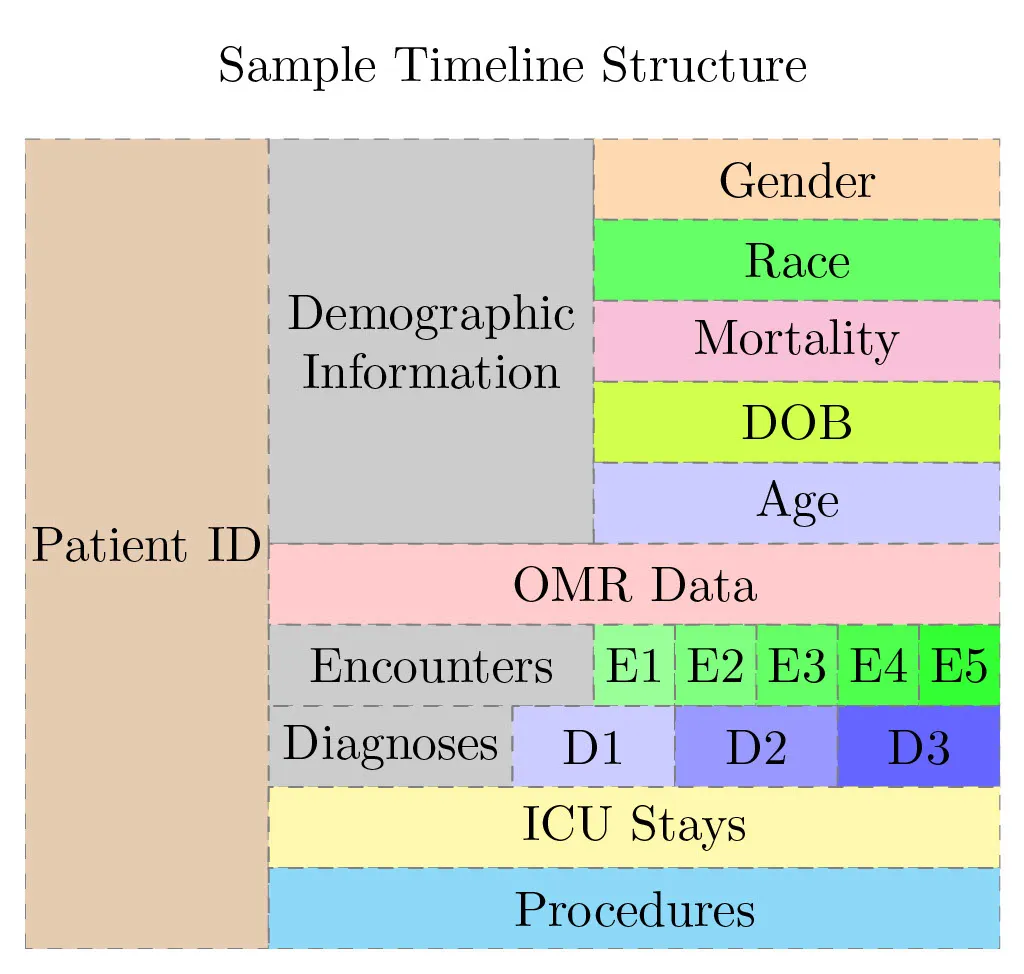
\includegraphics[width=0.4\linewidth]{figures/ehr_timeline.png}
        \caption{Patient EHR Timeline Representation}
        \label{fig:ehr_timeline}
    \end{figure}



      \end{block}

\end{column}




  % \begin{block}{Machine Learning Interpretability}

  %   In machine learning, understanding how models make decisions is crucial. Interpretability reveals the reasoning behind predictions, while explainability provides insights into model behavior.
    

  %   \begin{figure}
  %     \centering
  %     \begin{tikzpicture}[scale=6]
  %       \draw[step=0.25cm,color=gray] (-1,-1) grid (1,1);
  %       \draw (1,0) -- (0.2,0.2) -- (0,1) -- (-0.2,0.2) -- (-1,0)
  %         -- (-0.2,-0.2) -- (0,-1) -- (0.2,-0.2) -- cycle;
  %     \end{tikzpicture}
  %     \caption{A figure caption.}
  %   \end{figure}

  %   Lorem ipsum dolor sit amet, consectetur adipiscing elit. Morbi ultricies
  %   eget libero ac ullamcorper. Integer et euismod ante. Aenean vestibulum
  %   lobortis augue, ut lobortis turpis rhoncus sed. Proin feugiat nibh a
  %   lacinia dignissim. Proin scelerisque, risus eget tempor fermentum, ex
  %   turpis condimentum urna, quis malesuada sapien arcu eu purus.

  % \end{block}

  % \begin{block}{A block containing a list}

  %   Nam vulputate nunc felis, non condimentum lacus porta ultrices. Nullam sed
  %   sagittis metus. Etiam consectetur gravida urna quis suscipit.

  %   \begin{itemize}
  %     \item \textbf{Mauris tempor} risus nulla, sed ornare
  %     \item \textbf{Libero tincidunt} a duis congue vitae
  %     \item \textbf{Dui ac pretium} morbi justo neque, ullamcorper
  %   \end{itemize}

  %   Eget augue porta, bibendum venenatis tortor.

  % \end{block}

  % \begin{alertblock}{A highlighted block}

  %   This block catches your eye, so \textbf{important stuff} should probably go
  %   here.

  %   Curabitur eu libero vehicula, cursus est fringilla, luctus est. Morbi
  %   consectetur mauris quam, at finibus elit auctor ac. Aliquam erat volutpat.
  %   Aenean at nisl ut ex ullamcorper eleifend et eu augue. Aenean quis velit
  %   tristique odio convallis ultrices a ac odio.

  %   \begin{itemize}
  %     \item \textbf{Fusce dapibus tellus} vel tellus semper finibus. In
  %       consequat, nibh sed mattis luctus, augue diam fermentum lectus.
  %     \item \textbf{In euismod erat metus} non ex. Vestibulum luctus augue in
  %       mi condimentum, at sollicitudin lorem viverra.
  %     \item \textbf{Suspendisse vulputate} mauris vel placerat consectetur.
  %       Mauris semper, purus ac hendrerit molestie, elit mi dignissim odio, in
  %       suscipit felis sapien vel ex.
  %   \end{itemize}

  %   Aenean tincidunt risus eros, at gravida lorem sagittis vel. Vestibulum ante
  %   ipsum primis in faucibus orci luctus et ultrices posuere cubilia Curae.

  % \end{alertblock}


\separatorcolumn

\begin{column}{\colwidth}

  \begin{block}{Model Architecture Details}
    
    \textbf{EHR-MoE Design:}
    \begin{itemize}
        \item Built on GPT-2 decoder architecture
        \item Dynamic expert selection via gating network
        \item Sparse expert activation reduces computational load
        \item Maintains model capacity while improving efficiency
    \end{itemize}

        % IMAGE 2: MoE Architecture Diagram
        \begin{figure}
            \centering
            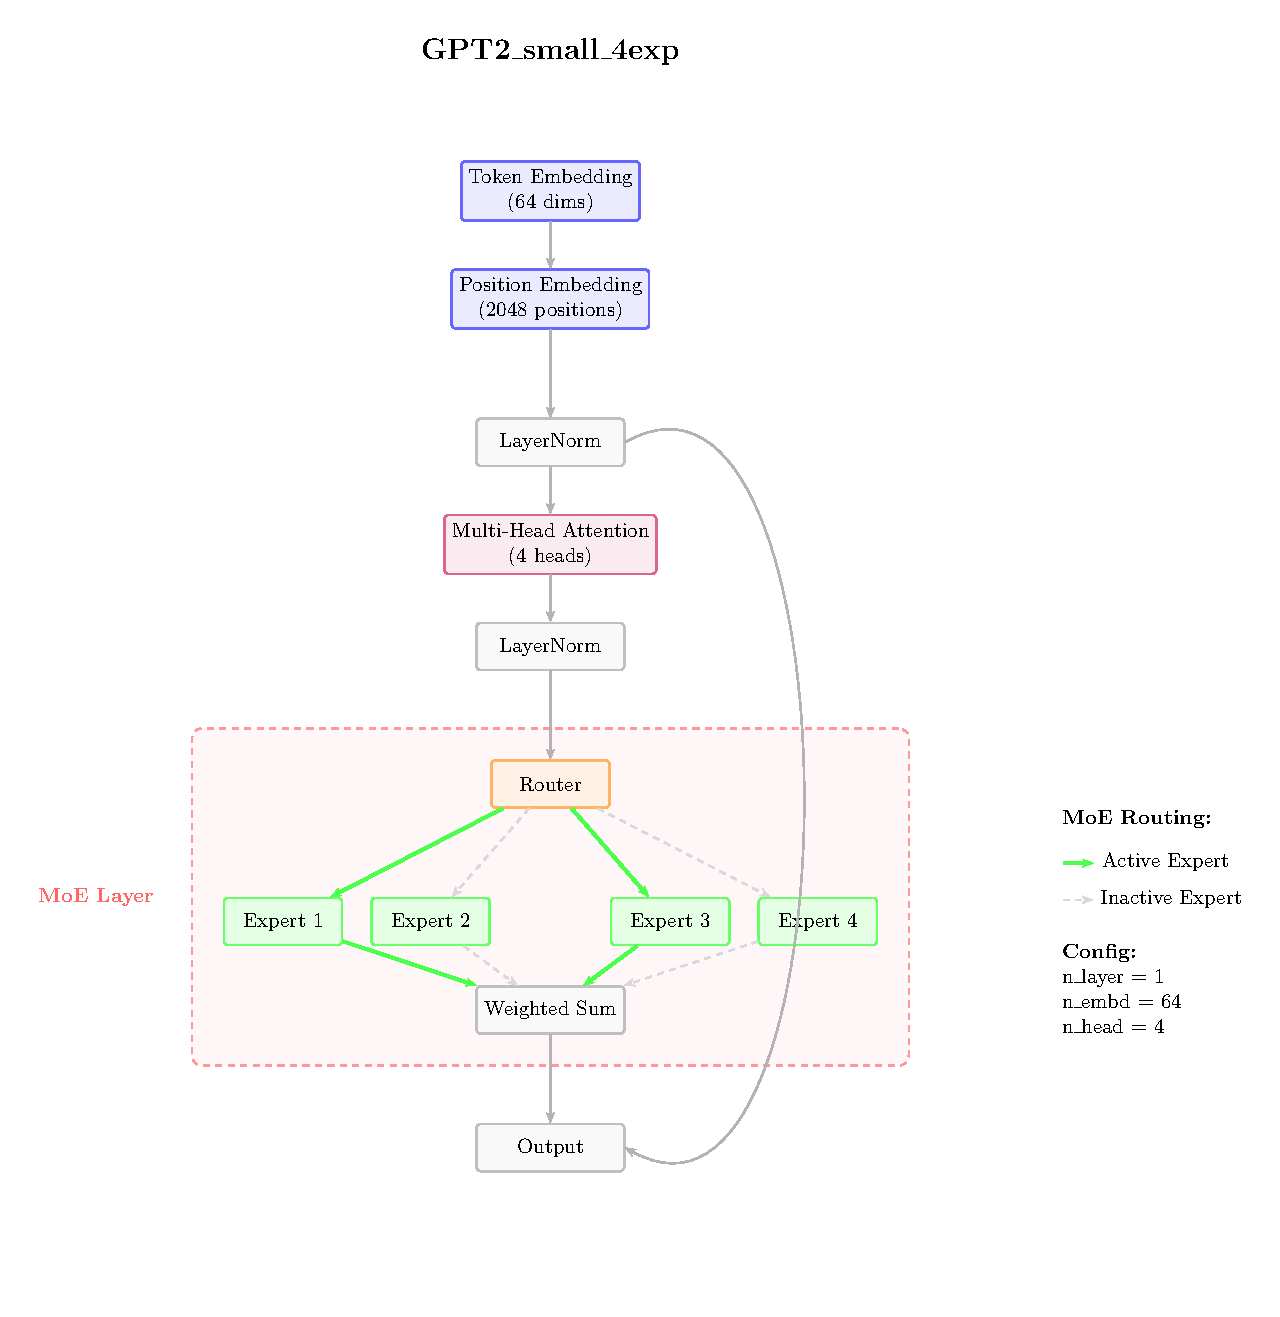
\includegraphics[width=0.6\linewidth]{figures/moe_architecture_tikz.pdf}
            \caption{MoE Architecture for EHR Modeling}
            \label{fig:moe_architecture}
        \end{figure}


       
  \end{block}

  \begin{block}{Data Processing \& Tokenization}
    
    % IMAGE: EHR Data Processing Pipeline
    \begin{figure}
        \centering
        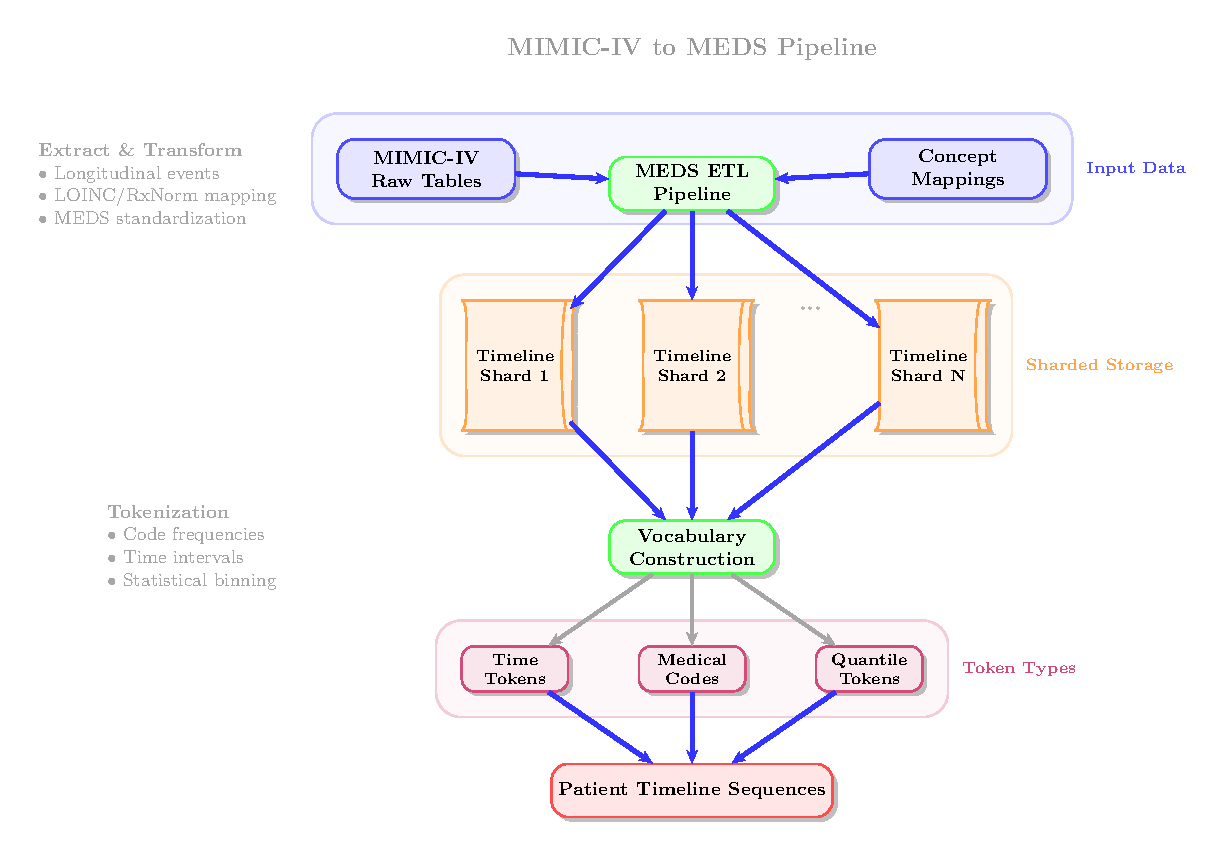
\includegraphics[width=0.75\linewidth]{figures/ehr_preprocessing_pipeline.pdf}
        \caption{EHR Data Processing \& Tokenization Pipeline}
        \label{fig:preprocessing_pipeline}
    \end{figure}

    \textbf{Key Processing Steps:}
    \begin{itemize}
        \item \textbf{Standardization:} ICD-10, CPT, LOINC medical codes
        \item \textbf{Temporal Alignment:} Event timestamps \& admission sequences  
        \item \textbf{Tokenization:} Medical vocabulary with temporal markers
    \end{itemize}

  \end{block}

  \begin{block}{Training Strategy}
    
    \textbf{Pre-training Phase:}
    \begin{itemize}
        \item Next-token prediction on MIMIC-IV sequences
        \item Autoregressive language modeling objective
        \item Expert specialization through gradient-based routing
    \end{itemize}

    \textbf{Fine-tuning Tasks:}
    \begin{itemize}
        \item Hospital mortality prediction
        \item ICU stay duration prediction
        \item Readmission risk assessment
    \end{itemize}

  \end{block}


  % \begin{block}{A block containing an enumerated list}

  %   Vivamus congue volutpat elit non semper. Praesent molestie nec erat ac
  %   interdum. In quis suscipit erat. \textbf{Phasellus mauris felis, molestie
  %   ac pharetra quis}, tempus nec ante. Donec finibus ante vel purus mollis
  %   fermentum. Sed felis mi, pharetra eget nibh a, feugiat eleifend dolor. Nam
  %   mollis condimentum purus quis sodales. Nullam eu felis eu nulla eleifend
  %   bibendum nec eu lorem. Vivamus felis velit, volutpat ut facilisis ac,
  %   commodo in metus.

  %   \begin{enumerate}
  %     \item \textbf{Morbi mauris purus}, egestas at vehicula et, convallis
  %       accumsan orci. Orci varius natoque penatibus et magnis dis parturient
  %       montes, nascetur ridiculus mus.
  %     \item \textbf{Cras vehicula blandit urna ut maximus}. Aliquam blandit nec
  %       massa ac sollicitudin. Curabitur cursus, metus nec imperdiet bibendum,
  %       velit lectus faucibus dolor, quis gravida metus mauris gravida turpis.
  %     \item \textbf{Vestibulum et massa diam}. Phasellus fermentum augue non
  %       nulla accumsan, non rhoncus lectus condimentum.
  %   \end{enumerate}

  % \end{block}

  % \begin{block}{Fusce aliquam magna velit}

  %   Et rutrum ex euismod vel. Pellentesque ultricies, velit in fermentum
  %   vestibulum, lectus nisi pretium nibh, sit amet aliquam lectus augue vel
  %   velit. Suspendisse rhoncus massa porttitor augue feugiat molestie. Sed
  %   molestie ut orci nec malesuada. Sed ultricies feugiat est fringilla
  %   posuere.

  %   \begin{figure}
  %     \centering
  %     \begin{tikzpicture}
  %       \begin{axis}[
  %           scale only axis,
  %           no markers,
  %           domain=0:2*pi,
  %           samples=100,
  %           axis lines=center,
  %           axis line style={-},
  %           ticks=none]
  %         \addplot[red] {sin(deg(x))};
  %         \addplot[blue] {cos(deg(x))};
  %       \end{axis}
  %     \end{tikzpicture}
  %     \caption{Another figure caption.}
  %   \end{figure}

  % \end{block}

  % \begin{block}{Nam cursus consequat egestas}

  %   Nulla eget sem quam. Ut aliquam volutpat nisi vestibulum convallis. Nunc a
  %   lectus et eros facilisis hendrerit eu non urna. Interdum et malesuada fames
  %   ac ante \textit{ipsum primis} in faucibus. Etiam sit amet velit eget sem
  %   euismod tristique. Praesent enim erat, porta vel mattis sed, pharetra sed
  %   ipsum. Morbi commodo condimentum massa, \textit{tempus venenatis} massa
  %   hendrerit quis. Maecenas sed porta est. Praesent mollis interdum lectus,
  %   sit amet sollicitudin risus tincidunt non.

  %   Etiam sit amet tempus lorem, aliquet condimentum velit. Donec et nibh
  %   consequat, sagittis ex eget, dictum orci. Etiam quis semper ante. Ut eu
  %   mauris purus. Proin nec consectetur ligula. Mauris pretium molestie
  %   ullamcorper. Integer nisi neque, aliquet et odio non, sagittis porta justo.

  %   \begin{itemize}
  %     \item \textbf{Sed consequat} id ante vel efficitur. Praesent congue massa
  %       sed est scelerisque, elementum mollis augue iaculis.
  %       \begin{itemize}
  %         \item In sed est finibus, vulputate
  %           nunc gravida, pulvinar lorem. In maximus nunc dolor, sed auctor eros
  %           porttitor quis.
  %         \item Fusce ornare dignissim nisi. Nam sit amet risus vel lacus
  %           tempor tincidunt eu a arcu.
  %         \item Donec rhoncus vestibulum erat, quis aliquam leo
  %           gravida egestas.
  %       \end{itemize}
  %     \item \textbf{Sed luctus, elit sit amet} dictum maximus, diam dolor
  %       faucibus purus, sed lobortis justo erat id turpis.
  %     \item \textbf{Pellentesque facilisis dolor in leo} bibendum congue.
  %       Maecenas congue finibus justo, vitae eleifend urna facilisis at.
  %   \end{itemize}

  % \end{block}

\end{column}

\separatorcolumn

\begin{column}{\colwidth}

  \begin{alertblock}{Key Results}
    
    \textbf{Performance Improvements:}
    \begin{itemize}
        \item Faster convergence during training compared to dense models
        \item Maintained predictive accuracy with reduced computational cost
        \item Superior performance on mortality and ICU stay prediction
    \end{itemize}

    \textbf{Efficiency Gains:}
    \begin{itemize}
        \item Lower GPU memory usage during inference
        \item Reduced computational overhead through sparse activation
        \item Scalable to larger model sizes with constant inference cost
    \end{itemize}
    
  \end{alertblock}

  \begin{block}{Experimental Results}
    
    % IMAGE 3: Performance Comparison Charts
    \begin{figure}
        \centering
        \includegraphics[width=0.6\linewidth]{figures/performance_comparison.png}
        \caption{Performance Comparison: MoE vs Dense Models}
        \label{fig:performance}
    \end{figure}

    \textbf{Evaluation Metrics:}
    \begin{itemize}
        \item AUROC scores for mortality prediction
        \item Training time and convergence speed
        \item Memory utilization during inference
        \item Expert utilization patterns
    \end{itemize}
    
  \end{block}

  \begin{block}{Resource Efficiency}
    
    % IMAGE 4: Resource Usage Charts
    \begin{figure}
        \centering
        \includegraphics[width=0.6\linewidth]{figures/resource_efficiency.png}
        \caption{Computational Resource Usage Analysis}
        \label{fig:resources}
    \end{figure}

    \textbf{Clinical Deployment Benefits:}
    \begin{itemize}
        \item Suitable for resource-constrained clinical settings
        \item Real-time inference capabilities
        \item Reduced infrastructure requirements
        \item Cost-effective scaling for hospital systems
    \end{itemize}
    
  \end{block}

  \begin{block}{Conclusions \& Future Work}
    
    \textbf{Contributions:}
    \begin{itemize}
        \item Novel MoE architecture for EHR foundational models
        \item Demonstrated efficiency gains without accuracy loss
        \item Validated on MIMIC-IV dataset with clinical tasks
    \end{itemize}

    \textbf{Future Directions:}
    \begin{itemize}
        \item Multi-modal integration (clinical notes, imaging)
        \item Federated learning for multi-hospital deployment
        \item Expert interpretability and clinical validation
        \item Real-world clinical trial implementation
    \end{itemize}
    
  \end{block}
        
  % \begin{exampleblock}{A highlighted block containing some math}

  %   A different kind of highlighted block.

  %   $$
  %   \int_{-\infty}^{\infty} e^{-x^2}\,dx = \sqrt{\pi}
  %   $$

  %   Interdum et malesuada fames $\{1, 4, 9, \ldots\}$ ac ante ipsum primis in
  %   faucibus. Cras eleifend dolor eu nulla suscipit suscipit. Sed lobortis non
  %   felis id vulputate.

  %   \heading{A heading inside a block}

  %   Praesent consectetur mi $x^2 + y^2$ metus, nec vestibulum justo viverra
  %   nec. Proin eget nulla pretium, egestas magna aliquam, mollis neque. Vivamus
  %   dictum $\mathbf{u}^\intercal\mathbf{v}$ sagittis odio, vel porta erat
  %   congue sed. Maecenas ut dolor quis arcu auctor porttitor.

  %   \heading{Another heading inside a block}

  %   Sed augue erat, scelerisque a purus ultricies, placerat porttitor neque.
  %   Donec $P(y \mid x)$ fermentum consectetur $\nabla_x P(y \mid x)$ sapien
  %   sagittis egestas. Duis eget leo euismod nunc viverra imperdiet nec id
  %   justo.

  % \end{exampleblock}

  % \begin{block}{Nullam vel erat at velit convallis laoreet}

  %   Class aptent taciti sociosqu ad litora torquent per conubia nostra, per
  %   inceptos himenaeos. Phasellus libero enim, gravida sed erat sit amet,
  %   scelerisque congue diam. Fusce dapibus dui ut augue pulvinar iaculis.

  %   \begin{table}
  %     \centering
  %     \begin{tabular}{l r r c}
  %       \toprule
  %       \textbf{First column} & \textbf{Second column} & \textbf{Third column} & \textbf{Fourth} \\
  %       \midrule
  %       Foo & 13.37 & 384,394 & $\alpha$ \\
  %       Bar & 2.17 & 1,392 & $\beta$ \\
  %       Baz & 3.14 & 83,742 & $\delta$ \\
  %       Qux & 7.59 & 974 & $\gamma$ \\
  %       \bottomrule
  %     \end{tabular}
  %     \caption{A table caption.}
  %   \end{table}

  %   Donec quis posuere ligula. Nunc feugiat elit a mi malesuada consequat. Sed
  %   imperdiet augue ac nibh aliquet tristique. Aenean eu tortor vulputate,
  %   eleifend lorem in, dictum urna. Proin auctor ante in augue tincidunt
  %   tempor. Proin pellentesque vulputate odio, ac gravida nulla posuere
  %   efficitur. Aenean at velit vel dolor blandit molestie. Mauris laoreet
  %   commodo quam, non luctus nibh ullamcorper in. Class aptent taciti sociosqu
  %   ad litora torquent per conubia nostra, per inceptos himenaeos.

  %   Nulla varius finibus volutpat. Mauris molestie lorem tincidunt, iaculis
  %   libero at, gravida ante. Phasellus at felis eu neque suscipit suscipit.
  %   Integer ullamcorper, dui nec pretium ornare, urna dolor consequat libero,
  %   in feugiat elit lorem euismod lacus. Pellentesque sit amet dolor mollis,
  %   auctor urna non, tempus sem.

  % \end{block}

  % \begin{block}{References}

  %   \nocite{*}
  %   \footnotesize{\bibliographystyle{plain}\bibliography{poster}}

  % \end{block}

\end{column}

\separatorcolumn
\end{columns}
\end{frame}

\end{document}


% % Gemini theme
% % https://github.com/anishathalye/gemini
% %
% % We try to keep this Overleaf template in sync with the canonical source on
% % GitHub, but it's recommended that you obtain the template directly from
% % GitHub to ensure that you are using the latest version.

% \documentclass[final]{beamer}

% % ====================
% % Packages
% % ====================

% \usepackage[T1]{fontenc}
% \usepackage{lmodern}
% % \usepackage[size=custom,width=120,height=72,scale=1.0]{beamerposter}
% % \usepackage[size=custom,width=48in,height=36in,scale=1.0]{beamerposter}
% % \usepackage[paperheight=36in,paperwidth=48in,showframe]{geometry}
% \usepackage[size=a0paper, total={36in,48in},]{beamerposter}
% \usepackage{subcaption}
% \usetheme{gemini}
% \usecolortheme{mit}
% \usepackage{graphicx}
% \usepackage{booktabs}
% \usepackage{tikz}
% % \usepackage{pgfplots}
% % \pgfplotsset{width=30cm, compat=1.9}
% \usepackage{fancyhdr}
% \usepackage{standalone}

% \usepackage{pgf}
% \usepackage{lmodern}
% \usepackage{import}
% % \import{figures}{persistence_diagram.pgf}
% % ====================
% % Lengths
% % ====================

% % If you have N columns, choose \sepwidth and \colwidth such that
% % (N+1)*\sepwidth + N*\colwidth = \paperwidth
% \newlength{\sepwidth}
% \newlength{\colwidth}
% \setlength{\sepwidth}{0.025\paperwidth}
% \setlength{\colwidth}{0.3\paperwidth}

% \newcommand{\separatorcolumn}{\begin{column}{\sepwidth}\end{column}}

% % ====================
% % Title
% % ====================
% % \fancyhead[L]{
\includegraphics[width=1.00\pagewidth]{header.png}}

% % \title{Interpreting Deep Learning Models using Persistent homology}

% % \author{Sudhanva M. Athreya \inst{1}  \and Dr. Paul Rosen \inst{1}}

% % \institute[shortinst]{\inst{1} University of Utah }
% % % \samelineand \inst{2} Another Institute}


% % ====================
% % Footer (optional)
% % ====================

% % \footercontent{
% %   \href{https://www.example.com}{https://www.example.com} \hfill
% %   ABC Conference 2025, New York --- XYZ-1234 \hfill
% %   \href{mailto:alyssa.p.hacker@example.com}{alyssa.p.hacker@example.com}}
% % % (can be left out to remove footer)

% % ====================
% % Logo (optional)
% % ====================

% % use this to include logos on the left and/or right side of the header:
% % \logoright{\includegraphics[height=7cm]{logo1.pdf}}
% % \logoleft{\includegraphics[height=7cm]{logo2.pdf}}

% % ====================
% % Body
% % ====================


% % \titlegraphic{
\includegraphics[width=\paperwidth]{header.png}}

% \begin{document}

% \begin{frame}[t]
% \begin{columns}[t]
% \separatorcolumn

% \begin{column}{\colwidth}

%   \begin{alertblock} {Deep Learning Interpretability}
%           In Deep Learning, understanding how models make decisions is crucial. Interpretability reveals the reasoning behind predictions, while explainability provides insights into model behavior. While deep learning models often achieve high accuracy, they can be harder to interpret. Balancing accuracy with interpretability helps ensure responsible and effective AI deployment.
%   \end{alertblock}

  
%     \begin{block} {Persistent Homology}
%         Persistent homology is a method in computational topology that analyzes the shape of data by tracking the creation and disappearance of topological features (like connected components, loops, and voids) across different spatial scales.

%         \begin{figure}
%             \centering
%             
\includegraphics[width=1\linewidth]{figures/ph_process.png}
%             \caption{Filtration}
%             \label{fig:filtration}
%         \end{figure}

%     \end{block}

%     \begin{block} {How Persistent Homology Works}

%     \begin{enumerate}
%         % \item \textbf{Filtration:} Given a set of data points, we create a growing sequence of simplicial complexes. This is done by increasing a proximity threshold, gradually connecting points and forming edges, triangles, and higher-dimensional structures.

%         \item \textbf{Filtration:} Constructing a sequence of simplicial complexes by gradually increasing a proximity threshold, linking points into edges, triangles, and higher-dimensional simplicial complexes. Topological features like \textbf{Connected Components} (0D), \textbf{Loops} (1D), \textbf{Voids} (2D+) are tracked during the filtration process. 


%         % \item \textbf{Topological features tracked during filtration}        
%         % \begin{itemize}
%         %     \item \textbf{Connected Components:} These are isolated groups of points that form as edges are added. 
%         %     \item \textbf{Loops:} These are 1-dimensional holes formed when the filtration process creates a cycle of connections without a boundary.
%         %     \item \textbf{Voids:} Higher-dimensional holes which can appear as simplicial complexes evolve.
%         % \end{itemize}
        
        
%         \item \textbf{Tracking Features:} Topological features \textbf{appear} (birth) and \textbf{disappear} (death) as filtration progresses, and when points are close enough, they form a \textbf{connected component}.
        
%         % As the filtration grows, we track when topological features \textbf{appear} (birth) and \textbf{disappear} (death). When points are close enough, they form a \textbf{connected component}. As the filtration grows, these components may merge into larger connected structures.


%         % \begin{itemize}
%         %     \item \textbf{Persistence Diagram:} : A scatter plot mapping feature lifespans (birth vs. death).
%         %     % \item  \textbf{Persistence Barcodes:} A set of horizontal lines, each representing a topological feature. The left endpoint of each line corresponds to its birth, and the right endpoint to its death. Longer bars represent persistent features, which contribute more to the overall shape of the data, while shorter bars are indicative of less significant, transient features.

%         %     \item  \textbf{Persistence Barcodes:} Horizontal lines representing feature persistence—longer bars indicate more significant structures.
%         % \end{itemize}

%         \item \textbf{Persistence Diagram \& Barcode:} The persistence of topological features is visualized using two main tools: persistence diagrams and barcodes. 
        
%     \end{enumerate}

%     \begin{figure}[h]
%         \begin{center}
%             %% Creator: Matplotlib, PGF backend
%%
%% To include the figure in your LaTeX document, write
%%   \input{<filename>.pgf}
%%
%% Make sure the required packages are loaded in your preamble
%%   \usepackage{pgf}
%%
%% Also ensure that all the required font packages are loaded; for instance,
%% the lmodern package is sometimes necessary when using math font.
%%   \usepackage{lmodern}
%%
%% Figures using additional raster images can only be included by \input if
%% they are in the same directory as the main LaTeX file. For loading figures
%% from other directories you can use the `import` package
%%   \usepackage{import}
%%
%% and then include the figures with
%%   \import{<path to file>}{<filename>.pgf}
%%
%% Matplotlib used the following preamble
%%   \def\mathdefault#1{#1}
%%   \everymath=\expandafter{\the\everymath\displaystyle}
%%   \IfFileExists{scrextend.sty}{
%%     \usepackage[fontsize=11.000000pt]{scrextend}
%%   }{
%%     \renewcommand{\normalsize}{\fontsize{11.000000}{13.200000}\selectfont}
%%     \normalsize
%%   }
%%   
%%   \makeatletter\@ifpackageloaded{underscore}{}{\usepackage[strings]{underscore}}\makeatother
%%
\begingroup%
\makeatletter%
\begin{pgfpicture}%
\pgfpathrectangle{\pgfpointorigin}{\pgfqpoint{12.000000in}{5.000000in}}%
\pgfusepath{use as bounding box, clip}%
\begin{pgfscope}%
\pgfsetbuttcap%
\pgfsetmiterjoin%
\definecolor{currentfill}{rgb}{1.000000,1.000000,1.000000}%
\pgfsetfillcolor{currentfill}%
\pgfsetlinewidth{0.000000pt}%
\definecolor{currentstroke}{rgb}{1.000000,1.000000,1.000000}%
\pgfsetstrokecolor{currentstroke}%
\pgfsetdash{}{0pt}%
\pgfpathmoveto{\pgfqpoint{0.000000in}{0.000000in}}%
\pgfpathlineto{\pgfqpoint{12.000000in}{0.000000in}}%
\pgfpathlineto{\pgfqpoint{12.000000in}{5.000000in}}%
\pgfpathlineto{\pgfqpoint{0.000000in}{5.000000in}}%
\pgfpathlineto{\pgfqpoint{0.000000in}{0.000000in}}%
\pgfpathclose%
\pgfusepath{fill}%
\end{pgfscope}%
\begin{pgfscope}%
\pgfsetbuttcap%
\pgfsetmiterjoin%
\definecolor{currentfill}{rgb}{1.000000,1.000000,1.000000}%
\pgfsetfillcolor{currentfill}%
\pgfsetlinewidth{0.000000pt}%
\definecolor{currentstroke}{rgb}{0.000000,0.000000,0.000000}%
\pgfsetstrokecolor{currentstroke}%
\pgfsetstrokeopacity{0.000000}%
\pgfsetdash{}{0pt}%
\pgfpathmoveto{\pgfqpoint{1.500000in}{0.550000in}}%
\pgfpathlineto{\pgfqpoint{5.727273in}{0.550000in}}%
\pgfpathlineto{\pgfqpoint{5.727273in}{4.400000in}}%
\pgfpathlineto{\pgfqpoint{1.500000in}{4.400000in}}%
\pgfpathlineto{\pgfqpoint{1.500000in}{0.550000in}}%
\pgfpathclose%
\pgfusepath{fill}%
\end{pgfscope}%
\begin{pgfscope}%
\pgfpathrectangle{\pgfqpoint{1.500000in}{0.550000in}}{\pgfqpoint{4.227273in}{3.850000in}}%
\pgfusepath{clip}%
\pgfsetbuttcap%
\pgfsetmiterjoin%
\definecolor{currentfill}{rgb}{0.827451,0.827451,0.827451}%
\pgfsetfillcolor{currentfill}%
\pgfsetlinewidth{1.003750pt}%
\definecolor{currentstroke}{rgb}{0.827451,0.827451,0.827451}%
\pgfsetstrokecolor{currentstroke}%
\pgfsetdash{}{0pt}%
\pgfpathmoveto{\pgfqpoint{1.500000in}{0.550000in}}%
\pgfpathlineto{\pgfqpoint{5.727273in}{0.550000in}}%
\pgfpathlineto{\pgfqpoint{5.727273in}{4.092000in}}%
\pgfpathlineto{\pgfqpoint{1.500000in}{0.550000in}}%
\pgfpathclose%
\pgfusepath{stroke,fill}%
\end{pgfscope}%
\begin{pgfscope}%
\pgfpathrectangle{\pgfqpoint{1.500000in}{0.550000in}}{\pgfqpoint{4.227273in}{3.850000in}}%
\pgfusepath{clip}%
\pgfsetbuttcap%
\pgfsetroundjoin%
\definecolor{currentfill}{rgb}{0.215686,0.494118,0.721569}%
\pgfsetfillcolor{currentfill}%
\pgfsetfillopacity{0.600000}%
\pgfsetlinewidth{1.003750pt}%
\definecolor{currentstroke}{rgb}{0.215686,0.494118,0.721569}%
\pgfsetstrokecolor{currentstroke}%
\pgfsetstrokeopacity{0.600000}%
\pgfsetdash{}{0pt}%
\pgfpathmoveto{\pgfqpoint{5.504444in}{4.204333in}}%
\pgfpathcurveto{\pgfqpoint{5.515494in}{4.204333in}}{\pgfqpoint{5.526093in}{4.208724in}}{\pgfqpoint{5.533907in}{4.216537in}}%
\pgfpathcurveto{\pgfqpoint{5.541721in}{4.224351in}}{\pgfqpoint{5.546111in}{4.234950in}}{\pgfqpoint{5.546111in}{4.246000in}}%
\pgfpathcurveto{\pgfqpoint{5.546111in}{4.257050in}}{\pgfqpoint{5.541721in}{4.267649in}}{\pgfqpoint{5.533907in}{4.275463in}}%
\pgfpathcurveto{\pgfqpoint{5.526093in}{4.283276in}}{\pgfqpoint{5.515494in}{4.287667in}}{\pgfqpoint{5.504444in}{4.287667in}}%
\pgfpathcurveto{\pgfqpoint{5.493394in}{4.287667in}}{\pgfqpoint{5.482795in}{4.283276in}}{\pgfqpoint{5.474981in}{4.275463in}}%
\pgfpathcurveto{\pgfqpoint{5.467168in}{4.267649in}}{\pgfqpoint{5.462777in}{4.257050in}}{\pgfqpoint{5.462777in}{4.246000in}}%
\pgfpathcurveto{\pgfqpoint{5.462777in}{4.234950in}}{\pgfqpoint{5.467168in}{4.224351in}}{\pgfqpoint{5.474981in}{4.216537in}}%
\pgfpathcurveto{\pgfqpoint{5.482795in}{4.208724in}}{\pgfqpoint{5.493394in}{4.204333in}}{\pgfqpoint{5.504444in}{4.204333in}}%
\pgfpathlineto{\pgfqpoint{5.504444in}{4.204333in}}%
\pgfpathclose%
\pgfusepath{stroke,fill}%
\end{pgfscope}%
\begin{pgfscope}%
\pgfpathrectangle{\pgfqpoint{1.500000in}{0.550000in}}{\pgfqpoint{4.227273in}{3.850000in}}%
\pgfusepath{clip}%
\pgfsetbuttcap%
\pgfsetroundjoin%
\definecolor{currentfill}{rgb}{0.215686,0.494118,0.721569}%
\pgfsetfillcolor{currentfill}%
\pgfsetfillopacity{0.600000}%
\pgfsetlinewidth{1.003750pt}%
\definecolor{currentstroke}{rgb}{0.215686,0.494118,0.721569}%
\pgfsetstrokecolor{currentstroke}%
\pgfsetstrokeopacity{0.600000}%
\pgfsetdash{}{0pt}%
\pgfpathmoveto{\pgfqpoint{4.630463in}{4.204333in}}%
\pgfpathcurveto{\pgfqpoint{4.641513in}{4.204333in}}{\pgfqpoint{4.652112in}{4.208724in}}{\pgfqpoint{4.659926in}{4.216537in}}%
\pgfpathcurveto{\pgfqpoint{4.667739in}{4.224351in}}{\pgfqpoint{4.672130in}{4.234950in}}{\pgfqpoint{4.672130in}{4.246000in}}%
\pgfpathcurveto{\pgfqpoint{4.672130in}{4.257050in}}{\pgfqpoint{4.667739in}{4.267649in}}{\pgfqpoint{4.659926in}{4.275463in}}%
\pgfpathcurveto{\pgfqpoint{4.652112in}{4.283276in}}{\pgfqpoint{4.641513in}{4.287667in}}{\pgfqpoint{4.630463in}{4.287667in}}%
\pgfpathcurveto{\pgfqpoint{4.619413in}{4.287667in}}{\pgfqpoint{4.608814in}{4.283276in}}{\pgfqpoint{4.601000in}{4.275463in}}%
\pgfpathcurveto{\pgfqpoint{4.593187in}{4.267649in}}{\pgfqpoint{4.588796in}{4.257050in}}{\pgfqpoint{4.588796in}{4.246000in}}%
\pgfpathcurveto{\pgfqpoint{4.588796in}{4.234950in}}{\pgfqpoint{4.593187in}{4.224351in}}{\pgfqpoint{4.601000in}{4.216537in}}%
\pgfpathcurveto{\pgfqpoint{4.608814in}{4.208724in}}{\pgfqpoint{4.619413in}{4.204333in}}{\pgfqpoint{4.630463in}{4.204333in}}%
\pgfpathlineto{\pgfqpoint{4.630463in}{4.204333in}}%
\pgfpathclose%
\pgfusepath{stroke,fill}%
\end{pgfscope}%
\begin{pgfscope}%
\pgfpathrectangle{\pgfqpoint{1.500000in}{0.550000in}}{\pgfqpoint{4.227273in}{3.850000in}}%
\pgfusepath{clip}%
\pgfsetbuttcap%
\pgfsetroundjoin%
\definecolor{currentfill}{rgb}{0.215686,0.494118,0.721569}%
\pgfsetfillcolor{currentfill}%
\pgfsetfillopacity{0.600000}%
\pgfsetlinewidth{1.003750pt}%
\definecolor{currentstroke}{rgb}{0.215686,0.494118,0.721569}%
\pgfsetstrokecolor{currentstroke}%
\pgfsetstrokeopacity{0.600000}%
\pgfsetdash{}{0pt}%
\pgfpathmoveto{\pgfqpoint{4.851384in}{4.204333in}}%
\pgfpathcurveto{\pgfqpoint{4.862434in}{4.204333in}}{\pgfqpoint{4.873033in}{4.208724in}}{\pgfqpoint{4.880846in}{4.216537in}}%
\pgfpathcurveto{\pgfqpoint{4.888660in}{4.224351in}}{\pgfqpoint{4.893050in}{4.234950in}}{\pgfqpoint{4.893050in}{4.246000in}}%
\pgfpathcurveto{\pgfqpoint{4.893050in}{4.257050in}}{\pgfqpoint{4.888660in}{4.267649in}}{\pgfqpoint{4.880846in}{4.275463in}}%
\pgfpathcurveto{\pgfqpoint{4.873033in}{4.283276in}}{\pgfqpoint{4.862434in}{4.287667in}}{\pgfqpoint{4.851384in}{4.287667in}}%
\pgfpathcurveto{\pgfqpoint{4.840334in}{4.287667in}}{\pgfqpoint{4.829735in}{4.283276in}}{\pgfqpoint{4.821921in}{4.275463in}}%
\pgfpathcurveto{\pgfqpoint{4.814107in}{4.267649in}}{\pgfqpoint{4.809717in}{4.257050in}}{\pgfqpoint{4.809717in}{4.246000in}}%
\pgfpathcurveto{\pgfqpoint{4.809717in}{4.234950in}}{\pgfqpoint{4.814107in}{4.224351in}}{\pgfqpoint{4.821921in}{4.216537in}}%
\pgfpathcurveto{\pgfqpoint{4.829735in}{4.208724in}}{\pgfqpoint{4.840334in}{4.204333in}}{\pgfqpoint{4.851384in}{4.204333in}}%
\pgfpathlineto{\pgfqpoint{4.851384in}{4.204333in}}%
\pgfpathclose%
\pgfusepath{stroke,fill}%
\end{pgfscope}%
\begin{pgfscope}%
\pgfpathrectangle{\pgfqpoint{1.500000in}{0.550000in}}{\pgfqpoint{4.227273in}{3.850000in}}%
\pgfusepath{clip}%
\pgfsetbuttcap%
\pgfsetroundjoin%
\definecolor{currentfill}{rgb}{0.215686,0.494118,0.721569}%
\pgfsetfillcolor{currentfill}%
\pgfsetfillopacity{0.600000}%
\pgfsetlinewidth{1.003750pt}%
\definecolor{currentstroke}{rgb}{0.215686,0.494118,0.721569}%
\pgfsetstrokecolor{currentstroke}%
\pgfsetstrokeopacity{0.600000}%
\pgfsetdash{}{0pt}%
\pgfpathmoveto{\pgfqpoint{4.882783in}{4.204333in}}%
\pgfpathcurveto{\pgfqpoint{4.893833in}{4.204333in}}{\pgfqpoint{4.904433in}{4.208724in}}{\pgfqpoint{4.912246in}{4.216537in}}%
\pgfpathcurveto{\pgfqpoint{4.920060in}{4.224351in}}{\pgfqpoint{4.924450in}{4.234950in}}{\pgfqpoint{4.924450in}{4.246000in}}%
\pgfpathcurveto{\pgfqpoint{4.924450in}{4.257050in}}{\pgfqpoint{4.920060in}{4.267649in}}{\pgfqpoint{4.912246in}{4.275463in}}%
\pgfpathcurveto{\pgfqpoint{4.904433in}{4.283276in}}{\pgfqpoint{4.893833in}{4.287667in}}{\pgfqpoint{4.882783in}{4.287667in}}%
\pgfpathcurveto{\pgfqpoint{4.871733in}{4.287667in}}{\pgfqpoint{4.861134in}{4.283276in}}{\pgfqpoint{4.853321in}{4.275463in}}%
\pgfpathcurveto{\pgfqpoint{4.845507in}{4.267649in}}{\pgfqpoint{4.841117in}{4.257050in}}{\pgfqpoint{4.841117in}{4.246000in}}%
\pgfpathcurveto{\pgfqpoint{4.841117in}{4.234950in}}{\pgfqpoint{4.845507in}{4.224351in}}{\pgfqpoint{4.853321in}{4.216537in}}%
\pgfpathcurveto{\pgfqpoint{4.861134in}{4.208724in}}{\pgfqpoint{4.871733in}{4.204333in}}{\pgfqpoint{4.882783in}{4.204333in}}%
\pgfpathlineto{\pgfqpoint{4.882783in}{4.204333in}}%
\pgfpathclose%
\pgfusepath{stroke,fill}%
\end{pgfscope}%
\begin{pgfscope}%
\pgfpathrectangle{\pgfqpoint{1.500000in}{0.550000in}}{\pgfqpoint{4.227273in}{3.850000in}}%
\pgfusepath{clip}%
\pgfsetbuttcap%
\pgfsetroundjoin%
\definecolor{currentfill}{rgb}{0.215686,0.494118,0.721569}%
\pgfsetfillcolor{currentfill}%
\pgfsetfillopacity{0.600000}%
\pgfsetlinewidth{1.003750pt}%
\definecolor{currentstroke}{rgb}{0.215686,0.494118,0.721569}%
\pgfsetstrokecolor{currentstroke}%
\pgfsetstrokeopacity{0.600000}%
\pgfsetdash{}{0pt}%
\pgfpathmoveto{\pgfqpoint{5.049484in}{4.204333in}}%
\pgfpathcurveto{\pgfqpoint{5.060534in}{4.204333in}}{\pgfqpoint{5.071133in}{4.208724in}}{\pgfqpoint{5.078947in}{4.216537in}}%
\pgfpathcurveto{\pgfqpoint{5.086761in}{4.224351in}}{\pgfqpoint{5.091151in}{4.234950in}}{\pgfqpoint{5.091151in}{4.246000in}}%
\pgfpathcurveto{\pgfqpoint{5.091151in}{4.257050in}}{\pgfqpoint{5.086761in}{4.267649in}}{\pgfqpoint{5.078947in}{4.275463in}}%
\pgfpathcurveto{\pgfqpoint{5.071133in}{4.283276in}}{\pgfqpoint{5.060534in}{4.287667in}}{\pgfqpoint{5.049484in}{4.287667in}}%
\pgfpathcurveto{\pgfqpoint{5.038434in}{4.287667in}}{\pgfqpoint{5.027835in}{4.283276in}}{\pgfqpoint{5.020022in}{4.275463in}}%
\pgfpathcurveto{\pgfqpoint{5.012208in}{4.267649in}}{\pgfqpoint{5.007818in}{4.257050in}}{\pgfqpoint{5.007818in}{4.246000in}}%
\pgfpathcurveto{\pgfqpoint{5.007818in}{4.234950in}}{\pgfqpoint{5.012208in}{4.224351in}}{\pgfqpoint{5.020022in}{4.216537in}}%
\pgfpathcurveto{\pgfqpoint{5.027835in}{4.208724in}}{\pgfqpoint{5.038434in}{4.204333in}}{\pgfqpoint{5.049484in}{4.204333in}}%
\pgfpathlineto{\pgfqpoint{5.049484in}{4.204333in}}%
\pgfpathclose%
\pgfusepath{stroke,fill}%
\end{pgfscope}%
\begin{pgfscope}%
\pgfpathrectangle{\pgfqpoint{1.500000in}{0.550000in}}{\pgfqpoint{4.227273in}{3.850000in}}%
\pgfusepath{clip}%
\pgfsetbuttcap%
\pgfsetroundjoin%
\definecolor{currentfill}{rgb}{0.215686,0.494118,0.721569}%
\pgfsetfillcolor{currentfill}%
\pgfsetfillopacity{0.600000}%
\pgfsetlinewidth{1.003750pt}%
\definecolor{currentstroke}{rgb}{0.215686,0.494118,0.721569}%
\pgfsetstrokecolor{currentstroke}%
\pgfsetstrokeopacity{0.600000}%
\pgfsetdash{}{0pt}%
\pgfpathmoveto{\pgfqpoint{5.100682in}{4.204333in}}%
\pgfpathcurveto{\pgfqpoint{5.111732in}{4.204333in}}{\pgfqpoint{5.122331in}{4.208724in}}{\pgfqpoint{5.130145in}{4.216537in}}%
\pgfpathcurveto{\pgfqpoint{5.137958in}{4.224351in}}{\pgfqpoint{5.142349in}{4.234950in}}{\pgfqpoint{5.142349in}{4.246000in}}%
\pgfpathcurveto{\pgfqpoint{5.142349in}{4.257050in}}{\pgfqpoint{5.137958in}{4.267649in}}{\pgfqpoint{5.130145in}{4.275463in}}%
\pgfpathcurveto{\pgfqpoint{5.122331in}{4.283276in}}{\pgfqpoint{5.111732in}{4.287667in}}{\pgfqpoint{5.100682in}{4.287667in}}%
\pgfpathcurveto{\pgfqpoint{5.089632in}{4.287667in}}{\pgfqpoint{5.079033in}{4.283276in}}{\pgfqpoint{5.071219in}{4.275463in}}%
\pgfpathcurveto{\pgfqpoint{5.063406in}{4.267649in}}{\pgfqpoint{5.059015in}{4.257050in}}{\pgfqpoint{5.059015in}{4.246000in}}%
\pgfpathcurveto{\pgfqpoint{5.059015in}{4.234950in}}{\pgfqpoint{5.063406in}{4.224351in}}{\pgfqpoint{5.071219in}{4.216537in}}%
\pgfpathcurveto{\pgfqpoint{5.079033in}{4.208724in}}{\pgfqpoint{5.089632in}{4.204333in}}{\pgfqpoint{5.100682in}{4.204333in}}%
\pgfpathlineto{\pgfqpoint{5.100682in}{4.204333in}}%
\pgfpathclose%
\pgfusepath{stroke,fill}%
\end{pgfscope}%
\begin{pgfscope}%
\pgfpathrectangle{\pgfqpoint{1.500000in}{0.550000in}}{\pgfqpoint{4.227273in}{3.850000in}}%
\pgfusepath{clip}%
\pgfsetbuttcap%
\pgfsetroundjoin%
\definecolor{currentfill}{rgb}{0.215686,0.494118,0.721569}%
\pgfsetfillcolor{currentfill}%
\pgfsetfillopacity{0.600000}%
\pgfsetlinewidth{1.003750pt}%
\definecolor{currentstroke}{rgb}{0.215686,0.494118,0.721569}%
\pgfsetstrokecolor{currentstroke}%
\pgfsetstrokeopacity{0.600000}%
\pgfsetdash{}{0pt}%
\pgfpathmoveto{\pgfqpoint{5.119956in}{4.204333in}}%
\pgfpathcurveto{\pgfqpoint{5.131006in}{4.204333in}}{\pgfqpoint{5.141605in}{4.208724in}}{\pgfqpoint{5.149419in}{4.216537in}}%
\pgfpathcurveto{\pgfqpoint{5.157232in}{4.224351in}}{\pgfqpoint{5.161623in}{4.234950in}}{\pgfqpoint{5.161623in}{4.246000in}}%
\pgfpathcurveto{\pgfqpoint{5.161623in}{4.257050in}}{\pgfqpoint{5.157232in}{4.267649in}}{\pgfqpoint{5.149419in}{4.275463in}}%
\pgfpathcurveto{\pgfqpoint{5.141605in}{4.283276in}}{\pgfqpoint{5.131006in}{4.287667in}}{\pgfqpoint{5.119956in}{4.287667in}}%
\pgfpathcurveto{\pgfqpoint{5.108906in}{4.287667in}}{\pgfqpoint{5.098307in}{4.283276in}}{\pgfqpoint{5.090493in}{4.275463in}}%
\pgfpathcurveto{\pgfqpoint{5.082680in}{4.267649in}}{\pgfqpoint{5.078289in}{4.257050in}}{\pgfqpoint{5.078289in}{4.246000in}}%
\pgfpathcurveto{\pgfqpoint{5.078289in}{4.234950in}}{\pgfqpoint{5.082680in}{4.224351in}}{\pgfqpoint{5.090493in}{4.216537in}}%
\pgfpathcurveto{\pgfqpoint{5.098307in}{4.208724in}}{\pgfqpoint{5.108906in}{4.204333in}}{\pgfqpoint{5.119956in}{4.204333in}}%
\pgfpathlineto{\pgfqpoint{5.119956in}{4.204333in}}%
\pgfpathclose%
\pgfusepath{stroke,fill}%
\end{pgfscope}%
\begin{pgfscope}%
\pgfpathrectangle{\pgfqpoint{1.500000in}{0.550000in}}{\pgfqpoint{4.227273in}{3.850000in}}%
\pgfusepath{clip}%
\pgfsetbuttcap%
\pgfsetroundjoin%
\definecolor{currentfill}{rgb}{0.215686,0.494118,0.721569}%
\pgfsetfillcolor{currentfill}%
\pgfsetfillopacity{0.600000}%
\pgfsetlinewidth{1.003750pt}%
\definecolor{currentstroke}{rgb}{0.215686,0.494118,0.721569}%
\pgfsetstrokecolor{currentstroke}%
\pgfsetstrokeopacity{0.600000}%
\pgfsetdash{}{0pt}%
\pgfpathmoveto{\pgfqpoint{5.175790in}{4.204333in}}%
\pgfpathcurveto{\pgfqpoint{5.186840in}{4.204333in}}{\pgfqpoint{5.197439in}{4.208724in}}{\pgfqpoint{5.205253in}{4.216537in}}%
\pgfpathcurveto{\pgfqpoint{5.213066in}{4.224351in}}{\pgfqpoint{5.217457in}{4.234950in}}{\pgfqpoint{5.217457in}{4.246000in}}%
\pgfpathcurveto{\pgfqpoint{5.217457in}{4.257050in}}{\pgfqpoint{5.213066in}{4.267649in}}{\pgfqpoint{5.205253in}{4.275463in}}%
\pgfpathcurveto{\pgfqpoint{5.197439in}{4.283276in}}{\pgfqpoint{5.186840in}{4.287667in}}{\pgfqpoint{5.175790in}{4.287667in}}%
\pgfpathcurveto{\pgfqpoint{5.164740in}{4.287667in}}{\pgfqpoint{5.154141in}{4.283276in}}{\pgfqpoint{5.146327in}{4.275463in}}%
\pgfpathcurveto{\pgfqpoint{5.138514in}{4.267649in}}{\pgfqpoint{5.134123in}{4.257050in}}{\pgfqpoint{5.134123in}{4.246000in}}%
\pgfpathcurveto{\pgfqpoint{5.134123in}{4.234950in}}{\pgfqpoint{5.138514in}{4.224351in}}{\pgfqpoint{5.146327in}{4.216537in}}%
\pgfpathcurveto{\pgfqpoint{5.154141in}{4.208724in}}{\pgfqpoint{5.164740in}{4.204333in}}{\pgfqpoint{5.175790in}{4.204333in}}%
\pgfpathlineto{\pgfqpoint{5.175790in}{4.204333in}}%
\pgfpathclose%
\pgfusepath{stroke,fill}%
\end{pgfscope}%
\begin{pgfscope}%
\pgfpathrectangle{\pgfqpoint{1.500000in}{0.550000in}}{\pgfqpoint{4.227273in}{3.850000in}}%
\pgfusepath{clip}%
\pgfsetbuttcap%
\pgfsetroundjoin%
\definecolor{currentfill}{rgb}{0.215686,0.494118,0.721569}%
\pgfsetfillcolor{currentfill}%
\pgfsetfillopacity{0.600000}%
\pgfsetlinewidth{1.003750pt}%
\definecolor{currentstroke}{rgb}{0.215686,0.494118,0.721569}%
\pgfsetstrokecolor{currentstroke}%
\pgfsetstrokeopacity{0.600000}%
\pgfsetdash{}{0pt}%
\pgfpathmoveto{\pgfqpoint{5.254095in}{4.204333in}}%
\pgfpathcurveto{\pgfqpoint{5.265146in}{4.204333in}}{\pgfqpoint{5.275745in}{4.208724in}}{\pgfqpoint{5.283558in}{4.216537in}}%
\pgfpathcurveto{\pgfqpoint{5.291372in}{4.224351in}}{\pgfqpoint{5.295762in}{4.234950in}}{\pgfqpoint{5.295762in}{4.246000in}}%
\pgfpathcurveto{\pgfqpoint{5.295762in}{4.257050in}}{\pgfqpoint{5.291372in}{4.267649in}}{\pgfqpoint{5.283558in}{4.275463in}}%
\pgfpathcurveto{\pgfqpoint{5.275745in}{4.283276in}}{\pgfqpoint{5.265146in}{4.287667in}}{\pgfqpoint{5.254095in}{4.287667in}}%
\pgfpathcurveto{\pgfqpoint{5.243045in}{4.287667in}}{\pgfqpoint{5.232446in}{4.283276in}}{\pgfqpoint{5.224633in}{4.275463in}}%
\pgfpathcurveto{\pgfqpoint{5.216819in}{4.267649in}}{\pgfqpoint{5.212429in}{4.257050in}}{\pgfqpoint{5.212429in}{4.246000in}}%
\pgfpathcurveto{\pgfqpoint{5.212429in}{4.234950in}}{\pgfqpoint{5.216819in}{4.224351in}}{\pgfqpoint{5.224633in}{4.216537in}}%
\pgfpathcurveto{\pgfqpoint{5.232446in}{4.208724in}}{\pgfqpoint{5.243045in}{4.204333in}}{\pgfqpoint{5.254095in}{4.204333in}}%
\pgfpathlineto{\pgfqpoint{5.254095in}{4.204333in}}%
\pgfpathclose%
\pgfusepath{stroke,fill}%
\end{pgfscope}%
\begin{pgfscope}%
\pgfpathrectangle{\pgfqpoint{1.500000in}{0.550000in}}{\pgfqpoint{4.227273in}{3.850000in}}%
\pgfusepath{clip}%
\pgfsetbuttcap%
\pgfsetroundjoin%
\definecolor{currentfill}{rgb}{0.215686,0.494118,0.721569}%
\pgfsetfillcolor{currentfill}%
\pgfsetfillopacity{0.600000}%
\pgfsetlinewidth{1.003750pt}%
\definecolor{currentstroke}{rgb}{0.215686,0.494118,0.721569}%
\pgfsetstrokecolor{currentstroke}%
\pgfsetstrokeopacity{0.600000}%
\pgfsetdash{}{0pt}%
\pgfpathmoveto{\pgfqpoint{5.285116in}{4.204333in}}%
\pgfpathcurveto{\pgfqpoint{5.296167in}{4.204333in}}{\pgfqpoint{5.306766in}{4.208724in}}{\pgfqpoint{5.314579in}{4.216537in}}%
\pgfpathcurveto{\pgfqpoint{5.322393in}{4.224351in}}{\pgfqpoint{5.326783in}{4.234950in}}{\pgfqpoint{5.326783in}{4.246000in}}%
\pgfpathcurveto{\pgfqpoint{5.326783in}{4.257050in}}{\pgfqpoint{5.322393in}{4.267649in}}{\pgfqpoint{5.314579in}{4.275463in}}%
\pgfpathcurveto{\pgfqpoint{5.306766in}{4.283276in}}{\pgfqpoint{5.296167in}{4.287667in}}{\pgfqpoint{5.285116in}{4.287667in}}%
\pgfpathcurveto{\pgfqpoint{5.274066in}{4.287667in}}{\pgfqpoint{5.263467in}{4.283276in}}{\pgfqpoint{5.255654in}{4.275463in}}%
\pgfpathcurveto{\pgfqpoint{5.247840in}{4.267649in}}{\pgfqpoint{5.243450in}{4.257050in}}{\pgfqpoint{5.243450in}{4.246000in}}%
\pgfpathcurveto{\pgfqpoint{5.243450in}{4.234950in}}{\pgfqpoint{5.247840in}{4.224351in}}{\pgfqpoint{5.255654in}{4.216537in}}%
\pgfpathcurveto{\pgfqpoint{5.263467in}{4.208724in}}{\pgfqpoint{5.274066in}{4.204333in}}{\pgfqpoint{5.285116in}{4.204333in}}%
\pgfpathlineto{\pgfqpoint{5.285116in}{4.204333in}}%
\pgfpathclose%
\pgfusepath{stroke,fill}%
\end{pgfscope}%
\begin{pgfscope}%
\pgfpathrectangle{\pgfqpoint{1.500000in}{0.550000in}}{\pgfqpoint{4.227273in}{3.850000in}}%
\pgfusepath{clip}%
\pgfsetbuttcap%
\pgfsetroundjoin%
\definecolor{currentfill}{rgb}{0.215686,0.494118,0.721569}%
\pgfsetfillcolor{currentfill}%
\pgfsetfillopacity{0.600000}%
\pgfsetlinewidth{1.003750pt}%
\definecolor{currentstroke}{rgb}{0.215686,0.494118,0.721569}%
\pgfsetstrokecolor{currentstroke}%
\pgfsetstrokeopacity{0.600000}%
\pgfsetdash{}{0pt}%
\pgfpathmoveto{\pgfqpoint{5.290815in}{4.204333in}}%
\pgfpathcurveto{\pgfqpoint{5.301865in}{4.204333in}}{\pgfqpoint{5.312464in}{4.208724in}}{\pgfqpoint{5.320278in}{4.216537in}}%
\pgfpathcurveto{\pgfqpoint{5.328091in}{4.224351in}}{\pgfqpoint{5.332482in}{4.234950in}}{\pgfqpoint{5.332482in}{4.246000in}}%
\pgfpathcurveto{\pgfqpoint{5.332482in}{4.257050in}}{\pgfqpoint{5.328091in}{4.267649in}}{\pgfqpoint{5.320278in}{4.275463in}}%
\pgfpathcurveto{\pgfqpoint{5.312464in}{4.283276in}}{\pgfqpoint{5.301865in}{4.287667in}}{\pgfqpoint{5.290815in}{4.287667in}}%
\pgfpathcurveto{\pgfqpoint{5.279765in}{4.287667in}}{\pgfqpoint{5.269166in}{4.283276in}}{\pgfqpoint{5.261352in}{4.275463in}}%
\pgfpathcurveto{\pgfqpoint{5.253538in}{4.267649in}}{\pgfqpoint{5.249148in}{4.257050in}}{\pgfqpoint{5.249148in}{4.246000in}}%
\pgfpathcurveto{\pgfqpoint{5.249148in}{4.234950in}}{\pgfqpoint{5.253538in}{4.224351in}}{\pgfqpoint{5.261352in}{4.216537in}}%
\pgfpathcurveto{\pgfqpoint{5.269166in}{4.208724in}}{\pgfqpoint{5.279765in}{4.204333in}}{\pgfqpoint{5.290815in}{4.204333in}}%
\pgfpathlineto{\pgfqpoint{5.290815in}{4.204333in}}%
\pgfpathclose%
\pgfusepath{stroke,fill}%
\end{pgfscope}%
\begin{pgfscope}%
\pgfpathrectangle{\pgfqpoint{1.500000in}{0.550000in}}{\pgfqpoint{4.227273in}{3.850000in}}%
\pgfusepath{clip}%
\pgfsetbuttcap%
\pgfsetroundjoin%
\definecolor{currentfill}{rgb}{0.215686,0.494118,0.721569}%
\pgfsetfillcolor{currentfill}%
\pgfsetfillopacity{0.600000}%
\pgfsetlinewidth{1.003750pt}%
\definecolor{currentstroke}{rgb}{0.215686,0.494118,0.721569}%
\pgfsetstrokecolor{currentstroke}%
\pgfsetstrokeopacity{0.600000}%
\pgfsetdash{}{0pt}%
\pgfpathmoveto{\pgfqpoint{5.292627in}{4.204333in}}%
\pgfpathcurveto{\pgfqpoint{5.303677in}{4.204333in}}{\pgfqpoint{5.314276in}{4.208724in}}{\pgfqpoint{5.322090in}{4.216537in}}%
\pgfpathcurveto{\pgfqpoint{5.329904in}{4.224351in}}{\pgfqpoint{5.334294in}{4.234950in}}{\pgfqpoint{5.334294in}{4.246000in}}%
\pgfpathcurveto{\pgfqpoint{5.334294in}{4.257050in}}{\pgfqpoint{5.329904in}{4.267649in}}{\pgfqpoint{5.322090in}{4.275463in}}%
\pgfpathcurveto{\pgfqpoint{5.314276in}{4.283276in}}{\pgfqpoint{5.303677in}{4.287667in}}{\pgfqpoint{5.292627in}{4.287667in}}%
\pgfpathcurveto{\pgfqpoint{5.281577in}{4.287667in}}{\pgfqpoint{5.270978in}{4.283276in}}{\pgfqpoint{5.263165in}{4.275463in}}%
\pgfpathcurveto{\pgfqpoint{5.255351in}{4.267649in}}{\pgfqpoint{5.250961in}{4.257050in}}{\pgfqpoint{5.250961in}{4.246000in}}%
\pgfpathcurveto{\pgfqpoint{5.250961in}{4.234950in}}{\pgfqpoint{5.255351in}{4.224351in}}{\pgfqpoint{5.263165in}{4.216537in}}%
\pgfpathcurveto{\pgfqpoint{5.270978in}{4.208724in}}{\pgfqpoint{5.281577in}{4.204333in}}{\pgfqpoint{5.292627in}{4.204333in}}%
\pgfpathlineto{\pgfqpoint{5.292627in}{4.204333in}}%
\pgfpathclose%
\pgfusepath{stroke,fill}%
\end{pgfscope}%
\begin{pgfscope}%
\pgfpathrectangle{\pgfqpoint{1.500000in}{0.550000in}}{\pgfqpoint{4.227273in}{3.850000in}}%
\pgfusepath{clip}%
\pgfsetbuttcap%
\pgfsetroundjoin%
\definecolor{currentfill}{rgb}{0.215686,0.494118,0.721569}%
\pgfsetfillcolor{currentfill}%
\pgfsetfillopacity{0.600000}%
\pgfsetlinewidth{1.003750pt}%
\definecolor{currentstroke}{rgb}{0.215686,0.494118,0.721569}%
\pgfsetstrokecolor{currentstroke}%
\pgfsetstrokeopacity{0.600000}%
\pgfsetdash{}{0pt}%
\pgfpathmoveto{\pgfqpoint{5.308611in}{4.204333in}}%
\pgfpathcurveto{\pgfqpoint{5.319661in}{4.204333in}}{\pgfqpoint{5.330260in}{4.208724in}}{\pgfqpoint{5.338074in}{4.216537in}}%
\pgfpathcurveto{\pgfqpoint{5.345887in}{4.224351in}}{\pgfqpoint{5.350277in}{4.234950in}}{\pgfqpoint{5.350277in}{4.246000in}}%
\pgfpathcurveto{\pgfqpoint{5.350277in}{4.257050in}}{\pgfqpoint{5.345887in}{4.267649in}}{\pgfqpoint{5.338074in}{4.275463in}}%
\pgfpathcurveto{\pgfqpoint{5.330260in}{4.283276in}}{\pgfqpoint{5.319661in}{4.287667in}}{\pgfqpoint{5.308611in}{4.287667in}}%
\pgfpathcurveto{\pgfqpoint{5.297561in}{4.287667in}}{\pgfqpoint{5.286962in}{4.283276in}}{\pgfqpoint{5.279148in}{4.275463in}}%
\pgfpathcurveto{\pgfqpoint{5.271334in}{4.267649in}}{\pgfqpoint{5.266944in}{4.257050in}}{\pgfqpoint{5.266944in}{4.246000in}}%
\pgfpathcurveto{\pgfqpoint{5.266944in}{4.234950in}}{\pgfqpoint{5.271334in}{4.224351in}}{\pgfqpoint{5.279148in}{4.216537in}}%
\pgfpathcurveto{\pgfqpoint{5.286962in}{4.208724in}}{\pgfqpoint{5.297561in}{4.204333in}}{\pgfqpoint{5.308611in}{4.204333in}}%
\pgfpathlineto{\pgfqpoint{5.308611in}{4.204333in}}%
\pgfpathclose%
\pgfusepath{stroke,fill}%
\end{pgfscope}%
\begin{pgfscope}%
\pgfpathrectangle{\pgfqpoint{1.500000in}{0.550000in}}{\pgfqpoint{4.227273in}{3.850000in}}%
\pgfusepath{clip}%
\pgfsetbuttcap%
\pgfsetroundjoin%
\definecolor{currentfill}{rgb}{0.215686,0.494118,0.721569}%
\pgfsetfillcolor{currentfill}%
\pgfsetfillopacity{0.600000}%
\pgfsetlinewidth{1.003750pt}%
\definecolor{currentstroke}{rgb}{0.215686,0.494118,0.721569}%
\pgfsetstrokecolor{currentstroke}%
\pgfsetstrokeopacity{0.600000}%
\pgfsetdash{}{0pt}%
\pgfpathmoveto{\pgfqpoint{5.453173in}{4.204333in}}%
\pgfpathcurveto{\pgfqpoint{5.464223in}{4.204333in}}{\pgfqpoint{5.474822in}{4.208724in}}{\pgfqpoint{5.482635in}{4.216537in}}%
\pgfpathcurveto{\pgfqpoint{5.490449in}{4.224351in}}{\pgfqpoint{5.494839in}{4.234950in}}{\pgfqpoint{5.494839in}{4.246000in}}%
\pgfpathcurveto{\pgfqpoint{5.494839in}{4.257050in}}{\pgfqpoint{5.490449in}{4.267649in}}{\pgfqpoint{5.482635in}{4.275463in}}%
\pgfpathcurveto{\pgfqpoint{5.474822in}{4.283276in}}{\pgfqpoint{5.464223in}{4.287667in}}{\pgfqpoint{5.453173in}{4.287667in}}%
\pgfpathcurveto{\pgfqpoint{5.442122in}{4.287667in}}{\pgfqpoint{5.431523in}{4.283276in}}{\pgfqpoint{5.423710in}{4.275463in}}%
\pgfpathcurveto{\pgfqpoint{5.415896in}{4.267649in}}{\pgfqpoint{5.411506in}{4.257050in}}{\pgfqpoint{5.411506in}{4.246000in}}%
\pgfpathcurveto{\pgfqpoint{5.411506in}{4.234950in}}{\pgfqpoint{5.415896in}{4.224351in}}{\pgfqpoint{5.423710in}{4.216537in}}%
\pgfpathcurveto{\pgfqpoint{5.431523in}{4.208724in}}{\pgfqpoint{5.442122in}{4.204333in}}{\pgfqpoint{5.453173in}{4.204333in}}%
\pgfpathlineto{\pgfqpoint{5.453173in}{4.204333in}}%
\pgfpathclose%
\pgfusepath{stroke,fill}%
\end{pgfscope}%
\begin{pgfscope}%
\pgfpathrectangle{\pgfqpoint{1.500000in}{0.550000in}}{\pgfqpoint{4.227273in}{3.850000in}}%
\pgfusepath{clip}%
\pgfsetbuttcap%
\pgfsetroundjoin%
\definecolor{currentfill}{rgb}{0.215686,0.494118,0.721569}%
\pgfsetfillcolor{currentfill}%
\pgfsetfillopacity{0.600000}%
\pgfsetlinewidth{1.003750pt}%
\definecolor{currentstroke}{rgb}{0.215686,0.494118,0.721569}%
\pgfsetstrokecolor{currentstroke}%
\pgfsetstrokeopacity{0.600000}%
\pgfsetdash{}{0pt}%
\pgfpathmoveto{\pgfqpoint{5.495618in}{4.204333in}}%
\pgfpathcurveto{\pgfqpoint{5.506668in}{4.204333in}}{\pgfqpoint{5.517268in}{4.208724in}}{\pgfqpoint{5.525081in}{4.216537in}}%
\pgfpathcurveto{\pgfqpoint{5.532895in}{4.224351in}}{\pgfqpoint{5.537285in}{4.234950in}}{\pgfqpoint{5.537285in}{4.246000in}}%
\pgfpathcurveto{\pgfqpoint{5.537285in}{4.257050in}}{\pgfqpoint{5.532895in}{4.267649in}}{\pgfqpoint{5.525081in}{4.275463in}}%
\pgfpathcurveto{\pgfqpoint{5.517268in}{4.283276in}}{\pgfqpoint{5.506668in}{4.287667in}}{\pgfqpoint{5.495618in}{4.287667in}}%
\pgfpathcurveto{\pgfqpoint{5.484568in}{4.287667in}}{\pgfqpoint{5.473969in}{4.283276in}}{\pgfqpoint{5.466156in}{4.275463in}}%
\pgfpathcurveto{\pgfqpoint{5.458342in}{4.267649in}}{\pgfqpoint{5.453952in}{4.257050in}}{\pgfqpoint{5.453952in}{4.246000in}}%
\pgfpathcurveto{\pgfqpoint{5.453952in}{4.234950in}}{\pgfqpoint{5.458342in}{4.224351in}}{\pgfqpoint{5.466156in}{4.216537in}}%
\pgfpathcurveto{\pgfqpoint{5.473969in}{4.208724in}}{\pgfqpoint{5.484568in}{4.204333in}}{\pgfqpoint{5.495618in}{4.204333in}}%
\pgfpathlineto{\pgfqpoint{5.495618in}{4.204333in}}%
\pgfpathclose%
\pgfusepath{stroke,fill}%
\end{pgfscope}%
\begin{pgfscope}%
\pgfpathrectangle{\pgfqpoint{1.500000in}{0.550000in}}{\pgfqpoint{4.227273in}{3.850000in}}%
\pgfusepath{clip}%
\pgfsetbuttcap%
\pgfsetroundjoin%
\definecolor{currentfill}{rgb}{0.215686,0.494118,0.721569}%
\pgfsetfillcolor{currentfill}%
\pgfsetfillopacity{0.600000}%
\pgfsetlinewidth{1.003750pt}%
\definecolor{currentstroke}{rgb}{0.215686,0.494118,0.721569}%
\pgfsetstrokecolor{currentstroke}%
\pgfsetstrokeopacity{0.600000}%
\pgfsetdash{}{0pt}%
\pgfpathmoveto{\pgfqpoint{5.273451in}{4.204333in}}%
\pgfpathcurveto{\pgfqpoint{5.284502in}{4.204333in}}{\pgfqpoint{5.295101in}{4.208724in}}{\pgfqpoint{5.302914in}{4.216537in}}%
\pgfpathcurveto{\pgfqpoint{5.310728in}{4.224351in}}{\pgfqpoint{5.315118in}{4.234950in}}{\pgfqpoint{5.315118in}{4.246000in}}%
\pgfpathcurveto{\pgfqpoint{5.315118in}{4.257050in}}{\pgfqpoint{5.310728in}{4.267649in}}{\pgfqpoint{5.302914in}{4.275463in}}%
\pgfpathcurveto{\pgfqpoint{5.295101in}{4.283276in}}{\pgfqpoint{5.284502in}{4.287667in}}{\pgfqpoint{5.273451in}{4.287667in}}%
\pgfpathcurveto{\pgfqpoint{5.262401in}{4.287667in}}{\pgfqpoint{5.251802in}{4.283276in}}{\pgfqpoint{5.243989in}{4.275463in}}%
\pgfpathcurveto{\pgfqpoint{5.236175in}{4.267649in}}{\pgfqpoint{5.231785in}{4.257050in}}{\pgfqpoint{5.231785in}{4.246000in}}%
\pgfpathcurveto{\pgfqpoint{5.231785in}{4.234950in}}{\pgfqpoint{5.236175in}{4.224351in}}{\pgfqpoint{5.243989in}{4.216537in}}%
\pgfpathcurveto{\pgfqpoint{5.251802in}{4.208724in}}{\pgfqpoint{5.262401in}{4.204333in}}{\pgfqpoint{5.273451in}{4.204333in}}%
\pgfpathlineto{\pgfqpoint{5.273451in}{4.204333in}}%
\pgfpathclose%
\pgfusepath{stroke,fill}%
\end{pgfscope}%
\begin{pgfscope}%
\pgfpathrectangle{\pgfqpoint{1.500000in}{0.550000in}}{\pgfqpoint{4.227273in}{3.850000in}}%
\pgfusepath{clip}%
\pgfsetbuttcap%
\pgfsetroundjoin%
\definecolor{currentfill}{rgb}{0.894118,0.101961,0.109804}%
\pgfsetfillcolor{currentfill}%
\pgfsetfillopacity{0.600000}%
\pgfsetlinewidth{1.003750pt}%
\definecolor{currentstroke}{rgb}{0.894118,0.101961,0.109804}%
\pgfsetstrokecolor{currentstroke}%
\pgfsetstrokeopacity{0.600000}%
\pgfsetdash{}{0pt}%
\pgfpathmoveto{\pgfqpoint{1.867589in}{4.204333in}}%
\pgfpathcurveto{\pgfqpoint{1.878639in}{4.204333in}}{\pgfqpoint{1.889238in}{4.208724in}}{\pgfqpoint{1.897052in}{4.216537in}}%
\pgfpathcurveto{\pgfqpoint{1.904865in}{4.224351in}}{\pgfqpoint{1.909256in}{4.234950in}}{\pgfqpoint{1.909256in}{4.246000in}}%
\pgfpathcurveto{\pgfqpoint{1.909256in}{4.257050in}}{\pgfqpoint{1.904865in}{4.267649in}}{\pgfqpoint{1.897052in}{4.275463in}}%
\pgfpathcurveto{\pgfqpoint{1.889238in}{4.283276in}}{\pgfqpoint{1.878639in}{4.287667in}}{\pgfqpoint{1.867589in}{4.287667in}}%
\pgfpathcurveto{\pgfqpoint{1.856539in}{4.287667in}}{\pgfqpoint{1.845940in}{4.283276in}}{\pgfqpoint{1.838126in}{4.275463in}}%
\pgfpathcurveto{\pgfqpoint{1.830313in}{4.267649in}}{\pgfqpoint{1.825922in}{4.257050in}}{\pgfqpoint{1.825922in}{4.246000in}}%
\pgfpathcurveto{\pgfqpoint{1.825922in}{4.234950in}}{\pgfqpoint{1.830313in}{4.224351in}}{\pgfqpoint{1.838126in}{4.216537in}}%
\pgfpathcurveto{\pgfqpoint{1.845940in}{4.208724in}}{\pgfqpoint{1.856539in}{4.204333in}}{\pgfqpoint{1.867589in}{4.204333in}}%
\pgfpathlineto{\pgfqpoint{1.867589in}{4.204333in}}%
\pgfpathclose%
\pgfusepath{stroke,fill}%
\end{pgfscope}%
\begin{pgfscope}%
\pgfpathrectangle{\pgfqpoint{1.500000in}{0.550000in}}{\pgfqpoint{4.227273in}{3.850000in}}%
\pgfusepath{clip}%
\pgfsetbuttcap%
\pgfsetroundjoin%
\definecolor{currentfill}{rgb}{0.894118,0.101961,0.109804}%
\pgfsetfillcolor{currentfill}%
\pgfsetfillopacity{0.600000}%
\pgfsetlinewidth{1.003750pt}%
\definecolor{currentstroke}{rgb}{0.894118,0.101961,0.109804}%
\pgfsetstrokecolor{currentstroke}%
\pgfsetstrokeopacity{0.600000}%
\pgfsetdash{}{0pt}%
\pgfpathmoveto{\pgfqpoint{1.867589in}{4.204333in}}%
\pgfpathcurveto{\pgfqpoint{1.878639in}{4.204333in}}{\pgfqpoint{1.889238in}{4.208724in}}{\pgfqpoint{1.897052in}{4.216537in}}%
\pgfpathcurveto{\pgfqpoint{1.904865in}{4.224351in}}{\pgfqpoint{1.909256in}{4.234950in}}{\pgfqpoint{1.909256in}{4.246000in}}%
\pgfpathcurveto{\pgfqpoint{1.909256in}{4.257050in}}{\pgfqpoint{1.904865in}{4.267649in}}{\pgfqpoint{1.897052in}{4.275463in}}%
\pgfpathcurveto{\pgfqpoint{1.889238in}{4.283276in}}{\pgfqpoint{1.878639in}{4.287667in}}{\pgfqpoint{1.867589in}{4.287667in}}%
\pgfpathcurveto{\pgfqpoint{1.856539in}{4.287667in}}{\pgfqpoint{1.845940in}{4.283276in}}{\pgfqpoint{1.838126in}{4.275463in}}%
\pgfpathcurveto{\pgfqpoint{1.830313in}{4.267649in}}{\pgfqpoint{1.825922in}{4.257050in}}{\pgfqpoint{1.825922in}{4.246000in}}%
\pgfpathcurveto{\pgfqpoint{1.825922in}{4.234950in}}{\pgfqpoint{1.830313in}{4.224351in}}{\pgfqpoint{1.838126in}{4.216537in}}%
\pgfpathcurveto{\pgfqpoint{1.845940in}{4.208724in}}{\pgfqpoint{1.856539in}{4.204333in}}{\pgfqpoint{1.867589in}{4.204333in}}%
\pgfpathlineto{\pgfqpoint{1.867589in}{4.204333in}}%
\pgfpathclose%
\pgfusepath{stroke,fill}%
\end{pgfscope}%
\begin{pgfscope}%
\pgfpathrectangle{\pgfqpoint{1.500000in}{0.550000in}}{\pgfqpoint{4.227273in}{3.850000in}}%
\pgfusepath{clip}%
\pgfsetbuttcap%
\pgfsetroundjoin%
\definecolor{currentfill}{rgb}{0.894118,0.101961,0.109804}%
\pgfsetfillcolor{currentfill}%
\pgfsetfillopacity{0.600000}%
\pgfsetlinewidth{1.003750pt}%
\definecolor{currentstroke}{rgb}{0.894118,0.101961,0.109804}%
\pgfsetstrokecolor{currentstroke}%
\pgfsetstrokeopacity{0.600000}%
\pgfsetdash{}{0pt}%
\pgfpathmoveto{\pgfqpoint{1.867589in}{4.204333in}}%
\pgfpathcurveto{\pgfqpoint{1.878639in}{4.204333in}}{\pgfqpoint{1.889238in}{4.208724in}}{\pgfqpoint{1.897052in}{4.216537in}}%
\pgfpathcurveto{\pgfqpoint{1.904865in}{4.224351in}}{\pgfqpoint{1.909256in}{4.234950in}}{\pgfqpoint{1.909256in}{4.246000in}}%
\pgfpathcurveto{\pgfqpoint{1.909256in}{4.257050in}}{\pgfqpoint{1.904865in}{4.267649in}}{\pgfqpoint{1.897052in}{4.275463in}}%
\pgfpathcurveto{\pgfqpoint{1.889238in}{4.283276in}}{\pgfqpoint{1.878639in}{4.287667in}}{\pgfqpoint{1.867589in}{4.287667in}}%
\pgfpathcurveto{\pgfqpoint{1.856539in}{4.287667in}}{\pgfqpoint{1.845940in}{4.283276in}}{\pgfqpoint{1.838126in}{4.275463in}}%
\pgfpathcurveto{\pgfqpoint{1.830313in}{4.267649in}}{\pgfqpoint{1.825922in}{4.257050in}}{\pgfqpoint{1.825922in}{4.246000in}}%
\pgfpathcurveto{\pgfqpoint{1.825922in}{4.234950in}}{\pgfqpoint{1.830313in}{4.224351in}}{\pgfqpoint{1.838126in}{4.216537in}}%
\pgfpathcurveto{\pgfqpoint{1.845940in}{4.208724in}}{\pgfqpoint{1.856539in}{4.204333in}}{\pgfqpoint{1.867589in}{4.204333in}}%
\pgfpathlineto{\pgfqpoint{1.867589in}{4.204333in}}%
\pgfpathclose%
\pgfusepath{stroke,fill}%
\end{pgfscope}%
\begin{pgfscope}%
\pgfpathrectangle{\pgfqpoint{1.500000in}{0.550000in}}{\pgfqpoint{4.227273in}{3.850000in}}%
\pgfusepath{clip}%
\pgfsetbuttcap%
\pgfsetroundjoin%
\definecolor{currentfill}{rgb}{0.894118,0.101961,0.109804}%
\pgfsetfillcolor{currentfill}%
\pgfsetfillopacity{0.600000}%
\pgfsetlinewidth{1.003750pt}%
\definecolor{currentstroke}{rgb}{0.894118,0.101961,0.109804}%
\pgfsetstrokecolor{currentstroke}%
\pgfsetstrokeopacity{0.600000}%
\pgfsetdash{}{0pt}%
\pgfpathmoveto{\pgfqpoint{1.867589in}{3.896333in}}%
\pgfpathcurveto{\pgfqpoint{1.878639in}{3.896333in}}{\pgfqpoint{1.889238in}{3.900724in}}{\pgfqpoint{1.897052in}{3.908537in}}%
\pgfpathcurveto{\pgfqpoint{1.904865in}{3.916351in}}{\pgfqpoint{1.909256in}{3.926950in}}{\pgfqpoint{1.909256in}{3.938000in}}%
\pgfpathcurveto{\pgfqpoint{1.909256in}{3.949050in}}{\pgfqpoint{1.904865in}{3.959649in}}{\pgfqpoint{1.897052in}{3.967463in}}%
\pgfpathcurveto{\pgfqpoint{1.889238in}{3.975276in}}{\pgfqpoint{1.878639in}{3.979667in}}{\pgfqpoint{1.867589in}{3.979667in}}%
\pgfpathcurveto{\pgfqpoint{1.856539in}{3.979667in}}{\pgfqpoint{1.845940in}{3.975276in}}{\pgfqpoint{1.838126in}{3.967463in}}%
\pgfpathcurveto{\pgfqpoint{1.830313in}{3.959649in}}{\pgfqpoint{1.825922in}{3.949050in}}{\pgfqpoint{1.825922in}{3.938000in}}%
\pgfpathcurveto{\pgfqpoint{1.825922in}{3.926950in}}{\pgfqpoint{1.830313in}{3.916351in}}{\pgfqpoint{1.838126in}{3.908537in}}%
\pgfpathcurveto{\pgfqpoint{1.845940in}{3.900724in}}{\pgfqpoint{1.856539in}{3.896333in}}{\pgfqpoint{1.867589in}{3.896333in}}%
\pgfpathlineto{\pgfqpoint{1.867589in}{3.896333in}}%
\pgfpathclose%
\pgfusepath{stroke,fill}%
\end{pgfscope}%
\begin{pgfscope}%
\pgfpathrectangle{\pgfqpoint{1.500000in}{0.550000in}}{\pgfqpoint{4.227273in}{3.850000in}}%
\pgfusepath{clip}%
\pgfsetbuttcap%
\pgfsetroundjoin%
\definecolor{currentfill}{rgb}{0.894118,0.101961,0.109804}%
\pgfsetfillcolor{currentfill}%
\pgfsetfillopacity{0.600000}%
\pgfsetlinewidth{1.003750pt}%
\definecolor{currentstroke}{rgb}{0.894118,0.101961,0.109804}%
\pgfsetstrokecolor{currentstroke}%
\pgfsetstrokeopacity{0.600000}%
\pgfsetdash{}{0pt}%
\pgfpathmoveto{\pgfqpoint{1.867589in}{3.839936in}}%
\pgfpathcurveto{\pgfqpoint{1.878639in}{3.839936in}}{\pgfqpoint{1.889238in}{3.844327in}}{\pgfqpoint{1.897052in}{3.852140in}}%
\pgfpathcurveto{\pgfqpoint{1.904865in}{3.859954in}}{\pgfqpoint{1.909256in}{3.870553in}}{\pgfqpoint{1.909256in}{3.881603in}}%
\pgfpathcurveto{\pgfqpoint{1.909256in}{3.892653in}}{\pgfqpoint{1.904865in}{3.903252in}}{\pgfqpoint{1.897052in}{3.911066in}}%
\pgfpathcurveto{\pgfqpoint{1.889238in}{3.918879in}}{\pgfqpoint{1.878639in}{3.923270in}}{\pgfqpoint{1.867589in}{3.923270in}}%
\pgfpathcurveto{\pgfqpoint{1.856539in}{3.923270in}}{\pgfqpoint{1.845940in}{3.918879in}}{\pgfqpoint{1.838126in}{3.911066in}}%
\pgfpathcurveto{\pgfqpoint{1.830313in}{3.903252in}}{\pgfqpoint{1.825922in}{3.892653in}}{\pgfqpoint{1.825922in}{3.881603in}}%
\pgfpathcurveto{\pgfqpoint{1.825922in}{3.870553in}}{\pgfqpoint{1.830313in}{3.859954in}}{\pgfqpoint{1.838126in}{3.852140in}}%
\pgfpathcurveto{\pgfqpoint{1.845940in}{3.844327in}}{\pgfqpoint{1.856539in}{3.839936in}}{\pgfqpoint{1.867589in}{3.839936in}}%
\pgfpathlineto{\pgfqpoint{1.867589in}{3.839936in}}%
\pgfpathclose%
\pgfusepath{stroke,fill}%
\end{pgfscope}%
\begin{pgfscope}%
\pgfpathrectangle{\pgfqpoint{1.500000in}{0.550000in}}{\pgfqpoint{4.227273in}{3.850000in}}%
\pgfusepath{clip}%
\pgfsetbuttcap%
\pgfsetroundjoin%
\definecolor{currentfill}{rgb}{0.894118,0.101961,0.109804}%
\pgfsetfillcolor{currentfill}%
\pgfsetfillopacity{0.600000}%
\pgfsetlinewidth{1.003750pt}%
\definecolor{currentstroke}{rgb}{0.894118,0.101961,0.109804}%
\pgfsetstrokecolor{currentstroke}%
\pgfsetstrokeopacity{0.600000}%
\pgfsetdash{}{0pt}%
\pgfpathmoveto{\pgfqpoint{1.867589in}{3.750780in}}%
\pgfpathcurveto{\pgfqpoint{1.878639in}{3.750780in}}{\pgfqpoint{1.889238in}{3.755170in}}{\pgfqpoint{1.897052in}{3.762984in}}%
\pgfpathcurveto{\pgfqpoint{1.904865in}{3.770798in}}{\pgfqpoint{1.909256in}{3.781397in}}{\pgfqpoint{1.909256in}{3.792447in}}%
\pgfpathcurveto{\pgfqpoint{1.909256in}{3.803497in}}{\pgfqpoint{1.904865in}{3.814096in}}{\pgfqpoint{1.897052in}{3.821910in}}%
\pgfpathcurveto{\pgfqpoint{1.889238in}{3.829723in}}{\pgfqpoint{1.878639in}{3.834113in}}{\pgfqpoint{1.867589in}{3.834113in}}%
\pgfpathcurveto{\pgfqpoint{1.856539in}{3.834113in}}{\pgfqpoint{1.845940in}{3.829723in}}{\pgfqpoint{1.838126in}{3.821910in}}%
\pgfpathcurveto{\pgfqpoint{1.830313in}{3.814096in}}{\pgfqpoint{1.825922in}{3.803497in}}{\pgfqpoint{1.825922in}{3.792447in}}%
\pgfpathcurveto{\pgfqpoint{1.825922in}{3.781397in}}{\pgfqpoint{1.830313in}{3.770798in}}{\pgfqpoint{1.838126in}{3.762984in}}%
\pgfpathcurveto{\pgfqpoint{1.845940in}{3.755170in}}{\pgfqpoint{1.856539in}{3.750780in}}{\pgfqpoint{1.867589in}{3.750780in}}%
\pgfpathlineto{\pgfqpoint{1.867589in}{3.750780in}}%
\pgfpathclose%
\pgfusepath{stroke,fill}%
\end{pgfscope}%
\begin{pgfscope}%
\pgfpathrectangle{\pgfqpoint{1.500000in}{0.550000in}}{\pgfqpoint{4.227273in}{3.850000in}}%
\pgfusepath{clip}%
\pgfsetbuttcap%
\pgfsetroundjoin%
\definecolor{currentfill}{rgb}{0.894118,0.101961,0.109804}%
\pgfsetfillcolor{currentfill}%
\pgfsetfillopacity{0.600000}%
\pgfsetlinewidth{1.003750pt}%
\definecolor{currentstroke}{rgb}{0.894118,0.101961,0.109804}%
\pgfsetstrokecolor{currentstroke}%
\pgfsetstrokeopacity{0.600000}%
\pgfsetdash{}{0pt}%
\pgfpathmoveto{\pgfqpoint{1.867589in}{3.673784in}}%
\pgfpathcurveto{\pgfqpoint{1.878639in}{3.673784in}}{\pgfqpoint{1.889238in}{3.678174in}}{\pgfqpoint{1.897052in}{3.685988in}}%
\pgfpathcurveto{\pgfqpoint{1.904865in}{3.693801in}}{\pgfqpoint{1.909256in}{3.704401in}}{\pgfqpoint{1.909256in}{3.715451in}}%
\pgfpathcurveto{\pgfqpoint{1.909256in}{3.726501in}}{\pgfqpoint{1.904865in}{3.737100in}}{\pgfqpoint{1.897052in}{3.744913in}}%
\pgfpathcurveto{\pgfqpoint{1.889238in}{3.752727in}}{\pgfqpoint{1.878639in}{3.757117in}}{\pgfqpoint{1.867589in}{3.757117in}}%
\pgfpathcurveto{\pgfqpoint{1.856539in}{3.757117in}}{\pgfqpoint{1.845940in}{3.752727in}}{\pgfqpoint{1.838126in}{3.744913in}}%
\pgfpathcurveto{\pgfqpoint{1.830313in}{3.737100in}}{\pgfqpoint{1.825922in}{3.726501in}}{\pgfqpoint{1.825922in}{3.715451in}}%
\pgfpathcurveto{\pgfqpoint{1.825922in}{3.704401in}}{\pgfqpoint{1.830313in}{3.693801in}}{\pgfqpoint{1.838126in}{3.685988in}}%
\pgfpathcurveto{\pgfqpoint{1.845940in}{3.678174in}}{\pgfqpoint{1.856539in}{3.673784in}}{\pgfqpoint{1.867589in}{3.673784in}}%
\pgfpathlineto{\pgfqpoint{1.867589in}{3.673784in}}%
\pgfpathclose%
\pgfusepath{stroke,fill}%
\end{pgfscope}%
\begin{pgfscope}%
\pgfpathrectangle{\pgfqpoint{1.500000in}{0.550000in}}{\pgfqpoint{4.227273in}{3.850000in}}%
\pgfusepath{clip}%
\pgfsetbuttcap%
\pgfsetroundjoin%
\definecolor{currentfill}{rgb}{0.894118,0.101961,0.109804}%
\pgfsetfillcolor{currentfill}%
\pgfsetfillopacity{0.600000}%
\pgfsetlinewidth{1.003750pt}%
\definecolor{currentstroke}{rgb}{0.894118,0.101961,0.109804}%
\pgfsetstrokecolor{currentstroke}%
\pgfsetstrokeopacity{0.600000}%
\pgfsetdash{}{0pt}%
\pgfpathmoveto{\pgfqpoint{1.867589in}{3.670550in}}%
\pgfpathcurveto{\pgfqpoint{1.878639in}{3.670550in}}{\pgfqpoint{1.889238in}{3.674940in}}{\pgfqpoint{1.897052in}{3.682754in}}%
\pgfpathcurveto{\pgfqpoint{1.904865in}{3.690567in}}{\pgfqpoint{1.909256in}{3.701166in}}{\pgfqpoint{1.909256in}{3.712216in}}%
\pgfpathcurveto{\pgfqpoint{1.909256in}{3.723267in}}{\pgfqpoint{1.904865in}{3.733866in}}{\pgfqpoint{1.897052in}{3.741679in}}%
\pgfpathcurveto{\pgfqpoint{1.889238in}{3.749493in}}{\pgfqpoint{1.878639in}{3.753883in}}{\pgfqpoint{1.867589in}{3.753883in}}%
\pgfpathcurveto{\pgfqpoint{1.856539in}{3.753883in}}{\pgfqpoint{1.845940in}{3.749493in}}{\pgfqpoint{1.838126in}{3.741679in}}%
\pgfpathcurveto{\pgfqpoint{1.830313in}{3.733866in}}{\pgfqpoint{1.825922in}{3.723267in}}{\pgfqpoint{1.825922in}{3.712216in}}%
\pgfpathcurveto{\pgfqpoint{1.825922in}{3.701166in}}{\pgfqpoint{1.830313in}{3.690567in}}{\pgfqpoint{1.838126in}{3.682754in}}%
\pgfpathcurveto{\pgfqpoint{1.845940in}{3.674940in}}{\pgfqpoint{1.856539in}{3.670550in}}{\pgfqpoint{1.867589in}{3.670550in}}%
\pgfpathlineto{\pgfqpoint{1.867589in}{3.670550in}}%
\pgfpathclose%
\pgfusepath{stroke,fill}%
\end{pgfscope}%
\begin{pgfscope}%
\pgfpathrectangle{\pgfqpoint{1.500000in}{0.550000in}}{\pgfqpoint{4.227273in}{3.850000in}}%
\pgfusepath{clip}%
\pgfsetbuttcap%
\pgfsetroundjoin%
\definecolor{currentfill}{rgb}{0.894118,0.101961,0.109804}%
\pgfsetfillcolor{currentfill}%
\pgfsetfillopacity{0.600000}%
\pgfsetlinewidth{1.003750pt}%
\definecolor{currentstroke}{rgb}{0.894118,0.101961,0.109804}%
\pgfsetstrokecolor{currentstroke}%
\pgfsetstrokeopacity{0.600000}%
\pgfsetdash{}{0pt}%
\pgfpathmoveto{\pgfqpoint{1.867589in}{3.667601in}}%
\pgfpathcurveto{\pgfqpoint{1.878639in}{3.667601in}}{\pgfqpoint{1.889238in}{3.671992in}}{\pgfqpoint{1.897052in}{3.679805in}}%
\pgfpathcurveto{\pgfqpoint{1.904865in}{3.687619in}}{\pgfqpoint{1.909256in}{3.698218in}}{\pgfqpoint{1.909256in}{3.709268in}}%
\pgfpathcurveto{\pgfqpoint{1.909256in}{3.720318in}}{\pgfqpoint{1.904865in}{3.730917in}}{\pgfqpoint{1.897052in}{3.738731in}}%
\pgfpathcurveto{\pgfqpoint{1.889238in}{3.746544in}}{\pgfqpoint{1.878639in}{3.750935in}}{\pgfqpoint{1.867589in}{3.750935in}}%
\pgfpathcurveto{\pgfqpoint{1.856539in}{3.750935in}}{\pgfqpoint{1.845940in}{3.746544in}}{\pgfqpoint{1.838126in}{3.738731in}}%
\pgfpathcurveto{\pgfqpoint{1.830313in}{3.730917in}}{\pgfqpoint{1.825922in}{3.720318in}}{\pgfqpoint{1.825922in}{3.709268in}}%
\pgfpathcurveto{\pgfqpoint{1.825922in}{3.698218in}}{\pgfqpoint{1.830313in}{3.687619in}}{\pgfqpoint{1.838126in}{3.679805in}}%
\pgfpathcurveto{\pgfqpoint{1.845940in}{3.671992in}}{\pgfqpoint{1.856539in}{3.667601in}}{\pgfqpoint{1.867589in}{3.667601in}}%
\pgfpathlineto{\pgfqpoint{1.867589in}{3.667601in}}%
\pgfpathclose%
\pgfusepath{stroke,fill}%
\end{pgfscope}%
\begin{pgfscope}%
\pgfpathrectangle{\pgfqpoint{1.500000in}{0.550000in}}{\pgfqpoint{4.227273in}{3.850000in}}%
\pgfusepath{clip}%
\pgfsetbuttcap%
\pgfsetroundjoin%
\definecolor{currentfill}{rgb}{0.894118,0.101961,0.109804}%
\pgfsetfillcolor{currentfill}%
\pgfsetfillopacity{0.600000}%
\pgfsetlinewidth{1.003750pt}%
\definecolor{currentstroke}{rgb}{0.894118,0.101961,0.109804}%
\pgfsetstrokecolor{currentstroke}%
\pgfsetstrokeopacity{0.600000}%
\pgfsetdash{}{0pt}%
\pgfpathmoveto{\pgfqpoint{1.867589in}{3.666688in}}%
\pgfpathcurveto{\pgfqpoint{1.878639in}{3.666688in}}{\pgfqpoint{1.889238in}{3.671079in}}{\pgfqpoint{1.897052in}{3.678892in}}%
\pgfpathcurveto{\pgfqpoint{1.904865in}{3.686706in}}{\pgfqpoint{1.909256in}{3.697305in}}{\pgfqpoint{1.909256in}{3.708355in}}%
\pgfpathcurveto{\pgfqpoint{1.909256in}{3.719405in}}{\pgfqpoint{1.904865in}{3.730004in}}{\pgfqpoint{1.897052in}{3.737818in}}%
\pgfpathcurveto{\pgfqpoint{1.889238in}{3.745631in}}{\pgfqpoint{1.878639in}{3.750022in}}{\pgfqpoint{1.867589in}{3.750022in}}%
\pgfpathcurveto{\pgfqpoint{1.856539in}{3.750022in}}{\pgfqpoint{1.845940in}{3.745631in}}{\pgfqpoint{1.838126in}{3.737818in}}%
\pgfpathcurveto{\pgfqpoint{1.830313in}{3.730004in}}{\pgfqpoint{1.825922in}{3.719405in}}{\pgfqpoint{1.825922in}{3.708355in}}%
\pgfpathcurveto{\pgfqpoint{1.825922in}{3.697305in}}{\pgfqpoint{1.830313in}{3.686706in}}{\pgfqpoint{1.838126in}{3.678892in}}%
\pgfpathcurveto{\pgfqpoint{1.845940in}{3.671079in}}{\pgfqpoint{1.856539in}{3.666688in}}{\pgfqpoint{1.867589in}{3.666688in}}%
\pgfpathlineto{\pgfqpoint{1.867589in}{3.666688in}}%
\pgfpathclose%
\pgfusepath{stroke,fill}%
\end{pgfscope}%
\begin{pgfscope}%
\pgfpathrectangle{\pgfqpoint{1.500000in}{0.550000in}}{\pgfqpoint{4.227273in}{3.850000in}}%
\pgfusepath{clip}%
\pgfsetbuttcap%
\pgfsetroundjoin%
\definecolor{currentfill}{rgb}{0.894118,0.101961,0.109804}%
\pgfsetfillcolor{currentfill}%
\pgfsetfillopacity{0.600000}%
\pgfsetlinewidth{1.003750pt}%
\definecolor{currentstroke}{rgb}{0.894118,0.101961,0.109804}%
\pgfsetstrokecolor{currentstroke}%
\pgfsetstrokeopacity{0.600000}%
\pgfsetdash{}{0pt}%
\pgfpathmoveto{\pgfqpoint{1.867589in}{3.642982in}}%
\pgfpathcurveto{\pgfqpoint{1.878639in}{3.642982in}}{\pgfqpoint{1.889238in}{3.647372in}}{\pgfqpoint{1.897052in}{3.655186in}}%
\pgfpathcurveto{\pgfqpoint{1.904865in}{3.662999in}}{\pgfqpoint{1.909256in}{3.673599in}}{\pgfqpoint{1.909256in}{3.684649in}}%
\pgfpathcurveto{\pgfqpoint{1.909256in}{3.695699in}}{\pgfqpoint{1.904865in}{3.706298in}}{\pgfqpoint{1.897052in}{3.714111in}}%
\pgfpathcurveto{\pgfqpoint{1.889238in}{3.721925in}}{\pgfqpoint{1.878639in}{3.726315in}}{\pgfqpoint{1.867589in}{3.726315in}}%
\pgfpathcurveto{\pgfqpoint{1.856539in}{3.726315in}}{\pgfqpoint{1.845940in}{3.721925in}}{\pgfqpoint{1.838126in}{3.714111in}}%
\pgfpathcurveto{\pgfqpoint{1.830313in}{3.706298in}}{\pgfqpoint{1.825922in}{3.695699in}}{\pgfqpoint{1.825922in}{3.684649in}}%
\pgfpathcurveto{\pgfqpoint{1.825922in}{3.673599in}}{\pgfqpoint{1.830313in}{3.662999in}}{\pgfqpoint{1.838126in}{3.655186in}}%
\pgfpathcurveto{\pgfqpoint{1.845940in}{3.647372in}}{\pgfqpoint{1.856539in}{3.642982in}}{\pgfqpoint{1.867589in}{3.642982in}}%
\pgfpathlineto{\pgfqpoint{1.867589in}{3.642982in}}%
\pgfpathclose%
\pgfusepath{stroke,fill}%
\end{pgfscope}%
\begin{pgfscope}%
\pgfpathrectangle{\pgfqpoint{1.500000in}{0.550000in}}{\pgfqpoint{4.227273in}{3.850000in}}%
\pgfusepath{clip}%
\pgfsetbuttcap%
\pgfsetroundjoin%
\definecolor{currentfill}{rgb}{0.894118,0.101961,0.109804}%
\pgfsetfillcolor{currentfill}%
\pgfsetfillopacity{0.600000}%
\pgfsetlinewidth{1.003750pt}%
\definecolor{currentstroke}{rgb}{0.894118,0.101961,0.109804}%
\pgfsetstrokecolor{currentstroke}%
\pgfsetstrokeopacity{0.600000}%
\pgfsetdash{}{0pt}%
\pgfpathmoveto{\pgfqpoint{1.867589in}{3.581490in}}%
\pgfpathcurveto{\pgfqpoint{1.878639in}{3.581490in}}{\pgfqpoint{1.889238in}{3.585881in}}{\pgfqpoint{1.897052in}{3.593694in}}%
\pgfpathcurveto{\pgfqpoint{1.904865in}{3.601508in}}{\pgfqpoint{1.909256in}{3.612107in}}{\pgfqpoint{1.909256in}{3.623157in}}%
\pgfpathcurveto{\pgfqpoint{1.909256in}{3.634207in}}{\pgfqpoint{1.904865in}{3.644806in}}{\pgfqpoint{1.897052in}{3.652620in}}%
\pgfpathcurveto{\pgfqpoint{1.889238in}{3.660433in}}{\pgfqpoint{1.878639in}{3.664824in}}{\pgfqpoint{1.867589in}{3.664824in}}%
\pgfpathcurveto{\pgfqpoint{1.856539in}{3.664824in}}{\pgfqpoint{1.845940in}{3.660433in}}{\pgfqpoint{1.838126in}{3.652620in}}%
\pgfpathcurveto{\pgfqpoint{1.830313in}{3.644806in}}{\pgfqpoint{1.825922in}{3.634207in}}{\pgfqpoint{1.825922in}{3.623157in}}%
\pgfpathcurveto{\pgfqpoint{1.825922in}{3.612107in}}{\pgfqpoint{1.830313in}{3.601508in}}{\pgfqpoint{1.838126in}{3.593694in}}%
\pgfpathcurveto{\pgfqpoint{1.845940in}{3.585881in}}{\pgfqpoint{1.856539in}{3.581490in}}{\pgfqpoint{1.867589in}{3.581490in}}%
\pgfpathlineto{\pgfqpoint{1.867589in}{3.581490in}}%
\pgfpathclose%
\pgfusepath{stroke,fill}%
\end{pgfscope}%
\begin{pgfscope}%
\pgfpathrectangle{\pgfqpoint{1.500000in}{0.550000in}}{\pgfqpoint{4.227273in}{3.850000in}}%
\pgfusepath{clip}%
\pgfsetbuttcap%
\pgfsetroundjoin%
\definecolor{currentfill}{rgb}{0.894118,0.101961,0.109804}%
\pgfsetfillcolor{currentfill}%
\pgfsetfillopacity{0.600000}%
\pgfsetlinewidth{1.003750pt}%
\definecolor{currentstroke}{rgb}{0.894118,0.101961,0.109804}%
\pgfsetstrokecolor{currentstroke}%
\pgfsetstrokeopacity{0.600000}%
\pgfsetdash{}{0pt}%
\pgfpathmoveto{\pgfqpoint{1.867589in}{3.577524in}}%
\pgfpathcurveto{\pgfqpoint{1.878639in}{3.577524in}}{\pgfqpoint{1.889238in}{3.581914in}}{\pgfqpoint{1.897052in}{3.589728in}}%
\pgfpathcurveto{\pgfqpoint{1.904865in}{3.597541in}}{\pgfqpoint{1.909256in}{3.608140in}}{\pgfqpoint{1.909256in}{3.619190in}}%
\pgfpathcurveto{\pgfqpoint{1.909256in}{3.630241in}}{\pgfqpoint{1.904865in}{3.640840in}}{\pgfqpoint{1.897052in}{3.648653in}}%
\pgfpathcurveto{\pgfqpoint{1.889238in}{3.656467in}}{\pgfqpoint{1.878639in}{3.660857in}}{\pgfqpoint{1.867589in}{3.660857in}}%
\pgfpathcurveto{\pgfqpoint{1.856539in}{3.660857in}}{\pgfqpoint{1.845940in}{3.656467in}}{\pgfqpoint{1.838126in}{3.648653in}}%
\pgfpathcurveto{\pgfqpoint{1.830313in}{3.640840in}}{\pgfqpoint{1.825922in}{3.630241in}}{\pgfqpoint{1.825922in}{3.619190in}}%
\pgfpathcurveto{\pgfqpoint{1.825922in}{3.608140in}}{\pgfqpoint{1.830313in}{3.597541in}}{\pgfqpoint{1.838126in}{3.589728in}}%
\pgfpathcurveto{\pgfqpoint{1.845940in}{3.581914in}}{\pgfqpoint{1.856539in}{3.577524in}}{\pgfqpoint{1.867589in}{3.577524in}}%
\pgfpathlineto{\pgfqpoint{1.867589in}{3.577524in}}%
\pgfpathclose%
\pgfusepath{stroke,fill}%
\end{pgfscope}%
\begin{pgfscope}%
\pgfpathrectangle{\pgfqpoint{1.500000in}{0.550000in}}{\pgfqpoint{4.227273in}{3.850000in}}%
\pgfusepath{clip}%
\pgfsetbuttcap%
\pgfsetroundjoin%
\definecolor{currentfill}{rgb}{0.894118,0.101961,0.109804}%
\pgfsetfillcolor{currentfill}%
\pgfsetfillopacity{0.600000}%
\pgfsetlinewidth{1.003750pt}%
\definecolor{currentstroke}{rgb}{0.894118,0.101961,0.109804}%
\pgfsetstrokecolor{currentstroke}%
\pgfsetstrokeopacity{0.600000}%
\pgfsetdash{}{0pt}%
\pgfpathmoveto{\pgfqpoint{1.867589in}{3.566592in}}%
\pgfpathcurveto{\pgfqpoint{1.878639in}{3.566592in}}{\pgfqpoint{1.889238in}{3.570982in}}{\pgfqpoint{1.897052in}{3.578796in}}%
\pgfpathcurveto{\pgfqpoint{1.904865in}{3.586610in}}{\pgfqpoint{1.909256in}{3.597209in}}{\pgfqpoint{1.909256in}{3.608259in}}%
\pgfpathcurveto{\pgfqpoint{1.909256in}{3.619309in}}{\pgfqpoint{1.904865in}{3.629908in}}{\pgfqpoint{1.897052in}{3.637722in}}%
\pgfpathcurveto{\pgfqpoint{1.889238in}{3.645535in}}{\pgfqpoint{1.878639in}{3.649926in}}{\pgfqpoint{1.867589in}{3.649926in}}%
\pgfpathcurveto{\pgfqpoint{1.856539in}{3.649926in}}{\pgfqpoint{1.845940in}{3.645535in}}{\pgfqpoint{1.838126in}{3.637722in}}%
\pgfpathcurveto{\pgfqpoint{1.830313in}{3.629908in}}{\pgfqpoint{1.825922in}{3.619309in}}{\pgfqpoint{1.825922in}{3.608259in}}%
\pgfpathcurveto{\pgfqpoint{1.825922in}{3.597209in}}{\pgfqpoint{1.830313in}{3.586610in}}{\pgfqpoint{1.838126in}{3.578796in}}%
\pgfpathcurveto{\pgfqpoint{1.845940in}{3.570982in}}{\pgfqpoint{1.856539in}{3.566592in}}{\pgfqpoint{1.867589in}{3.566592in}}%
\pgfpathlineto{\pgfqpoint{1.867589in}{3.566592in}}%
\pgfpathclose%
\pgfusepath{stroke,fill}%
\end{pgfscope}%
\begin{pgfscope}%
\pgfpathrectangle{\pgfqpoint{1.500000in}{0.550000in}}{\pgfqpoint{4.227273in}{3.850000in}}%
\pgfusepath{clip}%
\pgfsetbuttcap%
\pgfsetroundjoin%
\definecolor{currentfill}{rgb}{0.894118,0.101961,0.109804}%
\pgfsetfillcolor{currentfill}%
\pgfsetfillopacity{0.600000}%
\pgfsetlinewidth{1.003750pt}%
\definecolor{currentstroke}{rgb}{0.894118,0.101961,0.109804}%
\pgfsetstrokecolor{currentstroke}%
\pgfsetstrokeopacity{0.600000}%
\pgfsetdash{}{0pt}%
\pgfpathmoveto{\pgfqpoint{1.867589in}{3.552576in}}%
\pgfpathcurveto{\pgfqpoint{1.878639in}{3.552576in}}{\pgfqpoint{1.889238in}{3.556966in}}{\pgfqpoint{1.897052in}{3.564780in}}%
\pgfpathcurveto{\pgfqpoint{1.904865in}{3.572593in}}{\pgfqpoint{1.909256in}{3.583192in}}{\pgfqpoint{1.909256in}{3.594242in}}%
\pgfpathcurveto{\pgfqpoint{1.909256in}{3.605293in}}{\pgfqpoint{1.904865in}{3.615892in}}{\pgfqpoint{1.897052in}{3.623705in}}%
\pgfpathcurveto{\pgfqpoint{1.889238in}{3.631519in}}{\pgfqpoint{1.878639in}{3.635909in}}{\pgfqpoint{1.867589in}{3.635909in}}%
\pgfpathcurveto{\pgfqpoint{1.856539in}{3.635909in}}{\pgfqpoint{1.845940in}{3.631519in}}{\pgfqpoint{1.838126in}{3.623705in}}%
\pgfpathcurveto{\pgfqpoint{1.830313in}{3.615892in}}{\pgfqpoint{1.825922in}{3.605293in}}{\pgfqpoint{1.825922in}{3.594242in}}%
\pgfpathcurveto{\pgfqpoint{1.825922in}{3.583192in}}{\pgfqpoint{1.830313in}{3.572593in}}{\pgfqpoint{1.838126in}{3.564780in}}%
\pgfpathcurveto{\pgfqpoint{1.845940in}{3.556966in}}{\pgfqpoint{1.856539in}{3.552576in}}{\pgfqpoint{1.867589in}{3.552576in}}%
\pgfpathlineto{\pgfqpoint{1.867589in}{3.552576in}}%
\pgfpathclose%
\pgfusepath{stroke,fill}%
\end{pgfscope}%
\begin{pgfscope}%
\pgfpathrectangle{\pgfqpoint{1.500000in}{0.550000in}}{\pgfqpoint{4.227273in}{3.850000in}}%
\pgfusepath{clip}%
\pgfsetbuttcap%
\pgfsetroundjoin%
\definecolor{currentfill}{rgb}{0.894118,0.101961,0.109804}%
\pgfsetfillcolor{currentfill}%
\pgfsetfillopacity{0.600000}%
\pgfsetlinewidth{1.003750pt}%
\definecolor{currentstroke}{rgb}{0.894118,0.101961,0.109804}%
\pgfsetstrokecolor{currentstroke}%
\pgfsetstrokeopacity{0.600000}%
\pgfsetdash{}{0pt}%
\pgfpathmoveto{\pgfqpoint{1.867589in}{3.534133in}}%
\pgfpathcurveto{\pgfqpoint{1.878639in}{3.534133in}}{\pgfqpoint{1.889238in}{3.538523in}}{\pgfqpoint{1.897052in}{3.546337in}}%
\pgfpathcurveto{\pgfqpoint{1.904865in}{3.554150in}}{\pgfqpoint{1.909256in}{3.564749in}}{\pgfqpoint{1.909256in}{3.575800in}}%
\pgfpathcurveto{\pgfqpoint{1.909256in}{3.586850in}}{\pgfqpoint{1.904865in}{3.597449in}}{\pgfqpoint{1.897052in}{3.605262in}}%
\pgfpathcurveto{\pgfqpoint{1.889238in}{3.613076in}}{\pgfqpoint{1.878639in}{3.617466in}}{\pgfqpoint{1.867589in}{3.617466in}}%
\pgfpathcurveto{\pgfqpoint{1.856539in}{3.617466in}}{\pgfqpoint{1.845940in}{3.613076in}}{\pgfqpoint{1.838126in}{3.605262in}}%
\pgfpathcurveto{\pgfqpoint{1.830313in}{3.597449in}}{\pgfqpoint{1.825922in}{3.586850in}}{\pgfqpoint{1.825922in}{3.575800in}}%
\pgfpathcurveto{\pgfqpoint{1.825922in}{3.564749in}}{\pgfqpoint{1.830313in}{3.554150in}}{\pgfqpoint{1.838126in}{3.546337in}}%
\pgfpathcurveto{\pgfqpoint{1.845940in}{3.538523in}}{\pgfqpoint{1.856539in}{3.534133in}}{\pgfqpoint{1.867589in}{3.534133in}}%
\pgfpathlineto{\pgfqpoint{1.867589in}{3.534133in}}%
\pgfpathclose%
\pgfusepath{stroke,fill}%
\end{pgfscope}%
\begin{pgfscope}%
\pgfpathrectangle{\pgfqpoint{1.500000in}{0.550000in}}{\pgfqpoint{4.227273in}{3.850000in}}%
\pgfusepath{clip}%
\pgfsetbuttcap%
\pgfsetroundjoin%
\definecolor{currentfill}{rgb}{0.894118,0.101961,0.109804}%
\pgfsetfillcolor{currentfill}%
\pgfsetfillopacity{0.600000}%
\pgfsetlinewidth{1.003750pt}%
\definecolor{currentstroke}{rgb}{0.894118,0.101961,0.109804}%
\pgfsetstrokecolor{currentstroke}%
\pgfsetstrokeopacity{0.600000}%
\pgfsetdash{}{0pt}%
\pgfpathmoveto{\pgfqpoint{1.867589in}{3.479693in}}%
\pgfpathcurveto{\pgfqpoint{1.878639in}{3.479693in}}{\pgfqpoint{1.889238in}{3.484083in}}{\pgfqpoint{1.897052in}{3.491897in}}%
\pgfpathcurveto{\pgfqpoint{1.904865in}{3.499710in}}{\pgfqpoint{1.909256in}{3.510309in}}{\pgfqpoint{1.909256in}{3.521360in}}%
\pgfpathcurveto{\pgfqpoint{1.909256in}{3.532410in}}{\pgfqpoint{1.904865in}{3.543009in}}{\pgfqpoint{1.897052in}{3.550822in}}%
\pgfpathcurveto{\pgfqpoint{1.889238in}{3.558636in}}{\pgfqpoint{1.878639in}{3.563026in}}{\pgfqpoint{1.867589in}{3.563026in}}%
\pgfpathcurveto{\pgfqpoint{1.856539in}{3.563026in}}{\pgfqpoint{1.845940in}{3.558636in}}{\pgfqpoint{1.838126in}{3.550822in}}%
\pgfpathcurveto{\pgfqpoint{1.830313in}{3.543009in}}{\pgfqpoint{1.825922in}{3.532410in}}{\pgfqpoint{1.825922in}{3.521360in}}%
\pgfpathcurveto{\pgfqpoint{1.825922in}{3.510309in}}{\pgfqpoint{1.830313in}{3.499710in}}{\pgfqpoint{1.838126in}{3.491897in}}%
\pgfpathcurveto{\pgfqpoint{1.845940in}{3.484083in}}{\pgfqpoint{1.856539in}{3.479693in}}{\pgfqpoint{1.867589in}{3.479693in}}%
\pgfpathlineto{\pgfqpoint{1.867589in}{3.479693in}}%
\pgfpathclose%
\pgfusepath{stroke,fill}%
\end{pgfscope}%
\begin{pgfscope}%
\pgfpathrectangle{\pgfqpoint{1.500000in}{0.550000in}}{\pgfqpoint{4.227273in}{3.850000in}}%
\pgfusepath{clip}%
\pgfsetbuttcap%
\pgfsetroundjoin%
\definecolor{currentfill}{rgb}{0.894118,0.101961,0.109804}%
\pgfsetfillcolor{currentfill}%
\pgfsetfillopacity{0.600000}%
\pgfsetlinewidth{1.003750pt}%
\definecolor{currentstroke}{rgb}{0.894118,0.101961,0.109804}%
\pgfsetstrokecolor{currentstroke}%
\pgfsetstrokeopacity{0.600000}%
\pgfsetdash{}{0pt}%
\pgfpathmoveto{\pgfqpoint{1.867589in}{3.468257in}}%
\pgfpathcurveto{\pgfqpoint{1.878639in}{3.468257in}}{\pgfqpoint{1.889238in}{3.472647in}}{\pgfqpoint{1.897052in}{3.480461in}}%
\pgfpathcurveto{\pgfqpoint{1.904865in}{3.488274in}}{\pgfqpoint{1.909256in}{3.498874in}}{\pgfqpoint{1.909256in}{3.509924in}}%
\pgfpathcurveto{\pgfqpoint{1.909256in}{3.520974in}}{\pgfqpoint{1.904865in}{3.531573in}}{\pgfqpoint{1.897052in}{3.539386in}}%
\pgfpathcurveto{\pgfqpoint{1.889238in}{3.547200in}}{\pgfqpoint{1.878639in}{3.551590in}}{\pgfqpoint{1.867589in}{3.551590in}}%
\pgfpathcurveto{\pgfqpoint{1.856539in}{3.551590in}}{\pgfqpoint{1.845940in}{3.547200in}}{\pgfqpoint{1.838126in}{3.539386in}}%
\pgfpathcurveto{\pgfqpoint{1.830313in}{3.531573in}}{\pgfqpoint{1.825922in}{3.520974in}}{\pgfqpoint{1.825922in}{3.509924in}}%
\pgfpathcurveto{\pgfqpoint{1.825922in}{3.498874in}}{\pgfqpoint{1.830313in}{3.488274in}}{\pgfqpoint{1.838126in}{3.480461in}}%
\pgfpathcurveto{\pgfqpoint{1.845940in}{3.472647in}}{\pgfqpoint{1.856539in}{3.468257in}}{\pgfqpoint{1.867589in}{3.468257in}}%
\pgfpathlineto{\pgfqpoint{1.867589in}{3.468257in}}%
\pgfpathclose%
\pgfusepath{stroke,fill}%
\end{pgfscope}%
\begin{pgfscope}%
\pgfpathrectangle{\pgfqpoint{1.500000in}{0.550000in}}{\pgfqpoint{4.227273in}{3.850000in}}%
\pgfusepath{clip}%
\pgfsetbuttcap%
\pgfsetroundjoin%
\definecolor{currentfill}{rgb}{0.894118,0.101961,0.109804}%
\pgfsetfillcolor{currentfill}%
\pgfsetfillopacity{0.600000}%
\pgfsetlinewidth{1.003750pt}%
\definecolor{currentstroke}{rgb}{0.894118,0.101961,0.109804}%
\pgfsetstrokecolor{currentstroke}%
\pgfsetstrokeopacity{0.600000}%
\pgfsetdash{}{0pt}%
\pgfpathmoveto{\pgfqpoint{1.867589in}{3.465234in}}%
\pgfpathcurveto{\pgfqpoint{1.878639in}{3.465234in}}{\pgfqpoint{1.889238in}{3.469625in}}{\pgfqpoint{1.897052in}{3.477438in}}%
\pgfpathcurveto{\pgfqpoint{1.904865in}{3.485252in}}{\pgfqpoint{1.909256in}{3.495851in}}{\pgfqpoint{1.909256in}{3.506901in}}%
\pgfpathcurveto{\pgfqpoint{1.909256in}{3.517951in}}{\pgfqpoint{1.904865in}{3.528550in}}{\pgfqpoint{1.897052in}{3.536364in}}%
\pgfpathcurveto{\pgfqpoint{1.889238in}{3.544178in}}{\pgfqpoint{1.878639in}{3.548568in}}{\pgfqpoint{1.867589in}{3.548568in}}%
\pgfpathcurveto{\pgfqpoint{1.856539in}{3.548568in}}{\pgfqpoint{1.845940in}{3.544178in}}{\pgfqpoint{1.838126in}{3.536364in}}%
\pgfpathcurveto{\pgfqpoint{1.830313in}{3.528550in}}{\pgfqpoint{1.825922in}{3.517951in}}{\pgfqpoint{1.825922in}{3.506901in}}%
\pgfpathcurveto{\pgfqpoint{1.825922in}{3.495851in}}{\pgfqpoint{1.830313in}{3.485252in}}{\pgfqpoint{1.838126in}{3.477438in}}%
\pgfpathcurveto{\pgfqpoint{1.845940in}{3.469625in}}{\pgfqpoint{1.856539in}{3.465234in}}{\pgfqpoint{1.867589in}{3.465234in}}%
\pgfpathlineto{\pgfqpoint{1.867589in}{3.465234in}}%
\pgfpathclose%
\pgfusepath{stroke,fill}%
\end{pgfscope}%
\begin{pgfscope}%
\pgfpathrectangle{\pgfqpoint{1.500000in}{0.550000in}}{\pgfqpoint{4.227273in}{3.850000in}}%
\pgfusepath{clip}%
\pgfsetbuttcap%
\pgfsetroundjoin%
\definecolor{currentfill}{rgb}{0.894118,0.101961,0.109804}%
\pgfsetfillcolor{currentfill}%
\pgfsetfillopacity{0.600000}%
\pgfsetlinewidth{1.003750pt}%
\definecolor{currentstroke}{rgb}{0.894118,0.101961,0.109804}%
\pgfsetstrokecolor{currentstroke}%
\pgfsetstrokeopacity{0.600000}%
\pgfsetdash{}{0pt}%
\pgfpathmoveto{\pgfqpoint{1.867589in}{3.455219in}}%
\pgfpathcurveto{\pgfqpoint{1.878639in}{3.455219in}}{\pgfqpoint{1.889238in}{3.459609in}}{\pgfqpoint{1.897052in}{3.467422in}}%
\pgfpathcurveto{\pgfqpoint{1.904865in}{3.475236in}}{\pgfqpoint{1.909256in}{3.485835in}}{\pgfqpoint{1.909256in}{3.496885in}}%
\pgfpathcurveto{\pgfqpoint{1.909256in}{3.507935in}}{\pgfqpoint{1.904865in}{3.518534in}}{\pgfqpoint{1.897052in}{3.526348in}}%
\pgfpathcurveto{\pgfqpoint{1.889238in}{3.534162in}}{\pgfqpoint{1.878639in}{3.538552in}}{\pgfqpoint{1.867589in}{3.538552in}}%
\pgfpathcurveto{\pgfqpoint{1.856539in}{3.538552in}}{\pgfqpoint{1.845940in}{3.534162in}}{\pgfqpoint{1.838126in}{3.526348in}}%
\pgfpathcurveto{\pgfqpoint{1.830313in}{3.518534in}}{\pgfqpoint{1.825922in}{3.507935in}}{\pgfqpoint{1.825922in}{3.496885in}}%
\pgfpathcurveto{\pgfqpoint{1.825922in}{3.485835in}}{\pgfqpoint{1.830313in}{3.475236in}}{\pgfqpoint{1.838126in}{3.467422in}}%
\pgfpathcurveto{\pgfqpoint{1.845940in}{3.459609in}}{\pgfqpoint{1.856539in}{3.455219in}}{\pgfqpoint{1.867589in}{3.455219in}}%
\pgfpathlineto{\pgfqpoint{1.867589in}{3.455219in}}%
\pgfpathclose%
\pgfusepath{stroke,fill}%
\end{pgfscope}%
\begin{pgfscope}%
\pgfpathrectangle{\pgfqpoint{1.500000in}{0.550000in}}{\pgfqpoint{4.227273in}{3.850000in}}%
\pgfusepath{clip}%
\pgfsetbuttcap%
\pgfsetroundjoin%
\definecolor{currentfill}{rgb}{0.894118,0.101961,0.109804}%
\pgfsetfillcolor{currentfill}%
\pgfsetfillopacity{0.600000}%
\pgfsetlinewidth{1.003750pt}%
\definecolor{currentstroke}{rgb}{0.894118,0.101961,0.109804}%
\pgfsetstrokecolor{currentstroke}%
\pgfsetstrokeopacity{0.600000}%
\pgfsetdash{}{0pt}%
\pgfpathmoveto{\pgfqpoint{1.867589in}{3.444073in}}%
\pgfpathcurveto{\pgfqpoint{1.878639in}{3.444073in}}{\pgfqpoint{1.889238in}{3.448463in}}{\pgfqpoint{1.897052in}{3.456277in}}%
\pgfpathcurveto{\pgfqpoint{1.904865in}{3.464090in}}{\pgfqpoint{1.909256in}{3.474689in}}{\pgfqpoint{1.909256in}{3.485739in}}%
\pgfpathcurveto{\pgfqpoint{1.909256in}{3.496789in}}{\pgfqpoint{1.904865in}{3.507389in}}{\pgfqpoint{1.897052in}{3.515202in}}%
\pgfpathcurveto{\pgfqpoint{1.889238in}{3.523016in}}{\pgfqpoint{1.878639in}{3.527406in}}{\pgfqpoint{1.867589in}{3.527406in}}%
\pgfpathcurveto{\pgfqpoint{1.856539in}{3.527406in}}{\pgfqpoint{1.845940in}{3.523016in}}{\pgfqpoint{1.838126in}{3.515202in}}%
\pgfpathcurveto{\pgfqpoint{1.830313in}{3.507389in}}{\pgfqpoint{1.825922in}{3.496789in}}{\pgfqpoint{1.825922in}{3.485739in}}%
\pgfpathcurveto{\pgfqpoint{1.825922in}{3.474689in}}{\pgfqpoint{1.830313in}{3.464090in}}{\pgfqpoint{1.838126in}{3.456277in}}%
\pgfpathcurveto{\pgfqpoint{1.845940in}{3.448463in}}{\pgfqpoint{1.856539in}{3.444073in}}{\pgfqpoint{1.867589in}{3.444073in}}%
\pgfpathlineto{\pgfqpoint{1.867589in}{3.444073in}}%
\pgfpathclose%
\pgfusepath{stroke,fill}%
\end{pgfscope}%
\begin{pgfscope}%
\pgfpathrectangle{\pgfqpoint{1.500000in}{0.550000in}}{\pgfqpoint{4.227273in}{3.850000in}}%
\pgfusepath{clip}%
\pgfsetbuttcap%
\pgfsetroundjoin%
\definecolor{currentfill}{rgb}{0.894118,0.101961,0.109804}%
\pgfsetfillcolor{currentfill}%
\pgfsetfillopacity{0.600000}%
\pgfsetlinewidth{1.003750pt}%
\definecolor{currentstroke}{rgb}{0.894118,0.101961,0.109804}%
\pgfsetstrokecolor{currentstroke}%
\pgfsetstrokeopacity{0.600000}%
\pgfsetdash{}{0pt}%
\pgfpathmoveto{\pgfqpoint{1.867589in}{3.425002in}}%
\pgfpathcurveto{\pgfqpoint{1.878639in}{3.425002in}}{\pgfqpoint{1.889238in}{3.429392in}}{\pgfqpoint{1.897052in}{3.437206in}}%
\pgfpathcurveto{\pgfqpoint{1.904865in}{3.445019in}}{\pgfqpoint{1.909256in}{3.455618in}}{\pgfqpoint{1.909256in}{3.466669in}}%
\pgfpathcurveto{\pgfqpoint{1.909256in}{3.477719in}}{\pgfqpoint{1.904865in}{3.488318in}}{\pgfqpoint{1.897052in}{3.496131in}}%
\pgfpathcurveto{\pgfqpoint{1.889238in}{3.503945in}}{\pgfqpoint{1.878639in}{3.508335in}}{\pgfqpoint{1.867589in}{3.508335in}}%
\pgfpathcurveto{\pgfqpoint{1.856539in}{3.508335in}}{\pgfqpoint{1.845940in}{3.503945in}}{\pgfqpoint{1.838126in}{3.496131in}}%
\pgfpathcurveto{\pgfqpoint{1.830313in}{3.488318in}}{\pgfqpoint{1.825922in}{3.477719in}}{\pgfqpoint{1.825922in}{3.466669in}}%
\pgfpathcurveto{\pgfqpoint{1.825922in}{3.455618in}}{\pgfqpoint{1.830313in}{3.445019in}}{\pgfqpoint{1.838126in}{3.437206in}}%
\pgfpathcurveto{\pgfqpoint{1.845940in}{3.429392in}}{\pgfqpoint{1.856539in}{3.425002in}}{\pgfqpoint{1.867589in}{3.425002in}}%
\pgfpathlineto{\pgfqpoint{1.867589in}{3.425002in}}%
\pgfpathclose%
\pgfusepath{stroke,fill}%
\end{pgfscope}%
\begin{pgfscope}%
\pgfpathrectangle{\pgfqpoint{1.500000in}{0.550000in}}{\pgfqpoint{4.227273in}{3.850000in}}%
\pgfusepath{clip}%
\pgfsetbuttcap%
\pgfsetroundjoin%
\definecolor{currentfill}{rgb}{0.894118,0.101961,0.109804}%
\pgfsetfillcolor{currentfill}%
\pgfsetfillopacity{0.600000}%
\pgfsetlinewidth{1.003750pt}%
\definecolor{currentstroke}{rgb}{0.894118,0.101961,0.109804}%
\pgfsetstrokecolor{currentstroke}%
\pgfsetstrokeopacity{0.600000}%
\pgfsetdash{}{0pt}%
\pgfpathmoveto{\pgfqpoint{1.867589in}{3.413755in}}%
\pgfpathcurveto{\pgfqpoint{1.878639in}{3.413755in}}{\pgfqpoint{1.889238in}{3.418145in}}{\pgfqpoint{1.897052in}{3.425958in}}%
\pgfpathcurveto{\pgfqpoint{1.904865in}{3.433772in}}{\pgfqpoint{1.909256in}{3.444371in}}{\pgfqpoint{1.909256in}{3.455421in}}%
\pgfpathcurveto{\pgfqpoint{1.909256in}{3.466471in}}{\pgfqpoint{1.904865in}{3.477070in}}{\pgfqpoint{1.897052in}{3.484884in}}%
\pgfpathcurveto{\pgfqpoint{1.889238in}{3.492698in}}{\pgfqpoint{1.878639in}{3.497088in}}{\pgfqpoint{1.867589in}{3.497088in}}%
\pgfpathcurveto{\pgfqpoint{1.856539in}{3.497088in}}{\pgfqpoint{1.845940in}{3.492698in}}{\pgfqpoint{1.838126in}{3.484884in}}%
\pgfpathcurveto{\pgfqpoint{1.830313in}{3.477070in}}{\pgfqpoint{1.825922in}{3.466471in}}{\pgfqpoint{1.825922in}{3.455421in}}%
\pgfpathcurveto{\pgfqpoint{1.825922in}{3.444371in}}{\pgfqpoint{1.830313in}{3.433772in}}{\pgfqpoint{1.838126in}{3.425958in}}%
\pgfpathcurveto{\pgfqpoint{1.845940in}{3.418145in}}{\pgfqpoint{1.856539in}{3.413755in}}{\pgfqpoint{1.867589in}{3.413755in}}%
\pgfpathlineto{\pgfqpoint{1.867589in}{3.413755in}}%
\pgfpathclose%
\pgfusepath{stroke,fill}%
\end{pgfscope}%
\begin{pgfscope}%
\pgfpathrectangle{\pgfqpoint{1.500000in}{0.550000in}}{\pgfqpoint{4.227273in}{3.850000in}}%
\pgfusepath{clip}%
\pgfsetbuttcap%
\pgfsetroundjoin%
\definecolor{currentfill}{rgb}{0.894118,0.101961,0.109804}%
\pgfsetfillcolor{currentfill}%
\pgfsetfillopacity{0.600000}%
\pgfsetlinewidth{1.003750pt}%
\definecolor{currentstroke}{rgb}{0.894118,0.101961,0.109804}%
\pgfsetstrokecolor{currentstroke}%
\pgfsetstrokeopacity{0.600000}%
\pgfsetdash{}{0pt}%
\pgfpathmoveto{\pgfqpoint{1.867589in}{3.399906in}}%
\pgfpathcurveto{\pgfqpoint{1.878639in}{3.399906in}}{\pgfqpoint{1.889238in}{3.404296in}}{\pgfqpoint{1.897052in}{3.412110in}}%
\pgfpathcurveto{\pgfqpoint{1.904865in}{3.419923in}}{\pgfqpoint{1.909256in}{3.430522in}}{\pgfqpoint{1.909256in}{3.441572in}}%
\pgfpathcurveto{\pgfqpoint{1.909256in}{3.452623in}}{\pgfqpoint{1.904865in}{3.463222in}}{\pgfqpoint{1.897052in}{3.471035in}}%
\pgfpathcurveto{\pgfqpoint{1.889238in}{3.478849in}}{\pgfqpoint{1.878639in}{3.483239in}}{\pgfqpoint{1.867589in}{3.483239in}}%
\pgfpathcurveto{\pgfqpoint{1.856539in}{3.483239in}}{\pgfqpoint{1.845940in}{3.478849in}}{\pgfqpoint{1.838126in}{3.471035in}}%
\pgfpathcurveto{\pgfqpoint{1.830313in}{3.463222in}}{\pgfqpoint{1.825922in}{3.452623in}}{\pgfqpoint{1.825922in}{3.441572in}}%
\pgfpathcurveto{\pgfqpoint{1.825922in}{3.430522in}}{\pgfqpoint{1.830313in}{3.419923in}}{\pgfqpoint{1.838126in}{3.412110in}}%
\pgfpathcurveto{\pgfqpoint{1.845940in}{3.404296in}}{\pgfqpoint{1.856539in}{3.399906in}}{\pgfqpoint{1.867589in}{3.399906in}}%
\pgfpathlineto{\pgfqpoint{1.867589in}{3.399906in}}%
\pgfpathclose%
\pgfusepath{stroke,fill}%
\end{pgfscope}%
\begin{pgfscope}%
\pgfpathrectangle{\pgfqpoint{1.500000in}{0.550000in}}{\pgfqpoint{4.227273in}{3.850000in}}%
\pgfusepath{clip}%
\pgfsetbuttcap%
\pgfsetroundjoin%
\definecolor{currentfill}{rgb}{0.894118,0.101961,0.109804}%
\pgfsetfillcolor{currentfill}%
\pgfsetfillopacity{0.600000}%
\pgfsetlinewidth{1.003750pt}%
\definecolor{currentstroke}{rgb}{0.894118,0.101961,0.109804}%
\pgfsetstrokecolor{currentstroke}%
\pgfsetstrokeopacity{0.600000}%
\pgfsetdash{}{0pt}%
\pgfpathmoveto{\pgfqpoint{1.867589in}{3.364944in}}%
\pgfpathcurveto{\pgfqpoint{1.878639in}{3.364944in}}{\pgfqpoint{1.889238in}{3.369334in}}{\pgfqpoint{1.897052in}{3.377148in}}%
\pgfpathcurveto{\pgfqpoint{1.904865in}{3.384961in}}{\pgfqpoint{1.909256in}{3.395560in}}{\pgfqpoint{1.909256in}{3.406610in}}%
\pgfpathcurveto{\pgfqpoint{1.909256in}{3.417661in}}{\pgfqpoint{1.904865in}{3.428260in}}{\pgfqpoint{1.897052in}{3.436073in}}%
\pgfpathcurveto{\pgfqpoint{1.889238in}{3.443887in}}{\pgfqpoint{1.878639in}{3.448277in}}{\pgfqpoint{1.867589in}{3.448277in}}%
\pgfpathcurveto{\pgfqpoint{1.856539in}{3.448277in}}{\pgfqpoint{1.845940in}{3.443887in}}{\pgfqpoint{1.838126in}{3.436073in}}%
\pgfpathcurveto{\pgfqpoint{1.830313in}{3.428260in}}{\pgfqpoint{1.825922in}{3.417661in}}{\pgfqpoint{1.825922in}{3.406610in}}%
\pgfpathcurveto{\pgfqpoint{1.825922in}{3.395560in}}{\pgfqpoint{1.830313in}{3.384961in}}{\pgfqpoint{1.838126in}{3.377148in}}%
\pgfpathcurveto{\pgfqpoint{1.845940in}{3.369334in}}{\pgfqpoint{1.856539in}{3.364944in}}{\pgfqpoint{1.867589in}{3.364944in}}%
\pgfpathlineto{\pgfqpoint{1.867589in}{3.364944in}}%
\pgfpathclose%
\pgfusepath{stroke,fill}%
\end{pgfscope}%
\begin{pgfscope}%
\pgfpathrectangle{\pgfqpoint{1.500000in}{0.550000in}}{\pgfqpoint{4.227273in}{3.850000in}}%
\pgfusepath{clip}%
\pgfsetbuttcap%
\pgfsetroundjoin%
\definecolor{currentfill}{rgb}{0.894118,0.101961,0.109804}%
\pgfsetfillcolor{currentfill}%
\pgfsetfillopacity{0.600000}%
\pgfsetlinewidth{1.003750pt}%
\definecolor{currentstroke}{rgb}{0.894118,0.101961,0.109804}%
\pgfsetstrokecolor{currentstroke}%
\pgfsetstrokeopacity{0.600000}%
\pgfsetdash{}{0pt}%
\pgfpathmoveto{\pgfqpoint{1.867589in}{3.351166in}}%
\pgfpathcurveto{\pgfqpoint{1.878639in}{3.351166in}}{\pgfqpoint{1.889238in}{3.355556in}}{\pgfqpoint{1.897052in}{3.363370in}}%
\pgfpathcurveto{\pgfqpoint{1.904865in}{3.371183in}}{\pgfqpoint{1.909256in}{3.381782in}}{\pgfqpoint{1.909256in}{3.392832in}}%
\pgfpathcurveto{\pgfqpoint{1.909256in}{3.403882in}}{\pgfqpoint{1.904865in}{3.414482in}}{\pgfqpoint{1.897052in}{3.422295in}}%
\pgfpathcurveto{\pgfqpoint{1.889238in}{3.430109in}}{\pgfqpoint{1.878639in}{3.434499in}}{\pgfqpoint{1.867589in}{3.434499in}}%
\pgfpathcurveto{\pgfqpoint{1.856539in}{3.434499in}}{\pgfqpoint{1.845940in}{3.430109in}}{\pgfqpoint{1.838126in}{3.422295in}}%
\pgfpathcurveto{\pgfqpoint{1.830313in}{3.414482in}}{\pgfqpoint{1.825922in}{3.403882in}}{\pgfqpoint{1.825922in}{3.392832in}}%
\pgfpathcurveto{\pgfqpoint{1.825922in}{3.381782in}}{\pgfqpoint{1.830313in}{3.371183in}}{\pgfqpoint{1.838126in}{3.363370in}}%
\pgfpathcurveto{\pgfqpoint{1.845940in}{3.355556in}}{\pgfqpoint{1.856539in}{3.351166in}}{\pgfqpoint{1.867589in}{3.351166in}}%
\pgfpathlineto{\pgfqpoint{1.867589in}{3.351166in}}%
\pgfpathclose%
\pgfusepath{stroke,fill}%
\end{pgfscope}%
\begin{pgfscope}%
\pgfpathrectangle{\pgfqpoint{1.500000in}{0.550000in}}{\pgfqpoint{4.227273in}{3.850000in}}%
\pgfusepath{clip}%
\pgfsetbuttcap%
\pgfsetroundjoin%
\definecolor{currentfill}{rgb}{0.894118,0.101961,0.109804}%
\pgfsetfillcolor{currentfill}%
\pgfsetfillopacity{0.600000}%
\pgfsetlinewidth{1.003750pt}%
\definecolor{currentstroke}{rgb}{0.894118,0.101961,0.109804}%
\pgfsetstrokecolor{currentstroke}%
\pgfsetstrokeopacity{0.600000}%
\pgfsetdash{}{0pt}%
\pgfpathmoveto{\pgfqpoint{1.867589in}{3.335517in}}%
\pgfpathcurveto{\pgfqpoint{1.878639in}{3.335517in}}{\pgfqpoint{1.889238in}{3.339907in}}{\pgfqpoint{1.897052in}{3.347721in}}%
\pgfpathcurveto{\pgfqpoint{1.904865in}{3.355534in}}{\pgfqpoint{1.909256in}{3.366133in}}{\pgfqpoint{1.909256in}{3.377184in}}%
\pgfpathcurveto{\pgfqpoint{1.909256in}{3.388234in}}{\pgfqpoint{1.904865in}{3.398833in}}{\pgfqpoint{1.897052in}{3.406646in}}%
\pgfpathcurveto{\pgfqpoint{1.889238in}{3.414460in}}{\pgfqpoint{1.878639in}{3.418850in}}{\pgfqpoint{1.867589in}{3.418850in}}%
\pgfpathcurveto{\pgfqpoint{1.856539in}{3.418850in}}{\pgfqpoint{1.845940in}{3.414460in}}{\pgfqpoint{1.838126in}{3.406646in}}%
\pgfpathcurveto{\pgfqpoint{1.830313in}{3.398833in}}{\pgfqpoint{1.825922in}{3.388234in}}{\pgfqpoint{1.825922in}{3.377184in}}%
\pgfpathcurveto{\pgfqpoint{1.825922in}{3.366133in}}{\pgfqpoint{1.830313in}{3.355534in}}{\pgfqpoint{1.838126in}{3.347721in}}%
\pgfpathcurveto{\pgfqpoint{1.845940in}{3.339907in}}{\pgfqpoint{1.856539in}{3.335517in}}{\pgfqpoint{1.867589in}{3.335517in}}%
\pgfpathlineto{\pgfqpoint{1.867589in}{3.335517in}}%
\pgfpathclose%
\pgfusepath{stroke,fill}%
\end{pgfscope}%
\begin{pgfscope}%
\pgfpathrectangle{\pgfqpoint{1.500000in}{0.550000in}}{\pgfqpoint{4.227273in}{3.850000in}}%
\pgfusepath{clip}%
\pgfsetbuttcap%
\pgfsetroundjoin%
\definecolor{currentfill}{rgb}{0.894118,0.101961,0.109804}%
\pgfsetfillcolor{currentfill}%
\pgfsetfillopacity{0.600000}%
\pgfsetlinewidth{1.003750pt}%
\definecolor{currentstroke}{rgb}{0.894118,0.101961,0.109804}%
\pgfsetstrokecolor{currentstroke}%
\pgfsetstrokeopacity{0.600000}%
\pgfsetdash{}{0pt}%
\pgfpathmoveto{\pgfqpoint{1.867589in}{3.330109in}}%
\pgfpathcurveto{\pgfqpoint{1.878639in}{3.330109in}}{\pgfqpoint{1.889238in}{3.334500in}}{\pgfqpoint{1.897052in}{3.342313in}}%
\pgfpathcurveto{\pgfqpoint{1.904865in}{3.350127in}}{\pgfqpoint{1.909256in}{3.360726in}}{\pgfqpoint{1.909256in}{3.371776in}}%
\pgfpathcurveto{\pgfqpoint{1.909256in}{3.382826in}}{\pgfqpoint{1.904865in}{3.393425in}}{\pgfqpoint{1.897052in}{3.401239in}}%
\pgfpathcurveto{\pgfqpoint{1.889238in}{3.409052in}}{\pgfqpoint{1.878639in}{3.413443in}}{\pgfqpoint{1.867589in}{3.413443in}}%
\pgfpathcurveto{\pgfqpoint{1.856539in}{3.413443in}}{\pgfqpoint{1.845940in}{3.409052in}}{\pgfqpoint{1.838126in}{3.401239in}}%
\pgfpathcurveto{\pgfqpoint{1.830313in}{3.393425in}}{\pgfqpoint{1.825922in}{3.382826in}}{\pgfqpoint{1.825922in}{3.371776in}}%
\pgfpathcurveto{\pgfqpoint{1.825922in}{3.360726in}}{\pgfqpoint{1.830313in}{3.350127in}}{\pgfqpoint{1.838126in}{3.342313in}}%
\pgfpathcurveto{\pgfqpoint{1.845940in}{3.334500in}}{\pgfqpoint{1.856539in}{3.330109in}}{\pgfqpoint{1.867589in}{3.330109in}}%
\pgfpathlineto{\pgfqpoint{1.867589in}{3.330109in}}%
\pgfpathclose%
\pgfusepath{stroke,fill}%
\end{pgfscope}%
\begin{pgfscope}%
\pgfpathrectangle{\pgfqpoint{1.500000in}{0.550000in}}{\pgfqpoint{4.227273in}{3.850000in}}%
\pgfusepath{clip}%
\pgfsetbuttcap%
\pgfsetroundjoin%
\definecolor{currentfill}{rgb}{0.894118,0.101961,0.109804}%
\pgfsetfillcolor{currentfill}%
\pgfsetfillopacity{0.600000}%
\pgfsetlinewidth{1.003750pt}%
\definecolor{currentstroke}{rgb}{0.894118,0.101961,0.109804}%
\pgfsetstrokecolor{currentstroke}%
\pgfsetstrokeopacity{0.600000}%
\pgfsetdash{}{0pt}%
\pgfpathmoveto{\pgfqpoint{1.867589in}{3.316937in}}%
\pgfpathcurveto{\pgfqpoint{1.878639in}{3.316937in}}{\pgfqpoint{1.889238in}{3.321327in}}{\pgfqpoint{1.897052in}{3.329141in}}%
\pgfpathcurveto{\pgfqpoint{1.904865in}{3.336954in}}{\pgfqpoint{1.909256in}{3.347553in}}{\pgfqpoint{1.909256in}{3.358603in}}%
\pgfpathcurveto{\pgfqpoint{1.909256in}{3.369654in}}{\pgfqpoint{1.904865in}{3.380253in}}{\pgfqpoint{1.897052in}{3.388066in}}%
\pgfpathcurveto{\pgfqpoint{1.889238in}{3.395880in}}{\pgfqpoint{1.878639in}{3.400270in}}{\pgfqpoint{1.867589in}{3.400270in}}%
\pgfpathcurveto{\pgfqpoint{1.856539in}{3.400270in}}{\pgfqpoint{1.845940in}{3.395880in}}{\pgfqpoint{1.838126in}{3.388066in}}%
\pgfpathcurveto{\pgfqpoint{1.830313in}{3.380253in}}{\pgfqpoint{1.825922in}{3.369654in}}{\pgfqpoint{1.825922in}{3.358603in}}%
\pgfpathcurveto{\pgfqpoint{1.825922in}{3.347553in}}{\pgfqpoint{1.830313in}{3.336954in}}{\pgfqpoint{1.838126in}{3.329141in}}%
\pgfpathcurveto{\pgfqpoint{1.845940in}{3.321327in}}{\pgfqpoint{1.856539in}{3.316937in}}{\pgfqpoint{1.867589in}{3.316937in}}%
\pgfpathlineto{\pgfqpoint{1.867589in}{3.316937in}}%
\pgfpathclose%
\pgfusepath{stroke,fill}%
\end{pgfscope}%
\begin{pgfscope}%
\pgfpathrectangle{\pgfqpoint{1.500000in}{0.550000in}}{\pgfqpoint{4.227273in}{3.850000in}}%
\pgfusepath{clip}%
\pgfsetbuttcap%
\pgfsetroundjoin%
\definecolor{currentfill}{rgb}{0.894118,0.101961,0.109804}%
\pgfsetfillcolor{currentfill}%
\pgfsetfillopacity{0.600000}%
\pgfsetlinewidth{1.003750pt}%
\definecolor{currentstroke}{rgb}{0.894118,0.101961,0.109804}%
\pgfsetstrokecolor{currentstroke}%
\pgfsetstrokeopacity{0.600000}%
\pgfsetdash{}{0pt}%
\pgfpathmoveto{\pgfqpoint{1.867589in}{3.301590in}}%
\pgfpathcurveto{\pgfqpoint{1.878639in}{3.301590in}}{\pgfqpoint{1.889238in}{3.305980in}}{\pgfqpoint{1.897052in}{3.313794in}}%
\pgfpathcurveto{\pgfqpoint{1.904865in}{3.321608in}}{\pgfqpoint{1.909256in}{3.332207in}}{\pgfqpoint{1.909256in}{3.343257in}}%
\pgfpathcurveto{\pgfqpoint{1.909256in}{3.354307in}}{\pgfqpoint{1.904865in}{3.364906in}}{\pgfqpoint{1.897052in}{3.372720in}}%
\pgfpathcurveto{\pgfqpoint{1.889238in}{3.380533in}}{\pgfqpoint{1.878639in}{3.384923in}}{\pgfqpoint{1.867589in}{3.384923in}}%
\pgfpathcurveto{\pgfqpoint{1.856539in}{3.384923in}}{\pgfqpoint{1.845940in}{3.380533in}}{\pgfqpoint{1.838126in}{3.372720in}}%
\pgfpathcurveto{\pgfqpoint{1.830313in}{3.364906in}}{\pgfqpoint{1.825922in}{3.354307in}}{\pgfqpoint{1.825922in}{3.343257in}}%
\pgfpathcurveto{\pgfqpoint{1.825922in}{3.332207in}}{\pgfqpoint{1.830313in}{3.321608in}}{\pgfqpoint{1.838126in}{3.313794in}}%
\pgfpathcurveto{\pgfqpoint{1.845940in}{3.305980in}}{\pgfqpoint{1.856539in}{3.301590in}}{\pgfqpoint{1.867589in}{3.301590in}}%
\pgfpathlineto{\pgfqpoint{1.867589in}{3.301590in}}%
\pgfpathclose%
\pgfusepath{stroke,fill}%
\end{pgfscope}%
\begin{pgfscope}%
\pgfpathrectangle{\pgfqpoint{1.500000in}{0.550000in}}{\pgfqpoint{4.227273in}{3.850000in}}%
\pgfusepath{clip}%
\pgfsetbuttcap%
\pgfsetroundjoin%
\definecolor{currentfill}{rgb}{0.894118,0.101961,0.109804}%
\pgfsetfillcolor{currentfill}%
\pgfsetfillopacity{0.600000}%
\pgfsetlinewidth{1.003750pt}%
\definecolor{currentstroke}{rgb}{0.894118,0.101961,0.109804}%
\pgfsetstrokecolor{currentstroke}%
\pgfsetstrokeopacity{0.600000}%
\pgfsetdash{}{0pt}%
\pgfpathmoveto{\pgfqpoint{1.867589in}{3.297669in}}%
\pgfpathcurveto{\pgfqpoint{1.878639in}{3.297669in}}{\pgfqpoint{1.889238in}{3.302059in}}{\pgfqpoint{1.897052in}{3.309872in}}%
\pgfpathcurveto{\pgfqpoint{1.904865in}{3.317686in}}{\pgfqpoint{1.909256in}{3.328285in}}{\pgfqpoint{1.909256in}{3.339335in}}%
\pgfpathcurveto{\pgfqpoint{1.909256in}{3.350385in}}{\pgfqpoint{1.904865in}{3.360984in}}{\pgfqpoint{1.897052in}{3.368798in}}%
\pgfpathcurveto{\pgfqpoint{1.889238in}{3.376612in}}{\pgfqpoint{1.878639in}{3.381002in}}{\pgfqpoint{1.867589in}{3.381002in}}%
\pgfpathcurveto{\pgfqpoint{1.856539in}{3.381002in}}{\pgfqpoint{1.845940in}{3.376612in}}{\pgfqpoint{1.838126in}{3.368798in}}%
\pgfpathcurveto{\pgfqpoint{1.830313in}{3.360984in}}{\pgfqpoint{1.825922in}{3.350385in}}{\pgfqpoint{1.825922in}{3.339335in}}%
\pgfpathcurveto{\pgfqpoint{1.825922in}{3.328285in}}{\pgfqpoint{1.830313in}{3.317686in}}{\pgfqpoint{1.838126in}{3.309872in}}%
\pgfpathcurveto{\pgfqpoint{1.845940in}{3.302059in}}{\pgfqpoint{1.856539in}{3.297669in}}{\pgfqpoint{1.867589in}{3.297669in}}%
\pgfpathlineto{\pgfqpoint{1.867589in}{3.297669in}}%
\pgfpathclose%
\pgfusepath{stroke,fill}%
\end{pgfscope}%
\begin{pgfscope}%
\pgfpathrectangle{\pgfqpoint{1.500000in}{0.550000in}}{\pgfqpoint{4.227273in}{3.850000in}}%
\pgfusepath{clip}%
\pgfsetbuttcap%
\pgfsetroundjoin%
\definecolor{currentfill}{rgb}{0.894118,0.101961,0.109804}%
\pgfsetfillcolor{currentfill}%
\pgfsetfillopacity{0.600000}%
\pgfsetlinewidth{1.003750pt}%
\definecolor{currentstroke}{rgb}{0.894118,0.101961,0.109804}%
\pgfsetstrokecolor{currentstroke}%
\pgfsetstrokeopacity{0.600000}%
\pgfsetdash{}{0pt}%
\pgfpathmoveto{\pgfqpoint{1.867589in}{3.285724in}}%
\pgfpathcurveto{\pgfqpoint{1.878639in}{3.285724in}}{\pgfqpoint{1.889238in}{3.290114in}}{\pgfqpoint{1.897052in}{3.297928in}}%
\pgfpathcurveto{\pgfqpoint{1.904865in}{3.305741in}}{\pgfqpoint{1.909256in}{3.316340in}}{\pgfqpoint{1.909256in}{3.327390in}}%
\pgfpathcurveto{\pgfqpoint{1.909256in}{3.338440in}}{\pgfqpoint{1.904865in}{3.349040in}}{\pgfqpoint{1.897052in}{3.356853in}}%
\pgfpathcurveto{\pgfqpoint{1.889238in}{3.364667in}}{\pgfqpoint{1.878639in}{3.369057in}}{\pgfqpoint{1.867589in}{3.369057in}}%
\pgfpathcurveto{\pgfqpoint{1.856539in}{3.369057in}}{\pgfqpoint{1.845940in}{3.364667in}}{\pgfqpoint{1.838126in}{3.356853in}}%
\pgfpathcurveto{\pgfqpoint{1.830313in}{3.349040in}}{\pgfqpoint{1.825922in}{3.338440in}}{\pgfqpoint{1.825922in}{3.327390in}}%
\pgfpathcurveto{\pgfqpoint{1.825922in}{3.316340in}}{\pgfqpoint{1.830313in}{3.305741in}}{\pgfqpoint{1.838126in}{3.297928in}}%
\pgfpathcurveto{\pgfqpoint{1.845940in}{3.290114in}}{\pgfqpoint{1.856539in}{3.285724in}}{\pgfqpoint{1.867589in}{3.285724in}}%
\pgfpathlineto{\pgfqpoint{1.867589in}{3.285724in}}%
\pgfpathclose%
\pgfusepath{stroke,fill}%
\end{pgfscope}%
\begin{pgfscope}%
\pgfpathrectangle{\pgfqpoint{1.500000in}{0.550000in}}{\pgfqpoint{4.227273in}{3.850000in}}%
\pgfusepath{clip}%
\pgfsetbuttcap%
\pgfsetroundjoin%
\definecolor{currentfill}{rgb}{0.894118,0.101961,0.109804}%
\pgfsetfillcolor{currentfill}%
\pgfsetfillopacity{0.600000}%
\pgfsetlinewidth{1.003750pt}%
\definecolor{currentstroke}{rgb}{0.894118,0.101961,0.109804}%
\pgfsetstrokecolor{currentstroke}%
\pgfsetstrokeopacity{0.600000}%
\pgfsetdash{}{0pt}%
\pgfpathmoveto{\pgfqpoint{1.867589in}{3.260327in}}%
\pgfpathcurveto{\pgfqpoint{1.878639in}{3.260327in}}{\pgfqpoint{1.889238in}{3.264718in}}{\pgfqpoint{1.897052in}{3.272531in}}%
\pgfpathcurveto{\pgfqpoint{1.904865in}{3.280345in}}{\pgfqpoint{1.909256in}{3.290944in}}{\pgfqpoint{1.909256in}{3.301994in}}%
\pgfpathcurveto{\pgfqpoint{1.909256in}{3.313044in}}{\pgfqpoint{1.904865in}{3.323643in}}{\pgfqpoint{1.897052in}{3.331457in}}%
\pgfpathcurveto{\pgfqpoint{1.889238in}{3.339270in}}{\pgfqpoint{1.878639in}{3.343661in}}{\pgfqpoint{1.867589in}{3.343661in}}%
\pgfpathcurveto{\pgfqpoint{1.856539in}{3.343661in}}{\pgfqpoint{1.845940in}{3.339270in}}{\pgfqpoint{1.838126in}{3.331457in}}%
\pgfpathcurveto{\pgfqpoint{1.830313in}{3.323643in}}{\pgfqpoint{1.825922in}{3.313044in}}{\pgfqpoint{1.825922in}{3.301994in}}%
\pgfpathcurveto{\pgfqpoint{1.825922in}{3.290944in}}{\pgfqpoint{1.830313in}{3.280345in}}{\pgfqpoint{1.838126in}{3.272531in}}%
\pgfpathcurveto{\pgfqpoint{1.845940in}{3.264718in}}{\pgfqpoint{1.856539in}{3.260327in}}{\pgfqpoint{1.867589in}{3.260327in}}%
\pgfpathlineto{\pgfqpoint{1.867589in}{3.260327in}}%
\pgfpathclose%
\pgfusepath{stroke,fill}%
\end{pgfscope}%
\begin{pgfscope}%
\pgfpathrectangle{\pgfqpoint{1.500000in}{0.550000in}}{\pgfqpoint{4.227273in}{3.850000in}}%
\pgfusepath{clip}%
\pgfsetbuttcap%
\pgfsetroundjoin%
\definecolor{currentfill}{rgb}{0.894118,0.101961,0.109804}%
\pgfsetfillcolor{currentfill}%
\pgfsetfillopacity{0.600000}%
\pgfsetlinewidth{1.003750pt}%
\definecolor{currentstroke}{rgb}{0.894118,0.101961,0.109804}%
\pgfsetstrokecolor{currentstroke}%
\pgfsetstrokeopacity{0.600000}%
\pgfsetdash{}{0pt}%
\pgfpathmoveto{\pgfqpoint{1.867589in}{3.250723in}}%
\pgfpathcurveto{\pgfqpoint{1.878639in}{3.250723in}}{\pgfqpoint{1.889238in}{3.255113in}}{\pgfqpoint{1.897052in}{3.262927in}}%
\pgfpathcurveto{\pgfqpoint{1.904865in}{3.270741in}}{\pgfqpoint{1.909256in}{3.281340in}}{\pgfqpoint{1.909256in}{3.292390in}}%
\pgfpathcurveto{\pgfqpoint{1.909256in}{3.303440in}}{\pgfqpoint{1.904865in}{3.314039in}}{\pgfqpoint{1.897052in}{3.321853in}}%
\pgfpathcurveto{\pgfqpoint{1.889238in}{3.329666in}}{\pgfqpoint{1.878639in}{3.334057in}}{\pgfqpoint{1.867589in}{3.334057in}}%
\pgfpathcurveto{\pgfqpoint{1.856539in}{3.334057in}}{\pgfqpoint{1.845940in}{3.329666in}}{\pgfqpoint{1.838126in}{3.321853in}}%
\pgfpathcurveto{\pgfqpoint{1.830313in}{3.314039in}}{\pgfqpoint{1.825922in}{3.303440in}}{\pgfqpoint{1.825922in}{3.292390in}}%
\pgfpathcurveto{\pgfqpoint{1.825922in}{3.281340in}}{\pgfqpoint{1.830313in}{3.270741in}}{\pgfqpoint{1.838126in}{3.262927in}}%
\pgfpathcurveto{\pgfqpoint{1.845940in}{3.255113in}}{\pgfqpoint{1.856539in}{3.250723in}}{\pgfqpoint{1.867589in}{3.250723in}}%
\pgfpathlineto{\pgfqpoint{1.867589in}{3.250723in}}%
\pgfpathclose%
\pgfusepath{stroke,fill}%
\end{pgfscope}%
\begin{pgfscope}%
\pgfpathrectangle{\pgfqpoint{1.500000in}{0.550000in}}{\pgfqpoint{4.227273in}{3.850000in}}%
\pgfusepath{clip}%
\pgfsetbuttcap%
\pgfsetroundjoin%
\definecolor{currentfill}{rgb}{0.894118,0.101961,0.109804}%
\pgfsetfillcolor{currentfill}%
\pgfsetfillopacity{0.600000}%
\pgfsetlinewidth{1.003750pt}%
\definecolor{currentstroke}{rgb}{0.894118,0.101961,0.109804}%
\pgfsetstrokecolor{currentstroke}%
\pgfsetstrokeopacity{0.600000}%
\pgfsetdash{}{0pt}%
\pgfpathmoveto{\pgfqpoint{1.867589in}{3.248509in}}%
\pgfpathcurveto{\pgfqpoint{1.878639in}{3.248509in}}{\pgfqpoint{1.889238in}{3.252899in}}{\pgfqpoint{1.897052in}{3.260713in}}%
\pgfpathcurveto{\pgfqpoint{1.904865in}{3.268526in}}{\pgfqpoint{1.909256in}{3.279125in}}{\pgfqpoint{1.909256in}{3.290175in}}%
\pgfpathcurveto{\pgfqpoint{1.909256in}{3.301226in}}{\pgfqpoint{1.904865in}{3.311825in}}{\pgfqpoint{1.897052in}{3.319638in}}%
\pgfpathcurveto{\pgfqpoint{1.889238in}{3.327452in}}{\pgfqpoint{1.878639in}{3.331842in}}{\pgfqpoint{1.867589in}{3.331842in}}%
\pgfpathcurveto{\pgfqpoint{1.856539in}{3.331842in}}{\pgfqpoint{1.845940in}{3.327452in}}{\pgfqpoint{1.838126in}{3.319638in}}%
\pgfpathcurveto{\pgfqpoint{1.830313in}{3.311825in}}{\pgfqpoint{1.825922in}{3.301226in}}{\pgfqpoint{1.825922in}{3.290175in}}%
\pgfpathcurveto{\pgfqpoint{1.825922in}{3.279125in}}{\pgfqpoint{1.830313in}{3.268526in}}{\pgfqpoint{1.838126in}{3.260713in}}%
\pgfpathcurveto{\pgfqpoint{1.845940in}{3.252899in}}{\pgfqpoint{1.856539in}{3.248509in}}{\pgfqpoint{1.867589in}{3.248509in}}%
\pgfpathlineto{\pgfqpoint{1.867589in}{3.248509in}}%
\pgfpathclose%
\pgfusepath{stroke,fill}%
\end{pgfscope}%
\begin{pgfscope}%
\pgfpathrectangle{\pgfqpoint{1.500000in}{0.550000in}}{\pgfqpoint{4.227273in}{3.850000in}}%
\pgfusepath{clip}%
\pgfsetbuttcap%
\pgfsetroundjoin%
\definecolor{currentfill}{rgb}{0.894118,0.101961,0.109804}%
\pgfsetfillcolor{currentfill}%
\pgfsetfillopacity{0.600000}%
\pgfsetlinewidth{1.003750pt}%
\definecolor{currentstroke}{rgb}{0.894118,0.101961,0.109804}%
\pgfsetstrokecolor{currentstroke}%
\pgfsetstrokeopacity{0.600000}%
\pgfsetdash{}{0pt}%
\pgfpathmoveto{\pgfqpoint{1.867589in}{3.226547in}}%
\pgfpathcurveto{\pgfqpoint{1.878639in}{3.226547in}}{\pgfqpoint{1.889238in}{3.230938in}}{\pgfqpoint{1.897052in}{3.238751in}}%
\pgfpathcurveto{\pgfqpoint{1.904865in}{3.246565in}}{\pgfqpoint{1.909256in}{3.257164in}}{\pgfqpoint{1.909256in}{3.268214in}}%
\pgfpathcurveto{\pgfqpoint{1.909256in}{3.279264in}}{\pgfqpoint{1.904865in}{3.289863in}}{\pgfqpoint{1.897052in}{3.297677in}}%
\pgfpathcurveto{\pgfqpoint{1.889238in}{3.305490in}}{\pgfqpoint{1.878639in}{3.309881in}}{\pgfqpoint{1.867589in}{3.309881in}}%
\pgfpathcurveto{\pgfqpoint{1.856539in}{3.309881in}}{\pgfqpoint{1.845940in}{3.305490in}}{\pgfqpoint{1.838126in}{3.297677in}}%
\pgfpathcurveto{\pgfqpoint{1.830313in}{3.289863in}}{\pgfqpoint{1.825922in}{3.279264in}}{\pgfqpoint{1.825922in}{3.268214in}}%
\pgfpathcurveto{\pgfqpoint{1.825922in}{3.257164in}}{\pgfqpoint{1.830313in}{3.246565in}}{\pgfqpoint{1.838126in}{3.238751in}}%
\pgfpathcurveto{\pgfqpoint{1.845940in}{3.230938in}}{\pgfqpoint{1.856539in}{3.226547in}}{\pgfqpoint{1.867589in}{3.226547in}}%
\pgfpathlineto{\pgfqpoint{1.867589in}{3.226547in}}%
\pgfpathclose%
\pgfusepath{stroke,fill}%
\end{pgfscope}%
\begin{pgfscope}%
\pgfpathrectangle{\pgfqpoint{1.500000in}{0.550000in}}{\pgfqpoint{4.227273in}{3.850000in}}%
\pgfusepath{clip}%
\pgfsetbuttcap%
\pgfsetroundjoin%
\definecolor{currentfill}{rgb}{0.894118,0.101961,0.109804}%
\pgfsetfillcolor{currentfill}%
\pgfsetfillopacity{0.600000}%
\pgfsetlinewidth{1.003750pt}%
\definecolor{currentstroke}{rgb}{0.894118,0.101961,0.109804}%
\pgfsetstrokecolor{currentstroke}%
\pgfsetstrokeopacity{0.600000}%
\pgfsetdash{}{0pt}%
\pgfpathmoveto{\pgfqpoint{1.867589in}{3.211043in}}%
\pgfpathcurveto{\pgfqpoint{1.878639in}{3.211043in}}{\pgfqpoint{1.889238in}{3.215433in}}{\pgfqpoint{1.897052in}{3.223247in}}%
\pgfpathcurveto{\pgfqpoint{1.904865in}{3.231061in}}{\pgfqpoint{1.909256in}{3.241660in}}{\pgfqpoint{1.909256in}{3.252710in}}%
\pgfpathcurveto{\pgfqpoint{1.909256in}{3.263760in}}{\pgfqpoint{1.904865in}{3.274359in}}{\pgfqpoint{1.897052in}{3.282173in}}%
\pgfpathcurveto{\pgfqpoint{1.889238in}{3.289986in}}{\pgfqpoint{1.878639in}{3.294376in}}{\pgfqpoint{1.867589in}{3.294376in}}%
\pgfpathcurveto{\pgfqpoint{1.856539in}{3.294376in}}{\pgfqpoint{1.845940in}{3.289986in}}{\pgfqpoint{1.838126in}{3.282173in}}%
\pgfpathcurveto{\pgfqpoint{1.830313in}{3.274359in}}{\pgfqpoint{1.825922in}{3.263760in}}{\pgfqpoint{1.825922in}{3.252710in}}%
\pgfpathcurveto{\pgfqpoint{1.825922in}{3.241660in}}{\pgfqpoint{1.830313in}{3.231061in}}{\pgfqpoint{1.838126in}{3.223247in}}%
\pgfpathcurveto{\pgfqpoint{1.845940in}{3.215433in}}{\pgfqpoint{1.856539in}{3.211043in}}{\pgfqpoint{1.867589in}{3.211043in}}%
\pgfpathlineto{\pgfqpoint{1.867589in}{3.211043in}}%
\pgfpathclose%
\pgfusepath{stroke,fill}%
\end{pgfscope}%
\begin{pgfscope}%
\pgfpathrectangle{\pgfqpoint{1.500000in}{0.550000in}}{\pgfqpoint{4.227273in}{3.850000in}}%
\pgfusepath{clip}%
\pgfsetbuttcap%
\pgfsetroundjoin%
\definecolor{currentfill}{rgb}{0.894118,0.101961,0.109804}%
\pgfsetfillcolor{currentfill}%
\pgfsetfillopacity{0.600000}%
\pgfsetlinewidth{1.003750pt}%
\definecolor{currentstroke}{rgb}{0.894118,0.101961,0.109804}%
\pgfsetstrokecolor{currentstroke}%
\pgfsetstrokeopacity{0.600000}%
\pgfsetdash{}{0pt}%
\pgfpathmoveto{\pgfqpoint{1.867589in}{3.200984in}}%
\pgfpathcurveto{\pgfqpoint{1.878639in}{3.200984in}}{\pgfqpoint{1.889238in}{3.205375in}}{\pgfqpoint{1.897052in}{3.213188in}}%
\pgfpathcurveto{\pgfqpoint{1.904865in}{3.221002in}}{\pgfqpoint{1.909256in}{3.231601in}}{\pgfqpoint{1.909256in}{3.242651in}}%
\pgfpathcurveto{\pgfqpoint{1.909256in}{3.253701in}}{\pgfqpoint{1.904865in}{3.264300in}}{\pgfqpoint{1.897052in}{3.272114in}}%
\pgfpathcurveto{\pgfqpoint{1.889238in}{3.279927in}}{\pgfqpoint{1.878639in}{3.284318in}}{\pgfqpoint{1.867589in}{3.284318in}}%
\pgfpathcurveto{\pgfqpoint{1.856539in}{3.284318in}}{\pgfqpoint{1.845940in}{3.279927in}}{\pgfqpoint{1.838126in}{3.272114in}}%
\pgfpathcurveto{\pgfqpoint{1.830313in}{3.264300in}}{\pgfqpoint{1.825922in}{3.253701in}}{\pgfqpoint{1.825922in}{3.242651in}}%
\pgfpathcurveto{\pgfqpoint{1.825922in}{3.231601in}}{\pgfqpoint{1.830313in}{3.221002in}}{\pgfqpoint{1.838126in}{3.213188in}}%
\pgfpathcurveto{\pgfqpoint{1.845940in}{3.205375in}}{\pgfqpoint{1.856539in}{3.200984in}}{\pgfqpoint{1.867589in}{3.200984in}}%
\pgfpathlineto{\pgfqpoint{1.867589in}{3.200984in}}%
\pgfpathclose%
\pgfusepath{stroke,fill}%
\end{pgfscope}%
\begin{pgfscope}%
\pgfpathrectangle{\pgfqpoint{1.500000in}{0.550000in}}{\pgfqpoint{4.227273in}{3.850000in}}%
\pgfusepath{clip}%
\pgfsetbuttcap%
\pgfsetroundjoin%
\definecolor{currentfill}{rgb}{0.894118,0.101961,0.109804}%
\pgfsetfillcolor{currentfill}%
\pgfsetfillopacity{0.600000}%
\pgfsetlinewidth{1.003750pt}%
\definecolor{currentstroke}{rgb}{0.894118,0.101961,0.109804}%
\pgfsetstrokecolor{currentstroke}%
\pgfsetstrokeopacity{0.600000}%
\pgfsetdash{}{0pt}%
\pgfpathmoveto{\pgfqpoint{1.867589in}{3.187441in}}%
\pgfpathcurveto{\pgfqpoint{1.878639in}{3.187441in}}{\pgfqpoint{1.889238in}{3.191831in}}{\pgfqpoint{1.897052in}{3.199645in}}%
\pgfpathcurveto{\pgfqpoint{1.904865in}{3.207458in}}{\pgfqpoint{1.909256in}{3.218057in}}{\pgfqpoint{1.909256in}{3.229108in}}%
\pgfpathcurveto{\pgfqpoint{1.909256in}{3.240158in}}{\pgfqpoint{1.904865in}{3.250757in}}{\pgfqpoint{1.897052in}{3.258570in}}%
\pgfpathcurveto{\pgfqpoint{1.889238in}{3.266384in}}{\pgfqpoint{1.878639in}{3.270774in}}{\pgfqpoint{1.867589in}{3.270774in}}%
\pgfpathcurveto{\pgfqpoint{1.856539in}{3.270774in}}{\pgfqpoint{1.845940in}{3.266384in}}{\pgfqpoint{1.838126in}{3.258570in}}%
\pgfpathcurveto{\pgfqpoint{1.830313in}{3.250757in}}{\pgfqpoint{1.825922in}{3.240158in}}{\pgfqpoint{1.825922in}{3.229108in}}%
\pgfpathcurveto{\pgfqpoint{1.825922in}{3.218057in}}{\pgfqpoint{1.830313in}{3.207458in}}{\pgfqpoint{1.838126in}{3.199645in}}%
\pgfpathcurveto{\pgfqpoint{1.845940in}{3.191831in}}{\pgfqpoint{1.856539in}{3.187441in}}{\pgfqpoint{1.867589in}{3.187441in}}%
\pgfpathlineto{\pgfqpoint{1.867589in}{3.187441in}}%
\pgfpathclose%
\pgfusepath{stroke,fill}%
\end{pgfscope}%
\begin{pgfscope}%
\pgfpathrectangle{\pgfqpoint{1.500000in}{0.550000in}}{\pgfqpoint{4.227273in}{3.850000in}}%
\pgfusepath{clip}%
\pgfsetbuttcap%
\pgfsetroundjoin%
\definecolor{currentfill}{rgb}{0.894118,0.101961,0.109804}%
\pgfsetfillcolor{currentfill}%
\pgfsetfillopacity{0.600000}%
\pgfsetlinewidth{1.003750pt}%
\definecolor{currentstroke}{rgb}{0.894118,0.101961,0.109804}%
\pgfsetstrokecolor{currentstroke}%
\pgfsetstrokeopacity{0.600000}%
\pgfsetdash{}{0pt}%
\pgfpathmoveto{\pgfqpoint{1.867589in}{3.182013in}}%
\pgfpathcurveto{\pgfqpoint{1.878639in}{3.182013in}}{\pgfqpoint{1.889238in}{3.186403in}}{\pgfqpoint{1.897052in}{3.194217in}}%
\pgfpathcurveto{\pgfqpoint{1.904865in}{3.202031in}}{\pgfqpoint{1.909256in}{3.212630in}}{\pgfqpoint{1.909256in}{3.223680in}}%
\pgfpathcurveto{\pgfqpoint{1.909256in}{3.234730in}}{\pgfqpoint{1.904865in}{3.245329in}}{\pgfqpoint{1.897052in}{3.253143in}}%
\pgfpathcurveto{\pgfqpoint{1.889238in}{3.260956in}}{\pgfqpoint{1.878639in}{3.265347in}}{\pgfqpoint{1.867589in}{3.265347in}}%
\pgfpathcurveto{\pgfqpoint{1.856539in}{3.265347in}}{\pgfqpoint{1.845940in}{3.260956in}}{\pgfqpoint{1.838126in}{3.253143in}}%
\pgfpathcurveto{\pgfqpoint{1.830313in}{3.245329in}}{\pgfqpoint{1.825922in}{3.234730in}}{\pgfqpoint{1.825922in}{3.223680in}}%
\pgfpathcurveto{\pgfqpoint{1.825922in}{3.212630in}}{\pgfqpoint{1.830313in}{3.202031in}}{\pgfqpoint{1.838126in}{3.194217in}}%
\pgfpathcurveto{\pgfqpoint{1.845940in}{3.186403in}}{\pgfqpoint{1.856539in}{3.182013in}}{\pgfqpoint{1.867589in}{3.182013in}}%
\pgfpathlineto{\pgfqpoint{1.867589in}{3.182013in}}%
\pgfpathclose%
\pgfusepath{stroke,fill}%
\end{pgfscope}%
\begin{pgfscope}%
\pgfpathrectangle{\pgfqpoint{1.500000in}{0.550000in}}{\pgfqpoint{4.227273in}{3.850000in}}%
\pgfusepath{clip}%
\pgfsetbuttcap%
\pgfsetroundjoin%
\definecolor{currentfill}{rgb}{0.894118,0.101961,0.109804}%
\pgfsetfillcolor{currentfill}%
\pgfsetfillopacity{0.600000}%
\pgfsetlinewidth{1.003750pt}%
\definecolor{currentstroke}{rgb}{0.894118,0.101961,0.109804}%
\pgfsetstrokecolor{currentstroke}%
\pgfsetstrokeopacity{0.600000}%
\pgfsetdash{}{0pt}%
\pgfpathmoveto{\pgfqpoint{1.867589in}{3.162830in}}%
\pgfpathcurveto{\pgfqpoint{1.878639in}{3.162830in}}{\pgfqpoint{1.889238in}{3.167220in}}{\pgfqpoint{1.897052in}{3.175034in}}%
\pgfpathcurveto{\pgfqpoint{1.904865in}{3.182847in}}{\pgfqpoint{1.909256in}{3.193446in}}{\pgfqpoint{1.909256in}{3.204496in}}%
\pgfpathcurveto{\pgfqpoint{1.909256in}{3.215546in}}{\pgfqpoint{1.904865in}{3.226146in}}{\pgfqpoint{1.897052in}{3.233959in}}%
\pgfpathcurveto{\pgfqpoint{1.889238in}{3.241773in}}{\pgfqpoint{1.878639in}{3.246163in}}{\pgfqpoint{1.867589in}{3.246163in}}%
\pgfpathcurveto{\pgfqpoint{1.856539in}{3.246163in}}{\pgfqpoint{1.845940in}{3.241773in}}{\pgfqpoint{1.838126in}{3.233959in}}%
\pgfpathcurveto{\pgfqpoint{1.830313in}{3.226146in}}{\pgfqpoint{1.825922in}{3.215546in}}{\pgfqpoint{1.825922in}{3.204496in}}%
\pgfpathcurveto{\pgfqpoint{1.825922in}{3.193446in}}{\pgfqpoint{1.830313in}{3.182847in}}{\pgfqpoint{1.838126in}{3.175034in}}%
\pgfpathcurveto{\pgfqpoint{1.845940in}{3.167220in}}{\pgfqpoint{1.856539in}{3.162830in}}{\pgfqpoint{1.867589in}{3.162830in}}%
\pgfpathlineto{\pgfqpoint{1.867589in}{3.162830in}}%
\pgfpathclose%
\pgfusepath{stroke,fill}%
\end{pgfscope}%
\begin{pgfscope}%
\pgfpathrectangle{\pgfqpoint{1.500000in}{0.550000in}}{\pgfqpoint{4.227273in}{3.850000in}}%
\pgfusepath{clip}%
\pgfsetbuttcap%
\pgfsetroundjoin%
\definecolor{currentfill}{rgb}{0.894118,0.101961,0.109804}%
\pgfsetfillcolor{currentfill}%
\pgfsetfillopacity{0.600000}%
\pgfsetlinewidth{1.003750pt}%
\definecolor{currentstroke}{rgb}{0.894118,0.101961,0.109804}%
\pgfsetstrokecolor{currentstroke}%
\pgfsetstrokeopacity{0.600000}%
\pgfsetdash{}{0pt}%
\pgfpathmoveto{\pgfqpoint{1.867589in}{3.136238in}}%
\pgfpathcurveto{\pgfqpoint{1.878639in}{3.136238in}}{\pgfqpoint{1.889238in}{3.140628in}}{\pgfqpoint{1.897052in}{3.148441in}}%
\pgfpathcurveto{\pgfqpoint{1.904865in}{3.156255in}}{\pgfqpoint{1.909256in}{3.166854in}}{\pgfqpoint{1.909256in}{3.177904in}}%
\pgfpathcurveto{\pgfqpoint{1.909256in}{3.188954in}}{\pgfqpoint{1.904865in}{3.199553in}}{\pgfqpoint{1.897052in}{3.207367in}}%
\pgfpathcurveto{\pgfqpoint{1.889238in}{3.215181in}}{\pgfqpoint{1.878639in}{3.219571in}}{\pgfqpoint{1.867589in}{3.219571in}}%
\pgfpathcurveto{\pgfqpoint{1.856539in}{3.219571in}}{\pgfqpoint{1.845940in}{3.215181in}}{\pgfqpoint{1.838126in}{3.207367in}}%
\pgfpathcurveto{\pgfqpoint{1.830313in}{3.199553in}}{\pgfqpoint{1.825922in}{3.188954in}}{\pgfqpoint{1.825922in}{3.177904in}}%
\pgfpathcurveto{\pgfqpoint{1.825922in}{3.166854in}}{\pgfqpoint{1.830313in}{3.156255in}}{\pgfqpoint{1.838126in}{3.148441in}}%
\pgfpathcurveto{\pgfqpoint{1.845940in}{3.140628in}}{\pgfqpoint{1.856539in}{3.136238in}}{\pgfqpoint{1.867589in}{3.136238in}}%
\pgfpathlineto{\pgfqpoint{1.867589in}{3.136238in}}%
\pgfpathclose%
\pgfusepath{stroke,fill}%
\end{pgfscope}%
\begin{pgfscope}%
\pgfpathrectangle{\pgfqpoint{1.500000in}{0.550000in}}{\pgfqpoint{4.227273in}{3.850000in}}%
\pgfusepath{clip}%
\pgfsetbuttcap%
\pgfsetroundjoin%
\definecolor{currentfill}{rgb}{0.894118,0.101961,0.109804}%
\pgfsetfillcolor{currentfill}%
\pgfsetfillopacity{0.600000}%
\pgfsetlinewidth{1.003750pt}%
\definecolor{currentstroke}{rgb}{0.894118,0.101961,0.109804}%
\pgfsetstrokecolor{currentstroke}%
\pgfsetstrokeopacity{0.600000}%
\pgfsetdash{}{0pt}%
\pgfpathmoveto{\pgfqpoint{1.867589in}{3.097756in}}%
\pgfpathcurveto{\pgfqpoint{1.878639in}{3.097756in}}{\pgfqpoint{1.889238in}{3.102147in}}{\pgfqpoint{1.897052in}{3.109960in}}%
\pgfpathcurveto{\pgfqpoint{1.904865in}{3.117774in}}{\pgfqpoint{1.909256in}{3.128373in}}{\pgfqpoint{1.909256in}{3.139423in}}%
\pgfpathcurveto{\pgfqpoint{1.909256in}{3.150473in}}{\pgfqpoint{1.904865in}{3.161072in}}{\pgfqpoint{1.897052in}{3.168886in}}%
\pgfpathcurveto{\pgfqpoint{1.889238in}{3.176700in}}{\pgfqpoint{1.878639in}{3.181090in}}{\pgfqpoint{1.867589in}{3.181090in}}%
\pgfpathcurveto{\pgfqpoint{1.856539in}{3.181090in}}{\pgfqpoint{1.845940in}{3.176700in}}{\pgfqpoint{1.838126in}{3.168886in}}%
\pgfpathcurveto{\pgfqpoint{1.830313in}{3.161072in}}{\pgfqpoint{1.825922in}{3.150473in}}{\pgfqpoint{1.825922in}{3.139423in}}%
\pgfpathcurveto{\pgfqpoint{1.825922in}{3.128373in}}{\pgfqpoint{1.830313in}{3.117774in}}{\pgfqpoint{1.838126in}{3.109960in}}%
\pgfpathcurveto{\pgfqpoint{1.845940in}{3.102147in}}{\pgfqpoint{1.856539in}{3.097756in}}{\pgfqpoint{1.867589in}{3.097756in}}%
\pgfpathlineto{\pgfqpoint{1.867589in}{3.097756in}}%
\pgfpathclose%
\pgfusepath{stroke,fill}%
\end{pgfscope}%
\begin{pgfscope}%
\pgfpathrectangle{\pgfqpoint{1.500000in}{0.550000in}}{\pgfqpoint{4.227273in}{3.850000in}}%
\pgfusepath{clip}%
\pgfsetbuttcap%
\pgfsetroundjoin%
\definecolor{currentfill}{rgb}{0.894118,0.101961,0.109804}%
\pgfsetfillcolor{currentfill}%
\pgfsetfillopacity{0.600000}%
\pgfsetlinewidth{1.003750pt}%
\definecolor{currentstroke}{rgb}{0.894118,0.101961,0.109804}%
\pgfsetstrokecolor{currentstroke}%
\pgfsetstrokeopacity{0.600000}%
\pgfsetdash{}{0pt}%
\pgfpathmoveto{\pgfqpoint{1.867589in}{3.082344in}}%
\pgfpathcurveto{\pgfqpoint{1.878639in}{3.082344in}}{\pgfqpoint{1.889238in}{3.086734in}}{\pgfqpoint{1.897052in}{3.094548in}}%
\pgfpathcurveto{\pgfqpoint{1.904865in}{3.102361in}}{\pgfqpoint{1.909256in}{3.112960in}}{\pgfqpoint{1.909256in}{3.124011in}}%
\pgfpathcurveto{\pgfqpoint{1.909256in}{3.135061in}}{\pgfqpoint{1.904865in}{3.145660in}}{\pgfqpoint{1.897052in}{3.153473in}}%
\pgfpathcurveto{\pgfqpoint{1.889238in}{3.161287in}}{\pgfqpoint{1.878639in}{3.165677in}}{\pgfqpoint{1.867589in}{3.165677in}}%
\pgfpathcurveto{\pgfqpoint{1.856539in}{3.165677in}}{\pgfqpoint{1.845940in}{3.161287in}}{\pgfqpoint{1.838126in}{3.153473in}}%
\pgfpathcurveto{\pgfqpoint{1.830313in}{3.145660in}}{\pgfqpoint{1.825922in}{3.135061in}}{\pgfqpoint{1.825922in}{3.124011in}}%
\pgfpathcurveto{\pgfqpoint{1.825922in}{3.112960in}}{\pgfqpoint{1.830313in}{3.102361in}}{\pgfqpoint{1.838126in}{3.094548in}}%
\pgfpathcurveto{\pgfqpoint{1.845940in}{3.086734in}}{\pgfqpoint{1.856539in}{3.082344in}}{\pgfqpoint{1.867589in}{3.082344in}}%
\pgfpathlineto{\pgfqpoint{1.867589in}{3.082344in}}%
\pgfpathclose%
\pgfusepath{stroke,fill}%
\end{pgfscope}%
\begin{pgfscope}%
\pgfpathrectangle{\pgfqpoint{1.500000in}{0.550000in}}{\pgfqpoint{4.227273in}{3.850000in}}%
\pgfusepath{clip}%
\pgfsetbuttcap%
\pgfsetroundjoin%
\definecolor{currentfill}{rgb}{0.894118,0.101961,0.109804}%
\pgfsetfillcolor{currentfill}%
\pgfsetfillopacity{0.600000}%
\pgfsetlinewidth{1.003750pt}%
\definecolor{currentstroke}{rgb}{0.894118,0.101961,0.109804}%
\pgfsetstrokecolor{currentstroke}%
\pgfsetstrokeopacity{0.600000}%
\pgfsetdash{}{0pt}%
\pgfpathmoveto{\pgfqpoint{1.867589in}{3.074287in}}%
\pgfpathcurveto{\pgfqpoint{1.878639in}{3.074287in}}{\pgfqpoint{1.889238in}{3.078677in}}{\pgfqpoint{1.897052in}{3.086491in}}%
\pgfpathcurveto{\pgfqpoint{1.904865in}{3.094305in}}{\pgfqpoint{1.909256in}{3.104904in}}{\pgfqpoint{1.909256in}{3.115954in}}%
\pgfpathcurveto{\pgfqpoint{1.909256in}{3.127004in}}{\pgfqpoint{1.904865in}{3.137603in}}{\pgfqpoint{1.897052in}{3.145417in}}%
\pgfpathcurveto{\pgfqpoint{1.889238in}{3.153230in}}{\pgfqpoint{1.878639in}{3.157620in}}{\pgfqpoint{1.867589in}{3.157620in}}%
\pgfpathcurveto{\pgfqpoint{1.856539in}{3.157620in}}{\pgfqpoint{1.845940in}{3.153230in}}{\pgfqpoint{1.838126in}{3.145417in}}%
\pgfpathcurveto{\pgfqpoint{1.830313in}{3.137603in}}{\pgfqpoint{1.825922in}{3.127004in}}{\pgfqpoint{1.825922in}{3.115954in}}%
\pgfpathcurveto{\pgfqpoint{1.825922in}{3.104904in}}{\pgfqpoint{1.830313in}{3.094305in}}{\pgfqpoint{1.838126in}{3.086491in}}%
\pgfpathcurveto{\pgfqpoint{1.845940in}{3.078677in}}{\pgfqpoint{1.856539in}{3.074287in}}{\pgfqpoint{1.867589in}{3.074287in}}%
\pgfpathlineto{\pgfqpoint{1.867589in}{3.074287in}}%
\pgfpathclose%
\pgfusepath{stroke,fill}%
\end{pgfscope}%
\begin{pgfscope}%
\pgfpathrectangle{\pgfqpoint{1.500000in}{0.550000in}}{\pgfqpoint{4.227273in}{3.850000in}}%
\pgfusepath{clip}%
\pgfsetbuttcap%
\pgfsetroundjoin%
\definecolor{currentfill}{rgb}{0.894118,0.101961,0.109804}%
\pgfsetfillcolor{currentfill}%
\pgfsetfillopacity{0.600000}%
\pgfsetlinewidth{1.003750pt}%
\definecolor{currentstroke}{rgb}{0.894118,0.101961,0.109804}%
\pgfsetstrokecolor{currentstroke}%
\pgfsetstrokeopacity{0.600000}%
\pgfsetdash{}{0pt}%
\pgfpathmoveto{\pgfqpoint{1.867589in}{3.052207in}}%
\pgfpathcurveto{\pgfqpoint{1.878639in}{3.052207in}}{\pgfqpoint{1.889238in}{3.056597in}}{\pgfqpoint{1.897052in}{3.064411in}}%
\pgfpathcurveto{\pgfqpoint{1.904865in}{3.072225in}}{\pgfqpoint{1.909256in}{3.082824in}}{\pgfqpoint{1.909256in}{3.093874in}}%
\pgfpathcurveto{\pgfqpoint{1.909256in}{3.104924in}}{\pgfqpoint{1.904865in}{3.115523in}}{\pgfqpoint{1.897052in}{3.123337in}}%
\pgfpathcurveto{\pgfqpoint{1.889238in}{3.131150in}}{\pgfqpoint{1.878639in}{3.135540in}}{\pgfqpoint{1.867589in}{3.135540in}}%
\pgfpathcurveto{\pgfqpoint{1.856539in}{3.135540in}}{\pgfqpoint{1.845940in}{3.131150in}}{\pgfqpoint{1.838126in}{3.123337in}}%
\pgfpathcurveto{\pgfqpoint{1.830313in}{3.115523in}}{\pgfqpoint{1.825922in}{3.104924in}}{\pgfqpoint{1.825922in}{3.093874in}}%
\pgfpathcurveto{\pgfqpoint{1.825922in}{3.082824in}}{\pgfqpoint{1.830313in}{3.072225in}}{\pgfqpoint{1.838126in}{3.064411in}}%
\pgfpathcurveto{\pgfqpoint{1.845940in}{3.056597in}}{\pgfqpoint{1.856539in}{3.052207in}}{\pgfqpoint{1.867589in}{3.052207in}}%
\pgfpathlineto{\pgfqpoint{1.867589in}{3.052207in}}%
\pgfpathclose%
\pgfusepath{stroke,fill}%
\end{pgfscope}%
\begin{pgfscope}%
\pgfpathrectangle{\pgfqpoint{1.500000in}{0.550000in}}{\pgfqpoint{4.227273in}{3.850000in}}%
\pgfusepath{clip}%
\pgfsetbuttcap%
\pgfsetroundjoin%
\definecolor{currentfill}{rgb}{0.894118,0.101961,0.109804}%
\pgfsetfillcolor{currentfill}%
\pgfsetfillopacity{0.600000}%
\pgfsetlinewidth{1.003750pt}%
\definecolor{currentstroke}{rgb}{0.894118,0.101961,0.109804}%
\pgfsetstrokecolor{currentstroke}%
\pgfsetstrokeopacity{0.600000}%
\pgfsetdash{}{0pt}%
\pgfpathmoveto{\pgfqpoint{1.867589in}{3.050103in}}%
\pgfpathcurveto{\pgfqpoint{1.878639in}{3.050103in}}{\pgfqpoint{1.889238in}{3.054493in}}{\pgfqpoint{1.897052in}{3.062306in}}%
\pgfpathcurveto{\pgfqpoint{1.904865in}{3.070120in}}{\pgfqpoint{1.909256in}{3.080719in}}{\pgfqpoint{1.909256in}{3.091769in}}%
\pgfpathcurveto{\pgfqpoint{1.909256in}{3.102819in}}{\pgfqpoint{1.904865in}{3.113418in}}{\pgfqpoint{1.897052in}{3.121232in}}%
\pgfpathcurveto{\pgfqpoint{1.889238in}{3.129046in}}{\pgfqpoint{1.878639in}{3.133436in}}{\pgfqpoint{1.867589in}{3.133436in}}%
\pgfpathcurveto{\pgfqpoint{1.856539in}{3.133436in}}{\pgfqpoint{1.845940in}{3.129046in}}{\pgfqpoint{1.838126in}{3.121232in}}%
\pgfpathcurveto{\pgfqpoint{1.830313in}{3.113418in}}{\pgfqpoint{1.825922in}{3.102819in}}{\pgfqpoint{1.825922in}{3.091769in}}%
\pgfpathcurveto{\pgfqpoint{1.825922in}{3.080719in}}{\pgfqpoint{1.830313in}{3.070120in}}{\pgfqpoint{1.838126in}{3.062306in}}%
\pgfpathcurveto{\pgfqpoint{1.845940in}{3.054493in}}{\pgfqpoint{1.856539in}{3.050103in}}{\pgfqpoint{1.867589in}{3.050103in}}%
\pgfpathlineto{\pgfqpoint{1.867589in}{3.050103in}}%
\pgfpathclose%
\pgfusepath{stroke,fill}%
\end{pgfscope}%
\begin{pgfscope}%
\pgfpathrectangle{\pgfqpoint{1.500000in}{0.550000in}}{\pgfqpoint{4.227273in}{3.850000in}}%
\pgfusepath{clip}%
\pgfsetbuttcap%
\pgfsetroundjoin%
\definecolor{currentfill}{rgb}{0.894118,0.101961,0.109804}%
\pgfsetfillcolor{currentfill}%
\pgfsetfillopacity{0.600000}%
\pgfsetlinewidth{1.003750pt}%
\definecolor{currentstroke}{rgb}{0.894118,0.101961,0.109804}%
\pgfsetstrokecolor{currentstroke}%
\pgfsetstrokeopacity{0.600000}%
\pgfsetdash{}{0pt}%
\pgfpathmoveto{\pgfqpoint{1.867589in}{3.042611in}}%
\pgfpathcurveto{\pgfqpoint{1.878639in}{3.042611in}}{\pgfqpoint{1.889238in}{3.047001in}}{\pgfqpoint{1.897052in}{3.054814in}}%
\pgfpathcurveto{\pgfqpoint{1.904865in}{3.062628in}}{\pgfqpoint{1.909256in}{3.073227in}}{\pgfqpoint{1.909256in}{3.084277in}}%
\pgfpathcurveto{\pgfqpoint{1.909256in}{3.095327in}}{\pgfqpoint{1.904865in}{3.105926in}}{\pgfqpoint{1.897052in}{3.113740in}}%
\pgfpathcurveto{\pgfqpoint{1.889238in}{3.121554in}}{\pgfqpoint{1.878639in}{3.125944in}}{\pgfqpoint{1.867589in}{3.125944in}}%
\pgfpathcurveto{\pgfqpoint{1.856539in}{3.125944in}}{\pgfqpoint{1.845940in}{3.121554in}}{\pgfqpoint{1.838126in}{3.113740in}}%
\pgfpathcurveto{\pgfqpoint{1.830313in}{3.105926in}}{\pgfqpoint{1.825922in}{3.095327in}}{\pgfqpoint{1.825922in}{3.084277in}}%
\pgfpathcurveto{\pgfqpoint{1.825922in}{3.073227in}}{\pgfqpoint{1.830313in}{3.062628in}}{\pgfqpoint{1.838126in}{3.054814in}}%
\pgfpathcurveto{\pgfqpoint{1.845940in}{3.047001in}}{\pgfqpoint{1.856539in}{3.042611in}}{\pgfqpoint{1.867589in}{3.042611in}}%
\pgfpathlineto{\pgfqpoint{1.867589in}{3.042611in}}%
\pgfpathclose%
\pgfusepath{stroke,fill}%
\end{pgfscope}%
\begin{pgfscope}%
\pgfpathrectangle{\pgfqpoint{1.500000in}{0.550000in}}{\pgfqpoint{4.227273in}{3.850000in}}%
\pgfusepath{clip}%
\pgfsetbuttcap%
\pgfsetroundjoin%
\definecolor{currentfill}{rgb}{0.894118,0.101961,0.109804}%
\pgfsetfillcolor{currentfill}%
\pgfsetfillopacity{0.600000}%
\pgfsetlinewidth{1.003750pt}%
\definecolor{currentstroke}{rgb}{0.894118,0.101961,0.109804}%
\pgfsetstrokecolor{currentstroke}%
\pgfsetstrokeopacity{0.600000}%
\pgfsetdash{}{0pt}%
\pgfpathmoveto{\pgfqpoint{1.867589in}{3.024481in}}%
\pgfpathcurveto{\pgfqpoint{1.878639in}{3.024481in}}{\pgfqpoint{1.889238in}{3.028872in}}{\pgfqpoint{1.897052in}{3.036685in}}%
\pgfpathcurveto{\pgfqpoint{1.904865in}{3.044499in}}{\pgfqpoint{1.909256in}{3.055098in}}{\pgfqpoint{1.909256in}{3.066148in}}%
\pgfpathcurveto{\pgfqpoint{1.909256in}{3.077198in}}{\pgfqpoint{1.904865in}{3.087797in}}{\pgfqpoint{1.897052in}{3.095611in}}%
\pgfpathcurveto{\pgfqpoint{1.889238in}{3.103424in}}{\pgfqpoint{1.878639in}{3.107815in}}{\pgfqpoint{1.867589in}{3.107815in}}%
\pgfpathcurveto{\pgfqpoint{1.856539in}{3.107815in}}{\pgfqpoint{1.845940in}{3.103424in}}{\pgfqpoint{1.838126in}{3.095611in}}%
\pgfpathcurveto{\pgfqpoint{1.830313in}{3.087797in}}{\pgfqpoint{1.825922in}{3.077198in}}{\pgfqpoint{1.825922in}{3.066148in}}%
\pgfpathcurveto{\pgfqpoint{1.825922in}{3.055098in}}{\pgfqpoint{1.830313in}{3.044499in}}{\pgfqpoint{1.838126in}{3.036685in}}%
\pgfpathcurveto{\pgfqpoint{1.845940in}{3.028872in}}{\pgfqpoint{1.856539in}{3.024481in}}{\pgfqpoint{1.867589in}{3.024481in}}%
\pgfpathlineto{\pgfqpoint{1.867589in}{3.024481in}}%
\pgfpathclose%
\pgfusepath{stroke,fill}%
\end{pgfscope}%
\begin{pgfscope}%
\pgfpathrectangle{\pgfqpoint{1.500000in}{0.550000in}}{\pgfqpoint{4.227273in}{3.850000in}}%
\pgfusepath{clip}%
\pgfsetbuttcap%
\pgfsetroundjoin%
\definecolor{currentfill}{rgb}{0.894118,0.101961,0.109804}%
\pgfsetfillcolor{currentfill}%
\pgfsetfillopacity{0.600000}%
\pgfsetlinewidth{1.003750pt}%
\definecolor{currentstroke}{rgb}{0.894118,0.101961,0.109804}%
\pgfsetstrokecolor{currentstroke}%
\pgfsetstrokeopacity{0.600000}%
\pgfsetdash{}{0pt}%
\pgfpathmoveto{\pgfqpoint{1.867589in}{3.020868in}}%
\pgfpathcurveto{\pgfqpoint{1.878639in}{3.020868in}}{\pgfqpoint{1.889238in}{3.025258in}}{\pgfqpoint{1.897052in}{3.033071in}}%
\pgfpathcurveto{\pgfqpoint{1.904865in}{3.040885in}}{\pgfqpoint{1.909256in}{3.051484in}}{\pgfqpoint{1.909256in}{3.062534in}}%
\pgfpathcurveto{\pgfqpoint{1.909256in}{3.073584in}}{\pgfqpoint{1.904865in}{3.084183in}}{\pgfqpoint{1.897052in}{3.091997in}}%
\pgfpathcurveto{\pgfqpoint{1.889238in}{3.099811in}}{\pgfqpoint{1.878639in}{3.104201in}}{\pgfqpoint{1.867589in}{3.104201in}}%
\pgfpathcurveto{\pgfqpoint{1.856539in}{3.104201in}}{\pgfqpoint{1.845940in}{3.099811in}}{\pgfqpoint{1.838126in}{3.091997in}}%
\pgfpathcurveto{\pgfqpoint{1.830313in}{3.084183in}}{\pgfqpoint{1.825922in}{3.073584in}}{\pgfqpoint{1.825922in}{3.062534in}}%
\pgfpathcurveto{\pgfqpoint{1.825922in}{3.051484in}}{\pgfqpoint{1.830313in}{3.040885in}}{\pgfqpoint{1.838126in}{3.033071in}}%
\pgfpathcurveto{\pgfqpoint{1.845940in}{3.025258in}}{\pgfqpoint{1.856539in}{3.020868in}}{\pgfqpoint{1.867589in}{3.020868in}}%
\pgfpathlineto{\pgfqpoint{1.867589in}{3.020868in}}%
\pgfpathclose%
\pgfusepath{stroke,fill}%
\end{pgfscope}%
\begin{pgfscope}%
\pgfpathrectangle{\pgfqpoint{1.500000in}{0.550000in}}{\pgfqpoint{4.227273in}{3.850000in}}%
\pgfusepath{clip}%
\pgfsetbuttcap%
\pgfsetroundjoin%
\definecolor{currentfill}{rgb}{0.894118,0.101961,0.109804}%
\pgfsetfillcolor{currentfill}%
\pgfsetfillopacity{0.600000}%
\pgfsetlinewidth{1.003750pt}%
\definecolor{currentstroke}{rgb}{0.894118,0.101961,0.109804}%
\pgfsetstrokecolor{currentstroke}%
\pgfsetstrokeopacity{0.600000}%
\pgfsetdash{}{0pt}%
\pgfpathmoveto{\pgfqpoint{1.867589in}{3.013099in}}%
\pgfpathcurveto{\pgfqpoint{1.878639in}{3.013099in}}{\pgfqpoint{1.889238in}{3.017489in}}{\pgfqpoint{1.897052in}{3.025303in}}%
\pgfpathcurveto{\pgfqpoint{1.904865in}{3.033117in}}{\pgfqpoint{1.909256in}{3.043716in}}{\pgfqpoint{1.909256in}{3.054766in}}%
\pgfpathcurveto{\pgfqpoint{1.909256in}{3.065816in}}{\pgfqpoint{1.904865in}{3.076415in}}{\pgfqpoint{1.897052in}{3.084228in}}%
\pgfpathcurveto{\pgfqpoint{1.889238in}{3.092042in}}{\pgfqpoint{1.878639in}{3.096432in}}{\pgfqpoint{1.867589in}{3.096432in}}%
\pgfpathcurveto{\pgfqpoint{1.856539in}{3.096432in}}{\pgfqpoint{1.845940in}{3.092042in}}{\pgfqpoint{1.838126in}{3.084228in}}%
\pgfpathcurveto{\pgfqpoint{1.830313in}{3.076415in}}{\pgfqpoint{1.825922in}{3.065816in}}{\pgfqpoint{1.825922in}{3.054766in}}%
\pgfpathcurveto{\pgfqpoint{1.825922in}{3.043716in}}{\pgfqpoint{1.830313in}{3.033117in}}{\pgfqpoint{1.838126in}{3.025303in}}%
\pgfpathcurveto{\pgfqpoint{1.845940in}{3.017489in}}{\pgfqpoint{1.856539in}{3.013099in}}{\pgfqpoint{1.867589in}{3.013099in}}%
\pgfpathlineto{\pgfqpoint{1.867589in}{3.013099in}}%
\pgfpathclose%
\pgfusepath{stroke,fill}%
\end{pgfscope}%
\begin{pgfscope}%
\pgfpathrectangle{\pgfqpoint{1.500000in}{0.550000in}}{\pgfqpoint{4.227273in}{3.850000in}}%
\pgfusepath{clip}%
\pgfsetbuttcap%
\pgfsetroundjoin%
\definecolor{currentfill}{rgb}{0.894118,0.101961,0.109804}%
\pgfsetfillcolor{currentfill}%
\pgfsetfillopacity{0.600000}%
\pgfsetlinewidth{1.003750pt}%
\definecolor{currentstroke}{rgb}{0.894118,0.101961,0.109804}%
\pgfsetstrokecolor{currentstroke}%
\pgfsetstrokeopacity{0.600000}%
\pgfsetdash{}{0pt}%
\pgfpathmoveto{\pgfqpoint{1.867589in}{3.006337in}}%
\pgfpathcurveto{\pgfqpoint{1.878639in}{3.006337in}}{\pgfqpoint{1.889238in}{3.010727in}}{\pgfqpoint{1.897052in}{3.018541in}}%
\pgfpathcurveto{\pgfqpoint{1.904865in}{3.026355in}}{\pgfqpoint{1.909256in}{3.036954in}}{\pgfqpoint{1.909256in}{3.048004in}}%
\pgfpathcurveto{\pgfqpoint{1.909256in}{3.059054in}}{\pgfqpoint{1.904865in}{3.069653in}}{\pgfqpoint{1.897052in}{3.077466in}}%
\pgfpathcurveto{\pgfqpoint{1.889238in}{3.085280in}}{\pgfqpoint{1.878639in}{3.089670in}}{\pgfqpoint{1.867589in}{3.089670in}}%
\pgfpathcurveto{\pgfqpoint{1.856539in}{3.089670in}}{\pgfqpoint{1.845940in}{3.085280in}}{\pgfqpoint{1.838126in}{3.077466in}}%
\pgfpathcurveto{\pgfqpoint{1.830313in}{3.069653in}}{\pgfqpoint{1.825922in}{3.059054in}}{\pgfqpoint{1.825922in}{3.048004in}}%
\pgfpathcurveto{\pgfqpoint{1.825922in}{3.036954in}}{\pgfqpoint{1.830313in}{3.026355in}}{\pgfqpoint{1.838126in}{3.018541in}}%
\pgfpathcurveto{\pgfqpoint{1.845940in}{3.010727in}}{\pgfqpoint{1.856539in}{3.006337in}}{\pgfqpoint{1.867589in}{3.006337in}}%
\pgfpathlineto{\pgfqpoint{1.867589in}{3.006337in}}%
\pgfpathclose%
\pgfusepath{stroke,fill}%
\end{pgfscope}%
\begin{pgfscope}%
\pgfpathrectangle{\pgfqpoint{1.500000in}{0.550000in}}{\pgfqpoint{4.227273in}{3.850000in}}%
\pgfusepath{clip}%
\pgfsetbuttcap%
\pgfsetroundjoin%
\definecolor{currentfill}{rgb}{0.894118,0.101961,0.109804}%
\pgfsetfillcolor{currentfill}%
\pgfsetfillopacity{0.600000}%
\pgfsetlinewidth{1.003750pt}%
\definecolor{currentstroke}{rgb}{0.894118,0.101961,0.109804}%
\pgfsetstrokecolor{currentstroke}%
\pgfsetstrokeopacity{0.600000}%
\pgfsetdash{}{0pt}%
\pgfpathmoveto{\pgfqpoint{1.867589in}{2.983379in}}%
\pgfpathcurveto{\pgfqpoint{1.878639in}{2.983379in}}{\pgfqpoint{1.889238in}{2.987769in}}{\pgfqpoint{1.897052in}{2.995583in}}%
\pgfpathcurveto{\pgfqpoint{1.904865in}{3.003397in}}{\pgfqpoint{1.909256in}{3.013996in}}{\pgfqpoint{1.909256in}{3.025046in}}%
\pgfpathcurveto{\pgfqpoint{1.909256in}{3.036096in}}{\pgfqpoint{1.904865in}{3.046695in}}{\pgfqpoint{1.897052in}{3.054509in}}%
\pgfpathcurveto{\pgfqpoint{1.889238in}{3.062322in}}{\pgfqpoint{1.878639in}{3.066712in}}{\pgfqpoint{1.867589in}{3.066712in}}%
\pgfpathcurveto{\pgfqpoint{1.856539in}{3.066712in}}{\pgfqpoint{1.845940in}{3.062322in}}{\pgfqpoint{1.838126in}{3.054509in}}%
\pgfpathcurveto{\pgfqpoint{1.830313in}{3.046695in}}{\pgfqpoint{1.825922in}{3.036096in}}{\pgfqpoint{1.825922in}{3.025046in}}%
\pgfpathcurveto{\pgfqpoint{1.825922in}{3.013996in}}{\pgfqpoint{1.830313in}{3.003397in}}{\pgfqpoint{1.838126in}{2.995583in}}%
\pgfpathcurveto{\pgfqpoint{1.845940in}{2.987769in}}{\pgfqpoint{1.856539in}{2.983379in}}{\pgfqpoint{1.867589in}{2.983379in}}%
\pgfpathlineto{\pgfqpoint{1.867589in}{2.983379in}}%
\pgfpathclose%
\pgfusepath{stroke,fill}%
\end{pgfscope}%
\begin{pgfscope}%
\pgfpathrectangle{\pgfqpoint{1.500000in}{0.550000in}}{\pgfqpoint{4.227273in}{3.850000in}}%
\pgfusepath{clip}%
\pgfsetbuttcap%
\pgfsetroundjoin%
\definecolor{currentfill}{rgb}{0.894118,0.101961,0.109804}%
\pgfsetfillcolor{currentfill}%
\pgfsetfillopacity{0.600000}%
\pgfsetlinewidth{1.003750pt}%
\definecolor{currentstroke}{rgb}{0.894118,0.101961,0.109804}%
\pgfsetstrokecolor{currentstroke}%
\pgfsetstrokeopacity{0.600000}%
\pgfsetdash{}{0pt}%
\pgfpathmoveto{\pgfqpoint{1.867589in}{2.978008in}}%
\pgfpathcurveto{\pgfqpoint{1.878639in}{2.978008in}}{\pgfqpoint{1.889238in}{2.982399in}}{\pgfqpoint{1.897052in}{2.990212in}}%
\pgfpathcurveto{\pgfqpoint{1.904865in}{2.998026in}}{\pgfqpoint{1.909256in}{3.008625in}}{\pgfqpoint{1.909256in}{3.019675in}}%
\pgfpathcurveto{\pgfqpoint{1.909256in}{3.030725in}}{\pgfqpoint{1.904865in}{3.041324in}}{\pgfqpoint{1.897052in}{3.049138in}}%
\pgfpathcurveto{\pgfqpoint{1.889238in}{3.056951in}}{\pgfqpoint{1.878639in}{3.061342in}}{\pgfqpoint{1.867589in}{3.061342in}}%
\pgfpathcurveto{\pgfqpoint{1.856539in}{3.061342in}}{\pgfqpoint{1.845940in}{3.056951in}}{\pgfqpoint{1.838126in}{3.049138in}}%
\pgfpathcurveto{\pgfqpoint{1.830313in}{3.041324in}}{\pgfqpoint{1.825922in}{3.030725in}}{\pgfqpoint{1.825922in}{3.019675in}}%
\pgfpathcurveto{\pgfqpoint{1.825922in}{3.008625in}}{\pgfqpoint{1.830313in}{2.998026in}}{\pgfqpoint{1.838126in}{2.990212in}}%
\pgfpathcurveto{\pgfqpoint{1.845940in}{2.982399in}}{\pgfqpoint{1.856539in}{2.978008in}}{\pgfqpoint{1.867589in}{2.978008in}}%
\pgfpathlineto{\pgfqpoint{1.867589in}{2.978008in}}%
\pgfpathclose%
\pgfusepath{stroke,fill}%
\end{pgfscope}%
\begin{pgfscope}%
\pgfpathrectangle{\pgfqpoint{1.500000in}{0.550000in}}{\pgfqpoint{4.227273in}{3.850000in}}%
\pgfusepath{clip}%
\pgfsetbuttcap%
\pgfsetroundjoin%
\definecolor{currentfill}{rgb}{0.894118,0.101961,0.109804}%
\pgfsetfillcolor{currentfill}%
\pgfsetfillopacity{0.600000}%
\pgfsetlinewidth{1.003750pt}%
\definecolor{currentstroke}{rgb}{0.894118,0.101961,0.109804}%
\pgfsetstrokecolor{currentstroke}%
\pgfsetstrokeopacity{0.600000}%
\pgfsetdash{}{0pt}%
\pgfpathmoveto{\pgfqpoint{1.867589in}{2.941324in}}%
\pgfpathcurveto{\pgfqpoint{1.878639in}{2.941324in}}{\pgfqpoint{1.889238in}{2.945715in}}{\pgfqpoint{1.897052in}{2.953528in}}%
\pgfpathcurveto{\pgfqpoint{1.904865in}{2.961342in}}{\pgfqpoint{1.909256in}{2.971941in}}{\pgfqpoint{1.909256in}{2.982991in}}%
\pgfpathcurveto{\pgfqpoint{1.909256in}{2.994041in}}{\pgfqpoint{1.904865in}{3.004640in}}{\pgfqpoint{1.897052in}{3.012454in}}%
\pgfpathcurveto{\pgfqpoint{1.889238in}{3.020267in}}{\pgfqpoint{1.878639in}{3.024658in}}{\pgfqpoint{1.867589in}{3.024658in}}%
\pgfpathcurveto{\pgfqpoint{1.856539in}{3.024658in}}{\pgfqpoint{1.845940in}{3.020267in}}{\pgfqpoint{1.838126in}{3.012454in}}%
\pgfpathcurveto{\pgfqpoint{1.830313in}{3.004640in}}{\pgfqpoint{1.825922in}{2.994041in}}{\pgfqpoint{1.825922in}{2.982991in}}%
\pgfpathcurveto{\pgfqpoint{1.825922in}{2.971941in}}{\pgfqpoint{1.830313in}{2.961342in}}{\pgfqpoint{1.838126in}{2.953528in}}%
\pgfpathcurveto{\pgfqpoint{1.845940in}{2.945715in}}{\pgfqpoint{1.856539in}{2.941324in}}{\pgfqpoint{1.867589in}{2.941324in}}%
\pgfpathlineto{\pgfqpoint{1.867589in}{2.941324in}}%
\pgfpathclose%
\pgfusepath{stroke,fill}%
\end{pgfscope}%
\begin{pgfscope}%
\pgfpathrectangle{\pgfqpoint{1.500000in}{0.550000in}}{\pgfqpoint{4.227273in}{3.850000in}}%
\pgfusepath{clip}%
\pgfsetbuttcap%
\pgfsetroundjoin%
\definecolor{currentfill}{rgb}{0.894118,0.101961,0.109804}%
\pgfsetfillcolor{currentfill}%
\pgfsetfillopacity{0.600000}%
\pgfsetlinewidth{1.003750pt}%
\definecolor{currentstroke}{rgb}{0.894118,0.101961,0.109804}%
\pgfsetstrokecolor{currentstroke}%
\pgfsetstrokeopacity{0.600000}%
\pgfsetdash{}{0pt}%
\pgfpathmoveto{\pgfqpoint{1.867589in}{2.940877in}}%
\pgfpathcurveto{\pgfqpoint{1.878639in}{2.940877in}}{\pgfqpoint{1.889238in}{2.945267in}}{\pgfqpoint{1.897052in}{2.953081in}}%
\pgfpathcurveto{\pgfqpoint{1.904865in}{2.960895in}}{\pgfqpoint{1.909256in}{2.971494in}}{\pgfqpoint{1.909256in}{2.982544in}}%
\pgfpathcurveto{\pgfqpoint{1.909256in}{2.993594in}}{\pgfqpoint{1.904865in}{3.004193in}}{\pgfqpoint{1.897052in}{3.012006in}}%
\pgfpathcurveto{\pgfqpoint{1.889238in}{3.019820in}}{\pgfqpoint{1.878639in}{3.024210in}}{\pgfqpoint{1.867589in}{3.024210in}}%
\pgfpathcurveto{\pgfqpoint{1.856539in}{3.024210in}}{\pgfqpoint{1.845940in}{3.019820in}}{\pgfqpoint{1.838126in}{3.012006in}}%
\pgfpathcurveto{\pgfqpoint{1.830313in}{3.004193in}}{\pgfqpoint{1.825922in}{2.993594in}}{\pgfqpoint{1.825922in}{2.982544in}}%
\pgfpathcurveto{\pgfqpoint{1.825922in}{2.971494in}}{\pgfqpoint{1.830313in}{2.960895in}}{\pgfqpoint{1.838126in}{2.953081in}}%
\pgfpathcurveto{\pgfqpoint{1.845940in}{2.945267in}}{\pgfqpoint{1.856539in}{2.940877in}}{\pgfqpoint{1.867589in}{2.940877in}}%
\pgfpathlineto{\pgfqpoint{1.867589in}{2.940877in}}%
\pgfpathclose%
\pgfusepath{stroke,fill}%
\end{pgfscope}%
\begin{pgfscope}%
\pgfpathrectangle{\pgfqpoint{1.500000in}{0.550000in}}{\pgfqpoint{4.227273in}{3.850000in}}%
\pgfusepath{clip}%
\pgfsetbuttcap%
\pgfsetroundjoin%
\definecolor{currentfill}{rgb}{0.894118,0.101961,0.109804}%
\pgfsetfillcolor{currentfill}%
\pgfsetfillopacity{0.600000}%
\pgfsetlinewidth{1.003750pt}%
\definecolor{currentstroke}{rgb}{0.894118,0.101961,0.109804}%
\pgfsetstrokecolor{currentstroke}%
\pgfsetstrokeopacity{0.600000}%
\pgfsetdash{}{0pt}%
\pgfpathmoveto{\pgfqpoint{1.867589in}{2.930996in}}%
\pgfpathcurveto{\pgfqpoint{1.878639in}{2.930996in}}{\pgfqpoint{1.889238in}{2.935386in}}{\pgfqpoint{1.897052in}{2.943200in}}%
\pgfpathcurveto{\pgfqpoint{1.904865in}{2.951014in}}{\pgfqpoint{1.909256in}{2.961613in}}{\pgfqpoint{1.909256in}{2.972663in}}%
\pgfpathcurveto{\pgfqpoint{1.909256in}{2.983713in}}{\pgfqpoint{1.904865in}{2.994312in}}{\pgfqpoint{1.897052in}{3.002125in}}%
\pgfpathcurveto{\pgfqpoint{1.889238in}{3.009939in}}{\pgfqpoint{1.878639in}{3.014329in}}{\pgfqpoint{1.867589in}{3.014329in}}%
\pgfpathcurveto{\pgfqpoint{1.856539in}{3.014329in}}{\pgfqpoint{1.845940in}{3.009939in}}{\pgfqpoint{1.838126in}{3.002125in}}%
\pgfpathcurveto{\pgfqpoint{1.830313in}{2.994312in}}{\pgfqpoint{1.825922in}{2.983713in}}{\pgfqpoint{1.825922in}{2.972663in}}%
\pgfpathcurveto{\pgfqpoint{1.825922in}{2.961613in}}{\pgfqpoint{1.830313in}{2.951014in}}{\pgfqpoint{1.838126in}{2.943200in}}%
\pgfpathcurveto{\pgfqpoint{1.845940in}{2.935386in}}{\pgfqpoint{1.856539in}{2.930996in}}{\pgfqpoint{1.867589in}{2.930996in}}%
\pgfpathlineto{\pgfqpoint{1.867589in}{2.930996in}}%
\pgfpathclose%
\pgfusepath{stroke,fill}%
\end{pgfscope}%
\begin{pgfscope}%
\pgfpathrectangle{\pgfqpoint{1.500000in}{0.550000in}}{\pgfqpoint{4.227273in}{3.850000in}}%
\pgfusepath{clip}%
\pgfsetbuttcap%
\pgfsetroundjoin%
\definecolor{currentfill}{rgb}{0.894118,0.101961,0.109804}%
\pgfsetfillcolor{currentfill}%
\pgfsetfillopacity{0.600000}%
\pgfsetlinewidth{1.003750pt}%
\definecolor{currentstroke}{rgb}{0.894118,0.101961,0.109804}%
\pgfsetstrokecolor{currentstroke}%
\pgfsetstrokeopacity{0.600000}%
\pgfsetdash{}{0pt}%
\pgfpathmoveto{\pgfqpoint{1.867589in}{2.928510in}}%
\pgfpathcurveto{\pgfqpoint{1.878639in}{2.928510in}}{\pgfqpoint{1.889238in}{2.932901in}}{\pgfqpoint{1.897052in}{2.940714in}}%
\pgfpathcurveto{\pgfqpoint{1.904865in}{2.948528in}}{\pgfqpoint{1.909256in}{2.959127in}}{\pgfqpoint{1.909256in}{2.970177in}}%
\pgfpathcurveto{\pgfqpoint{1.909256in}{2.981227in}}{\pgfqpoint{1.904865in}{2.991826in}}{\pgfqpoint{1.897052in}{2.999640in}}%
\pgfpathcurveto{\pgfqpoint{1.889238in}{3.007453in}}{\pgfqpoint{1.878639in}{3.011844in}}{\pgfqpoint{1.867589in}{3.011844in}}%
\pgfpathcurveto{\pgfqpoint{1.856539in}{3.011844in}}{\pgfqpoint{1.845940in}{3.007453in}}{\pgfqpoint{1.838126in}{2.999640in}}%
\pgfpathcurveto{\pgfqpoint{1.830313in}{2.991826in}}{\pgfqpoint{1.825922in}{2.981227in}}{\pgfqpoint{1.825922in}{2.970177in}}%
\pgfpathcurveto{\pgfqpoint{1.825922in}{2.959127in}}{\pgfqpoint{1.830313in}{2.948528in}}{\pgfqpoint{1.838126in}{2.940714in}}%
\pgfpathcurveto{\pgfqpoint{1.845940in}{2.932901in}}{\pgfqpoint{1.856539in}{2.928510in}}{\pgfqpoint{1.867589in}{2.928510in}}%
\pgfpathlineto{\pgfqpoint{1.867589in}{2.928510in}}%
\pgfpathclose%
\pgfusepath{stroke,fill}%
\end{pgfscope}%
\begin{pgfscope}%
\pgfpathrectangle{\pgfqpoint{1.500000in}{0.550000in}}{\pgfqpoint{4.227273in}{3.850000in}}%
\pgfusepath{clip}%
\pgfsetbuttcap%
\pgfsetroundjoin%
\definecolor{currentfill}{rgb}{0.894118,0.101961,0.109804}%
\pgfsetfillcolor{currentfill}%
\pgfsetfillopacity{0.600000}%
\pgfsetlinewidth{1.003750pt}%
\definecolor{currentstroke}{rgb}{0.894118,0.101961,0.109804}%
\pgfsetstrokecolor{currentstroke}%
\pgfsetstrokeopacity{0.600000}%
\pgfsetdash{}{0pt}%
\pgfpathmoveto{\pgfqpoint{1.867589in}{2.926605in}}%
\pgfpathcurveto{\pgfqpoint{1.878639in}{2.926605in}}{\pgfqpoint{1.889238in}{2.930996in}}{\pgfqpoint{1.897052in}{2.938809in}}%
\pgfpathcurveto{\pgfqpoint{1.904865in}{2.946623in}}{\pgfqpoint{1.909256in}{2.957222in}}{\pgfqpoint{1.909256in}{2.968272in}}%
\pgfpathcurveto{\pgfqpoint{1.909256in}{2.979322in}}{\pgfqpoint{1.904865in}{2.989921in}}{\pgfqpoint{1.897052in}{2.997735in}}%
\pgfpathcurveto{\pgfqpoint{1.889238in}{3.005548in}}{\pgfqpoint{1.878639in}{3.009939in}}{\pgfqpoint{1.867589in}{3.009939in}}%
\pgfpathcurveto{\pgfqpoint{1.856539in}{3.009939in}}{\pgfqpoint{1.845940in}{3.005548in}}{\pgfqpoint{1.838126in}{2.997735in}}%
\pgfpathcurveto{\pgfqpoint{1.830313in}{2.989921in}}{\pgfqpoint{1.825922in}{2.979322in}}{\pgfqpoint{1.825922in}{2.968272in}}%
\pgfpathcurveto{\pgfqpoint{1.825922in}{2.957222in}}{\pgfqpoint{1.830313in}{2.946623in}}{\pgfqpoint{1.838126in}{2.938809in}}%
\pgfpathcurveto{\pgfqpoint{1.845940in}{2.930996in}}{\pgfqpoint{1.856539in}{2.926605in}}{\pgfqpoint{1.867589in}{2.926605in}}%
\pgfpathlineto{\pgfqpoint{1.867589in}{2.926605in}}%
\pgfpathclose%
\pgfusepath{stroke,fill}%
\end{pgfscope}%
\begin{pgfscope}%
\pgfpathrectangle{\pgfqpoint{1.500000in}{0.550000in}}{\pgfqpoint{4.227273in}{3.850000in}}%
\pgfusepath{clip}%
\pgfsetbuttcap%
\pgfsetroundjoin%
\definecolor{currentfill}{rgb}{0.894118,0.101961,0.109804}%
\pgfsetfillcolor{currentfill}%
\pgfsetfillopacity{0.600000}%
\pgfsetlinewidth{1.003750pt}%
\definecolor{currentstroke}{rgb}{0.894118,0.101961,0.109804}%
\pgfsetstrokecolor{currentstroke}%
\pgfsetstrokeopacity{0.600000}%
\pgfsetdash{}{0pt}%
\pgfpathmoveto{\pgfqpoint{1.867589in}{2.912017in}}%
\pgfpathcurveto{\pgfqpoint{1.878639in}{2.912017in}}{\pgfqpoint{1.889238in}{2.916407in}}{\pgfqpoint{1.897052in}{2.924221in}}%
\pgfpathcurveto{\pgfqpoint{1.904865in}{2.932034in}}{\pgfqpoint{1.909256in}{2.942633in}}{\pgfqpoint{1.909256in}{2.953683in}}%
\pgfpathcurveto{\pgfqpoint{1.909256in}{2.964734in}}{\pgfqpoint{1.904865in}{2.975333in}}{\pgfqpoint{1.897052in}{2.983146in}}%
\pgfpathcurveto{\pgfqpoint{1.889238in}{2.990960in}}{\pgfqpoint{1.878639in}{2.995350in}}{\pgfqpoint{1.867589in}{2.995350in}}%
\pgfpathcurveto{\pgfqpoint{1.856539in}{2.995350in}}{\pgfqpoint{1.845940in}{2.990960in}}{\pgfqpoint{1.838126in}{2.983146in}}%
\pgfpathcurveto{\pgfqpoint{1.830313in}{2.975333in}}{\pgfqpoint{1.825922in}{2.964734in}}{\pgfqpoint{1.825922in}{2.953683in}}%
\pgfpathcurveto{\pgfqpoint{1.825922in}{2.942633in}}{\pgfqpoint{1.830313in}{2.932034in}}{\pgfqpoint{1.838126in}{2.924221in}}%
\pgfpathcurveto{\pgfqpoint{1.845940in}{2.916407in}}{\pgfqpoint{1.856539in}{2.912017in}}{\pgfqpoint{1.867589in}{2.912017in}}%
\pgfpathlineto{\pgfqpoint{1.867589in}{2.912017in}}%
\pgfpathclose%
\pgfusepath{stroke,fill}%
\end{pgfscope}%
\begin{pgfscope}%
\pgfpathrectangle{\pgfqpoint{1.500000in}{0.550000in}}{\pgfqpoint{4.227273in}{3.850000in}}%
\pgfusepath{clip}%
\pgfsetbuttcap%
\pgfsetroundjoin%
\definecolor{currentfill}{rgb}{0.894118,0.101961,0.109804}%
\pgfsetfillcolor{currentfill}%
\pgfsetfillopacity{0.600000}%
\pgfsetlinewidth{1.003750pt}%
\definecolor{currentstroke}{rgb}{0.894118,0.101961,0.109804}%
\pgfsetstrokecolor{currentstroke}%
\pgfsetstrokeopacity{0.600000}%
\pgfsetdash{}{0pt}%
\pgfpathmoveto{\pgfqpoint{1.867589in}{2.895202in}}%
\pgfpathcurveto{\pgfqpoint{1.878639in}{2.895202in}}{\pgfqpoint{1.889238in}{2.899592in}}{\pgfqpoint{1.897052in}{2.907406in}}%
\pgfpathcurveto{\pgfqpoint{1.904865in}{2.915219in}}{\pgfqpoint{1.909256in}{2.925818in}}{\pgfqpoint{1.909256in}{2.936869in}}%
\pgfpathcurveto{\pgfqpoint{1.909256in}{2.947919in}}{\pgfqpoint{1.904865in}{2.958518in}}{\pgfqpoint{1.897052in}{2.966331in}}%
\pgfpathcurveto{\pgfqpoint{1.889238in}{2.974145in}}{\pgfqpoint{1.878639in}{2.978535in}}{\pgfqpoint{1.867589in}{2.978535in}}%
\pgfpathcurveto{\pgfqpoint{1.856539in}{2.978535in}}{\pgfqpoint{1.845940in}{2.974145in}}{\pgfqpoint{1.838126in}{2.966331in}}%
\pgfpathcurveto{\pgfqpoint{1.830313in}{2.958518in}}{\pgfqpoint{1.825922in}{2.947919in}}{\pgfqpoint{1.825922in}{2.936869in}}%
\pgfpathcurveto{\pgfqpoint{1.825922in}{2.925818in}}{\pgfqpoint{1.830313in}{2.915219in}}{\pgfqpoint{1.838126in}{2.907406in}}%
\pgfpathcurveto{\pgfqpoint{1.845940in}{2.899592in}}{\pgfqpoint{1.856539in}{2.895202in}}{\pgfqpoint{1.867589in}{2.895202in}}%
\pgfpathlineto{\pgfqpoint{1.867589in}{2.895202in}}%
\pgfpathclose%
\pgfusepath{stroke,fill}%
\end{pgfscope}%
\begin{pgfscope}%
\pgfpathrectangle{\pgfqpoint{1.500000in}{0.550000in}}{\pgfqpoint{4.227273in}{3.850000in}}%
\pgfusepath{clip}%
\pgfsetbuttcap%
\pgfsetroundjoin%
\definecolor{currentfill}{rgb}{0.894118,0.101961,0.109804}%
\pgfsetfillcolor{currentfill}%
\pgfsetfillopacity{0.600000}%
\pgfsetlinewidth{1.003750pt}%
\definecolor{currentstroke}{rgb}{0.894118,0.101961,0.109804}%
\pgfsetstrokecolor{currentstroke}%
\pgfsetstrokeopacity{0.600000}%
\pgfsetdash{}{0pt}%
\pgfpathmoveto{\pgfqpoint{1.867589in}{2.893778in}}%
\pgfpathcurveto{\pgfqpoint{1.878639in}{2.893778in}}{\pgfqpoint{1.889238in}{2.898169in}}{\pgfqpoint{1.897052in}{2.905982in}}%
\pgfpathcurveto{\pgfqpoint{1.904865in}{2.913796in}}{\pgfqpoint{1.909256in}{2.924395in}}{\pgfqpoint{1.909256in}{2.935445in}}%
\pgfpathcurveto{\pgfqpoint{1.909256in}{2.946495in}}{\pgfqpoint{1.904865in}{2.957094in}}{\pgfqpoint{1.897052in}{2.964908in}}%
\pgfpathcurveto{\pgfqpoint{1.889238in}{2.972721in}}{\pgfqpoint{1.878639in}{2.977112in}}{\pgfqpoint{1.867589in}{2.977112in}}%
\pgfpathcurveto{\pgfqpoint{1.856539in}{2.977112in}}{\pgfqpoint{1.845940in}{2.972721in}}{\pgfqpoint{1.838126in}{2.964908in}}%
\pgfpathcurveto{\pgfqpoint{1.830313in}{2.957094in}}{\pgfqpoint{1.825922in}{2.946495in}}{\pgfqpoint{1.825922in}{2.935445in}}%
\pgfpathcurveto{\pgfqpoint{1.825922in}{2.924395in}}{\pgfqpoint{1.830313in}{2.913796in}}{\pgfqpoint{1.838126in}{2.905982in}}%
\pgfpathcurveto{\pgfqpoint{1.845940in}{2.898169in}}{\pgfqpoint{1.856539in}{2.893778in}}{\pgfqpoint{1.867589in}{2.893778in}}%
\pgfpathlineto{\pgfqpoint{1.867589in}{2.893778in}}%
\pgfpathclose%
\pgfusepath{stroke,fill}%
\end{pgfscope}%
\begin{pgfscope}%
\pgfpathrectangle{\pgfqpoint{1.500000in}{0.550000in}}{\pgfqpoint{4.227273in}{3.850000in}}%
\pgfusepath{clip}%
\pgfsetbuttcap%
\pgfsetroundjoin%
\definecolor{currentfill}{rgb}{0.894118,0.101961,0.109804}%
\pgfsetfillcolor{currentfill}%
\pgfsetfillopacity{0.600000}%
\pgfsetlinewidth{1.003750pt}%
\definecolor{currentstroke}{rgb}{0.894118,0.101961,0.109804}%
\pgfsetstrokecolor{currentstroke}%
\pgfsetstrokeopacity{0.600000}%
\pgfsetdash{}{0pt}%
\pgfpathmoveto{\pgfqpoint{1.867589in}{2.872083in}}%
\pgfpathcurveto{\pgfqpoint{1.878639in}{2.872083in}}{\pgfqpoint{1.889238in}{2.876473in}}{\pgfqpoint{1.897052in}{2.884286in}}%
\pgfpathcurveto{\pgfqpoint{1.904865in}{2.892100in}}{\pgfqpoint{1.909256in}{2.902699in}}{\pgfqpoint{1.909256in}{2.913749in}}%
\pgfpathcurveto{\pgfqpoint{1.909256in}{2.924799in}}{\pgfqpoint{1.904865in}{2.935398in}}{\pgfqpoint{1.897052in}{2.943212in}}%
\pgfpathcurveto{\pgfqpoint{1.889238in}{2.951026in}}{\pgfqpoint{1.878639in}{2.955416in}}{\pgfqpoint{1.867589in}{2.955416in}}%
\pgfpathcurveto{\pgfqpoint{1.856539in}{2.955416in}}{\pgfqpoint{1.845940in}{2.951026in}}{\pgfqpoint{1.838126in}{2.943212in}}%
\pgfpathcurveto{\pgfqpoint{1.830313in}{2.935398in}}{\pgfqpoint{1.825922in}{2.924799in}}{\pgfqpoint{1.825922in}{2.913749in}}%
\pgfpathcurveto{\pgfqpoint{1.825922in}{2.902699in}}{\pgfqpoint{1.830313in}{2.892100in}}{\pgfqpoint{1.838126in}{2.884286in}}%
\pgfpathcurveto{\pgfqpoint{1.845940in}{2.876473in}}{\pgfqpoint{1.856539in}{2.872083in}}{\pgfqpoint{1.867589in}{2.872083in}}%
\pgfpathlineto{\pgfqpoint{1.867589in}{2.872083in}}%
\pgfpathclose%
\pgfusepath{stroke,fill}%
\end{pgfscope}%
\begin{pgfscope}%
\pgfpathrectangle{\pgfqpoint{1.500000in}{0.550000in}}{\pgfqpoint{4.227273in}{3.850000in}}%
\pgfusepath{clip}%
\pgfsetbuttcap%
\pgfsetroundjoin%
\definecolor{currentfill}{rgb}{0.894118,0.101961,0.109804}%
\pgfsetfillcolor{currentfill}%
\pgfsetfillopacity{0.600000}%
\pgfsetlinewidth{1.003750pt}%
\definecolor{currentstroke}{rgb}{0.894118,0.101961,0.109804}%
\pgfsetstrokecolor{currentstroke}%
\pgfsetstrokeopacity{0.600000}%
\pgfsetdash{}{0pt}%
\pgfpathmoveto{\pgfqpoint{1.867589in}{2.846353in}}%
\pgfpathcurveto{\pgfqpoint{1.878639in}{2.846353in}}{\pgfqpoint{1.889238in}{2.850743in}}{\pgfqpoint{1.897052in}{2.858556in}}%
\pgfpathcurveto{\pgfqpoint{1.904865in}{2.866370in}}{\pgfqpoint{1.909256in}{2.876969in}}{\pgfqpoint{1.909256in}{2.888019in}}%
\pgfpathcurveto{\pgfqpoint{1.909256in}{2.899069in}}{\pgfqpoint{1.904865in}{2.909668in}}{\pgfqpoint{1.897052in}{2.917482in}}%
\pgfpathcurveto{\pgfqpoint{1.889238in}{2.925296in}}{\pgfqpoint{1.878639in}{2.929686in}}{\pgfqpoint{1.867589in}{2.929686in}}%
\pgfpathcurveto{\pgfqpoint{1.856539in}{2.929686in}}{\pgfqpoint{1.845940in}{2.925296in}}{\pgfqpoint{1.838126in}{2.917482in}}%
\pgfpathcurveto{\pgfqpoint{1.830313in}{2.909668in}}{\pgfqpoint{1.825922in}{2.899069in}}{\pgfqpoint{1.825922in}{2.888019in}}%
\pgfpathcurveto{\pgfqpoint{1.825922in}{2.876969in}}{\pgfqpoint{1.830313in}{2.866370in}}{\pgfqpoint{1.838126in}{2.858556in}}%
\pgfpathcurveto{\pgfqpoint{1.845940in}{2.850743in}}{\pgfqpoint{1.856539in}{2.846353in}}{\pgfqpoint{1.867589in}{2.846353in}}%
\pgfpathlineto{\pgfqpoint{1.867589in}{2.846353in}}%
\pgfpathclose%
\pgfusepath{stroke,fill}%
\end{pgfscope}%
\begin{pgfscope}%
\pgfpathrectangle{\pgfqpoint{1.500000in}{0.550000in}}{\pgfqpoint{4.227273in}{3.850000in}}%
\pgfusepath{clip}%
\pgfsetbuttcap%
\pgfsetroundjoin%
\definecolor{currentfill}{rgb}{0.894118,0.101961,0.109804}%
\pgfsetfillcolor{currentfill}%
\pgfsetfillopacity{0.600000}%
\pgfsetlinewidth{1.003750pt}%
\definecolor{currentstroke}{rgb}{0.894118,0.101961,0.109804}%
\pgfsetstrokecolor{currentstroke}%
\pgfsetstrokeopacity{0.600000}%
\pgfsetdash{}{0pt}%
\pgfpathmoveto{\pgfqpoint{1.867589in}{2.837675in}}%
\pgfpathcurveto{\pgfqpoint{1.878639in}{2.837675in}}{\pgfqpoint{1.889238in}{2.842065in}}{\pgfqpoint{1.897052in}{2.849879in}}%
\pgfpathcurveto{\pgfqpoint{1.904865in}{2.857693in}}{\pgfqpoint{1.909256in}{2.868292in}}{\pgfqpoint{1.909256in}{2.879342in}}%
\pgfpathcurveto{\pgfqpoint{1.909256in}{2.890392in}}{\pgfqpoint{1.904865in}{2.900991in}}{\pgfqpoint{1.897052in}{2.908804in}}%
\pgfpathcurveto{\pgfqpoint{1.889238in}{2.916618in}}{\pgfqpoint{1.878639in}{2.921008in}}{\pgfqpoint{1.867589in}{2.921008in}}%
\pgfpathcurveto{\pgfqpoint{1.856539in}{2.921008in}}{\pgfqpoint{1.845940in}{2.916618in}}{\pgfqpoint{1.838126in}{2.908804in}}%
\pgfpathcurveto{\pgfqpoint{1.830313in}{2.900991in}}{\pgfqpoint{1.825922in}{2.890392in}}{\pgfqpoint{1.825922in}{2.879342in}}%
\pgfpathcurveto{\pgfqpoint{1.825922in}{2.868292in}}{\pgfqpoint{1.830313in}{2.857693in}}{\pgfqpoint{1.838126in}{2.849879in}}%
\pgfpathcurveto{\pgfqpoint{1.845940in}{2.842065in}}{\pgfqpoint{1.856539in}{2.837675in}}{\pgfqpoint{1.867589in}{2.837675in}}%
\pgfpathlineto{\pgfqpoint{1.867589in}{2.837675in}}%
\pgfpathclose%
\pgfusepath{stroke,fill}%
\end{pgfscope}%
\begin{pgfscope}%
\pgfpathrectangle{\pgfqpoint{1.500000in}{0.550000in}}{\pgfqpoint{4.227273in}{3.850000in}}%
\pgfusepath{clip}%
\pgfsetbuttcap%
\pgfsetroundjoin%
\definecolor{currentfill}{rgb}{0.894118,0.101961,0.109804}%
\pgfsetfillcolor{currentfill}%
\pgfsetfillopacity{0.600000}%
\pgfsetlinewidth{1.003750pt}%
\definecolor{currentstroke}{rgb}{0.894118,0.101961,0.109804}%
\pgfsetstrokecolor{currentstroke}%
\pgfsetstrokeopacity{0.600000}%
\pgfsetdash{}{0pt}%
\pgfpathmoveto{\pgfqpoint{1.867589in}{2.824948in}}%
\pgfpathcurveto{\pgfqpoint{1.878639in}{2.824948in}}{\pgfqpoint{1.889238in}{2.829339in}}{\pgfqpoint{1.897052in}{2.837152in}}%
\pgfpathcurveto{\pgfqpoint{1.904865in}{2.844966in}}{\pgfqpoint{1.909256in}{2.855565in}}{\pgfqpoint{1.909256in}{2.866615in}}%
\pgfpathcurveto{\pgfqpoint{1.909256in}{2.877665in}}{\pgfqpoint{1.904865in}{2.888264in}}{\pgfqpoint{1.897052in}{2.896078in}}%
\pgfpathcurveto{\pgfqpoint{1.889238in}{2.903892in}}{\pgfqpoint{1.878639in}{2.908282in}}{\pgfqpoint{1.867589in}{2.908282in}}%
\pgfpathcurveto{\pgfqpoint{1.856539in}{2.908282in}}{\pgfqpoint{1.845940in}{2.903892in}}{\pgfqpoint{1.838126in}{2.896078in}}%
\pgfpathcurveto{\pgfqpoint{1.830313in}{2.888264in}}{\pgfqpoint{1.825922in}{2.877665in}}{\pgfqpoint{1.825922in}{2.866615in}}%
\pgfpathcurveto{\pgfqpoint{1.825922in}{2.855565in}}{\pgfqpoint{1.830313in}{2.844966in}}{\pgfqpoint{1.838126in}{2.837152in}}%
\pgfpathcurveto{\pgfqpoint{1.845940in}{2.829339in}}{\pgfqpoint{1.856539in}{2.824948in}}{\pgfqpoint{1.867589in}{2.824948in}}%
\pgfpathlineto{\pgfqpoint{1.867589in}{2.824948in}}%
\pgfpathclose%
\pgfusepath{stroke,fill}%
\end{pgfscope}%
\begin{pgfscope}%
\pgfpathrectangle{\pgfqpoint{1.500000in}{0.550000in}}{\pgfqpoint{4.227273in}{3.850000in}}%
\pgfusepath{clip}%
\pgfsetbuttcap%
\pgfsetroundjoin%
\definecolor{currentfill}{rgb}{0.894118,0.101961,0.109804}%
\pgfsetfillcolor{currentfill}%
\pgfsetfillopacity{0.600000}%
\pgfsetlinewidth{1.003750pt}%
\definecolor{currentstroke}{rgb}{0.894118,0.101961,0.109804}%
\pgfsetstrokecolor{currentstroke}%
\pgfsetstrokeopacity{0.600000}%
\pgfsetdash{}{0pt}%
\pgfpathmoveto{\pgfqpoint{1.867589in}{2.818560in}}%
\pgfpathcurveto{\pgfqpoint{1.878639in}{2.818560in}}{\pgfqpoint{1.889238in}{2.822950in}}{\pgfqpoint{1.897052in}{2.830764in}}%
\pgfpathcurveto{\pgfqpoint{1.904865in}{2.838577in}}{\pgfqpoint{1.909256in}{2.849176in}}{\pgfqpoint{1.909256in}{2.860227in}}%
\pgfpathcurveto{\pgfqpoint{1.909256in}{2.871277in}}{\pgfqpoint{1.904865in}{2.881876in}}{\pgfqpoint{1.897052in}{2.889689in}}%
\pgfpathcurveto{\pgfqpoint{1.889238in}{2.897503in}}{\pgfqpoint{1.878639in}{2.901893in}}{\pgfqpoint{1.867589in}{2.901893in}}%
\pgfpathcurveto{\pgfqpoint{1.856539in}{2.901893in}}{\pgfqpoint{1.845940in}{2.897503in}}{\pgfqpoint{1.838126in}{2.889689in}}%
\pgfpathcurveto{\pgfqpoint{1.830313in}{2.881876in}}{\pgfqpoint{1.825922in}{2.871277in}}{\pgfqpoint{1.825922in}{2.860227in}}%
\pgfpathcurveto{\pgfqpoint{1.825922in}{2.849176in}}{\pgfqpoint{1.830313in}{2.838577in}}{\pgfqpoint{1.838126in}{2.830764in}}%
\pgfpathcurveto{\pgfqpoint{1.845940in}{2.822950in}}{\pgfqpoint{1.856539in}{2.818560in}}{\pgfqpoint{1.867589in}{2.818560in}}%
\pgfpathlineto{\pgfqpoint{1.867589in}{2.818560in}}%
\pgfpathclose%
\pgfusepath{stroke,fill}%
\end{pgfscope}%
\begin{pgfscope}%
\pgfpathrectangle{\pgfqpoint{1.500000in}{0.550000in}}{\pgfqpoint{4.227273in}{3.850000in}}%
\pgfusepath{clip}%
\pgfsetbuttcap%
\pgfsetroundjoin%
\definecolor{currentfill}{rgb}{0.894118,0.101961,0.109804}%
\pgfsetfillcolor{currentfill}%
\pgfsetfillopacity{0.600000}%
\pgfsetlinewidth{1.003750pt}%
\definecolor{currentstroke}{rgb}{0.894118,0.101961,0.109804}%
\pgfsetstrokecolor{currentstroke}%
\pgfsetstrokeopacity{0.600000}%
\pgfsetdash{}{0pt}%
\pgfpathmoveto{\pgfqpoint{1.867589in}{2.817458in}}%
\pgfpathcurveto{\pgfqpoint{1.878639in}{2.817458in}}{\pgfqpoint{1.889238in}{2.821848in}}{\pgfqpoint{1.897052in}{2.829662in}}%
\pgfpathcurveto{\pgfqpoint{1.904865in}{2.837475in}}{\pgfqpoint{1.909256in}{2.848074in}}{\pgfqpoint{1.909256in}{2.859125in}}%
\pgfpathcurveto{\pgfqpoint{1.909256in}{2.870175in}}{\pgfqpoint{1.904865in}{2.880774in}}{\pgfqpoint{1.897052in}{2.888587in}}%
\pgfpathcurveto{\pgfqpoint{1.889238in}{2.896401in}}{\pgfqpoint{1.878639in}{2.900791in}}{\pgfqpoint{1.867589in}{2.900791in}}%
\pgfpathcurveto{\pgfqpoint{1.856539in}{2.900791in}}{\pgfqpoint{1.845940in}{2.896401in}}{\pgfqpoint{1.838126in}{2.888587in}}%
\pgfpathcurveto{\pgfqpoint{1.830313in}{2.880774in}}{\pgfqpoint{1.825922in}{2.870175in}}{\pgfqpoint{1.825922in}{2.859125in}}%
\pgfpathcurveto{\pgfqpoint{1.825922in}{2.848074in}}{\pgfqpoint{1.830313in}{2.837475in}}{\pgfqpoint{1.838126in}{2.829662in}}%
\pgfpathcurveto{\pgfqpoint{1.845940in}{2.821848in}}{\pgfqpoint{1.856539in}{2.817458in}}{\pgfqpoint{1.867589in}{2.817458in}}%
\pgfpathlineto{\pgfqpoint{1.867589in}{2.817458in}}%
\pgfpathclose%
\pgfusepath{stroke,fill}%
\end{pgfscope}%
\begin{pgfscope}%
\pgfpathrectangle{\pgfqpoint{1.500000in}{0.550000in}}{\pgfqpoint{4.227273in}{3.850000in}}%
\pgfusepath{clip}%
\pgfsetbuttcap%
\pgfsetroundjoin%
\definecolor{currentfill}{rgb}{0.894118,0.101961,0.109804}%
\pgfsetfillcolor{currentfill}%
\pgfsetfillopacity{0.600000}%
\pgfsetlinewidth{1.003750pt}%
\definecolor{currentstroke}{rgb}{0.894118,0.101961,0.109804}%
\pgfsetstrokecolor{currentstroke}%
\pgfsetstrokeopacity{0.600000}%
\pgfsetdash{}{0pt}%
\pgfpathmoveto{\pgfqpoint{1.867589in}{2.811277in}}%
\pgfpathcurveto{\pgfqpoint{1.878639in}{2.811277in}}{\pgfqpoint{1.889238in}{2.815667in}}{\pgfqpoint{1.897052in}{2.823481in}}%
\pgfpathcurveto{\pgfqpoint{1.904865in}{2.831294in}}{\pgfqpoint{1.909256in}{2.841893in}}{\pgfqpoint{1.909256in}{2.852943in}}%
\pgfpathcurveto{\pgfqpoint{1.909256in}{2.863994in}}{\pgfqpoint{1.904865in}{2.874593in}}{\pgfqpoint{1.897052in}{2.882406in}}%
\pgfpathcurveto{\pgfqpoint{1.889238in}{2.890220in}}{\pgfqpoint{1.878639in}{2.894610in}}{\pgfqpoint{1.867589in}{2.894610in}}%
\pgfpathcurveto{\pgfqpoint{1.856539in}{2.894610in}}{\pgfqpoint{1.845940in}{2.890220in}}{\pgfqpoint{1.838126in}{2.882406in}}%
\pgfpathcurveto{\pgfqpoint{1.830313in}{2.874593in}}{\pgfqpoint{1.825922in}{2.863994in}}{\pgfqpoint{1.825922in}{2.852943in}}%
\pgfpathcurveto{\pgfqpoint{1.825922in}{2.841893in}}{\pgfqpoint{1.830313in}{2.831294in}}{\pgfqpoint{1.838126in}{2.823481in}}%
\pgfpathcurveto{\pgfqpoint{1.845940in}{2.815667in}}{\pgfqpoint{1.856539in}{2.811277in}}{\pgfqpoint{1.867589in}{2.811277in}}%
\pgfpathlineto{\pgfqpoint{1.867589in}{2.811277in}}%
\pgfpathclose%
\pgfusepath{stroke,fill}%
\end{pgfscope}%
\begin{pgfscope}%
\pgfpathrectangle{\pgfqpoint{1.500000in}{0.550000in}}{\pgfqpoint{4.227273in}{3.850000in}}%
\pgfusepath{clip}%
\pgfsetbuttcap%
\pgfsetroundjoin%
\definecolor{currentfill}{rgb}{0.894118,0.101961,0.109804}%
\pgfsetfillcolor{currentfill}%
\pgfsetfillopacity{0.600000}%
\pgfsetlinewidth{1.003750pt}%
\definecolor{currentstroke}{rgb}{0.894118,0.101961,0.109804}%
\pgfsetstrokecolor{currentstroke}%
\pgfsetstrokeopacity{0.600000}%
\pgfsetdash{}{0pt}%
\pgfpathmoveto{\pgfqpoint{1.867589in}{2.806028in}}%
\pgfpathcurveto{\pgfqpoint{1.878639in}{2.806028in}}{\pgfqpoint{1.889238in}{2.810418in}}{\pgfqpoint{1.897052in}{2.818232in}}%
\pgfpathcurveto{\pgfqpoint{1.904865in}{2.826045in}}{\pgfqpoint{1.909256in}{2.836644in}}{\pgfqpoint{1.909256in}{2.847694in}}%
\pgfpathcurveto{\pgfqpoint{1.909256in}{2.858744in}}{\pgfqpoint{1.904865in}{2.869344in}}{\pgfqpoint{1.897052in}{2.877157in}}%
\pgfpathcurveto{\pgfqpoint{1.889238in}{2.884971in}}{\pgfqpoint{1.878639in}{2.889361in}}{\pgfqpoint{1.867589in}{2.889361in}}%
\pgfpathcurveto{\pgfqpoint{1.856539in}{2.889361in}}{\pgfqpoint{1.845940in}{2.884971in}}{\pgfqpoint{1.838126in}{2.877157in}}%
\pgfpathcurveto{\pgfqpoint{1.830313in}{2.869344in}}{\pgfqpoint{1.825922in}{2.858744in}}{\pgfqpoint{1.825922in}{2.847694in}}%
\pgfpathcurveto{\pgfqpoint{1.825922in}{2.836644in}}{\pgfqpoint{1.830313in}{2.826045in}}{\pgfqpoint{1.838126in}{2.818232in}}%
\pgfpathcurveto{\pgfqpoint{1.845940in}{2.810418in}}{\pgfqpoint{1.856539in}{2.806028in}}{\pgfqpoint{1.867589in}{2.806028in}}%
\pgfpathlineto{\pgfqpoint{1.867589in}{2.806028in}}%
\pgfpathclose%
\pgfusepath{stroke,fill}%
\end{pgfscope}%
\begin{pgfscope}%
\pgfpathrectangle{\pgfqpoint{1.500000in}{0.550000in}}{\pgfqpoint{4.227273in}{3.850000in}}%
\pgfusepath{clip}%
\pgfsetbuttcap%
\pgfsetroundjoin%
\definecolor{currentfill}{rgb}{0.894118,0.101961,0.109804}%
\pgfsetfillcolor{currentfill}%
\pgfsetfillopacity{0.600000}%
\pgfsetlinewidth{1.003750pt}%
\definecolor{currentstroke}{rgb}{0.894118,0.101961,0.109804}%
\pgfsetstrokecolor{currentstroke}%
\pgfsetstrokeopacity{0.600000}%
\pgfsetdash{}{0pt}%
\pgfpathmoveto{\pgfqpoint{1.867589in}{2.803416in}}%
\pgfpathcurveto{\pgfqpoint{1.878639in}{2.803416in}}{\pgfqpoint{1.889238in}{2.807807in}}{\pgfqpoint{1.897052in}{2.815620in}}%
\pgfpathcurveto{\pgfqpoint{1.904865in}{2.823434in}}{\pgfqpoint{1.909256in}{2.834033in}}{\pgfqpoint{1.909256in}{2.845083in}}%
\pgfpathcurveto{\pgfqpoint{1.909256in}{2.856133in}}{\pgfqpoint{1.904865in}{2.866732in}}{\pgfqpoint{1.897052in}{2.874546in}}%
\pgfpathcurveto{\pgfqpoint{1.889238in}{2.882359in}}{\pgfqpoint{1.878639in}{2.886750in}}{\pgfqpoint{1.867589in}{2.886750in}}%
\pgfpathcurveto{\pgfqpoint{1.856539in}{2.886750in}}{\pgfqpoint{1.845940in}{2.882359in}}{\pgfqpoint{1.838126in}{2.874546in}}%
\pgfpathcurveto{\pgfqpoint{1.830313in}{2.866732in}}{\pgfqpoint{1.825922in}{2.856133in}}{\pgfqpoint{1.825922in}{2.845083in}}%
\pgfpathcurveto{\pgfqpoint{1.825922in}{2.834033in}}{\pgfqpoint{1.830313in}{2.823434in}}{\pgfqpoint{1.838126in}{2.815620in}}%
\pgfpathcurveto{\pgfqpoint{1.845940in}{2.807807in}}{\pgfqpoint{1.856539in}{2.803416in}}{\pgfqpoint{1.867589in}{2.803416in}}%
\pgfpathlineto{\pgfqpoint{1.867589in}{2.803416in}}%
\pgfpathclose%
\pgfusepath{stroke,fill}%
\end{pgfscope}%
\begin{pgfscope}%
\pgfpathrectangle{\pgfqpoint{1.500000in}{0.550000in}}{\pgfqpoint{4.227273in}{3.850000in}}%
\pgfusepath{clip}%
\pgfsetbuttcap%
\pgfsetroundjoin%
\definecolor{currentfill}{rgb}{0.894118,0.101961,0.109804}%
\pgfsetfillcolor{currentfill}%
\pgfsetfillopacity{0.600000}%
\pgfsetlinewidth{1.003750pt}%
\definecolor{currentstroke}{rgb}{0.894118,0.101961,0.109804}%
\pgfsetstrokecolor{currentstroke}%
\pgfsetstrokeopacity{0.600000}%
\pgfsetdash{}{0pt}%
\pgfpathmoveto{\pgfqpoint{1.867589in}{2.802420in}}%
\pgfpathcurveto{\pgfqpoint{1.878639in}{2.802420in}}{\pgfqpoint{1.889238in}{2.806810in}}{\pgfqpoint{1.897052in}{2.814623in}}%
\pgfpathcurveto{\pgfqpoint{1.904865in}{2.822437in}}{\pgfqpoint{1.909256in}{2.833036in}}{\pgfqpoint{1.909256in}{2.844086in}}%
\pgfpathcurveto{\pgfqpoint{1.909256in}{2.855136in}}{\pgfqpoint{1.904865in}{2.865735in}}{\pgfqpoint{1.897052in}{2.873549in}}%
\pgfpathcurveto{\pgfqpoint{1.889238in}{2.881363in}}{\pgfqpoint{1.878639in}{2.885753in}}{\pgfqpoint{1.867589in}{2.885753in}}%
\pgfpathcurveto{\pgfqpoint{1.856539in}{2.885753in}}{\pgfqpoint{1.845940in}{2.881363in}}{\pgfqpoint{1.838126in}{2.873549in}}%
\pgfpathcurveto{\pgfqpoint{1.830313in}{2.865735in}}{\pgfqpoint{1.825922in}{2.855136in}}{\pgfqpoint{1.825922in}{2.844086in}}%
\pgfpathcurveto{\pgfqpoint{1.825922in}{2.833036in}}{\pgfqpoint{1.830313in}{2.822437in}}{\pgfqpoint{1.838126in}{2.814623in}}%
\pgfpathcurveto{\pgfqpoint{1.845940in}{2.806810in}}{\pgfqpoint{1.856539in}{2.802420in}}{\pgfqpoint{1.867589in}{2.802420in}}%
\pgfpathlineto{\pgfqpoint{1.867589in}{2.802420in}}%
\pgfpathclose%
\pgfusepath{stroke,fill}%
\end{pgfscope}%
\begin{pgfscope}%
\pgfpathrectangle{\pgfqpoint{1.500000in}{0.550000in}}{\pgfqpoint{4.227273in}{3.850000in}}%
\pgfusepath{clip}%
\pgfsetbuttcap%
\pgfsetroundjoin%
\definecolor{currentfill}{rgb}{0.894118,0.101961,0.109804}%
\pgfsetfillcolor{currentfill}%
\pgfsetfillopacity{0.600000}%
\pgfsetlinewidth{1.003750pt}%
\definecolor{currentstroke}{rgb}{0.894118,0.101961,0.109804}%
\pgfsetstrokecolor{currentstroke}%
\pgfsetstrokeopacity{0.600000}%
\pgfsetdash{}{0pt}%
\pgfpathmoveto{\pgfqpoint{1.867589in}{2.780614in}}%
\pgfpathcurveto{\pgfqpoint{1.878639in}{2.780614in}}{\pgfqpoint{1.889238in}{2.785005in}}{\pgfqpoint{1.897052in}{2.792818in}}%
\pgfpathcurveto{\pgfqpoint{1.904865in}{2.800632in}}{\pgfqpoint{1.909256in}{2.811231in}}{\pgfqpoint{1.909256in}{2.822281in}}%
\pgfpathcurveto{\pgfqpoint{1.909256in}{2.833331in}}{\pgfqpoint{1.904865in}{2.843930in}}{\pgfqpoint{1.897052in}{2.851744in}}%
\pgfpathcurveto{\pgfqpoint{1.889238in}{2.859557in}}{\pgfqpoint{1.878639in}{2.863948in}}{\pgfqpoint{1.867589in}{2.863948in}}%
\pgfpathcurveto{\pgfqpoint{1.856539in}{2.863948in}}{\pgfqpoint{1.845940in}{2.859557in}}{\pgfqpoint{1.838126in}{2.851744in}}%
\pgfpathcurveto{\pgfqpoint{1.830313in}{2.843930in}}{\pgfqpoint{1.825922in}{2.833331in}}{\pgfqpoint{1.825922in}{2.822281in}}%
\pgfpathcurveto{\pgfqpoint{1.825922in}{2.811231in}}{\pgfqpoint{1.830313in}{2.800632in}}{\pgfqpoint{1.838126in}{2.792818in}}%
\pgfpathcurveto{\pgfqpoint{1.845940in}{2.785005in}}{\pgfqpoint{1.856539in}{2.780614in}}{\pgfqpoint{1.867589in}{2.780614in}}%
\pgfpathlineto{\pgfqpoint{1.867589in}{2.780614in}}%
\pgfpathclose%
\pgfusepath{stroke,fill}%
\end{pgfscope}%
\begin{pgfscope}%
\pgfpathrectangle{\pgfqpoint{1.500000in}{0.550000in}}{\pgfqpoint{4.227273in}{3.850000in}}%
\pgfusepath{clip}%
\pgfsetbuttcap%
\pgfsetroundjoin%
\definecolor{currentfill}{rgb}{0.894118,0.101961,0.109804}%
\pgfsetfillcolor{currentfill}%
\pgfsetfillopacity{0.600000}%
\pgfsetlinewidth{1.003750pt}%
\definecolor{currentstroke}{rgb}{0.894118,0.101961,0.109804}%
\pgfsetstrokecolor{currentstroke}%
\pgfsetstrokeopacity{0.600000}%
\pgfsetdash{}{0pt}%
\pgfpathmoveto{\pgfqpoint{1.867589in}{2.759129in}}%
\pgfpathcurveto{\pgfqpoint{1.878639in}{2.759129in}}{\pgfqpoint{1.889238in}{2.763519in}}{\pgfqpoint{1.897052in}{2.771333in}}%
\pgfpathcurveto{\pgfqpoint{1.904865in}{2.779147in}}{\pgfqpoint{1.909256in}{2.789746in}}{\pgfqpoint{1.909256in}{2.800796in}}%
\pgfpathcurveto{\pgfqpoint{1.909256in}{2.811846in}}{\pgfqpoint{1.904865in}{2.822445in}}{\pgfqpoint{1.897052in}{2.830259in}}%
\pgfpathcurveto{\pgfqpoint{1.889238in}{2.838072in}}{\pgfqpoint{1.878639in}{2.842462in}}{\pgfqpoint{1.867589in}{2.842462in}}%
\pgfpathcurveto{\pgfqpoint{1.856539in}{2.842462in}}{\pgfqpoint{1.845940in}{2.838072in}}{\pgfqpoint{1.838126in}{2.830259in}}%
\pgfpathcurveto{\pgfqpoint{1.830313in}{2.822445in}}{\pgfqpoint{1.825922in}{2.811846in}}{\pgfqpoint{1.825922in}{2.800796in}}%
\pgfpathcurveto{\pgfqpoint{1.825922in}{2.789746in}}{\pgfqpoint{1.830313in}{2.779147in}}{\pgfqpoint{1.838126in}{2.771333in}}%
\pgfpathcurveto{\pgfqpoint{1.845940in}{2.763519in}}{\pgfqpoint{1.856539in}{2.759129in}}{\pgfqpoint{1.867589in}{2.759129in}}%
\pgfpathlineto{\pgfqpoint{1.867589in}{2.759129in}}%
\pgfpathclose%
\pgfusepath{stroke,fill}%
\end{pgfscope}%
\begin{pgfscope}%
\pgfpathrectangle{\pgfqpoint{1.500000in}{0.550000in}}{\pgfqpoint{4.227273in}{3.850000in}}%
\pgfusepath{clip}%
\pgfsetbuttcap%
\pgfsetroundjoin%
\definecolor{currentfill}{rgb}{0.894118,0.101961,0.109804}%
\pgfsetfillcolor{currentfill}%
\pgfsetfillopacity{0.600000}%
\pgfsetlinewidth{1.003750pt}%
\definecolor{currentstroke}{rgb}{0.894118,0.101961,0.109804}%
\pgfsetstrokecolor{currentstroke}%
\pgfsetstrokeopacity{0.600000}%
\pgfsetdash{}{0pt}%
\pgfpathmoveto{\pgfqpoint{1.867589in}{2.756920in}}%
\pgfpathcurveto{\pgfqpoint{1.878639in}{2.756920in}}{\pgfqpoint{1.889238in}{2.761310in}}{\pgfqpoint{1.897052in}{2.769124in}}%
\pgfpathcurveto{\pgfqpoint{1.904865in}{2.776938in}}{\pgfqpoint{1.909256in}{2.787537in}}{\pgfqpoint{1.909256in}{2.798587in}}%
\pgfpathcurveto{\pgfqpoint{1.909256in}{2.809637in}}{\pgfqpoint{1.904865in}{2.820236in}}{\pgfqpoint{1.897052in}{2.828050in}}%
\pgfpathcurveto{\pgfqpoint{1.889238in}{2.835863in}}{\pgfqpoint{1.878639in}{2.840254in}}{\pgfqpoint{1.867589in}{2.840254in}}%
\pgfpathcurveto{\pgfqpoint{1.856539in}{2.840254in}}{\pgfqpoint{1.845940in}{2.835863in}}{\pgfqpoint{1.838126in}{2.828050in}}%
\pgfpathcurveto{\pgfqpoint{1.830313in}{2.820236in}}{\pgfqpoint{1.825922in}{2.809637in}}{\pgfqpoint{1.825922in}{2.798587in}}%
\pgfpathcurveto{\pgfqpoint{1.825922in}{2.787537in}}{\pgfqpoint{1.830313in}{2.776938in}}{\pgfqpoint{1.838126in}{2.769124in}}%
\pgfpathcurveto{\pgfqpoint{1.845940in}{2.761310in}}{\pgfqpoint{1.856539in}{2.756920in}}{\pgfqpoint{1.867589in}{2.756920in}}%
\pgfpathlineto{\pgfqpoint{1.867589in}{2.756920in}}%
\pgfpathclose%
\pgfusepath{stroke,fill}%
\end{pgfscope}%
\begin{pgfscope}%
\pgfpathrectangle{\pgfqpoint{1.500000in}{0.550000in}}{\pgfqpoint{4.227273in}{3.850000in}}%
\pgfusepath{clip}%
\pgfsetbuttcap%
\pgfsetroundjoin%
\definecolor{currentfill}{rgb}{0.894118,0.101961,0.109804}%
\pgfsetfillcolor{currentfill}%
\pgfsetfillopacity{0.600000}%
\pgfsetlinewidth{1.003750pt}%
\definecolor{currentstroke}{rgb}{0.894118,0.101961,0.109804}%
\pgfsetstrokecolor{currentstroke}%
\pgfsetstrokeopacity{0.600000}%
\pgfsetdash{}{0pt}%
\pgfpathmoveto{\pgfqpoint{1.867589in}{2.754636in}}%
\pgfpathcurveto{\pgfqpoint{1.878639in}{2.754636in}}{\pgfqpoint{1.889238in}{2.759026in}}{\pgfqpoint{1.897052in}{2.766839in}}%
\pgfpathcurveto{\pgfqpoint{1.904865in}{2.774653in}}{\pgfqpoint{1.909256in}{2.785252in}}{\pgfqpoint{1.909256in}{2.796302in}}%
\pgfpathcurveto{\pgfqpoint{1.909256in}{2.807352in}}{\pgfqpoint{1.904865in}{2.817951in}}{\pgfqpoint{1.897052in}{2.825765in}}%
\pgfpathcurveto{\pgfqpoint{1.889238in}{2.833579in}}{\pgfqpoint{1.878639in}{2.837969in}}{\pgfqpoint{1.867589in}{2.837969in}}%
\pgfpathcurveto{\pgfqpoint{1.856539in}{2.837969in}}{\pgfqpoint{1.845940in}{2.833579in}}{\pgfqpoint{1.838126in}{2.825765in}}%
\pgfpathcurveto{\pgfqpoint{1.830313in}{2.817951in}}{\pgfqpoint{1.825922in}{2.807352in}}{\pgfqpoint{1.825922in}{2.796302in}}%
\pgfpathcurveto{\pgfqpoint{1.825922in}{2.785252in}}{\pgfqpoint{1.830313in}{2.774653in}}{\pgfqpoint{1.838126in}{2.766839in}}%
\pgfpathcurveto{\pgfqpoint{1.845940in}{2.759026in}}{\pgfqpoint{1.856539in}{2.754636in}}{\pgfqpoint{1.867589in}{2.754636in}}%
\pgfpathlineto{\pgfqpoint{1.867589in}{2.754636in}}%
\pgfpathclose%
\pgfusepath{stroke,fill}%
\end{pgfscope}%
\begin{pgfscope}%
\pgfpathrectangle{\pgfqpoint{1.500000in}{0.550000in}}{\pgfqpoint{4.227273in}{3.850000in}}%
\pgfusepath{clip}%
\pgfsetbuttcap%
\pgfsetroundjoin%
\definecolor{currentfill}{rgb}{0.894118,0.101961,0.109804}%
\pgfsetfillcolor{currentfill}%
\pgfsetfillopacity{0.600000}%
\pgfsetlinewidth{1.003750pt}%
\definecolor{currentstroke}{rgb}{0.894118,0.101961,0.109804}%
\pgfsetstrokecolor{currentstroke}%
\pgfsetstrokeopacity{0.600000}%
\pgfsetdash{}{0pt}%
\pgfpathmoveto{\pgfqpoint{1.867589in}{2.718429in}}%
\pgfpathcurveto{\pgfqpoint{1.878639in}{2.718429in}}{\pgfqpoint{1.889238in}{2.722819in}}{\pgfqpoint{1.897052in}{2.730633in}}%
\pgfpathcurveto{\pgfqpoint{1.904865in}{2.738447in}}{\pgfqpoint{1.909256in}{2.749046in}}{\pgfqpoint{1.909256in}{2.760096in}}%
\pgfpathcurveto{\pgfqpoint{1.909256in}{2.771146in}}{\pgfqpoint{1.904865in}{2.781745in}}{\pgfqpoint{1.897052in}{2.789559in}}%
\pgfpathcurveto{\pgfqpoint{1.889238in}{2.797372in}}{\pgfqpoint{1.878639in}{2.801762in}}{\pgfqpoint{1.867589in}{2.801762in}}%
\pgfpathcurveto{\pgfqpoint{1.856539in}{2.801762in}}{\pgfqpoint{1.845940in}{2.797372in}}{\pgfqpoint{1.838126in}{2.789559in}}%
\pgfpathcurveto{\pgfqpoint{1.830313in}{2.781745in}}{\pgfqpoint{1.825922in}{2.771146in}}{\pgfqpoint{1.825922in}{2.760096in}}%
\pgfpathcurveto{\pgfqpoint{1.825922in}{2.749046in}}{\pgfqpoint{1.830313in}{2.738447in}}{\pgfqpoint{1.838126in}{2.730633in}}%
\pgfpathcurveto{\pgfqpoint{1.845940in}{2.722819in}}{\pgfqpoint{1.856539in}{2.718429in}}{\pgfqpoint{1.867589in}{2.718429in}}%
\pgfpathlineto{\pgfqpoint{1.867589in}{2.718429in}}%
\pgfpathclose%
\pgfusepath{stroke,fill}%
\end{pgfscope}%
\begin{pgfscope}%
\pgfpathrectangle{\pgfqpoint{1.500000in}{0.550000in}}{\pgfqpoint{4.227273in}{3.850000in}}%
\pgfusepath{clip}%
\pgfsetbuttcap%
\pgfsetroundjoin%
\definecolor{currentfill}{rgb}{0.894118,0.101961,0.109804}%
\pgfsetfillcolor{currentfill}%
\pgfsetfillopacity{0.600000}%
\pgfsetlinewidth{1.003750pt}%
\definecolor{currentstroke}{rgb}{0.894118,0.101961,0.109804}%
\pgfsetstrokecolor{currentstroke}%
\pgfsetstrokeopacity{0.600000}%
\pgfsetdash{}{0pt}%
\pgfpathmoveto{\pgfqpoint{1.867589in}{2.717997in}}%
\pgfpathcurveto{\pgfqpoint{1.878639in}{2.717997in}}{\pgfqpoint{1.889238in}{2.722387in}}{\pgfqpoint{1.897052in}{2.730201in}}%
\pgfpathcurveto{\pgfqpoint{1.904865in}{2.738015in}}{\pgfqpoint{1.909256in}{2.748614in}}{\pgfqpoint{1.909256in}{2.759664in}}%
\pgfpathcurveto{\pgfqpoint{1.909256in}{2.770714in}}{\pgfqpoint{1.904865in}{2.781313in}}{\pgfqpoint{1.897052in}{2.789126in}}%
\pgfpathcurveto{\pgfqpoint{1.889238in}{2.796940in}}{\pgfqpoint{1.878639in}{2.801330in}}{\pgfqpoint{1.867589in}{2.801330in}}%
\pgfpathcurveto{\pgfqpoint{1.856539in}{2.801330in}}{\pgfqpoint{1.845940in}{2.796940in}}{\pgfqpoint{1.838126in}{2.789126in}}%
\pgfpathcurveto{\pgfqpoint{1.830313in}{2.781313in}}{\pgfqpoint{1.825922in}{2.770714in}}{\pgfqpoint{1.825922in}{2.759664in}}%
\pgfpathcurveto{\pgfqpoint{1.825922in}{2.748614in}}{\pgfqpoint{1.830313in}{2.738015in}}{\pgfqpoint{1.838126in}{2.730201in}}%
\pgfpathcurveto{\pgfqpoint{1.845940in}{2.722387in}}{\pgfqpoint{1.856539in}{2.717997in}}{\pgfqpoint{1.867589in}{2.717997in}}%
\pgfpathlineto{\pgfqpoint{1.867589in}{2.717997in}}%
\pgfpathclose%
\pgfusepath{stroke,fill}%
\end{pgfscope}%
\begin{pgfscope}%
\pgfpathrectangle{\pgfqpoint{1.500000in}{0.550000in}}{\pgfqpoint{4.227273in}{3.850000in}}%
\pgfusepath{clip}%
\pgfsetbuttcap%
\pgfsetroundjoin%
\definecolor{currentfill}{rgb}{0.894118,0.101961,0.109804}%
\pgfsetfillcolor{currentfill}%
\pgfsetfillopacity{0.600000}%
\pgfsetlinewidth{1.003750pt}%
\definecolor{currentstroke}{rgb}{0.894118,0.101961,0.109804}%
\pgfsetstrokecolor{currentstroke}%
\pgfsetstrokeopacity{0.600000}%
\pgfsetdash{}{0pt}%
\pgfpathmoveto{\pgfqpoint{1.867589in}{2.708868in}}%
\pgfpathcurveto{\pgfqpoint{1.878639in}{2.708868in}}{\pgfqpoint{1.889238in}{2.713258in}}{\pgfqpoint{1.897052in}{2.721072in}}%
\pgfpathcurveto{\pgfqpoint{1.904865in}{2.728886in}}{\pgfqpoint{1.909256in}{2.739485in}}{\pgfqpoint{1.909256in}{2.750535in}}%
\pgfpathcurveto{\pgfqpoint{1.909256in}{2.761585in}}{\pgfqpoint{1.904865in}{2.772184in}}{\pgfqpoint{1.897052in}{2.779998in}}%
\pgfpathcurveto{\pgfqpoint{1.889238in}{2.787811in}}{\pgfqpoint{1.878639in}{2.792201in}}{\pgfqpoint{1.867589in}{2.792201in}}%
\pgfpathcurveto{\pgfqpoint{1.856539in}{2.792201in}}{\pgfqpoint{1.845940in}{2.787811in}}{\pgfqpoint{1.838126in}{2.779998in}}%
\pgfpathcurveto{\pgfqpoint{1.830313in}{2.772184in}}{\pgfqpoint{1.825922in}{2.761585in}}{\pgfqpoint{1.825922in}{2.750535in}}%
\pgfpathcurveto{\pgfqpoint{1.825922in}{2.739485in}}{\pgfqpoint{1.830313in}{2.728886in}}{\pgfqpoint{1.838126in}{2.721072in}}%
\pgfpathcurveto{\pgfqpoint{1.845940in}{2.713258in}}{\pgfqpoint{1.856539in}{2.708868in}}{\pgfqpoint{1.867589in}{2.708868in}}%
\pgfpathlineto{\pgfqpoint{1.867589in}{2.708868in}}%
\pgfpathclose%
\pgfusepath{stroke,fill}%
\end{pgfscope}%
\begin{pgfscope}%
\pgfpathrectangle{\pgfqpoint{1.500000in}{0.550000in}}{\pgfqpoint{4.227273in}{3.850000in}}%
\pgfusepath{clip}%
\pgfsetbuttcap%
\pgfsetroundjoin%
\definecolor{currentfill}{rgb}{0.894118,0.101961,0.109804}%
\pgfsetfillcolor{currentfill}%
\pgfsetfillopacity{0.600000}%
\pgfsetlinewidth{1.003750pt}%
\definecolor{currentstroke}{rgb}{0.894118,0.101961,0.109804}%
\pgfsetstrokecolor{currentstroke}%
\pgfsetstrokeopacity{0.600000}%
\pgfsetdash{}{0pt}%
\pgfpathmoveto{\pgfqpoint{1.867589in}{2.706932in}}%
\pgfpathcurveto{\pgfqpoint{1.878639in}{2.706932in}}{\pgfqpoint{1.889238in}{2.711323in}}{\pgfqpoint{1.897052in}{2.719136in}}%
\pgfpathcurveto{\pgfqpoint{1.904865in}{2.726950in}}{\pgfqpoint{1.909256in}{2.737549in}}{\pgfqpoint{1.909256in}{2.748599in}}%
\pgfpathcurveto{\pgfqpoint{1.909256in}{2.759649in}}{\pgfqpoint{1.904865in}{2.770248in}}{\pgfqpoint{1.897052in}{2.778062in}}%
\pgfpathcurveto{\pgfqpoint{1.889238in}{2.785875in}}{\pgfqpoint{1.878639in}{2.790266in}}{\pgfqpoint{1.867589in}{2.790266in}}%
\pgfpathcurveto{\pgfqpoint{1.856539in}{2.790266in}}{\pgfqpoint{1.845940in}{2.785875in}}{\pgfqpoint{1.838126in}{2.778062in}}%
\pgfpathcurveto{\pgfqpoint{1.830313in}{2.770248in}}{\pgfqpoint{1.825922in}{2.759649in}}{\pgfqpoint{1.825922in}{2.748599in}}%
\pgfpathcurveto{\pgfqpoint{1.825922in}{2.737549in}}{\pgfqpoint{1.830313in}{2.726950in}}{\pgfqpoint{1.838126in}{2.719136in}}%
\pgfpathcurveto{\pgfqpoint{1.845940in}{2.711323in}}{\pgfqpoint{1.856539in}{2.706932in}}{\pgfqpoint{1.867589in}{2.706932in}}%
\pgfpathlineto{\pgfqpoint{1.867589in}{2.706932in}}%
\pgfpathclose%
\pgfusepath{stroke,fill}%
\end{pgfscope}%
\begin{pgfscope}%
\pgfpathrectangle{\pgfqpoint{1.500000in}{0.550000in}}{\pgfqpoint{4.227273in}{3.850000in}}%
\pgfusepath{clip}%
\pgfsetbuttcap%
\pgfsetroundjoin%
\definecolor{currentfill}{rgb}{0.894118,0.101961,0.109804}%
\pgfsetfillcolor{currentfill}%
\pgfsetfillopacity{0.600000}%
\pgfsetlinewidth{1.003750pt}%
\definecolor{currentstroke}{rgb}{0.894118,0.101961,0.109804}%
\pgfsetstrokecolor{currentstroke}%
\pgfsetstrokeopacity{0.600000}%
\pgfsetdash{}{0pt}%
\pgfpathmoveto{\pgfqpoint{1.867589in}{2.692903in}}%
\pgfpathcurveto{\pgfqpoint{1.878639in}{2.692903in}}{\pgfqpoint{1.889238in}{2.697293in}}{\pgfqpoint{1.897052in}{2.705106in}}%
\pgfpathcurveto{\pgfqpoint{1.904865in}{2.712920in}}{\pgfqpoint{1.909256in}{2.723519in}}{\pgfqpoint{1.909256in}{2.734569in}}%
\pgfpathcurveto{\pgfqpoint{1.909256in}{2.745619in}}{\pgfqpoint{1.904865in}{2.756218in}}{\pgfqpoint{1.897052in}{2.764032in}}%
\pgfpathcurveto{\pgfqpoint{1.889238in}{2.771846in}}{\pgfqpoint{1.878639in}{2.776236in}}{\pgfqpoint{1.867589in}{2.776236in}}%
\pgfpathcurveto{\pgfqpoint{1.856539in}{2.776236in}}{\pgfqpoint{1.845940in}{2.771846in}}{\pgfqpoint{1.838126in}{2.764032in}}%
\pgfpathcurveto{\pgfqpoint{1.830313in}{2.756218in}}{\pgfqpoint{1.825922in}{2.745619in}}{\pgfqpoint{1.825922in}{2.734569in}}%
\pgfpathcurveto{\pgfqpoint{1.825922in}{2.723519in}}{\pgfqpoint{1.830313in}{2.712920in}}{\pgfqpoint{1.838126in}{2.705106in}}%
\pgfpathcurveto{\pgfqpoint{1.845940in}{2.697293in}}{\pgfqpoint{1.856539in}{2.692903in}}{\pgfqpoint{1.867589in}{2.692903in}}%
\pgfpathlineto{\pgfqpoint{1.867589in}{2.692903in}}%
\pgfpathclose%
\pgfusepath{stroke,fill}%
\end{pgfscope}%
\begin{pgfscope}%
\pgfpathrectangle{\pgfqpoint{1.500000in}{0.550000in}}{\pgfqpoint{4.227273in}{3.850000in}}%
\pgfusepath{clip}%
\pgfsetbuttcap%
\pgfsetroundjoin%
\definecolor{currentfill}{rgb}{0.894118,0.101961,0.109804}%
\pgfsetfillcolor{currentfill}%
\pgfsetfillopacity{0.600000}%
\pgfsetlinewidth{1.003750pt}%
\definecolor{currentstroke}{rgb}{0.894118,0.101961,0.109804}%
\pgfsetstrokecolor{currentstroke}%
\pgfsetstrokeopacity{0.600000}%
\pgfsetdash{}{0pt}%
\pgfpathmoveto{\pgfqpoint{1.867589in}{2.687811in}}%
\pgfpathcurveto{\pgfqpoint{1.878639in}{2.687811in}}{\pgfqpoint{1.889238in}{2.692202in}}{\pgfqpoint{1.897052in}{2.700015in}}%
\pgfpathcurveto{\pgfqpoint{1.904865in}{2.707829in}}{\pgfqpoint{1.909256in}{2.718428in}}{\pgfqpoint{1.909256in}{2.729478in}}%
\pgfpathcurveto{\pgfqpoint{1.909256in}{2.740528in}}{\pgfqpoint{1.904865in}{2.751127in}}{\pgfqpoint{1.897052in}{2.758941in}}%
\pgfpathcurveto{\pgfqpoint{1.889238in}{2.766754in}}{\pgfqpoint{1.878639in}{2.771145in}}{\pgfqpoint{1.867589in}{2.771145in}}%
\pgfpathcurveto{\pgfqpoint{1.856539in}{2.771145in}}{\pgfqpoint{1.845940in}{2.766754in}}{\pgfqpoint{1.838126in}{2.758941in}}%
\pgfpathcurveto{\pgfqpoint{1.830313in}{2.751127in}}{\pgfqpoint{1.825922in}{2.740528in}}{\pgfqpoint{1.825922in}{2.729478in}}%
\pgfpathcurveto{\pgfqpoint{1.825922in}{2.718428in}}{\pgfqpoint{1.830313in}{2.707829in}}{\pgfqpoint{1.838126in}{2.700015in}}%
\pgfpathcurveto{\pgfqpoint{1.845940in}{2.692202in}}{\pgfqpoint{1.856539in}{2.687811in}}{\pgfqpoint{1.867589in}{2.687811in}}%
\pgfpathlineto{\pgfqpoint{1.867589in}{2.687811in}}%
\pgfpathclose%
\pgfusepath{stroke,fill}%
\end{pgfscope}%
\begin{pgfscope}%
\pgfpathrectangle{\pgfqpoint{1.500000in}{0.550000in}}{\pgfqpoint{4.227273in}{3.850000in}}%
\pgfusepath{clip}%
\pgfsetbuttcap%
\pgfsetroundjoin%
\definecolor{currentfill}{rgb}{0.894118,0.101961,0.109804}%
\pgfsetfillcolor{currentfill}%
\pgfsetfillopacity{0.600000}%
\pgfsetlinewidth{1.003750pt}%
\definecolor{currentstroke}{rgb}{0.894118,0.101961,0.109804}%
\pgfsetstrokecolor{currentstroke}%
\pgfsetstrokeopacity{0.600000}%
\pgfsetdash{}{0pt}%
\pgfpathmoveto{\pgfqpoint{1.867589in}{2.686296in}}%
\pgfpathcurveto{\pgfqpoint{1.878639in}{2.686296in}}{\pgfqpoint{1.889238in}{2.690686in}}{\pgfqpoint{1.897052in}{2.698500in}}%
\pgfpathcurveto{\pgfqpoint{1.904865in}{2.706314in}}{\pgfqpoint{1.909256in}{2.716913in}}{\pgfqpoint{1.909256in}{2.727963in}}%
\pgfpathcurveto{\pgfqpoint{1.909256in}{2.739013in}}{\pgfqpoint{1.904865in}{2.749612in}}{\pgfqpoint{1.897052in}{2.757426in}}%
\pgfpathcurveto{\pgfqpoint{1.889238in}{2.765239in}}{\pgfqpoint{1.878639in}{2.769629in}}{\pgfqpoint{1.867589in}{2.769629in}}%
\pgfpathcurveto{\pgfqpoint{1.856539in}{2.769629in}}{\pgfqpoint{1.845940in}{2.765239in}}{\pgfqpoint{1.838126in}{2.757426in}}%
\pgfpathcurveto{\pgfqpoint{1.830313in}{2.749612in}}{\pgfqpoint{1.825922in}{2.739013in}}{\pgfqpoint{1.825922in}{2.727963in}}%
\pgfpathcurveto{\pgfqpoint{1.825922in}{2.716913in}}{\pgfqpoint{1.830313in}{2.706314in}}{\pgfqpoint{1.838126in}{2.698500in}}%
\pgfpathcurveto{\pgfqpoint{1.845940in}{2.690686in}}{\pgfqpoint{1.856539in}{2.686296in}}{\pgfqpoint{1.867589in}{2.686296in}}%
\pgfpathlineto{\pgfqpoint{1.867589in}{2.686296in}}%
\pgfpathclose%
\pgfusepath{stroke,fill}%
\end{pgfscope}%
\begin{pgfscope}%
\pgfpathrectangle{\pgfqpoint{1.500000in}{0.550000in}}{\pgfqpoint{4.227273in}{3.850000in}}%
\pgfusepath{clip}%
\pgfsetbuttcap%
\pgfsetroundjoin%
\definecolor{currentfill}{rgb}{0.894118,0.101961,0.109804}%
\pgfsetfillcolor{currentfill}%
\pgfsetfillopacity{0.600000}%
\pgfsetlinewidth{1.003750pt}%
\definecolor{currentstroke}{rgb}{0.894118,0.101961,0.109804}%
\pgfsetstrokecolor{currentstroke}%
\pgfsetstrokeopacity{0.600000}%
\pgfsetdash{}{0pt}%
\pgfpathmoveto{\pgfqpoint{1.867589in}{2.675448in}}%
\pgfpathcurveto{\pgfqpoint{1.878639in}{2.675448in}}{\pgfqpoint{1.889238in}{2.679839in}}{\pgfqpoint{1.897052in}{2.687652in}}%
\pgfpathcurveto{\pgfqpoint{1.904865in}{2.695466in}}{\pgfqpoint{1.909256in}{2.706065in}}{\pgfqpoint{1.909256in}{2.717115in}}%
\pgfpathcurveto{\pgfqpoint{1.909256in}{2.728165in}}{\pgfqpoint{1.904865in}{2.738764in}}{\pgfqpoint{1.897052in}{2.746578in}}%
\pgfpathcurveto{\pgfqpoint{1.889238in}{2.754391in}}{\pgfqpoint{1.878639in}{2.758782in}}{\pgfqpoint{1.867589in}{2.758782in}}%
\pgfpathcurveto{\pgfqpoint{1.856539in}{2.758782in}}{\pgfqpoint{1.845940in}{2.754391in}}{\pgfqpoint{1.838126in}{2.746578in}}%
\pgfpathcurveto{\pgfqpoint{1.830313in}{2.738764in}}{\pgfqpoint{1.825922in}{2.728165in}}{\pgfqpoint{1.825922in}{2.717115in}}%
\pgfpathcurveto{\pgfqpoint{1.825922in}{2.706065in}}{\pgfqpoint{1.830313in}{2.695466in}}{\pgfqpoint{1.838126in}{2.687652in}}%
\pgfpathcurveto{\pgfqpoint{1.845940in}{2.679839in}}{\pgfqpoint{1.856539in}{2.675448in}}{\pgfqpoint{1.867589in}{2.675448in}}%
\pgfpathlineto{\pgfqpoint{1.867589in}{2.675448in}}%
\pgfpathclose%
\pgfusepath{stroke,fill}%
\end{pgfscope}%
\begin{pgfscope}%
\pgfpathrectangle{\pgfqpoint{1.500000in}{0.550000in}}{\pgfqpoint{4.227273in}{3.850000in}}%
\pgfusepath{clip}%
\pgfsetbuttcap%
\pgfsetroundjoin%
\definecolor{currentfill}{rgb}{0.894118,0.101961,0.109804}%
\pgfsetfillcolor{currentfill}%
\pgfsetfillopacity{0.600000}%
\pgfsetlinewidth{1.003750pt}%
\definecolor{currentstroke}{rgb}{0.894118,0.101961,0.109804}%
\pgfsetstrokecolor{currentstroke}%
\pgfsetstrokeopacity{0.600000}%
\pgfsetdash{}{0pt}%
\pgfpathmoveto{\pgfqpoint{1.867589in}{2.667785in}}%
\pgfpathcurveto{\pgfqpoint{1.878639in}{2.667785in}}{\pgfqpoint{1.889238in}{2.672175in}}{\pgfqpoint{1.897052in}{2.679989in}}%
\pgfpathcurveto{\pgfqpoint{1.904865in}{2.687802in}}{\pgfqpoint{1.909256in}{2.698401in}}{\pgfqpoint{1.909256in}{2.709451in}}%
\pgfpathcurveto{\pgfqpoint{1.909256in}{2.720501in}}{\pgfqpoint{1.904865in}{2.731100in}}{\pgfqpoint{1.897052in}{2.738914in}}%
\pgfpathcurveto{\pgfqpoint{1.889238in}{2.746728in}}{\pgfqpoint{1.878639in}{2.751118in}}{\pgfqpoint{1.867589in}{2.751118in}}%
\pgfpathcurveto{\pgfqpoint{1.856539in}{2.751118in}}{\pgfqpoint{1.845940in}{2.746728in}}{\pgfqpoint{1.838126in}{2.738914in}}%
\pgfpathcurveto{\pgfqpoint{1.830313in}{2.731100in}}{\pgfqpoint{1.825922in}{2.720501in}}{\pgfqpoint{1.825922in}{2.709451in}}%
\pgfpathcurveto{\pgfqpoint{1.825922in}{2.698401in}}{\pgfqpoint{1.830313in}{2.687802in}}{\pgfqpoint{1.838126in}{2.679989in}}%
\pgfpathcurveto{\pgfqpoint{1.845940in}{2.672175in}}{\pgfqpoint{1.856539in}{2.667785in}}{\pgfqpoint{1.867589in}{2.667785in}}%
\pgfpathlineto{\pgfqpoint{1.867589in}{2.667785in}}%
\pgfpathclose%
\pgfusepath{stroke,fill}%
\end{pgfscope}%
\begin{pgfscope}%
\pgfpathrectangle{\pgfqpoint{1.500000in}{0.550000in}}{\pgfqpoint{4.227273in}{3.850000in}}%
\pgfusepath{clip}%
\pgfsetbuttcap%
\pgfsetroundjoin%
\definecolor{currentfill}{rgb}{0.894118,0.101961,0.109804}%
\pgfsetfillcolor{currentfill}%
\pgfsetfillopacity{0.600000}%
\pgfsetlinewidth{1.003750pt}%
\definecolor{currentstroke}{rgb}{0.894118,0.101961,0.109804}%
\pgfsetstrokecolor{currentstroke}%
\pgfsetstrokeopacity{0.600000}%
\pgfsetdash{}{0pt}%
\pgfpathmoveto{\pgfqpoint{1.867589in}{2.663387in}}%
\pgfpathcurveto{\pgfqpoint{1.878639in}{2.663387in}}{\pgfqpoint{1.889238in}{2.667777in}}{\pgfqpoint{1.897052in}{2.675591in}}%
\pgfpathcurveto{\pgfqpoint{1.904865in}{2.683405in}}{\pgfqpoint{1.909256in}{2.694004in}}{\pgfqpoint{1.909256in}{2.705054in}}%
\pgfpathcurveto{\pgfqpoint{1.909256in}{2.716104in}}{\pgfqpoint{1.904865in}{2.726703in}}{\pgfqpoint{1.897052in}{2.734517in}}%
\pgfpathcurveto{\pgfqpoint{1.889238in}{2.742330in}}{\pgfqpoint{1.878639in}{2.746720in}}{\pgfqpoint{1.867589in}{2.746720in}}%
\pgfpathcurveto{\pgfqpoint{1.856539in}{2.746720in}}{\pgfqpoint{1.845940in}{2.742330in}}{\pgfqpoint{1.838126in}{2.734517in}}%
\pgfpathcurveto{\pgfqpoint{1.830313in}{2.726703in}}{\pgfqpoint{1.825922in}{2.716104in}}{\pgfqpoint{1.825922in}{2.705054in}}%
\pgfpathcurveto{\pgfqpoint{1.825922in}{2.694004in}}{\pgfqpoint{1.830313in}{2.683405in}}{\pgfqpoint{1.838126in}{2.675591in}}%
\pgfpathcurveto{\pgfqpoint{1.845940in}{2.667777in}}{\pgfqpoint{1.856539in}{2.663387in}}{\pgfqpoint{1.867589in}{2.663387in}}%
\pgfpathlineto{\pgfqpoint{1.867589in}{2.663387in}}%
\pgfpathclose%
\pgfusepath{stroke,fill}%
\end{pgfscope}%
\begin{pgfscope}%
\pgfpathrectangle{\pgfqpoint{1.500000in}{0.550000in}}{\pgfqpoint{4.227273in}{3.850000in}}%
\pgfusepath{clip}%
\pgfsetbuttcap%
\pgfsetroundjoin%
\definecolor{currentfill}{rgb}{0.894118,0.101961,0.109804}%
\pgfsetfillcolor{currentfill}%
\pgfsetfillopacity{0.600000}%
\pgfsetlinewidth{1.003750pt}%
\definecolor{currentstroke}{rgb}{0.894118,0.101961,0.109804}%
\pgfsetstrokecolor{currentstroke}%
\pgfsetstrokeopacity{0.600000}%
\pgfsetdash{}{0pt}%
\pgfpathmoveto{\pgfqpoint{1.867589in}{2.660213in}}%
\pgfpathcurveto{\pgfqpoint{1.878639in}{2.660213in}}{\pgfqpoint{1.889238in}{2.664603in}}{\pgfqpoint{1.897052in}{2.672417in}}%
\pgfpathcurveto{\pgfqpoint{1.904865in}{2.680230in}}{\pgfqpoint{1.909256in}{2.690829in}}{\pgfqpoint{1.909256in}{2.701879in}}%
\pgfpathcurveto{\pgfqpoint{1.909256in}{2.712930in}}{\pgfqpoint{1.904865in}{2.723529in}}{\pgfqpoint{1.897052in}{2.731342in}}%
\pgfpathcurveto{\pgfqpoint{1.889238in}{2.739156in}}{\pgfqpoint{1.878639in}{2.743546in}}{\pgfqpoint{1.867589in}{2.743546in}}%
\pgfpathcurveto{\pgfqpoint{1.856539in}{2.743546in}}{\pgfqpoint{1.845940in}{2.739156in}}{\pgfqpoint{1.838126in}{2.731342in}}%
\pgfpathcurveto{\pgfqpoint{1.830313in}{2.723529in}}{\pgfqpoint{1.825922in}{2.712930in}}{\pgfqpoint{1.825922in}{2.701879in}}%
\pgfpathcurveto{\pgfqpoint{1.825922in}{2.690829in}}{\pgfqpoint{1.830313in}{2.680230in}}{\pgfqpoint{1.838126in}{2.672417in}}%
\pgfpathcurveto{\pgfqpoint{1.845940in}{2.664603in}}{\pgfqpoint{1.856539in}{2.660213in}}{\pgfqpoint{1.867589in}{2.660213in}}%
\pgfpathlineto{\pgfqpoint{1.867589in}{2.660213in}}%
\pgfpathclose%
\pgfusepath{stroke,fill}%
\end{pgfscope}%
\begin{pgfscope}%
\pgfpathrectangle{\pgfqpoint{1.500000in}{0.550000in}}{\pgfqpoint{4.227273in}{3.850000in}}%
\pgfusepath{clip}%
\pgfsetbuttcap%
\pgfsetroundjoin%
\definecolor{currentfill}{rgb}{0.894118,0.101961,0.109804}%
\pgfsetfillcolor{currentfill}%
\pgfsetfillopacity{0.600000}%
\pgfsetlinewidth{1.003750pt}%
\definecolor{currentstroke}{rgb}{0.894118,0.101961,0.109804}%
\pgfsetstrokecolor{currentstroke}%
\pgfsetstrokeopacity{0.600000}%
\pgfsetdash{}{0pt}%
\pgfpathmoveto{\pgfqpoint{1.867589in}{2.654088in}}%
\pgfpathcurveto{\pgfqpoint{1.878639in}{2.654088in}}{\pgfqpoint{1.889238in}{2.658478in}}{\pgfqpoint{1.897052in}{2.666292in}}%
\pgfpathcurveto{\pgfqpoint{1.904865in}{2.674105in}}{\pgfqpoint{1.909256in}{2.684704in}}{\pgfqpoint{1.909256in}{2.695754in}}%
\pgfpathcurveto{\pgfqpoint{1.909256in}{2.706804in}}{\pgfqpoint{1.904865in}{2.717404in}}{\pgfqpoint{1.897052in}{2.725217in}}%
\pgfpathcurveto{\pgfqpoint{1.889238in}{2.733031in}}{\pgfqpoint{1.878639in}{2.737421in}}{\pgfqpoint{1.867589in}{2.737421in}}%
\pgfpathcurveto{\pgfqpoint{1.856539in}{2.737421in}}{\pgfqpoint{1.845940in}{2.733031in}}{\pgfqpoint{1.838126in}{2.725217in}}%
\pgfpathcurveto{\pgfqpoint{1.830313in}{2.717404in}}{\pgfqpoint{1.825922in}{2.706804in}}{\pgfqpoint{1.825922in}{2.695754in}}%
\pgfpathcurveto{\pgfqpoint{1.825922in}{2.684704in}}{\pgfqpoint{1.830313in}{2.674105in}}{\pgfqpoint{1.838126in}{2.666292in}}%
\pgfpathcurveto{\pgfqpoint{1.845940in}{2.658478in}}{\pgfqpoint{1.856539in}{2.654088in}}{\pgfqpoint{1.867589in}{2.654088in}}%
\pgfpathlineto{\pgfqpoint{1.867589in}{2.654088in}}%
\pgfpathclose%
\pgfusepath{stroke,fill}%
\end{pgfscope}%
\begin{pgfscope}%
\pgfpathrectangle{\pgfqpoint{1.500000in}{0.550000in}}{\pgfqpoint{4.227273in}{3.850000in}}%
\pgfusepath{clip}%
\pgfsetbuttcap%
\pgfsetroundjoin%
\definecolor{currentfill}{rgb}{0.894118,0.101961,0.109804}%
\pgfsetfillcolor{currentfill}%
\pgfsetfillopacity{0.600000}%
\pgfsetlinewidth{1.003750pt}%
\definecolor{currentstroke}{rgb}{0.894118,0.101961,0.109804}%
\pgfsetstrokecolor{currentstroke}%
\pgfsetstrokeopacity{0.600000}%
\pgfsetdash{}{0pt}%
\pgfpathmoveto{\pgfqpoint{1.867589in}{2.653065in}}%
\pgfpathcurveto{\pgfqpoint{1.878639in}{2.653065in}}{\pgfqpoint{1.889238in}{2.657455in}}{\pgfqpoint{1.897052in}{2.665269in}}%
\pgfpathcurveto{\pgfqpoint{1.904865in}{2.673082in}}{\pgfqpoint{1.909256in}{2.683681in}}{\pgfqpoint{1.909256in}{2.694731in}}%
\pgfpathcurveto{\pgfqpoint{1.909256in}{2.705781in}}{\pgfqpoint{1.904865in}{2.716380in}}{\pgfqpoint{1.897052in}{2.724194in}}%
\pgfpathcurveto{\pgfqpoint{1.889238in}{2.732008in}}{\pgfqpoint{1.878639in}{2.736398in}}{\pgfqpoint{1.867589in}{2.736398in}}%
\pgfpathcurveto{\pgfqpoint{1.856539in}{2.736398in}}{\pgfqpoint{1.845940in}{2.732008in}}{\pgfqpoint{1.838126in}{2.724194in}}%
\pgfpathcurveto{\pgfqpoint{1.830313in}{2.716380in}}{\pgfqpoint{1.825922in}{2.705781in}}{\pgfqpoint{1.825922in}{2.694731in}}%
\pgfpathcurveto{\pgfqpoint{1.825922in}{2.683681in}}{\pgfqpoint{1.830313in}{2.673082in}}{\pgfqpoint{1.838126in}{2.665269in}}%
\pgfpathcurveto{\pgfqpoint{1.845940in}{2.657455in}}{\pgfqpoint{1.856539in}{2.653065in}}{\pgfqpoint{1.867589in}{2.653065in}}%
\pgfpathlineto{\pgfqpoint{1.867589in}{2.653065in}}%
\pgfpathclose%
\pgfusepath{stroke,fill}%
\end{pgfscope}%
\begin{pgfscope}%
\pgfpathrectangle{\pgfqpoint{1.500000in}{0.550000in}}{\pgfqpoint{4.227273in}{3.850000in}}%
\pgfusepath{clip}%
\pgfsetbuttcap%
\pgfsetroundjoin%
\definecolor{currentfill}{rgb}{0.894118,0.101961,0.109804}%
\pgfsetfillcolor{currentfill}%
\pgfsetfillopacity{0.600000}%
\pgfsetlinewidth{1.003750pt}%
\definecolor{currentstroke}{rgb}{0.894118,0.101961,0.109804}%
\pgfsetstrokecolor{currentstroke}%
\pgfsetstrokeopacity{0.600000}%
\pgfsetdash{}{0pt}%
\pgfpathmoveto{\pgfqpoint{1.867589in}{2.650524in}}%
\pgfpathcurveto{\pgfqpoint{1.878639in}{2.650524in}}{\pgfqpoint{1.889238in}{2.654915in}}{\pgfqpoint{1.897052in}{2.662728in}}%
\pgfpathcurveto{\pgfqpoint{1.904865in}{2.670542in}}{\pgfqpoint{1.909256in}{2.681141in}}{\pgfqpoint{1.909256in}{2.692191in}}%
\pgfpathcurveto{\pgfqpoint{1.909256in}{2.703241in}}{\pgfqpoint{1.904865in}{2.713840in}}{\pgfqpoint{1.897052in}{2.721654in}}%
\pgfpathcurveto{\pgfqpoint{1.889238in}{2.729467in}}{\pgfqpoint{1.878639in}{2.733858in}}{\pgfqpoint{1.867589in}{2.733858in}}%
\pgfpathcurveto{\pgfqpoint{1.856539in}{2.733858in}}{\pgfqpoint{1.845940in}{2.729467in}}{\pgfqpoint{1.838126in}{2.721654in}}%
\pgfpathcurveto{\pgfqpoint{1.830313in}{2.713840in}}{\pgfqpoint{1.825922in}{2.703241in}}{\pgfqpoint{1.825922in}{2.692191in}}%
\pgfpathcurveto{\pgfqpoint{1.825922in}{2.681141in}}{\pgfqpoint{1.830313in}{2.670542in}}{\pgfqpoint{1.838126in}{2.662728in}}%
\pgfpathcurveto{\pgfqpoint{1.845940in}{2.654915in}}{\pgfqpoint{1.856539in}{2.650524in}}{\pgfqpoint{1.867589in}{2.650524in}}%
\pgfpathlineto{\pgfqpoint{1.867589in}{2.650524in}}%
\pgfpathclose%
\pgfusepath{stroke,fill}%
\end{pgfscope}%
\begin{pgfscope}%
\pgfpathrectangle{\pgfqpoint{1.500000in}{0.550000in}}{\pgfqpoint{4.227273in}{3.850000in}}%
\pgfusepath{clip}%
\pgfsetbuttcap%
\pgfsetroundjoin%
\definecolor{currentfill}{rgb}{0.894118,0.101961,0.109804}%
\pgfsetfillcolor{currentfill}%
\pgfsetfillopacity{0.600000}%
\pgfsetlinewidth{1.003750pt}%
\definecolor{currentstroke}{rgb}{0.894118,0.101961,0.109804}%
\pgfsetstrokecolor{currentstroke}%
\pgfsetstrokeopacity{0.600000}%
\pgfsetdash{}{0pt}%
\pgfpathmoveto{\pgfqpoint{1.867589in}{2.640194in}}%
\pgfpathcurveto{\pgfqpoint{1.878639in}{2.640194in}}{\pgfqpoint{1.889238in}{2.644584in}}{\pgfqpoint{1.897052in}{2.652398in}}%
\pgfpathcurveto{\pgfqpoint{1.904865in}{2.660211in}}{\pgfqpoint{1.909256in}{2.670810in}}{\pgfqpoint{1.909256in}{2.681861in}}%
\pgfpathcurveto{\pgfqpoint{1.909256in}{2.692911in}}{\pgfqpoint{1.904865in}{2.703510in}}{\pgfqpoint{1.897052in}{2.711323in}}%
\pgfpathcurveto{\pgfqpoint{1.889238in}{2.719137in}}{\pgfqpoint{1.878639in}{2.723527in}}{\pgfqpoint{1.867589in}{2.723527in}}%
\pgfpathcurveto{\pgfqpoint{1.856539in}{2.723527in}}{\pgfqpoint{1.845940in}{2.719137in}}{\pgfqpoint{1.838126in}{2.711323in}}%
\pgfpathcurveto{\pgfqpoint{1.830313in}{2.703510in}}{\pgfqpoint{1.825922in}{2.692911in}}{\pgfqpoint{1.825922in}{2.681861in}}%
\pgfpathcurveto{\pgfqpoint{1.825922in}{2.670810in}}{\pgfqpoint{1.830313in}{2.660211in}}{\pgfqpoint{1.838126in}{2.652398in}}%
\pgfpathcurveto{\pgfqpoint{1.845940in}{2.644584in}}{\pgfqpoint{1.856539in}{2.640194in}}{\pgfqpoint{1.867589in}{2.640194in}}%
\pgfpathlineto{\pgfqpoint{1.867589in}{2.640194in}}%
\pgfpathclose%
\pgfusepath{stroke,fill}%
\end{pgfscope}%
\begin{pgfscope}%
\pgfpathrectangle{\pgfqpoint{1.500000in}{0.550000in}}{\pgfqpoint{4.227273in}{3.850000in}}%
\pgfusepath{clip}%
\pgfsetbuttcap%
\pgfsetroundjoin%
\definecolor{currentfill}{rgb}{0.894118,0.101961,0.109804}%
\pgfsetfillcolor{currentfill}%
\pgfsetfillopacity{0.600000}%
\pgfsetlinewidth{1.003750pt}%
\definecolor{currentstroke}{rgb}{0.894118,0.101961,0.109804}%
\pgfsetstrokecolor{currentstroke}%
\pgfsetstrokeopacity{0.600000}%
\pgfsetdash{}{0pt}%
\pgfpathmoveto{\pgfqpoint{1.867589in}{2.639276in}}%
\pgfpathcurveto{\pgfqpoint{1.878639in}{2.639276in}}{\pgfqpoint{1.889238in}{2.643667in}}{\pgfqpoint{1.897052in}{2.651480in}}%
\pgfpathcurveto{\pgfqpoint{1.904865in}{2.659294in}}{\pgfqpoint{1.909256in}{2.669893in}}{\pgfqpoint{1.909256in}{2.680943in}}%
\pgfpathcurveto{\pgfqpoint{1.909256in}{2.691993in}}{\pgfqpoint{1.904865in}{2.702592in}}{\pgfqpoint{1.897052in}{2.710406in}}%
\pgfpathcurveto{\pgfqpoint{1.889238in}{2.718219in}}{\pgfqpoint{1.878639in}{2.722610in}}{\pgfqpoint{1.867589in}{2.722610in}}%
\pgfpathcurveto{\pgfqpoint{1.856539in}{2.722610in}}{\pgfqpoint{1.845940in}{2.718219in}}{\pgfqpoint{1.838126in}{2.710406in}}%
\pgfpathcurveto{\pgfqpoint{1.830313in}{2.702592in}}{\pgfqpoint{1.825922in}{2.691993in}}{\pgfqpoint{1.825922in}{2.680943in}}%
\pgfpathcurveto{\pgfqpoint{1.825922in}{2.669893in}}{\pgfqpoint{1.830313in}{2.659294in}}{\pgfqpoint{1.838126in}{2.651480in}}%
\pgfpathcurveto{\pgfqpoint{1.845940in}{2.643667in}}{\pgfqpoint{1.856539in}{2.639276in}}{\pgfqpoint{1.867589in}{2.639276in}}%
\pgfpathlineto{\pgfqpoint{1.867589in}{2.639276in}}%
\pgfpathclose%
\pgfusepath{stroke,fill}%
\end{pgfscope}%
\begin{pgfscope}%
\pgfpathrectangle{\pgfqpoint{1.500000in}{0.550000in}}{\pgfqpoint{4.227273in}{3.850000in}}%
\pgfusepath{clip}%
\pgfsetbuttcap%
\pgfsetroundjoin%
\definecolor{currentfill}{rgb}{0.894118,0.101961,0.109804}%
\pgfsetfillcolor{currentfill}%
\pgfsetfillopacity{0.600000}%
\pgfsetlinewidth{1.003750pt}%
\definecolor{currentstroke}{rgb}{0.894118,0.101961,0.109804}%
\pgfsetstrokecolor{currentstroke}%
\pgfsetstrokeopacity{0.600000}%
\pgfsetdash{}{0pt}%
\pgfpathmoveto{\pgfqpoint{1.867589in}{2.638564in}}%
\pgfpathcurveto{\pgfqpoint{1.878639in}{2.638564in}}{\pgfqpoint{1.889238in}{2.642954in}}{\pgfqpoint{1.897052in}{2.650768in}}%
\pgfpathcurveto{\pgfqpoint{1.904865in}{2.658582in}}{\pgfqpoint{1.909256in}{2.669181in}}{\pgfqpoint{1.909256in}{2.680231in}}%
\pgfpathcurveto{\pgfqpoint{1.909256in}{2.691281in}}{\pgfqpoint{1.904865in}{2.701880in}}{\pgfqpoint{1.897052in}{2.709694in}}%
\pgfpathcurveto{\pgfqpoint{1.889238in}{2.717507in}}{\pgfqpoint{1.878639in}{2.721897in}}{\pgfqpoint{1.867589in}{2.721897in}}%
\pgfpathcurveto{\pgfqpoint{1.856539in}{2.721897in}}{\pgfqpoint{1.845940in}{2.717507in}}{\pgfqpoint{1.838126in}{2.709694in}}%
\pgfpathcurveto{\pgfqpoint{1.830313in}{2.701880in}}{\pgfqpoint{1.825922in}{2.691281in}}{\pgfqpoint{1.825922in}{2.680231in}}%
\pgfpathcurveto{\pgfqpoint{1.825922in}{2.669181in}}{\pgfqpoint{1.830313in}{2.658582in}}{\pgfqpoint{1.838126in}{2.650768in}}%
\pgfpathcurveto{\pgfqpoint{1.845940in}{2.642954in}}{\pgfqpoint{1.856539in}{2.638564in}}{\pgfqpoint{1.867589in}{2.638564in}}%
\pgfpathlineto{\pgfqpoint{1.867589in}{2.638564in}}%
\pgfpathclose%
\pgfusepath{stroke,fill}%
\end{pgfscope}%
\begin{pgfscope}%
\pgfpathrectangle{\pgfqpoint{1.500000in}{0.550000in}}{\pgfqpoint{4.227273in}{3.850000in}}%
\pgfusepath{clip}%
\pgfsetbuttcap%
\pgfsetroundjoin%
\definecolor{currentfill}{rgb}{0.894118,0.101961,0.109804}%
\pgfsetfillcolor{currentfill}%
\pgfsetfillopacity{0.600000}%
\pgfsetlinewidth{1.003750pt}%
\definecolor{currentstroke}{rgb}{0.894118,0.101961,0.109804}%
\pgfsetstrokecolor{currentstroke}%
\pgfsetstrokeopacity{0.600000}%
\pgfsetdash{}{0pt}%
\pgfpathmoveto{\pgfqpoint{1.867589in}{2.633248in}}%
\pgfpathcurveto{\pgfqpoint{1.878639in}{2.633248in}}{\pgfqpoint{1.889238in}{2.637638in}}{\pgfqpoint{1.897052in}{2.645452in}}%
\pgfpathcurveto{\pgfqpoint{1.904865in}{2.653265in}}{\pgfqpoint{1.909256in}{2.663864in}}{\pgfqpoint{1.909256in}{2.674915in}}%
\pgfpathcurveto{\pgfqpoint{1.909256in}{2.685965in}}{\pgfqpoint{1.904865in}{2.696564in}}{\pgfqpoint{1.897052in}{2.704377in}}%
\pgfpathcurveto{\pgfqpoint{1.889238in}{2.712191in}}{\pgfqpoint{1.878639in}{2.716581in}}{\pgfqpoint{1.867589in}{2.716581in}}%
\pgfpathcurveto{\pgfqpoint{1.856539in}{2.716581in}}{\pgfqpoint{1.845940in}{2.712191in}}{\pgfqpoint{1.838126in}{2.704377in}}%
\pgfpathcurveto{\pgfqpoint{1.830313in}{2.696564in}}{\pgfqpoint{1.825922in}{2.685965in}}{\pgfqpoint{1.825922in}{2.674915in}}%
\pgfpathcurveto{\pgfqpoint{1.825922in}{2.663864in}}{\pgfqpoint{1.830313in}{2.653265in}}{\pgfqpoint{1.838126in}{2.645452in}}%
\pgfpathcurveto{\pgfqpoint{1.845940in}{2.637638in}}{\pgfqpoint{1.856539in}{2.633248in}}{\pgfqpoint{1.867589in}{2.633248in}}%
\pgfpathlineto{\pgfqpoint{1.867589in}{2.633248in}}%
\pgfpathclose%
\pgfusepath{stroke,fill}%
\end{pgfscope}%
\begin{pgfscope}%
\pgfpathrectangle{\pgfqpoint{1.500000in}{0.550000in}}{\pgfqpoint{4.227273in}{3.850000in}}%
\pgfusepath{clip}%
\pgfsetbuttcap%
\pgfsetroundjoin%
\definecolor{currentfill}{rgb}{0.894118,0.101961,0.109804}%
\pgfsetfillcolor{currentfill}%
\pgfsetfillopacity{0.600000}%
\pgfsetlinewidth{1.003750pt}%
\definecolor{currentstroke}{rgb}{0.894118,0.101961,0.109804}%
\pgfsetstrokecolor{currentstroke}%
\pgfsetstrokeopacity{0.600000}%
\pgfsetdash{}{0pt}%
\pgfpathmoveto{\pgfqpoint{1.867589in}{2.617322in}}%
\pgfpathcurveto{\pgfqpoint{1.878639in}{2.617322in}}{\pgfqpoint{1.889238in}{2.621712in}}{\pgfqpoint{1.897052in}{2.629526in}}%
\pgfpathcurveto{\pgfqpoint{1.904865in}{2.637339in}}{\pgfqpoint{1.909256in}{2.647938in}}{\pgfqpoint{1.909256in}{2.658989in}}%
\pgfpathcurveto{\pgfqpoint{1.909256in}{2.670039in}}{\pgfqpoint{1.904865in}{2.680638in}}{\pgfqpoint{1.897052in}{2.688451in}}%
\pgfpathcurveto{\pgfqpoint{1.889238in}{2.696265in}}{\pgfqpoint{1.878639in}{2.700655in}}{\pgfqpoint{1.867589in}{2.700655in}}%
\pgfpathcurveto{\pgfqpoint{1.856539in}{2.700655in}}{\pgfqpoint{1.845940in}{2.696265in}}{\pgfqpoint{1.838126in}{2.688451in}}%
\pgfpathcurveto{\pgfqpoint{1.830313in}{2.680638in}}{\pgfqpoint{1.825922in}{2.670039in}}{\pgfqpoint{1.825922in}{2.658989in}}%
\pgfpathcurveto{\pgfqpoint{1.825922in}{2.647938in}}{\pgfqpoint{1.830313in}{2.637339in}}{\pgfqpoint{1.838126in}{2.629526in}}%
\pgfpathcurveto{\pgfqpoint{1.845940in}{2.621712in}}{\pgfqpoint{1.856539in}{2.617322in}}{\pgfqpoint{1.867589in}{2.617322in}}%
\pgfpathlineto{\pgfqpoint{1.867589in}{2.617322in}}%
\pgfpathclose%
\pgfusepath{stroke,fill}%
\end{pgfscope}%
\begin{pgfscope}%
\pgfpathrectangle{\pgfqpoint{1.500000in}{0.550000in}}{\pgfqpoint{4.227273in}{3.850000in}}%
\pgfusepath{clip}%
\pgfsetbuttcap%
\pgfsetroundjoin%
\definecolor{currentfill}{rgb}{0.894118,0.101961,0.109804}%
\pgfsetfillcolor{currentfill}%
\pgfsetfillopacity{0.600000}%
\pgfsetlinewidth{1.003750pt}%
\definecolor{currentstroke}{rgb}{0.894118,0.101961,0.109804}%
\pgfsetstrokecolor{currentstroke}%
\pgfsetstrokeopacity{0.600000}%
\pgfsetdash{}{0pt}%
\pgfpathmoveto{\pgfqpoint{1.867589in}{2.617276in}}%
\pgfpathcurveto{\pgfqpoint{1.878639in}{2.617276in}}{\pgfqpoint{1.889238in}{2.621666in}}{\pgfqpoint{1.897052in}{2.629480in}}%
\pgfpathcurveto{\pgfqpoint{1.904865in}{2.637293in}}{\pgfqpoint{1.909256in}{2.647892in}}{\pgfqpoint{1.909256in}{2.658942in}}%
\pgfpathcurveto{\pgfqpoint{1.909256in}{2.669992in}}{\pgfqpoint{1.904865in}{2.680591in}}{\pgfqpoint{1.897052in}{2.688405in}}%
\pgfpathcurveto{\pgfqpoint{1.889238in}{2.696219in}}{\pgfqpoint{1.878639in}{2.700609in}}{\pgfqpoint{1.867589in}{2.700609in}}%
\pgfpathcurveto{\pgfqpoint{1.856539in}{2.700609in}}{\pgfqpoint{1.845940in}{2.696219in}}{\pgfqpoint{1.838126in}{2.688405in}}%
\pgfpathcurveto{\pgfqpoint{1.830313in}{2.680591in}}{\pgfqpoint{1.825922in}{2.669992in}}{\pgfqpoint{1.825922in}{2.658942in}}%
\pgfpathcurveto{\pgfqpoint{1.825922in}{2.647892in}}{\pgfqpoint{1.830313in}{2.637293in}}{\pgfqpoint{1.838126in}{2.629480in}}%
\pgfpathcurveto{\pgfqpoint{1.845940in}{2.621666in}}{\pgfqpoint{1.856539in}{2.617276in}}{\pgfqpoint{1.867589in}{2.617276in}}%
\pgfpathlineto{\pgfqpoint{1.867589in}{2.617276in}}%
\pgfpathclose%
\pgfusepath{stroke,fill}%
\end{pgfscope}%
\begin{pgfscope}%
\pgfpathrectangle{\pgfqpoint{1.500000in}{0.550000in}}{\pgfqpoint{4.227273in}{3.850000in}}%
\pgfusepath{clip}%
\pgfsetbuttcap%
\pgfsetroundjoin%
\definecolor{currentfill}{rgb}{0.894118,0.101961,0.109804}%
\pgfsetfillcolor{currentfill}%
\pgfsetfillopacity{0.600000}%
\pgfsetlinewidth{1.003750pt}%
\definecolor{currentstroke}{rgb}{0.894118,0.101961,0.109804}%
\pgfsetstrokecolor{currentstroke}%
\pgfsetstrokeopacity{0.600000}%
\pgfsetdash{}{0pt}%
\pgfpathmoveto{\pgfqpoint{1.867589in}{2.614601in}}%
\pgfpathcurveto{\pgfqpoint{1.878639in}{2.614601in}}{\pgfqpoint{1.889238in}{2.618991in}}{\pgfqpoint{1.897052in}{2.626805in}}%
\pgfpathcurveto{\pgfqpoint{1.904865in}{2.634618in}}{\pgfqpoint{1.909256in}{2.645217in}}{\pgfqpoint{1.909256in}{2.656267in}}%
\pgfpathcurveto{\pgfqpoint{1.909256in}{2.667318in}}{\pgfqpoint{1.904865in}{2.677917in}}{\pgfqpoint{1.897052in}{2.685730in}}%
\pgfpathcurveto{\pgfqpoint{1.889238in}{2.693544in}}{\pgfqpoint{1.878639in}{2.697934in}}{\pgfqpoint{1.867589in}{2.697934in}}%
\pgfpathcurveto{\pgfqpoint{1.856539in}{2.697934in}}{\pgfqpoint{1.845940in}{2.693544in}}{\pgfqpoint{1.838126in}{2.685730in}}%
\pgfpathcurveto{\pgfqpoint{1.830313in}{2.677917in}}{\pgfqpoint{1.825922in}{2.667318in}}{\pgfqpoint{1.825922in}{2.656267in}}%
\pgfpathcurveto{\pgfqpoint{1.825922in}{2.645217in}}{\pgfqpoint{1.830313in}{2.634618in}}{\pgfqpoint{1.838126in}{2.626805in}}%
\pgfpathcurveto{\pgfqpoint{1.845940in}{2.618991in}}{\pgfqpoint{1.856539in}{2.614601in}}{\pgfqpoint{1.867589in}{2.614601in}}%
\pgfpathlineto{\pgfqpoint{1.867589in}{2.614601in}}%
\pgfpathclose%
\pgfusepath{stroke,fill}%
\end{pgfscope}%
\begin{pgfscope}%
\pgfpathrectangle{\pgfqpoint{1.500000in}{0.550000in}}{\pgfqpoint{4.227273in}{3.850000in}}%
\pgfusepath{clip}%
\pgfsetbuttcap%
\pgfsetroundjoin%
\definecolor{currentfill}{rgb}{0.894118,0.101961,0.109804}%
\pgfsetfillcolor{currentfill}%
\pgfsetfillopacity{0.600000}%
\pgfsetlinewidth{1.003750pt}%
\definecolor{currentstroke}{rgb}{0.894118,0.101961,0.109804}%
\pgfsetstrokecolor{currentstroke}%
\pgfsetstrokeopacity{0.600000}%
\pgfsetdash{}{0pt}%
\pgfpathmoveto{\pgfqpoint{1.867589in}{2.608622in}}%
\pgfpathcurveto{\pgfqpoint{1.878639in}{2.608622in}}{\pgfqpoint{1.889238in}{2.613013in}}{\pgfqpoint{1.897052in}{2.620826in}}%
\pgfpathcurveto{\pgfqpoint{1.904865in}{2.628640in}}{\pgfqpoint{1.909256in}{2.639239in}}{\pgfqpoint{1.909256in}{2.650289in}}%
\pgfpathcurveto{\pgfqpoint{1.909256in}{2.661339in}}{\pgfqpoint{1.904865in}{2.671938in}}{\pgfqpoint{1.897052in}{2.679752in}}%
\pgfpathcurveto{\pgfqpoint{1.889238in}{2.687565in}}{\pgfqpoint{1.878639in}{2.691956in}}{\pgfqpoint{1.867589in}{2.691956in}}%
\pgfpathcurveto{\pgfqpoint{1.856539in}{2.691956in}}{\pgfqpoint{1.845940in}{2.687565in}}{\pgfqpoint{1.838126in}{2.679752in}}%
\pgfpathcurveto{\pgfqpoint{1.830313in}{2.671938in}}{\pgfqpoint{1.825922in}{2.661339in}}{\pgfqpoint{1.825922in}{2.650289in}}%
\pgfpathcurveto{\pgfqpoint{1.825922in}{2.639239in}}{\pgfqpoint{1.830313in}{2.628640in}}{\pgfqpoint{1.838126in}{2.620826in}}%
\pgfpathcurveto{\pgfqpoint{1.845940in}{2.613013in}}{\pgfqpoint{1.856539in}{2.608622in}}{\pgfqpoint{1.867589in}{2.608622in}}%
\pgfpathlineto{\pgfqpoint{1.867589in}{2.608622in}}%
\pgfpathclose%
\pgfusepath{stroke,fill}%
\end{pgfscope}%
\begin{pgfscope}%
\pgfpathrectangle{\pgfqpoint{1.500000in}{0.550000in}}{\pgfqpoint{4.227273in}{3.850000in}}%
\pgfusepath{clip}%
\pgfsetbuttcap%
\pgfsetroundjoin%
\definecolor{currentfill}{rgb}{0.894118,0.101961,0.109804}%
\pgfsetfillcolor{currentfill}%
\pgfsetfillopacity{0.600000}%
\pgfsetlinewidth{1.003750pt}%
\definecolor{currentstroke}{rgb}{0.894118,0.101961,0.109804}%
\pgfsetstrokecolor{currentstroke}%
\pgfsetstrokeopacity{0.600000}%
\pgfsetdash{}{0pt}%
\pgfpathmoveto{\pgfqpoint{1.867589in}{2.606078in}}%
\pgfpathcurveto{\pgfqpoint{1.878639in}{2.606078in}}{\pgfqpoint{1.889238in}{2.610469in}}{\pgfqpoint{1.897052in}{2.618282in}}%
\pgfpathcurveto{\pgfqpoint{1.904865in}{2.626096in}}{\pgfqpoint{1.909256in}{2.636695in}}{\pgfqpoint{1.909256in}{2.647745in}}%
\pgfpathcurveto{\pgfqpoint{1.909256in}{2.658795in}}{\pgfqpoint{1.904865in}{2.669394in}}{\pgfqpoint{1.897052in}{2.677208in}}%
\pgfpathcurveto{\pgfqpoint{1.889238in}{2.685021in}}{\pgfqpoint{1.878639in}{2.689412in}}{\pgfqpoint{1.867589in}{2.689412in}}%
\pgfpathcurveto{\pgfqpoint{1.856539in}{2.689412in}}{\pgfqpoint{1.845940in}{2.685021in}}{\pgfqpoint{1.838126in}{2.677208in}}%
\pgfpathcurveto{\pgfqpoint{1.830313in}{2.669394in}}{\pgfqpoint{1.825922in}{2.658795in}}{\pgfqpoint{1.825922in}{2.647745in}}%
\pgfpathcurveto{\pgfqpoint{1.825922in}{2.636695in}}{\pgfqpoint{1.830313in}{2.626096in}}{\pgfqpoint{1.838126in}{2.618282in}}%
\pgfpathcurveto{\pgfqpoint{1.845940in}{2.610469in}}{\pgfqpoint{1.856539in}{2.606078in}}{\pgfqpoint{1.867589in}{2.606078in}}%
\pgfpathlineto{\pgfqpoint{1.867589in}{2.606078in}}%
\pgfpathclose%
\pgfusepath{stroke,fill}%
\end{pgfscope}%
\begin{pgfscope}%
\pgfpathrectangle{\pgfqpoint{1.500000in}{0.550000in}}{\pgfqpoint{4.227273in}{3.850000in}}%
\pgfusepath{clip}%
\pgfsetbuttcap%
\pgfsetroundjoin%
\definecolor{currentfill}{rgb}{0.894118,0.101961,0.109804}%
\pgfsetfillcolor{currentfill}%
\pgfsetfillopacity{0.600000}%
\pgfsetlinewidth{1.003750pt}%
\definecolor{currentstroke}{rgb}{0.894118,0.101961,0.109804}%
\pgfsetstrokecolor{currentstroke}%
\pgfsetstrokeopacity{0.600000}%
\pgfsetdash{}{0pt}%
\pgfpathmoveto{\pgfqpoint{1.867589in}{2.595188in}}%
\pgfpathcurveto{\pgfqpoint{1.878639in}{2.595188in}}{\pgfqpoint{1.889238in}{2.599578in}}{\pgfqpoint{1.897052in}{2.607392in}}%
\pgfpathcurveto{\pgfqpoint{1.904865in}{2.615206in}}{\pgfqpoint{1.909256in}{2.625805in}}{\pgfqpoint{1.909256in}{2.636855in}}%
\pgfpathcurveto{\pgfqpoint{1.909256in}{2.647905in}}{\pgfqpoint{1.904865in}{2.658504in}}{\pgfqpoint{1.897052in}{2.666318in}}%
\pgfpathcurveto{\pgfqpoint{1.889238in}{2.674131in}}{\pgfqpoint{1.878639in}{2.678522in}}{\pgfqpoint{1.867589in}{2.678522in}}%
\pgfpathcurveto{\pgfqpoint{1.856539in}{2.678522in}}{\pgfqpoint{1.845940in}{2.674131in}}{\pgfqpoint{1.838126in}{2.666318in}}%
\pgfpathcurveto{\pgfqpoint{1.830313in}{2.658504in}}{\pgfqpoint{1.825922in}{2.647905in}}{\pgfqpoint{1.825922in}{2.636855in}}%
\pgfpathcurveto{\pgfqpoint{1.825922in}{2.625805in}}{\pgfqpoint{1.830313in}{2.615206in}}{\pgfqpoint{1.838126in}{2.607392in}}%
\pgfpathcurveto{\pgfqpoint{1.845940in}{2.599578in}}{\pgfqpoint{1.856539in}{2.595188in}}{\pgfqpoint{1.867589in}{2.595188in}}%
\pgfpathlineto{\pgfqpoint{1.867589in}{2.595188in}}%
\pgfpathclose%
\pgfusepath{stroke,fill}%
\end{pgfscope}%
\begin{pgfscope}%
\pgfsetbuttcap%
\pgfsetroundjoin%
\definecolor{currentfill}{rgb}{0.000000,0.000000,0.000000}%
\pgfsetfillcolor{currentfill}%
\pgfsetlinewidth{0.803000pt}%
\definecolor{currentstroke}{rgb}{0.000000,0.000000,0.000000}%
\pgfsetstrokecolor{currentstroke}%
\pgfsetdash{}{0pt}%
\pgfsys@defobject{currentmarker}{\pgfqpoint{0.000000in}{-0.048611in}}{\pgfqpoint{0.000000in}{0.000000in}}{%
\pgfpathmoveto{\pgfqpoint{0.000000in}{0.000000in}}%
\pgfpathlineto{\pgfqpoint{0.000000in}{-0.048611in}}%
\pgfusepath{stroke,fill}%
}%
\begin{pgfscope}%
\pgfsys@transformshift{1.867589in}{0.550000in}%
\pgfsys@useobject{currentmarker}{}%
\end{pgfscope}%
\end{pgfscope}%
\begin{pgfscope}%
\definecolor{textcolor}{rgb}{0.000000,0.000000,0.000000}%
\pgfsetstrokecolor{textcolor}%
\pgfsetfillcolor{textcolor}%
\pgftext[x=1.867589in,y=0.452778in,,top]{\color{textcolor}{\fontfamily{\familydefault}\fontsize{11.000000}{13.200000}\selectfont\catcode`\^=\active\def^{\ifmmode\sp\else\^{}\fi}\catcode`\%=\active\def%{\%}0.0}}%
\end{pgfscope}%
\begin{pgfscope}%
\pgfsetbuttcap%
\pgfsetroundjoin%
\definecolor{currentfill}{rgb}{0.000000,0.000000,0.000000}%
\pgfsetfillcolor{currentfill}%
\pgfsetlinewidth{0.803000pt}%
\definecolor{currentstroke}{rgb}{0.000000,0.000000,0.000000}%
\pgfsetstrokecolor{currentstroke}%
\pgfsetdash{}{0pt}%
\pgfsys@defobject{currentmarker}{\pgfqpoint{0.000000in}{-0.048611in}}{\pgfqpoint{0.000000in}{0.000000in}}{%
\pgfpathmoveto{\pgfqpoint{0.000000in}{0.000000in}}%
\pgfpathlineto{\pgfqpoint{0.000000in}{-0.048611in}}%
\pgfusepath{stroke,fill}%
}%
\begin{pgfscope}%
\pgfsys@transformshift{2.396506in}{0.550000in}%
\pgfsys@useobject{currentmarker}{}%
\end{pgfscope}%
\end{pgfscope}%
\begin{pgfscope}%
\definecolor{textcolor}{rgb}{0.000000,0.000000,0.000000}%
\pgfsetstrokecolor{textcolor}%
\pgfsetfillcolor{textcolor}%
\pgftext[x=2.396506in,y=0.452778in,,top]{\color{textcolor}{\fontfamily{\familydefault}\fontsize{11.000000}{13.200000}\selectfont\catcode`\^=\active\def^{\ifmmode\sp\else\^{}\fi}\catcode`\%=\active\def%{\%}0.1}}%
\end{pgfscope}%
\begin{pgfscope}%
\pgfsetbuttcap%
\pgfsetroundjoin%
\definecolor{currentfill}{rgb}{0.000000,0.000000,0.000000}%
\pgfsetfillcolor{currentfill}%
\pgfsetlinewidth{0.803000pt}%
\definecolor{currentstroke}{rgb}{0.000000,0.000000,0.000000}%
\pgfsetstrokecolor{currentstroke}%
\pgfsetdash{}{0pt}%
\pgfsys@defobject{currentmarker}{\pgfqpoint{0.000000in}{-0.048611in}}{\pgfqpoint{0.000000in}{0.000000in}}{%
\pgfpathmoveto{\pgfqpoint{0.000000in}{0.000000in}}%
\pgfpathlineto{\pgfqpoint{0.000000in}{-0.048611in}}%
\pgfusepath{stroke,fill}%
}%
\begin{pgfscope}%
\pgfsys@transformshift{2.925423in}{0.550000in}%
\pgfsys@useobject{currentmarker}{}%
\end{pgfscope}%
\end{pgfscope}%
\begin{pgfscope}%
\definecolor{textcolor}{rgb}{0.000000,0.000000,0.000000}%
\pgfsetstrokecolor{textcolor}%
\pgfsetfillcolor{textcolor}%
\pgftext[x=2.925423in,y=0.452778in,,top]{\color{textcolor}{\fontfamily{\familydefault}\fontsize{11.000000}{13.200000}\selectfont\catcode`\^=\active\def^{\ifmmode\sp\else\^{}\fi}\catcode`\%=\active\def%{\%}0.2}}%
\end{pgfscope}%
\begin{pgfscope}%
\pgfsetbuttcap%
\pgfsetroundjoin%
\definecolor{currentfill}{rgb}{0.000000,0.000000,0.000000}%
\pgfsetfillcolor{currentfill}%
\pgfsetlinewidth{0.803000pt}%
\definecolor{currentstroke}{rgb}{0.000000,0.000000,0.000000}%
\pgfsetstrokecolor{currentstroke}%
\pgfsetdash{}{0pt}%
\pgfsys@defobject{currentmarker}{\pgfqpoint{0.000000in}{-0.048611in}}{\pgfqpoint{0.000000in}{0.000000in}}{%
\pgfpathmoveto{\pgfqpoint{0.000000in}{0.000000in}}%
\pgfpathlineto{\pgfqpoint{0.000000in}{-0.048611in}}%
\pgfusepath{stroke,fill}%
}%
\begin{pgfscope}%
\pgfsys@transformshift{3.454340in}{0.550000in}%
\pgfsys@useobject{currentmarker}{}%
\end{pgfscope}%
\end{pgfscope}%
\begin{pgfscope}%
\definecolor{textcolor}{rgb}{0.000000,0.000000,0.000000}%
\pgfsetstrokecolor{textcolor}%
\pgfsetfillcolor{textcolor}%
\pgftext[x=3.454340in,y=0.452778in,,top]{\color{textcolor}{\fontfamily{\familydefault}\fontsize{11.000000}{13.200000}\selectfont\catcode`\^=\active\def^{\ifmmode\sp\else\^{}\fi}\catcode`\%=\active\def%{\%}0.3}}%
\end{pgfscope}%
\begin{pgfscope}%
\pgfsetbuttcap%
\pgfsetroundjoin%
\definecolor{currentfill}{rgb}{0.000000,0.000000,0.000000}%
\pgfsetfillcolor{currentfill}%
\pgfsetlinewidth{0.803000pt}%
\definecolor{currentstroke}{rgb}{0.000000,0.000000,0.000000}%
\pgfsetstrokecolor{currentstroke}%
\pgfsetdash{}{0pt}%
\pgfsys@defobject{currentmarker}{\pgfqpoint{0.000000in}{-0.048611in}}{\pgfqpoint{0.000000in}{0.000000in}}{%
\pgfpathmoveto{\pgfqpoint{0.000000in}{0.000000in}}%
\pgfpathlineto{\pgfqpoint{0.000000in}{-0.048611in}}%
\pgfusepath{stroke,fill}%
}%
\begin{pgfscope}%
\pgfsys@transformshift{3.983257in}{0.550000in}%
\pgfsys@useobject{currentmarker}{}%
\end{pgfscope}%
\end{pgfscope}%
\begin{pgfscope}%
\definecolor{textcolor}{rgb}{0.000000,0.000000,0.000000}%
\pgfsetstrokecolor{textcolor}%
\pgfsetfillcolor{textcolor}%
\pgftext[x=3.983257in,y=0.452778in,,top]{\color{textcolor}{\fontfamily{\familydefault}\fontsize{11.000000}{13.200000}\selectfont\catcode`\^=\active\def^{\ifmmode\sp\else\^{}\fi}\catcode`\%=\active\def%{\%}0.4}}%
\end{pgfscope}%
\begin{pgfscope}%
\pgfsetbuttcap%
\pgfsetroundjoin%
\definecolor{currentfill}{rgb}{0.000000,0.000000,0.000000}%
\pgfsetfillcolor{currentfill}%
\pgfsetlinewidth{0.803000pt}%
\definecolor{currentstroke}{rgb}{0.000000,0.000000,0.000000}%
\pgfsetstrokecolor{currentstroke}%
\pgfsetdash{}{0pt}%
\pgfsys@defobject{currentmarker}{\pgfqpoint{0.000000in}{-0.048611in}}{\pgfqpoint{0.000000in}{0.000000in}}{%
\pgfpathmoveto{\pgfqpoint{0.000000in}{0.000000in}}%
\pgfpathlineto{\pgfqpoint{0.000000in}{-0.048611in}}%
\pgfusepath{stroke,fill}%
}%
\begin{pgfscope}%
\pgfsys@transformshift{4.512174in}{0.550000in}%
\pgfsys@useobject{currentmarker}{}%
\end{pgfscope}%
\end{pgfscope}%
\begin{pgfscope}%
\definecolor{textcolor}{rgb}{0.000000,0.000000,0.000000}%
\pgfsetstrokecolor{textcolor}%
\pgfsetfillcolor{textcolor}%
\pgftext[x=4.512174in,y=0.452778in,,top]{\color{textcolor}{\fontfamily{\familydefault}\fontsize{11.000000}{13.200000}\selectfont\catcode`\^=\active\def^{\ifmmode\sp\else\^{}\fi}\catcode`\%=\active\def%{\%}0.5}}%
\end{pgfscope}%
\begin{pgfscope}%
\pgfsetbuttcap%
\pgfsetroundjoin%
\definecolor{currentfill}{rgb}{0.000000,0.000000,0.000000}%
\pgfsetfillcolor{currentfill}%
\pgfsetlinewidth{0.803000pt}%
\definecolor{currentstroke}{rgb}{0.000000,0.000000,0.000000}%
\pgfsetstrokecolor{currentstroke}%
\pgfsetdash{}{0pt}%
\pgfsys@defobject{currentmarker}{\pgfqpoint{0.000000in}{-0.048611in}}{\pgfqpoint{0.000000in}{0.000000in}}{%
\pgfpathmoveto{\pgfqpoint{0.000000in}{0.000000in}}%
\pgfpathlineto{\pgfqpoint{0.000000in}{-0.048611in}}%
\pgfusepath{stroke,fill}%
}%
\begin{pgfscope}%
\pgfsys@transformshift{5.041091in}{0.550000in}%
\pgfsys@useobject{currentmarker}{}%
\end{pgfscope}%
\end{pgfscope}%
\begin{pgfscope}%
\definecolor{textcolor}{rgb}{0.000000,0.000000,0.000000}%
\pgfsetstrokecolor{textcolor}%
\pgfsetfillcolor{textcolor}%
\pgftext[x=5.041091in,y=0.452778in,,top]{\color{textcolor}{\fontfamily{\familydefault}\fontsize{11.000000}{13.200000}\selectfont\catcode`\^=\active\def^{\ifmmode\sp\else\^{}\fi}\catcode`\%=\active\def%{\%}0.6}}%
\end{pgfscope}%
\begin{pgfscope}%
\pgfsetbuttcap%
\pgfsetroundjoin%
\definecolor{currentfill}{rgb}{0.000000,0.000000,0.000000}%
\pgfsetfillcolor{currentfill}%
\pgfsetlinewidth{0.803000pt}%
\definecolor{currentstroke}{rgb}{0.000000,0.000000,0.000000}%
\pgfsetstrokecolor{currentstroke}%
\pgfsetdash{}{0pt}%
\pgfsys@defobject{currentmarker}{\pgfqpoint{0.000000in}{-0.048611in}}{\pgfqpoint{0.000000in}{0.000000in}}{%
\pgfpathmoveto{\pgfqpoint{0.000000in}{0.000000in}}%
\pgfpathlineto{\pgfqpoint{0.000000in}{-0.048611in}}%
\pgfusepath{stroke,fill}%
}%
\begin{pgfscope}%
\pgfsys@transformshift{5.570008in}{0.550000in}%
\pgfsys@useobject{currentmarker}{}%
\end{pgfscope}%
\end{pgfscope}%
\begin{pgfscope}%
\definecolor{textcolor}{rgb}{0.000000,0.000000,0.000000}%
\pgfsetstrokecolor{textcolor}%
\pgfsetfillcolor{textcolor}%
\pgftext[x=5.570008in,y=0.452778in,,top]{\color{textcolor}{\fontfamily{\familydefault}\fontsize{11.000000}{13.200000}\selectfont\catcode`\^=\active\def^{\ifmmode\sp\else\^{}\fi}\catcode`\%=\active\def%{\%}0.7}}%
\end{pgfscope}%
\begin{pgfscope}%
\definecolor{textcolor}{rgb}{0.000000,0.000000,0.000000}%
\pgfsetstrokecolor{textcolor}%
\pgfsetfillcolor{textcolor}%
\pgftext[x=3.613636in,y=0.262037in,,top]{\color{textcolor}{\fontfamily{\familydefault}\fontsize{16.000000}{19.200000}\selectfont\catcode`\^=\active\def^{\ifmmode\sp\else\^{}\fi}\catcode`\%=\active\def%{\%}Birth}}%
\end{pgfscope}%
\begin{pgfscope}%
\pgfsetbuttcap%
\pgfsetroundjoin%
\definecolor{currentfill}{rgb}{0.000000,0.000000,0.000000}%
\pgfsetfillcolor{currentfill}%
\pgfsetlinewidth{0.803000pt}%
\definecolor{currentstroke}{rgb}{0.000000,0.000000,0.000000}%
\pgfsetstrokecolor{currentstroke}%
\pgfsetdash{}{0pt}%
\pgfsys@defobject{currentmarker}{\pgfqpoint{-0.048611in}{0.000000in}}{\pgfqpoint{-0.000000in}{0.000000in}}{%
\pgfpathmoveto{\pgfqpoint{-0.000000in}{0.000000in}}%
\pgfpathlineto{\pgfqpoint{-0.048611in}{0.000000in}}%
\pgfusepath{stroke,fill}%
}%
\begin{pgfscope}%
\pgfsys@transformshift{1.500000in}{0.858000in}%
\pgfsys@useobject{currentmarker}{}%
\end{pgfscope}%
\end{pgfscope}%
\begin{pgfscope}%
\definecolor{textcolor}{rgb}{0.000000,0.000000,0.000000}%
\pgfsetstrokecolor{textcolor}%
\pgfsetfillcolor{textcolor}%
\pgftext[x=1.056365in, y=0.805193in, left, base]{\color{textcolor}{\fontfamily{\familydefault}\fontsize{11.000000}{13.200000}\selectfont\catcode`\^=\active\def^{\ifmmode\sp\else\^{}\fi}\catcode`\%=\active\def%{\%}0.000}}%
\end{pgfscope}%
\begin{pgfscope}%
\pgfsetbuttcap%
\pgfsetroundjoin%
\definecolor{currentfill}{rgb}{0.000000,0.000000,0.000000}%
\pgfsetfillcolor{currentfill}%
\pgfsetlinewidth{0.803000pt}%
\definecolor{currentstroke}{rgb}{0.000000,0.000000,0.000000}%
\pgfsetstrokecolor{currentstroke}%
\pgfsetdash{}{0pt}%
\pgfsys@defobject{currentmarker}{\pgfqpoint{-0.048611in}{0.000000in}}{\pgfqpoint{-0.000000in}{0.000000in}}{%
\pgfpathmoveto{\pgfqpoint{-0.000000in}{0.000000in}}%
\pgfpathlineto{\pgfqpoint{-0.048611in}{0.000000in}}%
\pgfusepath{stroke,fill}%
}%
\begin{pgfscope}%
\pgfsys@transformshift{1.500000in}{1.744351in}%
\pgfsys@useobject{currentmarker}{}%
\end{pgfscope}%
\end{pgfscope}%
\begin{pgfscope}%
\definecolor{textcolor}{rgb}{0.000000,0.000000,0.000000}%
\pgfsetstrokecolor{textcolor}%
\pgfsetfillcolor{textcolor}%
\pgftext[x=1.056365in, y=1.691544in, left, base]{\color{textcolor}{\fontfamily{\familydefault}\fontsize{11.000000}{13.200000}\selectfont\catcode`\^=\active\def^{\ifmmode\sp\else\^{}\fi}\catcode`\%=\active\def%{\%}0.200}}%
\end{pgfscope}%
\begin{pgfscope}%
\pgfsetbuttcap%
\pgfsetroundjoin%
\definecolor{currentfill}{rgb}{0.000000,0.000000,0.000000}%
\pgfsetfillcolor{currentfill}%
\pgfsetlinewidth{0.803000pt}%
\definecolor{currentstroke}{rgb}{0.000000,0.000000,0.000000}%
\pgfsetstrokecolor{currentstroke}%
\pgfsetdash{}{0pt}%
\pgfsys@defobject{currentmarker}{\pgfqpoint{-0.048611in}{0.000000in}}{\pgfqpoint{-0.000000in}{0.000000in}}{%
\pgfpathmoveto{\pgfqpoint{-0.000000in}{0.000000in}}%
\pgfpathlineto{\pgfqpoint{-0.048611in}{0.000000in}}%
\pgfusepath{stroke,fill}%
}%
\begin{pgfscope}%
\pgfsys@transformshift{1.500000in}{2.630702in}%
\pgfsys@useobject{currentmarker}{}%
\end{pgfscope}%
\end{pgfscope}%
\begin{pgfscope}%
\definecolor{textcolor}{rgb}{0.000000,0.000000,0.000000}%
\pgfsetstrokecolor{textcolor}%
\pgfsetfillcolor{textcolor}%
\pgftext[x=1.056365in, y=2.577895in, left, base]{\color{textcolor}{\fontfamily{\familydefault}\fontsize{11.000000}{13.200000}\selectfont\catcode`\^=\active\def^{\ifmmode\sp\else\^{}\fi}\catcode`\%=\active\def%{\%}0.400}}%
\end{pgfscope}%
\begin{pgfscope}%
\pgfsetbuttcap%
\pgfsetroundjoin%
\definecolor{currentfill}{rgb}{0.000000,0.000000,0.000000}%
\pgfsetfillcolor{currentfill}%
\pgfsetlinewidth{0.803000pt}%
\definecolor{currentstroke}{rgb}{0.000000,0.000000,0.000000}%
\pgfsetstrokecolor{currentstroke}%
\pgfsetdash{}{0pt}%
\pgfsys@defobject{currentmarker}{\pgfqpoint{-0.048611in}{0.000000in}}{\pgfqpoint{-0.000000in}{0.000000in}}{%
\pgfpathmoveto{\pgfqpoint{-0.000000in}{0.000000in}}%
\pgfpathlineto{\pgfqpoint{-0.048611in}{0.000000in}}%
\pgfusepath{stroke,fill}%
}%
\begin{pgfscope}%
\pgfsys@transformshift{1.500000in}{3.517053in}%
\pgfsys@useobject{currentmarker}{}%
\end{pgfscope}%
\end{pgfscope}%
\begin{pgfscope}%
\definecolor{textcolor}{rgb}{0.000000,0.000000,0.000000}%
\pgfsetstrokecolor{textcolor}%
\pgfsetfillcolor{textcolor}%
\pgftext[x=1.056365in, y=3.464247in, left, base]{\color{textcolor}{\fontfamily{\familydefault}\fontsize{11.000000}{13.200000}\selectfont\catcode`\^=\active\def^{\ifmmode\sp\else\^{}\fi}\catcode`\%=\active\def%{\%}0.600}}%
\end{pgfscope}%
\begin{pgfscope}%
\pgfsetbuttcap%
\pgfsetroundjoin%
\definecolor{currentfill}{rgb}{0.000000,0.000000,0.000000}%
\pgfsetfillcolor{currentfill}%
\pgfsetlinewidth{0.803000pt}%
\definecolor{currentstroke}{rgb}{0.000000,0.000000,0.000000}%
\pgfsetstrokecolor{currentstroke}%
\pgfsetdash{}{0pt}%
\pgfsys@defobject{currentmarker}{\pgfqpoint{-0.048611in}{0.000000in}}{\pgfqpoint{-0.000000in}{0.000000in}}{%
\pgfpathmoveto{\pgfqpoint{-0.000000in}{0.000000in}}%
\pgfpathlineto{\pgfqpoint{-0.048611in}{0.000000in}}%
\pgfusepath{stroke,fill}%
}%
\begin{pgfscope}%
\pgfsys@transformshift{1.500000in}{4.246000in}%
\pgfsys@useobject{currentmarker}{}%
\end{pgfscope}%
\end{pgfscope}%
\begin{pgfscope}%
\definecolor{textcolor}{rgb}{0.000000,0.000000,0.000000}%
\pgfsetstrokecolor{textcolor}%
\pgfsetfillcolor{textcolor}%
\pgftext[x=1.132407in, y=4.193193in, left, base]{\color{textcolor}{\fontfamily{\familydefault}\fontsize{11.000000}{13.200000}\selectfont\catcode`\^=\active\def^{\ifmmode\sp\else\^{}\fi}\catcode`\%=\active\def%{\%}$+\infty$}}%
\end{pgfscope}%
\begin{pgfscope}%
\definecolor{textcolor}{rgb}{0.000000,0.000000,0.000000}%
\pgfsetstrokecolor{textcolor}%
\pgfsetfillcolor{textcolor}%
\pgftext[x=1.000810in,y=2.475000in,,bottom,rotate=90.000000]{\color{textcolor}{\fontfamily{\familydefault}\fontsize{16.000000}{19.200000}\selectfont\catcode`\^=\active\def^{\ifmmode\sp\else\^{}\fi}\catcode`\%=\active\def%{\%}Death}}%
\end{pgfscope}%
\begin{pgfscope}%
\pgfpathrectangle{\pgfqpoint{1.500000in}{0.550000in}}{\pgfqpoint{4.227273in}{3.850000in}}%
\pgfusepath{clip}%
\pgfsetrectcap%
\pgfsetroundjoin%
\pgfsetlinewidth{1.003750pt}%
\definecolor{currentstroke}{rgb}{0.000000,0.000000,0.000000}%
\pgfsetstrokecolor{currentstroke}%
\pgfsetdash{}{0pt}%
\pgfpathmoveto{\pgfqpoint{1.500000in}{0.550000in}}%
\pgfpathlineto{\pgfqpoint{5.727273in}{4.092000in}}%
\pgfusepath{stroke}%
\end{pgfscope}%
\begin{pgfscope}%
\pgfpathrectangle{\pgfqpoint{1.500000in}{0.550000in}}{\pgfqpoint{4.227273in}{3.850000in}}%
\pgfusepath{clip}%
\pgfsetrectcap%
\pgfsetroundjoin%
\pgfsetlinewidth{1.003750pt}%
\definecolor{currentstroke}{rgb}{0.000000,0.000000,0.000000}%
\pgfsetstrokecolor{currentstroke}%
\pgfsetstrokeopacity{0.600000}%
\pgfsetdash{}{0pt}%
\pgfpathmoveto{\pgfqpoint{1.500000in}{4.246000in}}%
\pgfpathlineto{\pgfqpoint{5.727273in}{4.246000in}}%
\pgfusepath{stroke}%
\end{pgfscope}%
\begin{pgfscope}%
\pgfsetrectcap%
\pgfsetmiterjoin%
\pgfsetlinewidth{0.803000pt}%
\definecolor{currentstroke}{rgb}{0.000000,0.000000,0.000000}%
\pgfsetstrokecolor{currentstroke}%
\pgfsetdash{}{0pt}%
\pgfpathmoveto{\pgfqpoint{1.500000in}{0.550000in}}%
\pgfpathlineto{\pgfqpoint{1.500000in}{4.400000in}}%
\pgfusepath{stroke}%
\end{pgfscope}%
\begin{pgfscope}%
\pgfsetrectcap%
\pgfsetmiterjoin%
\pgfsetlinewidth{0.803000pt}%
\definecolor{currentstroke}{rgb}{0.000000,0.000000,0.000000}%
\pgfsetstrokecolor{currentstroke}%
\pgfsetdash{}{0pt}%
\pgfpathmoveto{\pgfqpoint{5.727273in}{0.550000in}}%
\pgfpathlineto{\pgfqpoint{5.727273in}{4.400000in}}%
\pgfusepath{stroke}%
\end{pgfscope}%
\begin{pgfscope}%
\pgfsetrectcap%
\pgfsetmiterjoin%
\pgfsetlinewidth{0.803000pt}%
\definecolor{currentstroke}{rgb}{0.000000,0.000000,0.000000}%
\pgfsetstrokecolor{currentstroke}%
\pgfsetdash{}{0pt}%
\pgfpathmoveto{\pgfqpoint{1.500000in}{0.550000in}}%
\pgfpathlineto{\pgfqpoint{5.727273in}{0.550000in}}%
\pgfusepath{stroke}%
\end{pgfscope}%
\begin{pgfscope}%
\pgfsetrectcap%
\pgfsetmiterjoin%
\pgfsetlinewidth{0.803000pt}%
\definecolor{currentstroke}{rgb}{0.000000,0.000000,0.000000}%
\pgfsetstrokecolor{currentstroke}%
\pgfsetdash{}{0pt}%
\pgfpathmoveto{\pgfqpoint{1.500000in}{4.400000in}}%
\pgfpathlineto{\pgfqpoint{5.727273in}{4.400000in}}%
\pgfusepath{stroke}%
\end{pgfscope}%
\begin{pgfscope}%
\definecolor{textcolor}{rgb}{0.000000,0.000000,0.000000}%
\pgfsetstrokecolor{textcolor}%
\pgfsetfillcolor{textcolor}%
\pgftext[x=3.613636in,y=4.483333in,,base]{\color{textcolor}{\fontfamily{\familydefault}\fontsize{16.000000}{19.200000}\selectfont\catcode`\^=\active\def^{\ifmmode\sp\else\^{}\fi}\catcode`\%=\active\def%{\%}Persistence diagram}}%
\end{pgfscope}%
\begin{pgfscope}%
\pgfsetbuttcap%
\pgfsetmiterjoin%
\definecolor{currentfill}{rgb}{1.000000,1.000000,1.000000}%
\pgfsetfillcolor{currentfill}%
\pgfsetfillopacity{0.800000}%
\pgfsetlinewidth{1.003750pt}%
\definecolor{currentstroke}{rgb}{0.800000,0.800000,0.800000}%
\pgfsetstrokecolor{currentstroke}%
\pgfsetstrokeopacity{0.800000}%
\pgfsetdash{}{0pt}%
\pgfpathmoveto{\pgfqpoint{4.859211in}{0.626389in}}%
\pgfpathlineto{\pgfqpoint{5.620328in}{0.626389in}}%
\pgfpathquadraticcurveto{\pgfqpoint{5.650884in}{0.626389in}}{\pgfqpoint{5.650884in}{0.656944in}}%
\pgfpathlineto{\pgfqpoint{5.650884in}{1.279051in}}%
\pgfpathquadraticcurveto{\pgfqpoint{5.650884in}{1.309607in}}{\pgfqpoint{5.620328in}{1.309607in}}%
\pgfpathlineto{\pgfqpoint{4.859211in}{1.309607in}}%
\pgfpathquadraticcurveto{\pgfqpoint{4.828655in}{1.309607in}}{\pgfqpoint{4.828655in}{1.279051in}}%
\pgfpathlineto{\pgfqpoint{4.828655in}{0.656944in}}%
\pgfpathquadraticcurveto{\pgfqpoint{4.828655in}{0.626389in}}{\pgfqpoint{4.859211in}{0.626389in}}%
\pgfpathlineto{\pgfqpoint{4.859211in}{0.626389in}}%
\pgfpathclose%
\pgfusepath{stroke,fill}%
\end{pgfscope}%
\begin{pgfscope}%
\definecolor{textcolor}{rgb}{0.000000,0.000000,0.000000}%
\pgfsetstrokecolor{textcolor}%
\pgfsetfillcolor{textcolor}%
\pgftext[x=4.889766in,y=1.142882in,left,base]{\color{textcolor}{\fontfamily{\familydefault}\fontsize{11.000000}{13.200000}\selectfont\catcode`\^=\active\def^{\ifmmode\sp\else\^{}\fi}\catcode`\%=\active\def%{\%}Dimension}}%
\end{pgfscope}%
\begin{pgfscope}%
\pgfsetbuttcap%
\pgfsetmiterjoin%
\definecolor{currentfill}{rgb}{0.894118,0.101961,0.109804}%
\pgfsetfillcolor{currentfill}%
\pgfsetlinewidth{1.003750pt}%
\definecolor{currentstroke}{rgb}{0.894118,0.101961,0.109804}%
\pgfsetstrokecolor{currentstroke}%
\pgfsetdash{}{0pt}%
\pgfpathmoveto{\pgfqpoint{4.987860in}{0.929977in}}%
\pgfpathlineto{\pgfqpoint{5.293415in}{0.929977in}}%
\pgfpathlineto{\pgfqpoint{5.293415in}{1.036921in}}%
\pgfpathlineto{\pgfqpoint{4.987860in}{1.036921in}}%
\pgfpathlineto{\pgfqpoint{4.987860in}{0.929977in}}%
\pgfpathclose%
\pgfusepath{stroke,fill}%
\end{pgfscope}%
\begin{pgfscope}%
\definecolor{textcolor}{rgb}{0.000000,0.000000,0.000000}%
\pgfsetstrokecolor{textcolor}%
\pgfsetfillcolor{textcolor}%
\pgftext[x=5.415637in,y=0.929977in,left,base]{\color{textcolor}{\fontfamily{\familydefault}\fontsize{11.000000}{13.200000}\selectfont\catcode`\^=\active\def^{\ifmmode\sp\else\^{}\fi}\catcode`\%=\active\def%{\%}0}}%
\end{pgfscope}%
\begin{pgfscope}%
\pgfsetbuttcap%
\pgfsetmiterjoin%
\definecolor{currentfill}{rgb}{0.215686,0.494118,0.721569}%
\pgfsetfillcolor{currentfill}%
\pgfsetlinewidth{1.003750pt}%
\definecolor{currentstroke}{rgb}{0.215686,0.494118,0.721569}%
\pgfsetstrokecolor{currentstroke}%
\pgfsetdash{}{0pt}%
\pgfpathmoveto{\pgfqpoint{4.987860in}{0.717072in}}%
\pgfpathlineto{\pgfqpoint{5.293415in}{0.717072in}}%
\pgfpathlineto{\pgfqpoint{5.293415in}{0.824016in}}%
\pgfpathlineto{\pgfqpoint{4.987860in}{0.824016in}}%
\pgfpathlineto{\pgfqpoint{4.987860in}{0.717072in}}%
\pgfpathclose%
\pgfusepath{stroke,fill}%
\end{pgfscope}%
\begin{pgfscope}%
\definecolor{textcolor}{rgb}{0.000000,0.000000,0.000000}%
\pgfsetstrokecolor{textcolor}%
\pgfsetfillcolor{textcolor}%
\pgftext[x=5.415637in,y=0.717072in,left,base]{\color{textcolor}{\fontfamily{\familydefault}\fontsize{11.000000}{13.200000}\selectfont\catcode`\^=\active\def^{\ifmmode\sp\else\^{}\fi}\catcode`\%=\active\def%{\%}1}}%
\end{pgfscope}%
\begin{pgfscope}%
\pgfsetbuttcap%
\pgfsetmiterjoin%
\definecolor{currentfill}{rgb}{1.000000,1.000000,1.000000}%
\pgfsetfillcolor{currentfill}%
\pgfsetlinewidth{0.000000pt}%
\definecolor{currentstroke}{rgb}{0.000000,0.000000,0.000000}%
\pgfsetstrokecolor{currentstroke}%
\pgfsetstrokeopacity{0.000000}%
\pgfsetdash{}{0pt}%
\pgfpathmoveto{\pgfqpoint{6.572727in}{0.550000in}}%
\pgfpathlineto{\pgfqpoint{10.800000in}{0.550000in}}%
\pgfpathlineto{\pgfqpoint{10.800000in}{4.400000in}}%
\pgfpathlineto{\pgfqpoint{6.572727in}{4.400000in}}%
\pgfpathlineto{\pgfqpoint{6.572727in}{0.550000in}}%
\pgfpathclose%
\pgfusepath{fill}%
\end{pgfscope}%
\begin{pgfscope}%
\pgfpathrectangle{\pgfqpoint{6.572727in}{0.550000in}}{\pgfqpoint{4.227273in}{3.850000in}}%
\pgfusepath{clip}%
\pgfsetbuttcap%
\pgfsetmiterjoin%
\definecolor{currentfill}{rgb}{0.894118,0.101961,0.109804}%
\pgfsetfillcolor{currentfill}%
\pgfsetfillopacity{0.600000}%
\pgfsetlinewidth{0.000000pt}%
\definecolor{currentstroke}{rgb}{0.000000,0.000000,0.000000}%
\pgfsetstrokecolor{currentstroke}%
\pgfsetstrokeopacity{0.600000}%
\pgfsetdash{}{0pt}%
\pgfpathmoveto{\pgfqpoint{6.925000in}{4.225000in}}%
\pgfpathlineto{\pgfqpoint{10.800000in}{4.225000in}}%
\pgfpathlineto{\pgfqpoint{10.800000in}{4.200820in}}%
\pgfpathlineto{\pgfqpoint{6.925000in}{4.200820in}}%
\pgfpathlineto{\pgfqpoint{6.925000in}{4.225000in}}%
\pgfpathclose%
\pgfusepath{fill}%
\end{pgfscope}%
\begin{pgfscope}%
\pgfpathrectangle{\pgfqpoint{6.572727in}{0.550000in}}{\pgfqpoint{4.227273in}{3.850000in}}%
\pgfusepath{clip}%
\pgfsetbuttcap%
\pgfsetmiterjoin%
\definecolor{currentfill}{rgb}{0.894118,0.101961,0.109804}%
\pgfsetfillcolor{currentfill}%
\pgfsetfillopacity{0.600000}%
\pgfsetlinewidth{0.000000pt}%
\definecolor{currentstroke}{rgb}{0.000000,0.000000,0.000000}%
\pgfsetstrokecolor{currentstroke}%
\pgfsetstrokeopacity{0.600000}%
\pgfsetdash{}{0pt}%
\pgfpathmoveto{\pgfqpoint{6.925000in}{4.194775in}}%
\pgfpathlineto{\pgfqpoint{10.800000in}{4.194775in}}%
\pgfpathlineto{\pgfqpoint{10.800000in}{4.170596in}}%
\pgfpathlineto{\pgfqpoint{6.925000in}{4.170596in}}%
\pgfpathlineto{\pgfqpoint{6.925000in}{4.194775in}}%
\pgfpathclose%
\pgfusepath{fill}%
\end{pgfscope}%
\begin{pgfscope}%
\pgfpathrectangle{\pgfqpoint{6.572727in}{0.550000in}}{\pgfqpoint{4.227273in}{3.850000in}}%
\pgfusepath{clip}%
\pgfsetbuttcap%
\pgfsetmiterjoin%
\definecolor{currentfill}{rgb}{0.894118,0.101961,0.109804}%
\pgfsetfillcolor{currentfill}%
\pgfsetfillopacity{0.600000}%
\pgfsetlinewidth{0.000000pt}%
\definecolor{currentstroke}{rgb}{0.000000,0.000000,0.000000}%
\pgfsetstrokecolor{currentstroke}%
\pgfsetstrokeopacity{0.600000}%
\pgfsetdash{}{0pt}%
\pgfpathmoveto{\pgfqpoint{6.925000in}{4.164551in}}%
\pgfpathlineto{\pgfqpoint{10.800000in}{4.164551in}}%
\pgfpathlineto{\pgfqpoint{10.800000in}{4.140371in}}%
\pgfpathlineto{\pgfqpoint{6.925000in}{4.140371in}}%
\pgfpathlineto{\pgfqpoint{6.925000in}{4.164551in}}%
\pgfpathclose%
\pgfusepath{fill}%
\end{pgfscope}%
\begin{pgfscope}%
\pgfpathrectangle{\pgfqpoint{6.572727in}{0.550000in}}{\pgfqpoint{4.227273in}{3.850000in}}%
\pgfusepath{clip}%
\pgfsetbuttcap%
\pgfsetmiterjoin%
\definecolor{currentfill}{rgb}{0.894118,0.101961,0.109804}%
\pgfsetfillcolor{currentfill}%
\pgfsetfillopacity{0.600000}%
\pgfsetlinewidth{0.000000pt}%
\definecolor{currentstroke}{rgb}{0.000000,0.000000,0.000000}%
\pgfsetstrokecolor{currentstroke}%
\pgfsetstrokeopacity{0.600000}%
\pgfsetdash{}{0pt}%
\pgfpathmoveto{\pgfqpoint{6.925000in}{4.134326in}}%
\pgfpathlineto{\pgfqpoint{10.447727in}{4.134326in}}%
\pgfpathlineto{\pgfqpoint{10.447727in}{4.110147in}}%
\pgfpathlineto{\pgfqpoint{6.925000in}{4.110147in}}%
\pgfpathlineto{\pgfqpoint{6.925000in}{4.134326in}}%
\pgfpathclose%
\pgfusepath{fill}%
\end{pgfscope}%
\begin{pgfscope}%
\pgfpathrectangle{\pgfqpoint{6.572727in}{0.550000in}}{\pgfqpoint{4.227273in}{3.850000in}}%
\pgfusepath{clip}%
\pgfsetbuttcap%
\pgfsetmiterjoin%
\definecolor{currentfill}{rgb}{0.894118,0.101961,0.109804}%
\pgfsetfillcolor{currentfill}%
\pgfsetfillopacity{0.600000}%
\pgfsetlinewidth{0.000000pt}%
\definecolor{currentstroke}{rgb}{0.000000,0.000000,0.000000}%
\pgfsetstrokecolor{currentstroke}%
\pgfsetstrokeopacity{0.600000}%
\pgfsetdash{}{0pt}%
\pgfpathmoveto{\pgfqpoint{6.925000in}{4.104102in}}%
\pgfpathlineto{\pgfqpoint{10.383224in}{4.104102in}}%
\pgfpathlineto{\pgfqpoint{10.383224in}{4.079922in}}%
\pgfpathlineto{\pgfqpoint{6.925000in}{4.079922in}}%
\pgfpathlineto{\pgfqpoint{6.925000in}{4.104102in}}%
\pgfpathclose%
\pgfusepath{fill}%
\end{pgfscope}%
\begin{pgfscope}%
\pgfpathrectangle{\pgfqpoint{6.572727in}{0.550000in}}{\pgfqpoint{4.227273in}{3.850000in}}%
\pgfusepath{clip}%
\pgfsetbuttcap%
\pgfsetmiterjoin%
\definecolor{currentfill}{rgb}{0.894118,0.101961,0.109804}%
\pgfsetfillcolor{currentfill}%
\pgfsetfillopacity{0.600000}%
\pgfsetlinewidth{0.000000pt}%
\definecolor{currentstroke}{rgb}{0.000000,0.000000,0.000000}%
\pgfsetstrokecolor{currentstroke}%
\pgfsetstrokeopacity{0.600000}%
\pgfsetdash{}{0pt}%
\pgfpathmoveto{\pgfqpoint{6.925000in}{4.073877in}}%
\pgfpathlineto{\pgfqpoint{10.281252in}{4.073877in}}%
\pgfpathlineto{\pgfqpoint{10.281252in}{4.049698in}}%
\pgfpathlineto{\pgfqpoint{6.925000in}{4.049698in}}%
\pgfpathlineto{\pgfqpoint{6.925000in}{4.073877in}}%
\pgfpathclose%
\pgfusepath{fill}%
\end{pgfscope}%
\begin{pgfscope}%
\pgfpathrectangle{\pgfqpoint{6.572727in}{0.550000in}}{\pgfqpoint{4.227273in}{3.850000in}}%
\pgfusepath{clip}%
\pgfsetbuttcap%
\pgfsetmiterjoin%
\definecolor{currentfill}{rgb}{0.894118,0.101961,0.109804}%
\pgfsetfillcolor{currentfill}%
\pgfsetfillopacity{0.600000}%
\pgfsetlinewidth{0.000000pt}%
\definecolor{currentstroke}{rgb}{0.000000,0.000000,0.000000}%
\pgfsetstrokecolor{currentstroke}%
\pgfsetstrokeopacity{0.600000}%
\pgfsetdash{}{0pt}%
\pgfpathmoveto{\pgfqpoint{6.925000in}{4.043653in}}%
\pgfpathlineto{\pgfqpoint{10.193188in}{4.043653in}}%
\pgfpathlineto{\pgfqpoint{10.193188in}{4.019473in}}%
\pgfpathlineto{\pgfqpoint{6.925000in}{4.019473in}}%
\pgfpathlineto{\pgfqpoint{6.925000in}{4.043653in}}%
\pgfpathclose%
\pgfusepath{fill}%
\end{pgfscope}%
\begin{pgfscope}%
\pgfpathrectangle{\pgfqpoint{6.572727in}{0.550000in}}{\pgfqpoint{4.227273in}{3.850000in}}%
\pgfusepath{clip}%
\pgfsetbuttcap%
\pgfsetmiterjoin%
\definecolor{currentfill}{rgb}{0.894118,0.101961,0.109804}%
\pgfsetfillcolor{currentfill}%
\pgfsetfillopacity{0.600000}%
\pgfsetlinewidth{0.000000pt}%
\definecolor{currentstroke}{rgb}{0.000000,0.000000,0.000000}%
\pgfsetstrokecolor{currentstroke}%
\pgfsetstrokeopacity{0.600000}%
\pgfsetdash{}{0pt}%
\pgfpathmoveto{\pgfqpoint{6.925000in}{4.013428in}}%
\pgfpathlineto{\pgfqpoint{10.189489in}{4.013428in}}%
\pgfpathlineto{\pgfqpoint{10.189489in}{3.989249in}}%
\pgfpathlineto{\pgfqpoint{6.925000in}{3.989249in}}%
\pgfpathlineto{\pgfqpoint{6.925000in}{4.013428in}}%
\pgfpathclose%
\pgfusepath{fill}%
\end{pgfscope}%
\begin{pgfscope}%
\pgfpathrectangle{\pgfqpoint{6.572727in}{0.550000in}}{\pgfqpoint{4.227273in}{3.850000in}}%
\pgfusepath{clip}%
\pgfsetbuttcap%
\pgfsetmiterjoin%
\definecolor{currentfill}{rgb}{0.894118,0.101961,0.109804}%
\pgfsetfillcolor{currentfill}%
\pgfsetfillopacity{0.600000}%
\pgfsetlinewidth{0.000000pt}%
\definecolor{currentstroke}{rgb}{0.000000,0.000000,0.000000}%
\pgfsetstrokecolor{currentstroke}%
\pgfsetstrokeopacity{0.600000}%
\pgfsetdash{}{0pt}%
\pgfpathmoveto{\pgfqpoint{6.925000in}{3.983204in}}%
\pgfpathlineto{\pgfqpoint{10.186117in}{3.983204in}}%
\pgfpathlineto{\pgfqpoint{10.186117in}{3.959024in}}%
\pgfpathlineto{\pgfqpoint{6.925000in}{3.959024in}}%
\pgfpathlineto{\pgfqpoint{6.925000in}{3.983204in}}%
\pgfpathclose%
\pgfusepath{fill}%
\end{pgfscope}%
\begin{pgfscope}%
\pgfpathrectangle{\pgfqpoint{6.572727in}{0.550000in}}{\pgfqpoint{4.227273in}{3.850000in}}%
\pgfusepath{clip}%
\pgfsetbuttcap%
\pgfsetmiterjoin%
\definecolor{currentfill}{rgb}{0.894118,0.101961,0.109804}%
\pgfsetfillcolor{currentfill}%
\pgfsetfillopacity{0.600000}%
\pgfsetlinewidth{0.000000pt}%
\definecolor{currentstroke}{rgb}{0.000000,0.000000,0.000000}%
\pgfsetstrokecolor{currentstroke}%
\pgfsetstrokeopacity{0.600000}%
\pgfsetdash{}{0pt}%
\pgfpathmoveto{\pgfqpoint{6.925000in}{3.952979in}}%
\pgfpathlineto{\pgfqpoint{10.185072in}{3.952979in}}%
\pgfpathlineto{\pgfqpoint{10.185072in}{3.928800in}}%
\pgfpathlineto{\pgfqpoint{6.925000in}{3.928800in}}%
\pgfpathlineto{\pgfqpoint{6.925000in}{3.952979in}}%
\pgfpathclose%
\pgfusepath{fill}%
\end{pgfscope}%
\begin{pgfscope}%
\pgfpathrectangle{\pgfqpoint{6.572727in}{0.550000in}}{\pgfqpoint{4.227273in}{3.850000in}}%
\pgfusepath{clip}%
\pgfsetbuttcap%
\pgfsetmiterjoin%
\definecolor{currentfill}{rgb}{0.894118,0.101961,0.109804}%
\pgfsetfillcolor{currentfill}%
\pgfsetfillopacity{0.600000}%
\pgfsetlinewidth{0.000000pt}%
\definecolor{currentstroke}{rgb}{0.000000,0.000000,0.000000}%
\pgfsetstrokecolor{currentstroke}%
\pgfsetstrokeopacity{0.600000}%
\pgfsetdash{}{0pt}%
\pgfpathmoveto{\pgfqpoint{6.925000in}{3.922755in}}%
\pgfpathlineto{\pgfqpoint{10.157959in}{3.922755in}}%
\pgfpathlineto{\pgfqpoint{10.157959in}{3.898575in}}%
\pgfpathlineto{\pgfqpoint{6.925000in}{3.898575in}}%
\pgfpathlineto{\pgfqpoint{6.925000in}{3.922755in}}%
\pgfpathclose%
\pgfusepath{fill}%
\end{pgfscope}%
\begin{pgfscope}%
\pgfpathrectangle{\pgfqpoint{6.572727in}{0.550000in}}{\pgfqpoint{4.227273in}{3.850000in}}%
\pgfusepath{clip}%
\pgfsetbuttcap%
\pgfsetmiterjoin%
\definecolor{currentfill}{rgb}{0.894118,0.101961,0.109804}%
\pgfsetfillcolor{currentfill}%
\pgfsetfillopacity{0.600000}%
\pgfsetlinewidth{0.000000pt}%
\definecolor{currentstroke}{rgb}{0.000000,0.000000,0.000000}%
\pgfsetstrokecolor{currentstroke}%
\pgfsetstrokeopacity{0.600000}%
\pgfsetdash{}{0pt}%
\pgfpathmoveto{\pgfqpoint{6.925000in}{3.892530in}}%
\pgfpathlineto{\pgfqpoint{10.087628in}{3.892530in}}%
\pgfpathlineto{\pgfqpoint{10.087628in}{3.868351in}}%
\pgfpathlineto{\pgfqpoint{6.925000in}{3.868351in}}%
\pgfpathlineto{\pgfqpoint{6.925000in}{3.892530in}}%
\pgfpathclose%
\pgfusepath{fill}%
\end{pgfscope}%
\begin{pgfscope}%
\pgfpathrectangle{\pgfqpoint{6.572727in}{0.550000in}}{\pgfqpoint{4.227273in}{3.850000in}}%
\pgfusepath{clip}%
\pgfsetbuttcap%
\pgfsetmiterjoin%
\definecolor{currentfill}{rgb}{0.894118,0.101961,0.109804}%
\pgfsetfillcolor{currentfill}%
\pgfsetfillopacity{0.600000}%
\pgfsetlinewidth{0.000000pt}%
\definecolor{currentstroke}{rgb}{0.000000,0.000000,0.000000}%
\pgfsetstrokecolor{currentstroke}%
\pgfsetstrokeopacity{0.600000}%
\pgfsetdash{}{0pt}%
\pgfpathmoveto{\pgfqpoint{6.925000in}{3.862306in}}%
\pgfpathlineto{\pgfqpoint{10.083091in}{3.862306in}}%
\pgfpathlineto{\pgfqpoint{10.083091in}{3.838126in}}%
\pgfpathlineto{\pgfqpoint{6.925000in}{3.838126in}}%
\pgfpathlineto{\pgfqpoint{6.925000in}{3.862306in}}%
\pgfpathclose%
\pgfusepath{fill}%
\end{pgfscope}%
\begin{pgfscope}%
\pgfpathrectangle{\pgfqpoint{6.572727in}{0.550000in}}{\pgfqpoint{4.227273in}{3.850000in}}%
\pgfusepath{clip}%
\pgfsetbuttcap%
\pgfsetmiterjoin%
\definecolor{currentfill}{rgb}{0.894118,0.101961,0.109804}%
\pgfsetfillcolor{currentfill}%
\pgfsetfillopacity{0.600000}%
\pgfsetlinewidth{0.000000pt}%
\definecolor{currentstroke}{rgb}{0.000000,0.000000,0.000000}%
\pgfsetstrokecolor{currentstroke}%
\pgfsetstrokeopacity{0.600000}%
\pgfsetdash{}{0pt}%
\pgfpathmoveto{\pgfqpoint{6.925000in}{3.832081in}}%
\pgfpathlineto{\pgfqpoint{10.070588in}{3.832081in}}%
\pgfpathlineto{\pgfqpoint{10.070588in}{3.807902in}}%
\pgfpathlineto{\pgfqpoint{6.925000in}{3.807902in}}%
\pgfpathlineto{\pgfqpoint{6.925000in}{3.832081in}}%
\pgfpathclose%
\pgfusepath{fill}%
\end{pgfscope}%
\begin{pgfscope}%
\pgfpathrectangle{\pgfqpoint{6.572727in}{0.550000in}}{\pgfqpoint{4.227273in}{3.850000in}}%
\pgfusepath{clip}%
\pgfsetbuttcap%
\pgfsetmiterjoin%
\definecolor{currentfill}{rgb}{0.894118,0.101961,0.109804}%
\pgfsetfillcolor{currentfill}%
\pgfsetfillopacity{0.600000}%
\pgfsetlinewidth{0.000000pt}%
\definecolor{currentstroke}{rgb}{0.000000,0.000000,0.000000}%
\pgfsetstrokecolor{currentstroke}%
\pgfsetstrokeopacity{0.600000}%
\pgfsetdash{}{0pt}%
\pgfpathmoveto{\pgfqpoint{6.925000in}{3.801857in}}%
\pgfpathlineto{\pgfqpoint{10.054557in}{3.801857in}}%
\pgfpathlineto{\pgfqpoint{10.054557in}{3.777677in}}%
\pgfpathlineto{\pgfqpoint{6.925000in}{3.777677in}}%
\pgfpathlineto{\pgfqpoint{6.925000in}{3.801857in}}%
\pgfpathclose%
\pgfusepath{fill}%
\end{pgfscope}%
\begin{pgfscope}%
\pgfpathrectangle{\pgfqpoint{6.572727in}{0.550000in}}{\pgfqpoint{4.227273in}{3.850000in}}%
\pgfusepath{clip}%
\pgfsetbuttcap%
\pgfsetmiterjoin%
\definecolor{currentfill}{rgb}{0.894118,0.101961,0.109804}%
\pgfsetfillcolor{currentfill}%
\pgfsetfillopacity{0.600000}%
\pgfsetlinewidth{0.000000pt}%
\definecolor{currentstroke}{rgb}{0.000000,0.000000,0.000000}%
\pgfsetstrokecolor{currentstroke}%
\pgfsetstrokeopacity{0.600000}%
\pgfsetdash{}{0pt}%
\pgfpathmoveto{\pgfqpoint{6.925000in}{3.771632in}}%
\pgfpathlineto{\pgfqpoint{10.033463in}{3.771632in}}%
\pgfpathlineto{\pgfqpoint{10.033463in}{3.747453in}}%
\pgfpathlineto{\pgfqpoint{6.925000in}{3.747453in}}%
\pgfpathlineto{\pgfqpoint{6.925000in}{3.771632in}}%
\pgfpathclose%
\pgfusepath{fill}%
\end{pgfscope}%
\begin{pgfscope}%
\pgfpathrectangle{\pgfqpoint{6.572727in}{0.550000in}}{\pgfqpoint{4.227273in}{3.850000in}}%
\pgfusepath{clip}%
\pgfsetbuttcap%
\pgfsetmiterjoin%
\definecolor{currentfill}{rgb}{0.894118,0.101961,0.109804}%
\pgfsetfillcolor{currentfill}%
\pgfsetfillopacity{0.600000}%
\pgfsetlinewidth{0.000000pt}%
\definecolor{currentstroke}{rgb}{0.000000,0.000000,0.000000}%
\pgfsetstrokecolor{currentstroke}%
\pgfsetstrokeopacity{0.600000}%
\pgfsetdash{}{0pt}%
\pgfpathmoveto{\pgfqpoint{6.925000in}{3.741408in}}%
\pgfpathlineto{\pgfqpoint{9.971198in}{3.741408in}}%
\pgfpathlineto{\pgfqpoint{9.971198in}{3.717228in}}%
\pgfpathlineto{\pgfqpoint{6.925000in}{3.717228in}}%
\pgfpathlineto{\pgfqpoint{6.925000in}{3.741408in}}%
\pgfpathclose%
\pgfusepath{fill}%
\end{pgfscope}%
\begin{pgfscope}%
\pgfpathrectangle{\pgfqpoint{6.572727in}{0.550000in}}{\pgfqpoint{4.227273in}{3.850000in}}%
\pgfusepath{clip}%
\pgfsetbuttcap%
\pgfsetmiterjoin%
\definecolor{currentfill}{rgb}{0.894118,0.101961,0.109804}%
\pgfsetfillcolor{currentfill}%
\pgfsetfillopacity{0.600000}%
\pgfsetlinewidth{0.000000pt}%
\definecolor{currentstroke}{rgb}{0.000000,0.000000,0.000000}%
\pgfsetstrokecolor{currentstroke}%
\pgfsetstrokeopacity{0.600000}%
\pgfsetdash{}{0pt}%
\pgfpathmoveto{\pgfqpoint{6.925000in}{3.711183in}}%
\pgfpathlineto{\pgfqpoint{9.958118in}{3.711183in}}%
\pgfpathlineto{\pgfqpoint{9.958118in}{3.687003in}}%
\pgfpathlineto{\pgfqpoint{6.925000in}{3.687003in}}%
\pgfpathlineto{\pgfqpoint{6.925000in}{3.711183in}}%
\pgfpathclose%
\pgfusepath{fill}%
\end{pgfscope}%
\begin{pgfscope}%
\pgfpathrectangle{\pgfqpoint{6.572727in}{0.550000in}}{\pgfqpoint{4.227273in}{3.850000in}}%
\pgfusepath{clip}%
\pgfsetbuttcap%
\pgfsetmiterjoin%
\definecolor{currentfill}{rgb}{0.894118,0.101961,0.109804}%
\pgfsetfillcolor{currentfill}%
\pgfsetfillopacity{0.600000}%
\pgfsetlinewidth{0.000000pt}%
\definecolor{currentstroke}{rgb}{0.000000,0.000000,0.000000}%
\pgfsetstrokecolor{currentstroke}%
\pgfsetstrokeopacity{0.600000}%
\pgfsetdash{}{0pt}%
\pgfpathmoveto{\pgfqpoint{6.925000in}{3.680959in}}%
\pgfpathlineto{\pgfqpoint{9.954661in}{3.680959in}}%
\pgfpathlineto{\pgfqpoint{9.954661in}{3.656779in}}%
\pgfpathlineto{\pgfqpoint{6.925000in}{3.656779in}}%
\pgfpathlineto{\pgfqpoint{6.925000in}{3.680959in}}%
\pgfpathclose%
\pgfusepath{fill}%
\end{pgfscope}%
\begin{pgfscope}%
\pgfpathrectangle{\pgfqpoint{6.572727in}{0.550000in}}{\pgfqpoint{4.227273in}{3.850000in}}%
\pgfusepath{clip}%
\pgfsetbuttcap%
\pgfsetmiterjoin%
\definecolor{currentfill}{rgb}{0.894118,0.101961,0.109804}%
\pgfsetfillcolor{currentfill}%
\pgfsetfillopacity{0.600000}%
\pgfsetlinewidth{0.000000pt}%
\definecolor{currentstroke}{rgb}{0.000000,0.000000,0.000000}%
\pgfsetstrokecolor{currentstroke}%
\pgfsetstrokeopacity{0.600000}%
\pgfsetdash{}{0pt}%
\pgfpathmoveto{\pgfqpoint{6.925000in}{3.650734in}}%
\pgfpathlineto{\pgfqpoint{9.943205in}{3.650734in}}%
\pgfpathlineto{\pgfqpoint{9.943205in}{3.626554in}}%
\pgfpathlineto{\pgfqpoint{6.925000in}{3.626554in}}%
\pgfpathlineto{\pgfqpoint{6.925000in}{3.650734in}}%
\pgfpathclose%
\pgfusepath{fill}%
\end{pgfscope}%
\begin{pgfscope}%
\pgfpathrectangle{\pgfqpoint{6.572727in}{0.550000in}}{\pgfqpoint{4.227273in}{3.850000in}}%
\pgfusepath{clip}%
\pgfsetbuttcap%
\pgfsetmiterjoin%
\definecolor{currentfill}{rgb}{0.894118,0.101961,0.109804}%
\pgfsetfillcolor{currentfill}%
\pgfsetfillopacity{0.600000}%
\pgfsetlinewidth{0.000000pt}%
\definecolor{currentstroke}{rgb}{0.000000,0.000000,0.000000}%
\pgfsetstrokecolor{currentstroke}%
\pgfsetstrokeopacity{0.600000}%
\pgfsetdash{}{0pt}%
\pgfpathmoveto{\pgfqpoint{6.925000in}{3.620509in}}%
\pgfpathlineto{\pgfqpoint{9.930458in}{3.620509in}}%
\pgfpathlineto{\pgfqpoint{9.930458in}{3.596330in}}%
\pgfpathlineto{\pgfqpoint{6.925000in}{3.596330in}}%
\pgfpathlineto{\pgfqpoint{6.925000in}{3.620509in}}%
\pgfpathclose%
\pgfusepath{fill}%
\end{pgfscope}%
\begin{pgfscope}%
\pgfpathrectangle{\pgfqpoint{6.572727in}{0.550000in}}{\pgfqpoint{4.227273in}{3.850000in}}%
\pgfusepath{clip}%
\pgfsetbuttcap%
\pgfsetmiterjoin%
\definecolor{currentfill}{rgb}{0.894118,0.101961,0.109804}%
\pgfsetfillcolor{currentfill}%
\pgfsetfillopacity{0.600000}%
\pgfsetlinewidth{0.000000pt}%
\definecolor{currentstroke}{rgb}{0.000000,0.000000,0.000000}%
\pgfsetstrokecolor{currentstroke}%
\pgfsetstrokeopacity{0.600000}%
\pgfsetdash{}{0pt}%
\pgfpathmoveto{\pgfqpoint{6.925000in}{3.590285in}}%
\pgfpathlineto{\pgfqpoint{9.908645in}{3.590285in}}%
\pgfpathlineto{\pgfqpoint{9.908645in}{3.566105in}}%
\pgfpathlineto{\pgfqpoint{6.925000in}{3.566105in}}%
\pgfpathlineto{\pgfqpoint{6.925000in}{3.590285in}}%
\pgfpathclose%
\pgfusepath{fill}%
\end{pgfscope}%
\begin{pgfscope}%
\pgfpathrectangle{\pgfqpoint{6.572727in}{0.550000in}}{\pgfqpoint{4.227273in}{3.850000in}}%
\pgfusepath{clip}%
\pgfsetbuttcap%
\pgfsetmiterjoin%
\definecolor{currentfill}{rgb}{0.894118,0.101961,0.109804}%
\pgfsetfillcolor{currentfill}%
\pgfsetfillopacity{0.600000}%
\pgfsetlinewidth{0.000000pt}%
\definecolor{currentstroke}{rgb}{0.000000,0.000000,0.000000}%
\pgfsetstrokecolor{currentstroke}%
\pgfsetstrokeopacity{0.600000}%
\pgfsetdash{}{0pt}%
\pgfpathmoveto{\pgfqpoint{6.925000in}{3.560060in}}%
\pgfpathlineto{\pgfqpoint{9.895781in}{3.560060in}}%
\pgfpathlineto{\pgfqpoint{9.895781in}{3.535881in}}%
\pgfpathlineto{\pgfqpoint{6.925000in}{3.535881in}}%
\pgfpathlineto{\pgfqpoint{6.925000in}{3.560060in}}%
\pgfpathclose%
\pgfusepath{fill}%
\end{pgfscope}%
\begin{pgfscope}%
\pgfpathrectangle{\pgfqpoint{6.572727in}{0.550000in}}{\pgfqpoint{4.227273in}{3.850000in}}%
\pgfusepath{clip}%
\pgfsetbuttcap%
\pgfsetmiterjoin%
\definecolor{currentfill}{rgb}{0.894118,0.101961,0.109804}%
\pgfsetfillcolor{currentfill}%
\pgfsetfillopacity{0.600000}%
\pgfsetlinewidth{0.000000pt}%
\definecolor{currentstroke}{rgb}{0.000000,0.000000,0.000000}%
\pgfsetstrokecolor{currentstroke}%
\pgfsetstrokeopacity{0.600000}%
\pgfsetdash{}{0pt}%
\pgfpathmoveto{\pgfqpoint{6.925000in}{3.529836in}}%
\pgfpathlineto{\pgfqpoint{9.879942in}{3.529836in}}%
\pgfpathlineto{\pgfqpoint{9.879942in}{3.505656in}}%
\pgfpathlineto{\pgfqpoint{6.925000in}{3.505656in}}%
\pgfpathlineto{\pgfqpoint{6.925000in}{3.529836in}}%
\pgfpathclose%
\pgfusepath{fill}%
\end{pgfscope}%
\begin{pgfscope}%
\pgfpathrectangle{\pgfqpoint{6.572727in}{0.550000in}}{\pgfqpoint{4.227273in}{3.850000in}}%
\pgfusepath{clip}%
\pgfsetbuttcap%
\pgfsetmiterjoin%
\definecolor{currentfill}{rgb}{0.894118,0.101961,0.109804}%
\pgfsetfillcolor{currentfill}%
\pgfsetfillopacity{0.600000}%
\pgfsetlinewidth{0.000000pt}%
\definecolor{currentstroke}{rgb}{0.000000,0.000000,0.000000}%
\pgfsetstrokecolor{currentstroke}%
\pgfsetstrokeopacity{0.600000}%
\pgfsetdash{}{0pt}%
\pgfpathmoveto{\pgfqpoint{6.925000in}{3.499611in}}%
\pgfpathlineto{\pgfqpoint{9.839954in}{3.499611in}}%
\pgfpathlineto{\pgfqpoint{9.839954in}{3.475432in}}%
\pgfpathlineto{\pgfqpoint{6.925000in}{3.475432in}}%
\pgfpathlineto{\pgfqpoint{6.925000in}{3.499611in}}%
\pgfpathclose%
\pgfusepath{fill}%
\end{pgfscope}%
\begin{pgfscope}%
\pgfpathrectangle{\pgfqpoint{6.572727in}{0.550000in}}{\pgfqpoint{4.227273in}{3.850000in}}%
\pgfusepath{clip}%
\pgfsetbuttcap%
\pgfsetmiterjoin%
\definecolor{currentfill}{rgb}{0.894118,0.101961,0.109804}%
\pgfsetfillcolor{currentfill}%
\pgfsetfillopacity{0.600000}%
\pgfsetlinewidth{0.000000pt}%
\definecolor{currentstroke}{rgb}{0.000000,0.000000,0.000000}%
\pgfsetstrokecolor{currentstroke}%
\pgfsetstrokeopacity{0.600000}%
\pgfsetdash{}{0pt}%
\pgfpathmoveto{\pgfqpoint{6.925000in}{3.469387in}}%
\pgfpathlineto{\pgfqpoint{9.824196in}{3.469387in}}%
\pgfpathlineto{\pgfqpoint{9.824196in}{3.445207in}}%
\pgfpathlineto{\pgfqpoint{6.925000in}{3.445207in}}%
\pgfpathlineto{\pgfqpoint{6.925000in}{3.469387in}}%
\pgfpathclose%
\pgfusepath{fill}%
\end{pgfscope}%
\begin{pgfscope}%
\pgfpathrectangle{\pgfqpoint{6.572727in}{0.550000in}}{\pgfqpoint{4.227273in}{3.850000in}}%
\pgfusepath{clip}%
\pgfsetbuttcap%
\pgfsetmiterjoin%
\definecolor{currentfill}{rgb}{0.894118,0.101961,0.109804}%
\pgfsetfillcolor{currentfill}%
\pgfsetfillopacity{0.600000}%
\pgfsetlinewidth{0.000000pt}%
\definecolor{currentstroke}{rgb}{0.000000,0.000000,0.000000}%
\pgfsetstrokecolor{currentstroke}%
\pgfsetstrokeopacity{0.600000}%
\pgfsetdash{}{0pt}%
\pgfpathmoveto{\pgfqpoint{6.925000in}{3.439162in}}%
\pgfpathlineto{\pgfqpoint{9.806298in}{3.439162in}}%
\pgfpathlineto{\pgfqpoint{9.806298in}{3.414983in}}%
\pgfpathlineto{\pgfqpoint{6.925000in}{3.414983in}}%
\pgfpathlineto{\pgfqpoint{6.925000in}{3.439162in}}%
\pgfpathclose%
\pgfusepath{fill}%
\end{pgfscope}%
\begin{pgfscope}%
\pgfpathrectangle{\pgfqpoint{6.572727in}{0.550000in}}{\pgfqpoint{4.227273in}{3.850000in}}%
\pgfusepath{clip}%
\pgfsetbuttcap%
\pgfsetmiterjoin%
\definecolor{currentfill}{rgb}{0.894118,0.101961,0.109804}%
\pgfsetfillcolor{currentfill}%
\pgfsetfillopacity{0.600000}%
\pgfsetlinewidth{0.000000pt}%
\definecolor{currentstroke}{rgb}{0.000000,0.000000,0.000000}%
\pgfsetstrokecolor{currentstroke}%
\pgfsetstrokeopacity{0.600000}%
\pgfsetdash{}{0pt}%
\pgfpathmoveto{\pgfqpoint{6.925000in}{3.408938in}}%
\pgfpathlineto{\pgfqpoint{9.800113in}{3.408938in}}%
\pgfpathlineto{\pgfqpoint{9.800113in}{3.384758in}}%
\pgfpathlineto{\pgfqpoint{6.925000in}{3.384758in}}%
\pgfpathlineto{\pgfqpoint{6.925000in}{3.408938in}}%
\pgfpathclose%
\pgfusepath{fill}%
\end{pgfscope}%
\begin{pgfscope}%
\pgfpathrectangle{\pgfqpoint{6.572727in}{0.550000in}}{\pgfqpoint{4.227273in}{3.850000in}}%
\pgfusepath{clip}%
\pgfsetbuttcap%
\pgfsetmiterjoin%
\definecolor{currentfill}{rgb}{0.894118,0.101961,0.109804}%
\pgfsetfillcolor{currentfill}%
\pgfsetfillopacity{0.600000}%
\pgfsetlinewidth{0.000000pt}%
\definecolor{currentstroke}{rgb}{0.000000,0.000000,0.000000}%
\pgfsetstrokecolor{currentstroke}%
\pgfsetstrokeopacity{0.600000}%
\pgfsetdash{}{0pt}%
\pgfpathmoveto{\pgfqpoint{6.925000in}{3.378713in}}%
\pgfpathlineto{\pgfqpoint{9.785047in}{3.378713in}}%
\pgfpathlineto{\pgfqpoint{9.785047in}{3.354534in}}%
\pgfpathlineto{\pgfqpoint{6.925000in}{3.354534in}}%
\pgfpathlineto{\pgfqpoint{6.925000in}{3.378713in}}%
\pgfpathclose%
\pgfusepath{fill}%
\end{pgfscope}%
\begin{pgfscope}%
\pgfpathrectangle{\pgfqpoint{6.572727in}{0.550000in}}{\pgfqpoint{4.227273in}{3.850000in}}%
\pgfusepath{clip}%
\pgfsetbuttcap%
\pgfsetmiterjoin%
\definecolor{currentfill}{rgb}{0.894118,0.101961,0.109804}%
\pgfsetfillcolor{currentfill}%
\pgfsetfillopacity{0.600000}%
\pgfsetlinewidth{0.000000pt}%
\definecolor{currentstroke}{rgb}{0.000000,0.000000,0.000000}%
\pgfsetstrokecolor{currentstroke}%
\pgfsetstrokeopacity{0.600000}%
\pgfsetdash{}{0pt}%
\pgfpathmoveto{\pgfqpoint{6.925000in}{3.348489in}}%
\pgfpathlineto{\pgfqpoint{9.767494in}{3.348489in}}%
\pgfpathlineto{\pgfqpoint{9.767494in}{3.324309in}}%
\pgfpathlineto{\pgfqpoint{6.925000in}{3.324309in}}%
\pgfpathlineto{\pgfqpoint{6.925000in}{3.348489in}}%
\pgfpathclose%
\pgfusepath{fill}%
\end{pgfscope}%
\begin{pgfscope}%
\pgfpathrectangle{\pgfqpoint{6.572727in}{0.550000in}}{\pgfqpoint{4.227273in}{3.850000in}}%
\pgfusepath{clip}%
\pgfsetbuttcap%
\pgfsetmiterjoin%
\definecolor{currentfill}{rgb}{0.894118,0.101961,0.109804}%
\pgfsetfillcolor{currentfill}%
\pgfsetfillopacity{0.600000}%
\pgfsetlinewidth{0.000000pt}%
\definecolor{currentstroke}{rgb}{0.000000,0.000000,0.000000}%
\pgfsetstrokecolor{currentstroke}%
\pgfsetstrokeopacity{0.600000}%
\pgfsetdash{}{0pt}%
\pgfpathmoveto{\pgfqpoint{6.925000in}{3.318264in}}%
\pgfpathlineto{\pgfqpoint{9.763009in}{3.318264in}}%
\pgfpathlineto{\pgfqpoint{9.763009in}{3.294085in}}%
\pgfpathlineto{\pgfqpoint{6.925000in}{3.294085in}}%
\pgfpathlineto{\pgfqpoint{6.925000in}{3.318264in}}%
\pgfpathclose%
\pgfusepath{fill}%
\end{pgfscope}%
\begin{pgfscope}%
\pgfpathrectangle{\pgfqpoint{6.572727in}{0.550000in}}{\pgfqpoint{4.227273in}{3.850000in}}%
\pgfusepath{clip}%
\pgfsetbuttcap%
\pgfsetmiterjoin%
\definecolor{currentfill}{rgb}{0.894118,0.101961,0.109804}%
\pgfsetfillcolor{currentfill}%
\pgfsetfillopacity{0.600000}%
\pgfsetlinewidth{0.000000pt}%
\definecolor{currentstroke}{rgb}{0.000000,0.000000,0.000000}%
\pgfsetstrokecolor{currentstroke}%
\pgfsetstrokeopacity{0.600000}%
\pgfsetdash{}{0pt}%
\pgfpathmoveto{\pgfqpoint{6.925000in}{3.288040in}}%
\pgfpathlineto{\pgfqpoint{9.749347in}{3.288040in}}%
\pgfpathlineto{\pgfqpoint{9.749347in}{3.263860in}}%
\pgfpathlineto{\pgfqpoint{6.925000in}{3.263860in}}%
\pgfpathlineto{\pgfqpoint{6.925000in}{3.288040in}}%
\pgfpathclose%
\pgfusepath{fill}%
\end{pgfscope}%
\begin{pgfscope}%
\pgfpathrectangle{\pgfqpoint{6.572727in}{0.550000in}}{\pgfqpoint{4.227273in}{3.850000in}}%
\pgfusepath{clip}%
\pgfsetbuttcap%
\pgfsetmiterjoin%
\definecolor{currentfill}{rgb}{0.894118,0.101961,0.109804}%
\pgfsetfillcolor{currentfill}%
\pgfsetfillopacity{0.600000}%
\pgfsetlinewidth{0.000000pt}%
\definecolor{currentstroke}{rgb}{0.000000,0.000000,0.000000}%
\pgfsetstrokecolor{currentstroke}%
\pgfsetstrokeopacity{0.600000}%
\pgfsetdash{}{0pt}%
\pgfpathmoveto{\pgfqpoint{6.925000in}{3.257815in}}%
\pgfpathlineto{\pgfqpoint{9.720300in}{3.257815in}}%
\pgfpathlineto{\pgfqpoint{9.720300in}{3.233636in}}%
\pgfpathlineto{\pgfqpoint{6.925000in}{3.233636in}}%
\pgfpathlineto{\pgfqpoint{6.925000in}{3.257815in}}%
\pgfpathclose%
\pgfusepath{fill}%
\end{pgfscope}%
\begin{pgfscope}%
\pgfpathrectangle{\pgfqpoint{6.572727in}{0.550000in}}{\pgfqpoint{4.227273in}{3.850000in}}%
\pgfusepath{clip}%
\pgfsetbuttcap%
\pgfsetmiterjoin%
\definecolor{currentfill}{rgb}{0.894118,0.101961,0.109804}%
\pgfsetfillcolor{currentfill}%
\pgfsetfillopacity{0.600000}%
\pgfsetlinewidth{0.000000pt}%
\definecolor{currentstroke}{rgb}{0.000000,0.000000,0.000000}%
\pgfsetstrokecolor{currentstroke}%
\pgfsetstrokeopacity{0.600000}%
\pgfsetdash{}{0pt}%
\pgfpathmoveto{\pgfqpoint{6.925000in}{3.227591in}}%
\pgfpathlineto{\pgfqpoint{9.709315in}{3.227591in}}%
\pgfpathlineto{\pgfqpoint{9.709315in}{3.203411in}}%
\pgfpathlineto{\pgfqpoint{6.925000in}{3.203411in}}%
\pgfpathlineto{\pgfqpoint{6.925000in}{3.227591in}}%
\pgfpathclose%
\pgfusepath{fill}%
\end{pgfscope}%
\begin{pgfscope}%
\pgfpathrectangle{\pgfqpoint{6.572727in}{0.550000in}}{\pgfqpoint{4.227273in}{3.850000in}}%
\pgfusepath{clip}%
\pgfsetbuttcap%
\pgfsetmiterjoin%
\definecolor{currentfill}{rgb}{0.894118,0.101961,0.109804}%
\pgfsetfillcolor{currentfill}%
\pgfsetfillopacity{0.600000}%
\pgfsetlinewidth{0.000000pt}%
\definecolor{currentstroke}{rgb}{0.000000,0.000000,0.000000}%
\pgfsetstrokecolor{currentstroke}%
\pgfsetstrokeopacity{0.600000}%
\pgfsetdash{}{0pt}%
\pgfpathmoveto{\pgfqpoint{6.925000in}{3.197366in}}%
\pgfpathlineto{\pgfqpoint{9.706783in}{3.197366in}}%
\pgfpathlineto{\pgfqpoint{9.706783in}{3.173187in}}%
\pgfpathlineto{\pgfqpoint{6.925000in}{3.173187in}}%
\pgfpathlineto{\pgfqpoint{6.925000in}{3.197366in}}%
\pgfpathclose%
\pgfusepath{fill}%
\end{pgfscope}%
\begin{pgfscope}%
\pgfpathrectangle{\pgfqpoint{6.572727in}{0.550000in}}{\pgfqpoint{4.227273in}{3.850000in}}%
\pgfusepath{clip}%
\pgfsetbuttcap%
\pgfsetmiterjoin%
\definecolor{currentfill}{rgb}{0.894118,0.101961,0.109804}%
\pgfsetfillcolor{currentfill}%
\pgfsetfillopacity{0.600000}%
\pgfsetlinewidth{0.000000pt}%
\definecolor{currentstroke}{rgb}{0.000000,0.000000,0.000000}%
\pgfsetstrokecolor{currentstroke}%
\pgfsetstrokeopacity{0.600000}%
\pgfsetdash{}{0pt}%
\pgfpathmoveto{\pgfqpoint{6.925000in}{3.167142in}}%
\pgfpathlineto{\pgfqpoint{9.681665in}{3.167142in}}%
\pgfpathlineto{\pgfqpoint{9.681665in}{3.142962in}}%
\pgfpathlineto{\pgfqpoint{6.925000in}{3.142962in}}%
\pgfpathlineto{\pgfqpoint{6.925000in}{3.167142in}}%
\pgfpathclose%
\pgfusepath{fill}%
\end{pgfscope}%
\begin{pgfscope}%
\pgfpathrectangle{\pgfqpoint{6.572727in}{0.550000in}}{\pgfqpoint{4.227273in}{3.850000in}}%
\pgfusepath{clip}%
\pgfsetbuttcap%
\pgfsetmiterjoin%
\definecolor{currentfill}{rgb}{0.894118,0.101961,0.109804}%
\pgfsetfillcolor{currentfill}%
\pgfsetfillopacity{0.600000}%
\pgfsetlinewidth{0.000000pt}%
\definecolor{currentstroke}{rgb}{0.000000,0.000000,0.000000}%
\pgfsetstrokecolor{currentstroke}%
\pgfsetstrokeopacity{0.600000}%
\pgfsetdash{}{0pt}%
\pgfpathmoveto{\pgfqpoint{6.925000in}{3.136917in}}%
\pgfpathlineto{\pgfqpoint{9.663932in}{3.136917in}}%
\pgfpathlineto{\pgfqpoint{9.663932in}{3.112737in}}%
\pgfpathlineto{\pgfqpoint{6.925000in}{3.112737in}}%
\pgfpathlineto{\pgfqpoint{6.925000in}{3.136917in}}%
\pgfpathclose%
\pgfusepath{fill}%
\end{pgfscope}%
\begin{pgfscope}%
\pgfpathrectangle{\pgfqpoint{6.572727in}{0.550000in}}{\pgfqpoint{4.227273in}{3.850000in}}%
\pgfusepath{clip}%
\pgfsetbuttcap%
\pgfsetmiterjoin%
\definecolor{currentfill}{rgb}{0.894118,0.101961,0.109804}%
\pgfsetfillcolor{currentfill}%
\pgfsetfillopacity{0.600000}%
\pgfsetlinewidth{0.000000pt}%
\definecolor{currentstroke}{rgb}{0.000000,0.000000,0.000000}%
\pgfsetstrokecolor{currentstroke}%
\pgfsetstrokeopacity{0.600000}%
\pgfsetdash{}{0pt}%
\pgfpathmoveto{\pgfqpoint{6.925000in}{3.106693in}}%
\pgfpathlineto{\pgfqpoint{9.652427in}{3.106693in}}%
\pgfpathlineto{\pgfqpoint{9.652427in}{3.082513in}}%
\pgfpathlineto{\pgfqpoint{6.925000in}{3.082513in}}%
\pgfpathlineto{\pgfqpoint{6.925000in}{3.106693in}}%
\pgfpathclose%
\pgfusepath{fill}%
\end{pgfscope}%
\begin{pgfscope}%
\pgfpathrectangle{\pgfqpoint{6.572727in}{0.550000in}}{\pgfqpoint{4.227273in}{3.850000in}}%
\pgfusepath{clip}%
\pgfsetbuttcap%
\pgfsetmiterjoin%
\definecolor{currentfill}{rgb}{0.894118,0.101961,0.109804}%
\pgfsetfillcolor{currentfill}%
\pgfsetfillopacity{0.600000}%
\pgfsetlinewidth{0.000000pt}%
\definecolor{currentstroke}{rgb}{0.000000,0.000000,0.000000}%
\pgfsetstrokecolor{currentstroke}%
\pgfsetstrokeopacity{0.600000}%
\pgfsetdash{}{0pt}%
\pgfpathmoveto{\pgfqpoint{6.925000in}{3.076468in}}%
\pgfpathlineto{\pgfqpoint{9.636937in}{3.076468in}}%
\pgfpathlineto{\pgfqpoint{9.636937in}{3.052288in}}%
\pgfpathlineto{\pgfqpoint{6.925000in}{3.052288in}}%
\pgfpathlineto{\pgfqpoint{6.925000in}{3.076468in}}%
\pgfpathclose%
\pgfusepath{fill}%
\end{pgfscope}%
\begin{pgfscope}%
\pgfpathrectangle{\pgfqpoint{6.572727in}{0.550000in}}{\pgfqpoint{4.227273in}{3.850000in}}%
\pgfusepath{clip}%
\pgfsetbuttcap%
\pgfsetmiterjoin%
\definecolor{currentfill}{rgb}{0.894118,0.101961,0.109804}%
\pgfsetfillcolor{currentfill}%
\pgfsetfillopacity{0.600000}%
\pgfsetlinewidth{0.000000pt}%
\definecolor{currentstroke}{rgb}{0.000000,0.000000,0.000000}%
\pgfsetstrokecolor{currentstroke}%
\pgfsetstrokeopacity{0.600000}%
\pgfsetdash{}{0pt}%
\pgfpathmoveto{\pgfqpoint{6.925000in}{3.046244in}}%
\pgfpathlineto{\pgfqpoint{9.630729in}{3.046244in}}%
\pgfpathlineto{\pgfqpoint{9.630729in}{3.022064in}}%
\pgfpathlineto{\pgfqpoint{6.925000in}{3.022064in}}%
\pgfpathlineto{\pgfqpoint{6.925000in}{3.046244in}}%
\pgfpathclose%
\pgfusepath{fill}%
\end{pgfscope}%
\begin{pgfscope}%
\pgfpathrectangle{\pgfqpoint{6.572727in}{0.550000in}}{\pgfqpoint{4.227273in}{3.850000in}}%
\pgfusepath{clip}%
\pgfsetbuttcap%
\pgfsetmiterjoin%
\definecolor{currentfill}{rgb}{0.894118,0.101961,0.109804}%
\pgfsetfillcolor{currentfill}%
\pgfsetfillopacity{0.600000}%
\pgfsetlinewidth{0.000000pt}%
\definecolor{currentstroke}{rgb}{0.000000,0.000000,0.000000}%
\pgfsetstrokecolor{currentstroke}%
\pgfsetstrokeopacity{0.600000}%
\pgfsetdash{}{0pt}%
\pgfpathmoveto{\pgfqpoint{6.925000in}{3.016019in}}%
\pgfpathlineto{\pgfqpoint{9.608788in}{3.016019in}}%
\pgfpathlineto{\pgfqpoint{9.608788in}{2.991839in}}%
\pgfpathlineto{\pgfqpoint{6.925000in}{2.991839in}}%
\pgfpathlineto{\pgfqpoint{6.925000in}{3.016019in}}%
\pgfpathclose%
\pgfusepath{fill}%
\end{pgfscope}%
\begin{pgfscope}%
\pgfpathrectangle{\pgfqpoint{6.572727in}{0.550000in}}{\pgfqpoint{4.227273in}{3.850000in}}%
\pgfusepath{clip}%
\pgfsetbuttcap%
\pgfsetmiterjoin%
\definecolor{currentfill}{rgb}{0.894118,0.101961,0.109804}%
\pgfsetfillcolor{currentfill}%
\pgfsetfillopacity{0.600000}%
\pgfsetlinewidth{0.000000pt}%
\definecolor{currentstroke}{rgb}{0.000000,0.000000,0.000000}%
\pgfsetstrokecolor{currentstroke}%
\pgfsetstrokeopacity{0.600000}%
\pgfsetdash{}{0pt}%
\pgfpathmoveto{\pgfqpoint{6.925000in}{2.985794in}}%
\pgfpathlineto{\pgfqpoint{9.578373in}{2.985794in}}%
\pgfpathlineto{\pgfqpoint{9.578373in}{2.961615in}}%
\pgfpathlineto{\pgfqpoint{6.925000in}{2.961615in}}%
\pgfpathlineto{\pgfqpoint{6.925000in}{2.985794in}}%
\pgfpathclose%
\pgfusepath{fill}%
\end{pgfscope}%
\begin{pgfscope}%
\pgfpathrectangle{\pgfqpoint{6.572727in}{0.550000in}}{\pgfqpoint{4.227273in}{3.850000in}}%
\pgfusepath{clip}%
\pgfsetbuttcap%
\pgfsetmiterjoin%
\definecolor{currentfill}{rgb}{0.894118,0.101961,0.109804}%
\pgfsetfillcolor{currentfill}%
\pgfsetfillopacity{0.600000}%
\pgfsetlinewidth{0.000000pt}%
\definecolor{currentstroke}{rgb}{0.000000,0.000000,0.000000}%
\pgfsetstrokecolor{currentstroke}%
\pgfsetstrokeopacity{0.600000}%
\pgfsetdash{}{0pt}%
\pgfpathmoveto{\pgfqpoint{6.925000in}{2.955570in}}%
\pgfpathlineto{\pgfqpoint{9.534361in}{2.955570in}}%
\pgfpathlineto{\pgfqpoint{9.534361in}{2.931390in}}%
\pgfpathlineto{\pgfqpoint{6.925000in}{2.931390in}}%
\pgfpathlineto{\pgfqpoint{6.925000in}{2.955570in}}%
\pgfpathclose%
\pgfusepath{fill}%
\end{pgfscope}%
\begin{pgfscope}%
\pgfpathrectangle{\pgfqpoint{6.572727in}{0.550000in}}{\pgfqpoint{4.227273in}{3.850000in}}%
\pgfusepath{clip}%
\pgfsetbuttcap%
\pgfsetmiterjoin%
\definecolor{currentfill}{rgb}{0.894118,0.101961,0.109804}%
\pgfsetfillcolor{currentfill}%
\pgfsetfillopacity{0.600000}%
\pgfsetlinewidth{0.000000pt}%
\definecolor{currentstroke}{rgb}{0.000000,0.000000,0.000000}%
\pgfsetstrokecolor{currentstroke}%
\pgfsetstrokeopacity{0.600000}%
\pgfsetdash{}{0pt}%
\pgfpathmoveto{\pgfqpoint{6.925000in}{2.925345in}}%
\pgfpathlineto{\pgfqpoint{9.516733in}{2.925345in}}%
\pgfpathlineto{\pgfqpoint{9.516733in}{2.901166in}}%
\pgfpathlineto{\pgfqpoint{6.925000in}{2.901166in}}%
\pgfpathlineto{\pgfqpoint{6.925000in}{2.925345in}}%
\pgfpathclose%
\pgfusepath{fill}%
\end{pgfscope}%
\begin{pgfscope}%
\pgfpathrectangle{\pgfqpoint{6.572727in}{0.550000in}}{\pgfqpoint{4.227273in}{3.850000in}}%
\pgfusepath{clip}%
\pgfsetbuttcap%
\pgfsetmiterjoin%
\definecolor{currentfill}{rgb}{0.894118,0.101961,0.109804}%
\pgfsetfillcolor{currentfill}%
\pgfsetfillopacity{0.600000}%
\pgfsetlinewidth{0.000000pt}%
\definecolor{currentstroke}{rgb}{0.000000,0.000000,0.000000}%
\pgfsetstrokecolor{currentstroke}%
\pgfsetstrokeopacity{0.600000}%
\pgfsetdash{}{0pt}%
\pgfpathmoveto{\pgfqpoint{6.925000in}{2.895121in}}%
\pgfpathlineto{\pgfqpoint{9.507518in}{2.895121in}}%
\pgfpathlineto{\pgfqpoint{9.507518in}{2.870941in}}%
\pgfpathlineto{\pgfqpoint{6.925000in}{2.870941in}}%
\pgfpathlineto{\pgfqpoint{6.925000in}{2.895121in}}%
\pgfpathclose%
\pgfusepath{fill}%
\end{pgfscope}%
\begin{pgfscope}%
\pgfpathrectangle{\pgfqpoint{6.572727in}{0.550000in}}{\pgfqpoint{4.227273in}{3.850000in}}%
\pgfusepath{clip}%
\pgfsetbuttcap%
\pgfsetmiterjoin%
\definecolor{currentfill}{rgb}{0.894118,0.101961,0.109804}%
\pgfsetfillcolor{currentfill}%
\pgfsetfillopacity{0.600000}%
\pgfsetlinewidth{0.000000pt}%
\definecolor{currentstroke}{rgb}{0.000000,0.000000,0.000000}%
\pgfsetstrokecolor{currentstroke}%
\pgfsetstrokeopacity{0.600000}%
\pgfsetdash{}{0pt}%
\pgfpathmoveto{\pgfqpoint{6.925000in}{2.864896in}}%
\pgfpathlineto{\pgfqpoint{9.482264in}{2.864896in}}%
\pgfpathlineto{\pgfqpoint{9.482264in}{2.840717in}}%
\pgfpathlineto{\pgfqpoint{6.925000in}{2.840717in}}%
\pgfpathlineto{\pgfqpoint{6.925000in}{2.864896in}}%
\pgfpathclose%
\pgfusepath{fill}%
\end{pgfscope}%
\begin{pgfscope}%
\pgfpathrectangle{\pgfqpoint{6.572727in}{0.550000in}}{\pgfqpoint{4.227273in}{3.850000in}}%
\pgfusepath{clip}%
\pgfsetbuttcap%
\pgfsetmiterjoin%
\definecolor{currentfill}{rgb}{0.894118,0.101961,0.109804}%
\pgfsetfillcolor{currentfill}%
\pgfsetfillopacity{0.600000}%
\pgfsetlinewidth{0.000000pt}%
\definecolor{currentstroke}{rgb}{0.000000,0.000000,0.000000}%
\pgfsetstrokecolor{currentstroke}%
\pgfsetstrokeopacity{0.600000}%
\pgfsetdash{}{0pt}%
\pgfpathmoveto{\pgfqpoint{6.925000in}{2.834672in}}%
\pgfpathlineto{\pgfqpoint{9.479857in}{2.834672in}}%
\pgfpathlineto{\pgfqpoint{9.479857in}{2.810492in}}%
\pgfpathlineto{\pgfqpoint{6.925000in}{2.810492in}}%
\pgfpathlineto{\pgfqpoint{6.925000in}{2.834672in}}%
\pgfpathclose%
\pgfusepath{fill}%
\end{pgfscope}%
\begin{pgfscope}%
\pgfpathrectangle{\pgfqpoint{6.572727in}{0.550000in}}{\pgfqpoint{4.227273in}{3.850000in}}%
\pgfusepath{clip}%
\pgfsetbuttcap%
\pgfsetmiterjoin%
\definecolor{currentfill}{rgb}{0.894118,0.101961,0.109804}%
\pgfsetfillcolor{currentfill}%
\pgfsetfillopacity{0.600000}%
\pgfsetlinewidth{0.000000pt}%
\definecolor{currentstroke}{rgb}{0.000000,0.000000,0.000000}%
\pgfsetstrokecolor{currentstroke}%
\pgfsetstrokeopacity{0.600000}%
\pgfsetdash{}{0pt}%
\pgfpathmoveto{\pgfqpoint{6.925000in}{2.804447in}}%
\pgfpathlineto{\pgfqpoint{9.471288in}{2.804447in}}%
\pgfpathlineto{\pgfqpoint{9.471288in}{2.780268in}}%
\pgfpathlineto{\pgfqpoint{6.925000in}{2.780268in}}%
\pgfpathlineto{\pgfqpoint{6.925000in}{2.804447in}}%
\pgfpathclose%
\pgfusepath{fill}%
\end{pgfscope}%
\begin{pgfscope}%
\pgfpathrectangle{\pgfqpoint{6.572727in}{0.550000in}}{\pgfqpoint{4.227273in}{3.850000in}}%
\pgfusepath{clip}%
\pgfsetbuttcap%
\pgfsetmiterjoin%
\definecolor{currentfill}{rgb}{0.894118,0.101961,0.109804}%
\pgfsetfillcolor{currentfill}%
\pgfsetfillopacity{0.600000}%
\pgfsetlinewidth{0.000000pt}%
\definecolor{currentstroke}{rgb}{0.000000,0.000000,0.000000}%
\pgfsetstrokecolor{currentstroke}%
\pgfsetstrokeopacity{0.600000}%
\pgfsetdash{}{0pt}%
\pgfpathmoveto{\pgfqpoint{6.925000in}{2.774223in}}%
\pgfpathlineto{\pgfqpoint{9.450553in}{2.774223in}}%
\pgfpathlineto{\pgfqpoint{9.450553in}{2.750043in}}%
\pgfpathlineto{\pgfqpoint{6.925000in}{2.750043in}}%
\pgfpathlineto{\pgfqpoint{6.925000in}{2.774223in}}%
\pgfpathclose%
\pgfusepath{fill}%
\end{pgfscope}%
\begin{pgfscope}%
\pgfpathrectangle{\pgfqpoint{6.572727in}{0.550000in}}{\pgfqpoint{4.227273in}{3.850000in}}%
\pgfusepath{clip}%
\pgfsetbuttcap%
\pgfsetmiterjoin%
\definecolor{currentfill}{rgb}{0.894118,0.101961,0.109804}%
\pgfsetfillcolor{currentfill}%
\pgfsetfillopacity{0.600000}%
\pgfsetlinewidth{0.000000pt}%
\definecolor{currentstroke}{rgb}{0.000000,0.000000,0.000000}%
\pgfsetstrokecolor{currentstroke}%
\pgfsetstrokeopacity{0.600000}%
\pgfsetdash{}{0pt}%
\pgfpathmoveto{\pgfqpoint{6.925000in}{2.743998in}}%
\pgfpathlineto{\pgfqpoint{9.446420in}{2.743998in}}%
\pgfpathlineto{\pgfqpoint{9.446420in}{2.719819in}}%
\pgfpathlineto{\pgfqpoint{6.925000in}{2.719819in}}%
\pgfpathlineto{\pgfqpoint{6.925000in}{2.743998in}}%
\pgfpathclose%
\pgfusepath{fill}%
\end{pgfscope}%
\begin{pgfscope}%
\pgfpathrectangle{\pgfqpoint{6.572727in}{0.550000in}}{\pgfqpoint{4.227273in}{3.850000in}}%
\pgfusepath{clip}%
\pgfsetbuttcap%
\pgfsetmiterjoin%
\definecolor{currentfill}{rgb}{0.894118,0.101961,0.109804}%
\pgfsetfillcolor{currentfill}%
\pgfsetfillopacity{0.600000}%
\pgfsetlinewidth{0.000000pt}%
\definecolor{currentstroke}{rgb}{0.000000,0.000000,0.000000}%
\pgfsetstrokecolor{currentstroke}%
\pgfsetstrokeopacity{0.600000}%
\pgfsetdash{}{0pt}%
\pgfpathmoveto{\pgfqpoint{6.925000in}{2.713774in}}%
\pgfpathlineto{\pgfqpoint{9.437535in}{2.713774in}}%
\pgfpathlineto{\pgfqpoint{9.437535in}{2.689594in}}%
\pgfpathlineto{\pgfqpoint{6.925000in}{2.689594in}}%
\pgfpathlineto{\pgfqpoint{6.925000in}{2.713774in}}%
\pgfpathclose%
\pgfusepath{fill}%
\end{pgfscope}%
\begin{pgfscope}%
\pgfpathrectangle{\pgfqpoint{6.572727in}{0.550000in}}{\pgfqpoint{4.227273in}{3.850000in}}%
\pgfusepath{clip}%
\pgfsetbuttcap%
\pgfsetmiterjoin%
\definecolor{currentfill}{rgb}{0.894118,0.101961,0.109804}%
\pgfsetfillcolor{currentfill}%
\pgfsetfillopacity{0.600000}%
\pgfsetlinewidth{0.000000pt}%
\definecolor{currentstroke}{rgb}{0.000000,0.000000,0.000000}%
\pgfsetstrokecolor{currentstroke}%
\pgfsetstrokeopacity{0.600000}%
\pgfsetdash{}{0pt}%
\pgfpathmoveto{\pgfqpoint{6.925000in}{2.683549in}}%
\pgfpathlineto{\pgfqpoint{9.429801in}{2.683549in}}%
\pgfpathlineto{\pgfqpoint{9.429801in}{2.659370in}}%
\pgfpathlineto{\pgfqpoint{6.925000in}{2.659370in}}%
\pgfpathlineto{\pgfqpoint{6.925000in}{2.683549in}}%
\pgfpathclose%
\pgfusepath{fill}%
\end{pgfscope}%
\begin{pgfscope}%
\pgfpathrectangle{\pgfqpoint{6.572727in}{0.550000in}}{\pgfqpoint{4.227273in}{3.850000in}}%
\pgfusepath{clip}%
\pgfsetbuttcap%
\pgfsetmiterjoin%
\definecolor{currentfill}{rgb}{0.894118,0.101961,0.109804}%
\pgfsetfillcolor{currentfill}%
\pgfsetfillopacity{0.600000}%
\pgfsetlinewidth{0.000000pt}%
\definecolor{currentstroke}{rgb}{0.000000,0.000000,0.000000}%
\pgfsetstrokecolor{currentstroke}%
\pgfsetstrokeopacity{0.600000}%
\pgfsetdash{}{0pt}%
\pgfpathmoveto{\pgfqpoint{6.925000in}{2.653325in}}%
\pgfpathlineto{\pgfqpoint{9.403543in}{2.653325in}}%
\pgfpathlineto{\pgfqpoint{9.403543in}{2.629145in}}%
\pgfpathlineto{\pgfqpoint{6.925000in}{2.629145in}}%
\pgfpathlineto{\pgfqpoint{6.925000in}{2.653325in}}%
\pgfpathclose%
\pgfusepath{fill}%
\end{pgfscope}%
\begin{pgfscope}%
\pgfpathrectangle{\pgfqpoint{6.572727in}{0.550000in}}{\pgfqpoint{4.227273in}{3.850000in}}%
\pgfusepath{clip}%
\pgfsetbuttcap%
\pgfsetmiterjoin%
\definecolor{currentfill}{rgb}{0.894118,0.101961,0.109804}%
\pgfsetfillcolor{currentfill}%
\pgfsetfillopacity{0.600000}%
\pgfsetlinewidth{0.000000pt}%
\definecolor{currentstroke}{rgb}{0.000000,0.000000,0.000000}%
\pgfsetstrokecolor{currentstroke}%
\pgfsetstrokeopacity{0.600000}%
\pgfsetdash{}{0pt}%
\pgfpathmoveto{\pgfqpoint{6.925000in}{2.623100in}}%
\pgfpathlineto{\pgfqpoint{9.397400in}{2.623100in}}%
\pgfpathlineto{\pgfqpoint{9.397400in}{2.598921in}}%
\pgfpathlineto{\pgfqpoint{6.925000in}{2.598921in}}%
\pgfpathlineto{\pgfqpoint{6.925000in}{2.623100in}}%
\pgfpathclose%
\pgfusepath{fill}%
\end{pgfscope}%
\begin{pgfscope}%
\pgfpathrectangle{\pgfqpoint{6.572727in}{0.550000in}}{\pgfqpoint{4.227273in}{3.850000in}}%
\pgfusepath{clip}%
\pgfsetbuttcap%
\pgfsetmiterjoin%
\definecolor{currentfill}{rgb}{0.894118,0.101961,0.109804}%
\pgfsetfillcolor{currentfill}%
\pgfsetfillopacity{0.600000}%
\pgfsetlinewidth{0.000000pt}%
\definecolor{currentstroke}{rgb}{0.000000,0.000000,0.000000}%
\pgfsetstrokecolor{currentstroke}%
\pgfsetstrokeopacity{0.600000}%
\pgfsetdash{}{0pt}%
\pgfpathmoveto{\pgfqpoint{6.925000in}{2.592876in}}%
\pgfpathlineto{\pgfqpoint{9.355443in}{2.592876in}}%
\pgfpathlineto{\pgfqpoint{9.355443in}{2.568696in}}%
\pgfpathlineto{\pgfqpoint{6.925000in}{2.568696in}}%
\pgfpathlineto{\pgfqpoint{6.925000in}{2.592876in}}%
\pgfpathclose%
\pgfusepath{fill}%
\end{pgfscope}%
\begin{pgfscope}%
\pgfpathrectangle{\pgfqpoint{6.572727in}{0.550000in}}{\pgfqpoint{4.227273in}{3.850000in}}%
\pgfusepath{clip}%
\pgfsetbuttcap%
\pgfsetmiterjoin%
\definecolor{currentfill}{rgb}{0.894118,0.101961,0.109804}%
\pgfsetfillcolor{currentfill}%
\pgfsetfillopacity{0.600000}%
\pgfsetlinewidth{0.000000pt}%
\definecolor{currentstroke}{rgb}{0.000000,0.000000,0.000000}%
\pgfsetstrokecolor{currentstroke}%
\pgfsetstrokeopacity{0.600000}%
\pgfsetdash{}{0pt}%
\pgfpathmoveto{\pgfqpoint{6.925000in}{2.562651in}}%
\pgfpathlineto{\pgfqpoint{9.354931in}{2.562651in}}%
\pgfpathlineto{\pgfqpoint{9.354931in}{2.538472in}}%
\pgfpathlineto{\pgfqpoint{6.925000in}{2.538472in}}%
\pgfpathlineto{\pgfqpoint{6.925000in}{2.562651in}}%
\pgfpathclose%
\pgfusepath{fill}%
\end{pgfscope}%
\begin{pgfscope}%
\pgfpathrectangle{\pgfqpoint{6.572727in}{0.550000in}}{\pgfqpoint{4.227273in}{3.850000in}}%
\pgfusepath{clip}%
\pgfsetbuttcap%
\pgfsetmiterjoin%
\definecolor{currentfill}{rgb}{0.894118,0.101961,0.109804}%
\pgfsetfillcolor{currentfill}%
\pgfsetfillopacity{0.600000}%
\pgfsetlinewidth{0.000000pt}%
\definecolor{currentstroke}{rgb}{0.000000,0.000000,0.000000}%
\pgfsetstrokecolor{currentstroke}%
\pgfsetstrokeopacity{0.600000}%
\pgfsetdash{}{0pt}%
\pgfpathmoveto{\pgfqpoint{6.925000in}{2.532427in}}%
\pgfpathlineto{\pgfqpoint{9.343630in}{2.532427in}}%
\pgfpathlineto{\pgfqpoint{9.343630in}{2.508247in}}%
\pgfpathlineto{\pgfqpoint{6.925000in}{2.508247in}}%
\pgfpathlineto{\pgfqpoint{6.925000in}{2.532427in}}%
\pgfpathclose%
\pgfusepath{fill}%
\end{pgfscope}%
\begin{pgfscope}%
\pgfpathrectangle{\pgfqpoint{6.572727in}{0.550000in}}{\pgfqpoint{4.227273in}{3.850000in}}%
\pgfusepath{clip}%
\pgfsetbuttcap%
\pgfsetmiterjoin%
\definecolor{currentfill}{rgb}{0.894118,0.101961,0.109804}%
\pgfsetfillcolor{currentfill}%
\pgfsetfillopacity{0.600000}%
\pgfsetlinewidth{0.000000pt}%
\definecolor{currentstroke}{rgb}{0.000000,0.000000,0.000000}%
\pgfsetstrokecolor{currentstroke}%
\pgfsetstrokeopacity{0.600000}%
\pgfsetdash{}{0pt}%
\pgfpathmoveto{\pgfqpoint{6.925000in}{2.502202in}}%
\pgfpathlineto{\pgfqpoint{9.340787in}{2.502202in}}%
\pgfpathlineto{\pgfqpoint{9.340787in}{2.478022in}}%
\pgfpathlineto{\pgfqpoint{6.925000in}{2.478022in}}%
\pgfpathlineto{\pgfqpoint{6.925000in}{2.502202in}}%
\pgfpathclose%
\pgfusepath{fill}%
\end{pgfscope}%
\begin{pgfscope}%
\pgfpathrectangle{\pgfqpoint{6.572727in}{0.550000in}}{\pgfqpoint{4.227273in}{3.850000in}}%
\pgfusepath{clip}%
\pgfsetbuttcap%
\pgfsetmiterjoin%
\definecolor{currentfill}{rgb}{0.894118,0.101961,0.109804}%
\pgfsetfillcolor{currentfill}%
\pgfsetfillopacity{0.600000}%
\pgfsetlinewidth{0.000000pt}%
\definecolor{currentstroke}{rgb}{0.000000,0.000000,0.000000}%
\pgfsetstrokecolor{currentstroke}%
\pgfsetstrokeopacity{0.600000}%
\pgfsetdash{}{0pt}%
\pgfpathmoveto{\pgfqpoint{6.925000in}{2.471978in}}%
\pgfpathlineto{\pgfqpoint{9.338608in}{2.471978in}}%
\pgfpathlineto{\pgfqpoint{9.338608in}{2.447798in}}%
\pgfpathlineto{\pgfqpoint{6.925000in}{2.447798in}}%
\pgfpathlineto{\pgfqpoint{6.925000in}{2.471978in}}%
\pgfpathclose%
\pgfusepath{fill}%
\end{pgfscope}%
\begin{pgfscope}%
\pgfpathrectangle{\pgfqpoint{6.572727in}{0.550000in}}{\pgfqpoint{4.227273in}{3.850000in}}%
\pgfusepath{clip}%
\pgfsetbuttcap%
\pgfsetmiterjoin%
\definecolor{currentfill}{rgb}{0.894118,0.101961,0.109804}%
\pgfsetfillcolor{currentfill}%
\pgfsetfillopacity{0.600000}%
\pgfsetlinewidth{0.000000pt}%
\definecolor{currentstroke}{rgb}{0.000000,0.000000,0.000000}%
\pgfsetstrokecolor{currentstroke}%
\pgfsetstrokeopacity{0.600000}%
\pgfsetdash{}{0pt}%
\pgfpathmoveto{\pgfqpoint{6.925000in}{2.441753in}}%
\pgfpathlineto{\pgfqpoint{9.321922in}{2.441753in}}%
\pgfpathlineto{\pgfqpoint{9.321922in}{2.417573in}}%
\pgfpathlineto{\pgfqpoint{6.925000in}{2.417573in}}%
\pgfpathlineto{\pgfqpoint{6.925000in}{2.441753in}}%
\pgfpathclose%
\pgfusepath{fill}%
\end{pgfscope}%
\begin{pgfscope}%
\pgfpathrectangle{\pgfqpoint{6.572727in}{0.550000in}}{\pgfqpoint{4.227273in}{3.850000in}}%
\pgfusepath{clip}%
\pgfsetbuttcap%
\pgfsetmiterjoin%
\definecolor{currentfill}{rgb}{0.894118,0.101961,0.109804}%
\pgfsetfillcolor{currentfill}%
\pgfsetfillopacity{0.600000}%
\pgfsetlinewidth{0.000000pt}%
\definecolor{currentstroke}{rgb}{0.000000,0.000000,0.000000}%
\pgfsetstrokecolor{currentstroke}%
\pgfsetstrokeopacity{0.600000}%
\pgfsetdash{}{0pt}%
\pgfpathmoveto{\pgfqpoint{6.925000in}{2.411528in}}%
\pgfpathlineto{\pgfqpoint{9.302691in}{2.411528in}}%
\pgfpathlineto{\pgfqpoint{9.302691in}{2.387349in}}%
\pgfpathlineto{\pgfqpoint{6.925000in}{2.387349in}}%
\pgfpathlineto{\pgfqpoint{6.925000in}{2.411528in}}%
\pgfpathclose%
\pgfusepath{fill}%
\end{pgfscope}%
\begin{pgfscope}%
\pgfpathrectangle{\pgfqpoint{6.572727in}{0.550000in}}{\pgfqpoint{4.227273in}{3.850000in}}%
\pgfusepath{clip}%
\pgfsetbuttcap%
\pgfsetmiterjoin%
\definecolor{currentfill}{rgb}{0.894118,0.101961,0.109804}%
\pgfsetfillcolor{currentfill}%
\pgfsetfillopacity{0.600000}%
\pgfsetlinewidth{0.000000pt}%
\definecolor{currentstroke}{rgb}{0.000000,0.000000,0.000000}%
\pgfsetstrokecolor{currentstroke}%
\pgfsetstrokeopacity{0.600000}%
\pgfsetdash{}{0pt}%
\pgfpathmoveto{\pgfqpoint{6.925000in}{2.381304in}}%
\pgfpathlineto{\pgfqpoint{9.301062in}{2.381304in}}%
\pgfpathlineto{\pgfqpoint{9.301062in}{2.357124in}}%
\pgfpathlineto{\pgfqpoint{6.925000in}{2.357124in}}%
\pgfpathlineto{\pgfqpoint{6.925000in}{2.381304in}}%
\pgfpathclose%
\pgfusepath{fill}%
\end{pgfscope}%
\begin{pgfscope}%
\pgfpathrectangle{\pgfqpoint{6.572727in}{0.550000in}}{\pgfqpoint{4.227273in}{3.850000in}}%
\pgfusepath{clip}%
\pgfsetbuttcap%
\pgfsetmiterjoin%
\definecolor{currentfill}{rgb}{0.894118,0.101961,0.109804}%
\pgfsetfillcolor{currentfill}%
\pgfsetfillopacity{0.600000}%
\pgfsetlinewidth{0.000000pt}%
\definecolor{currentstroke}{rgb}{0.000000,0.000000,0.000000}%
\pgfsetstrokecolor{currentstroke}%
\pgfsetstrokeopacity{0.600000}%
\pgfsetdash{}{0pt}%
\pgfpathmoveto{\pgfqpoint{6.925000in}{2.351079in}}%
\pgfpathlineto{\pgfqpoint{9.276248in}{2.351079in}}%
\pgfpathlineto{\pgfqpoint{9.276248in}{2.326900in}}%
\pgfpathlineto{\pgfqpoint{6.925000in}{2.326900in}}%
\pgfpathlineto{\pgfqpoint{6.925000in}{2.351079in}}%
\pgfpathclose%
\pgfusepath{fill}%
\end{pgfscope}%
\begin{pgfscope}%
\pgfpathrectangle{\pgfqpoint{6.572727in}{0.550000in}}{\pgfqpoint{4.227273in}{3.850000in}}%
\pgfusepath{clip}%
\pgfsetbuttcap%
\pgfsetmiterjoin%
\definecolor{currentfill}{rgb}{0.894118,0.101961,0.109804}%
\pgfsetfillcolor{currentfill}%
\pgfsetfillopacity{0.600000}%
\pgfsetlinewidth{0.000000pt}%
\definecolor{currentstroke}{rgb}{0.000000,0.000000,0.000000}%
\pgfsetstrokecolor{currentstroke}%
\pgfsetstrokeopacity{0.600000}%
\pgfsetdash{}{0pt}%
\pgfpathmoveto{\pgfqpoint{6.925000in}{2.320855in}}%
\pgfpathlineto{\pgfqpoint{9.246819in}{2.320855in}}%
\pgfpathlineto{\pgfqpoint{9.246819in}{2.296675in}}%
\pgfpathlineto{\pgfqpoint{6.925000in}{2.296675in}}%
\pgfpathlineto{\pgfqpoint{6.925000in}{2.320855in}}%
\pgfpathclose%
\pgfusepath{fill}%
\end{pgfscope}%
\begin{pgfscope}%
\pgfpathrectangle{\pgfqpoint{6.572727in}{0.550000in}}{\pgfqpoint{4.227273in}{3.850000in}}%
\pgfusepath{clip}%
\pgfsetbuttcap%
\pgfsetmiterjoin%
\definecolor{currentfill}{rgb}{0.894118,0.101961,0.109804}%
\pgfsetfillcolor{currentfill}%
\pgfsetfillopacity{0.600000}%
\pgfsetlinewidth{0.000000pt}%
\definecolor{currentstroke}{rgb}{0.000000,0.000000,0.000000}%
\pgfsetstrokecolor{currentstroke}%
\pgfsetstrokeopacity{0.600000}%
\pgfsetdash{}{0pt}%
\pgfpathmoveto{\pgfqpoint{6.925000in}{2.290630in}}%
\pgfpathlineto{\pgfqpoint{9.236895in}{2.290630in}}%
\pgfpathlineto{\pgfqpoint{9.236895in}{2.266451in}}%
\pgfpathlineto{\pgfqpoint{6.925000in}{2.266451in}}%
\pgfpathlineto{\pgfqpoint{6.925000in}{2.290630in}}%
\pgfpathclose%
\pgfusepath{fill}%
\end{pgfscope}%
\begin{pgfscope}%
\pgfpathrectangle{\pgfqpoint{6.572727in}{0.550000in}}{\pgfqpoint{4.227273in}{3.850000in}}%
\pgfusepath{clip}%
\pgfsetbuttcap%
\pgfsetmiterjoin%
\definecolor{currentfill}{rgb}{0.894118,0.101961,0.109804}%
\pgfsetfillcolor{currentfill}%
\pgfsetfillopacity{0.600000}%
\pgfsetlinewidth{0.000000pt}%
\definecolor{currentstroke}{rgb}{0.000000,0.000000,0.000000}%
\pgfsetstrokecolor{currentstroke}%
\pgfsetstrokeopacity{0.600000}%
\pgfsetdash{}{0pt}%
\pgfpathmoveto{\pgfqpoint{6.925000in}{2.260406in}}%
\pgfpathlineto{\pgfqpoint{9.222339in}{2.260406in}}%
\pgfpathlineto{\pgfqpoint{9.222339in}{2.236226in}}%
\pgfpathlineto{\pgfqpoint{6.925000in}{2.236226in}}%
\pgfpathlineto{\pgfqpoint{6.925000in}{2.260406in}}%
\pgfpathclose%
\pgfusepath{fill}%
\end{pgfscope}%
\begin{pgfscope}%
\pgfpathrectangle{\pgfqpoint{6.572727in}{0.550000in}}{\pgfqpoint{4.227273in}{3.850000in}}%
\pgfusepath{clip}%
\pgfsetbuttcap%
\pgfsetmiterjoin%
\definecolor{currentfill}{rgb}{0.894118,0.101961,0.109804}%
\pgfsetfillcolor{currentfill}%
\pgfsetfillopacity{0.600000}%
\pgfsetlinewidth{0.000000pt}%
\definecolor{currentstroke}{rgb}{0.000000,0.000000,0.000000}%
\pgfsetstrokecolor{currentstroke}%
\pgfsetstrokeopacity{0.600000}%
\pgfsetdash{}{0pt}%
\pgfpathmoveto{\pgfqpoint{6.925000in}{2.230181in}}%
\pgfpathlineto{\pgfqpoint{9.215032in}{2.230181in}}%
\pgfpathlineto{\pgfqpoint{9.215032in}{2.206002in}}%
\pgfpathlineto{\pgfqpoint{6.925000in}{2.206002in}}%
\pgfpathlineto{\pgfqpoint{6.925000in}{2.230181in}}%
\pgfpathclose%
\pgfusepath{fill}%
\end{pgfscope}%
\begin{pgfscope}%
\pgfpathrectangle{\pgfqpoint{6.572727in}{0.550000in}}{\pgfqpoint{4.227273in}{3.850000in}}%
\pgfusepath{clip}%
\pgfsetbuttcap%
\pgfsetmiterjoin%
\definecolor{currentfill}{rgb}{0.894118,0.101961,0.109804}%
\pgfsetfillcolor{currentfill}%
\pgfsetfillopacity{0.600000}%
\pgfsetlinewidth{0.000000pt}%
\definecolor{currentstroke}{rgb}{0.000000,0.000000,0.000000}%
\pgfsetstrokecolor{currentstroke}%
\pgfsetstrokeopacity{0.600000}%
\pgfsetdash{}{0pt}%
\pgfpathmoveto{\pgfqpoint{6.925000in}{2.199957in}}%
\pgfpathlineto{\pgfqpoint{9.213771in}{2.199957in}}%
\pgfpathlineto{\pgfqpoint{9.213771in}{2.175777in}}%
\pgfpathlineto{\pgfqpoint{6.925000in}{2.175777in}}%
\pgfpathlineto{\pgfqpoint{6.925000in}{2.199957in}}%
\pgfpathclose%
\pgfusepath{fill}%
\end{pgfscope}%
\begin{pgfscope}%
\pgfpathrectangle{\pgfqpoint{6.572727in}{0.550000in}}{\pgfqpoint{4.227273in}{3.850000in}}%
\pgfusepath{clip}%
\pgfsetbuttcap%
\pgfsetmiterjoin%
\definecolor{currentfill}{rgb}{0.894118,0.101961,0.109804}%
\pgfsetfillcolor{currentfill}%
\pgfsetfillopacity{0.600000}%
\pgfsetlinewidth{0.000000pt}%
\definecolor{currentstroke}{rgb}{0.000000,0.000000,0.000000}%
\pgfsetstrokecolor{currentstroke}%
\pgfsetstrokeopacity{0.600000}%
\pgfsetdash{}{0pt}%
\pgfpathmoveto{\pgfqpoint{6.925000in}{2.169732in}}%
\pgfpathlineto{\pgfqpoint{9.206702in}{2.169732in}}%
\pgfpathlineto{\pgfqpoint{9.206702in}{2.145553in}}%
\pgfpathlineto{\pgfqpoint{6.925000in}{2.145553in}}%
\pgfpathlineto{\pgfqpoint{6.925000in}{2.169732in}}%
\pgfpathclose%
\pgfusepath{fill}%
\end{pgfscope}%
\begin{pgfscope}%
\pgfpathrectangle{\pgfqpoint{6.572727in}{0.550000in}}{\pgfqpoint{4.227273in}{3.850000in}}%
\pgfusepath{clip}%
\pgfsetbuttcap%
\pgfsetmiterjoin%
\definecolor{currentfill}{rgb}{0.894118,0.101961,0.109804}%
\pgfsetfillcolor{currentfill}%
\pgfsetfillopacity{0.600000}%
\pgfsetlinewidth{0.000000pt}%
\definecolor{currentstroke}{rgb}{0.000000,0.000000,0.000000}%
\pgfsetstrokecolor{currentstroke}%
\pgfsetstrokeopacity{0.600000}%
\pgfsetdash{}{0pt}%
\pgfpathmoveto{\pgfqpoint{6.925000in}{2.139508in}}%
\pgfpathlineto{\pgfqpoint{9.200698in}{2.139508in}}%
\pgfpathlineto{\pgfqpoint{9.200698in}{2.115328in}}%
\pgfpathlineto{\pgfqpoint{6.925000in}{2.115328in}}%
\pgfpathlineto{\pgfqpoint{6.925000in}{2.139508in}}%
\pgfpathclose%
\pgfusepath{fill}%
\end{pgfscope}%
\begin{pgfscope}%
\pgfpathrectangle{\pgfqpoint{6.572727in}{0.550000in}}{\pgfqpoint{4.227273in}{3.850000in}}%
\pgfusepath{clip}%
\pgfsetbuttcap%
\pgfsetmiterjoin%
\definecolor{currentfill}{rgb}{0.894118,0.101961,0.109804}%
\pgfsetfillcolor{currentfill}%
\pgfsetfillopacity{0.600000}%
\pgfsetlinewidth{0.000000pt}%
\definecolor{currentstroke}{rgb}{0.000000,0.000000,0.000000}%
\pgfsetstrokecolor{currentstroke}%
\pgfsetstrokeopacity{0.600000}%
\pgfsetdash{}{0pt}%
\pgfpathmoveto{\pgfqpoint{6.925000in}{2.109283in}}%
\pgfpathlineto{\pgfqpoint{9.197712in}{2.109283in}}%
\pgfpathlineto{\pgfqpoint{9.197712in}{2.085104in}}%
\pgfpathlineto{\pgfqpoint{6.925000in}{2.085104in}}%
\pgfpathlineto{\pgfqpoint{6.925000in}{2.109283in}}%
\pgfpathclose%
\pgfusepath{fill}%
\end{pgfscope}%
\begin{pgfscope}%
\pgfpathrectangle{\pgfqpoint{6.572727in}{0.550000in}}{\pgfqpoint{4.227273in}{3.850000in}}%
\pgfusepath{clip}%
\pgfsetbuttcap%
\pgfsetmiterjoin%
\definecolor{currentfill}{rgb}{0.894118,0.101961,0.109804}%
\pgfsetfillcolor{currentfill}%
\pgfsetfillopacity{0.600000}%
\pgfsetlinewidth{0.000000pt}%
\definecolor{currentstroke}{rgb}{0.000000,0.000000,0.000000}%
\pgfsetstrokecolor{currentstroke}%
\pgfsetstrokeopacity{0.600000}%
\pgfsetdash{}{0pt}%
\pgfpathmoveto{\pgfqpoint{6.925000in}{2.079059in}}%
\pgfpathlineto{\pgfqpoint{9.196571in}{2.079059in}}%
\pgfpathlineto{\pgfqpoint{9.196571in}{2.054879in}}%
\pgfpathlineto{\pgfqpoint{6.925000in}{2.054879in}}%
\pgfpathlineto{\pgfqpoint{6.925000in}{2.079059in}}%
\pgfpathclose%
\pgfusepath{fill}%
\end{pgfscope}%
\begin{pgfscope}%
\pgfpathrectangle{\pgfqpoint{6.572727in}{0.550000in}}{\pgfqpoint{4.227273in}{3.850000in}}%
\pgfusepath{clip}%
\pgfsetbuttcap%
\pgfsetmiterjoin%
\definecolor{currentfill}{rgb}{0.894118,0.101961,0.109804}%
\pgfsetfillcolor{currentfill}%
\pgfsetfillopacity{0.600000}%
\pgfsetlinewidth{0.000000pt}%
\definecolor{currentstroke}{rgb}{0.000000,0.000000,0.000000}%
\pgfsetstrokecolor{currentstroke}%
\pgfsetstrokeopacity{0.600000}%
\pgfsetdash{}{0pt}%
\pgfpathmoveto{\pgfqpoint{6.925000in}{2.048834in}}%
\pgfpathlineto{\pgfqpoint{9.171632in}{2.048834in}}%
\pgfpathlineto{\pgfqpoint{9.171632in}{2.024655in}}%
\pgfpathlineto{\pgfqpoint{6.925000in}{2.024655in}}%
\pgfpathlineto{\pgfqpoint{6.925000in}{2.048834in}}%
\pgfpathclose%
\pgfusepath{fill}%
\end{pgfscope}%
\begin{pgfscope}%
\pgfpathrectangle{\pgfqpoint{6.572727in}{0.550000in}}{\pgfqpoint{4.227273in}{3.850000in}}%
\pgfusepath{clip}%
\pgfsetbuttcap%
\pgfsetmiterjoin%
\definecolor{currentfill}{rgb}{0.894118,0.101961,0.109804}%
\pgfsetfillcolor{currentfill}%
\pgfsetfillopacity{0.600000}%
\pgfsetlinewidth{0.000000pt}%
\definecolor{currentstroke}{rgb}{0.000000,0.000000,0.000000}%
\pgfsetstrokecolor{currentstroke}%
\pgfsetstrokeopacity{0.600000}%
\pgfsetdash{}{0pt}%
\pgfpathmoveto{\pgfqpoint{6.925000in}{2.018610in}}%
\pgfpathlineto{\pgfqpoint{9.147058in}{2.018610in}}%
\pgfpathlineto{\pgfqpoint{9.147058in}{1.994430in}}%
\pgfpathlineto{\pgfqpoint{6.925000in}{1.994430in}}%
\pgfpathlineto{\pgfqpoint{6.925000in}{2.018610in}}%
\pgfpathclose%
\pgfusepath{fill}%
\end{pgfscope}%
\begin{pgfscope}%
\pgfpathrectangle{\pgfqpoint{6.572727in}{0.550000in}}{\pgfqpoint{4.227273in}{3.850000in}}%
\pgfusepath{clip}%
\pgfsetbuttcap%
\pgfsetmiterjoin%
\definecolor{currentfill}{rgb}{0.894118,0.101961,0.109804}%
\pgfsetfillcolor{currentfill}%
\pgfsetfillopacity{0.600000}%
\pgfsetlinewidth{0.000000pt}%
\definecolor{currentstroke}{rgb}{0.000000,0.000000,0.000000}%
\pgfsetstrokecolor{currentstroke}%
\pgfsetstrokeopacity{0.600000}%
\pgfsetdash{}{0pt}%
\pgfpathmoveto{\pgfqpoint{6.925000in}{1.988385in}}%
\pgfpathlineto{\pgfqpoint{9.144532in}{1.988385in}}%
\pgfpathlineto{\pgfqpoint{9.144532in}{1.964206in}}%
\pgfpathlineto{\pgfqpoint{6.925000in}{1.964206in}}%
\pgfpathlineto{\pgfqpoint{6.925000in}{1.988385in}}%
\pgfpathclose%
\pgfusepath{fill}%
\end{pgfscope}%
\begin{pgfscope}%
\pgfpathrectangle{\pgfqpoint{6.572727in}{0.550000in}}{\pgfqpoint{4.227273in}{3.850000in}}%
\pgfusepath{clip}%
\pgfsetbuttcap%
\pgfsetmiterjoin%
\definecolor{currentfill}{rgb}{0.894118,0.101961,0.109804}%
\pgfsetfillcolor{currentfill}%
\pgfsetfillopacity{0.600000}%
\pgfsetlinewidth{0.000000pt}%
\definecolor{currentstroke}{rgb}{0.000000,0.000000,0.000000}%
\pgfsetstrokecolor{currentstroke}%
\pgfsetstrokeopacity{0.600000}%
\pgfsetdash{}{0pt}%
\pgfpathmoveto{\pgfqpoint{6.925000in}{1.958161in}}%
\pgfpathlineto{\pgfqpoint{9.141919in}{1.958161in}}%
\pgfpathlineto{\pgfqpoint{9.141919in}{1.933981in}}%
\pgfpathlineto{\pgfqpoint{6.925000in}{1.933981in}}%
\pgfpathlineto{\pgfqpoint{6.925000in}{1.958161in}}%
\pgfpathclose%
\pgfusepath{fill}%
\end{pgfscope}%
\begin{pgfscope}%
\pgfpathrectangle{\pgfqpoint{6.572727in}{0.550000in}}{\pgfqpoint{4.227273in}{3.850000in}}%
\pgfusepath{clip}%
\pgfsetbuttcap%
\pgfsetmiterjoin%
\definecolor{currentfill}{rgb}{0.894118,0.101961,0.109804}%
\pgfsetfillcolor{currentfill}%
\pgfsetfillopacity{0.600000}%
\pgfsetlinewidth{0.000000pt}%
\definecolor{currentstroke}{rgb}{0.000000,0.000000,0.000000}%
\pgfsetstrokecolor{currentstroke}%
\pgfsetstrokeopacity{0.600000}%
\pgfsetdash{}{0pt}%
\pgfpathmoveto{\pgfqpoint{6.925000in}{1.927936in}}%
\pgfpathlineto{\pgfqpoint{9.100508in}{1.927936in}}%
\pgfpathlineto{\pgfqpoint{9.100508in}{1.903756in}}%
\pgfpathlineto{\pgfqpoint{6.925000in}{1.903756in}}%
\pgfpathlineto{\pgfqpoint{6.925000in}{1.927936in}}%
\pgfpathclose%
\pgfusepath{fill}%
\end{pgfscope}%
\begin{pgfscope}%
\pgfpathrectangle{\pgfqpoint{6.572727in}{0.550000in}}{\pgfqpoint{4.227273in}{3.850000in}}%
\pgfusepath{clip}%
\pgfsetbuttcap%
\pgfsetmiterjoin%
\definecolor{currentfill}{rgb}{0.894118,0.101961,0.109804}%
\pgfsetfillcolor{currentfill}%
\pgfsetfillopacity{0.600000}%
\pgfsetlinewidth{0.000000pt}%
\definecolor{currentstroke}{rgb}{0.000000,0.000000,0.000000}%
\pgfsetstrokecolor{currentstroke}%
\pgfsetstrokeopacity{0.600000}%
\pgfsetdash{}{0pt}%
\pgfpathmoveto{\pgfqpoint{6.925000in}{1.897712in}}%
\pgfpathlineto{\pgfqpoint{9.100014in}{1.897712in}}%
\pgfpathlineto{\pgfqpoint{9.100014in}{1.873532in}}%
\pgfpathlineto{\pgfqpoint{6.925000in}{1.873532in}}%
\pgfpathlineto{\pgfqpoint{6.925000in}{1.897712in}}%
\pgfpathclose%
\pgfusepath{fill}%
\end{pgfscope}%
\begin{pgfscope}%
\pgfpathrectangle{\pgfqpoint{6.572727in}{0.550000in}}{\pgfqpoint{4.227273in}{3.850000in}}%
\pgfusepath{clip}%
\pgfsetbuttcap%
\pgfsetmiterjoin%
\definecolor{currentfill}{rgb}{0.894118,0.101961,0.109804}%
\pgfsetfillcolor{currentfill}%
\pgfsetfillopacity{0.600000}%
\pgfsetlinewidth{0.000000pt}%
\definecolor{currentstroke}{rgb}{0.000000,0.000000,0.000000}%
\pgfsetstrokecolor{currentstroke}%
\pgfsetstrokeopacity{0.600000}%
\pgfsetdash{}{0pt}%
\pgfpathmoveto{\pgfqpoint{6.925000in}{1.867487in}}%
\pgfpathlineto{\pgfqpoint{9.089573in}{1.867487in}}%
\pgfpathlineto{\pgfqpoint{9.089573in}{1.843307in}}%
\pgfpathlineto{\pgfqpoint{6.925000in}{1.843307in}}%
\pgfpathlineto{\pgfqpoint{6.925000in}{1.867487in}}%
\pgfpathclose%
\pgfusepath{fill}%
\end{pgfscope}%
\begin{pgfscope}%
\pgfpathrectangle{\pgfqpoint{6.572727in}{0.550000in}}{\pgfqpoint{4.227273in}{3.850000in}}%
\pgfusepath{clip}%
\pgfsetbuttcap%
\pgfsetmiterjoin%
\definecolor{currentfill}{rgb}{0.894118,0.101961,0.109804}%
\pgfsetfillcolor{currentfill}%
\pgfsetfillopacity{0.600000}%
\pgfsetlinewidth{0.000000pt}%
\definecolor{currentstroke}{rgb}{0.000000,0.000000,0.000000}%
\pgfsetstrokecolor{currentstroke}%
\pgfsetstrokeopacity{0.600000}%
\pgfsetdash{}{0pt}%
\pgfpathmoveto{\pgfqpoint{6.925000in}{1.837263in}}%
\pgfpathlineto{\pgfqpoint{9.087359in}{1.837263in}}%
\pgfpathlineto{\pgfqpoint{9.087359in}{1.813083in}}%
\pgfpathlineto{\pgfqpoint{6.925000in}{1.813083in}}%
\pgfpathlineto{\pgfqpoint{6.925000in}{1.837263in}}%
\pgfpathclose%
\pgfusepath{fill}%
\end{pgfscope}%
\begin{pgfscope}%
\pgfpathrectangle{\pgfqpoint{6.572727in}{0.550000in}}{\pgfqpoint{4.227273in}{3.850000in}}%
\pgfusepath{clip}%
\pgfsetbuttcap%
\pgfsetmiterjoin%
\definecolor{currentfill}{rgb}{0.894118,0.101961,0.109804}%
\pgfsetfillcolor{currentfill}%
\pgfsetfillopacity{0.600000}%
\pgfsetlinewidth{0.000000pt}%
\definecolor{currentstroke}{rgb}{0.000000,0.000000,0.000000}%
\pgfsetstrokecolor{currentstroke}%
\pgfsetstrokeopacity{0.600000}%
\pgfsetdash{}{0pt}%
\pgfpathmoveto{\pgfqpoint{6.925000in}{1.807038in}}%
\pgfpathlineto{\pgfqpoint{9.071312in}{1.807038in}}%
\pgfpathlineto{\pgfqpoint{9.071312in}{1.782858in}}%
\pgfpathlineto{\pgfqpoint{6.925000in}{1.782858in}}%
\pgfpathlineto{\pgfqpoint{6.925000in}{1.807038in}}%
\pgfpathclose%
\pgfusepath{fill}%
\end{pgfscope}%
\begin{pgfscope}%
\pgfpathrectangle{\pgfqpoint{6.572727in}{0.550000in}}{\pgfqpoint{4.227273in}{3.850000in}}%
\pgfusepath{clip}%
\pgfsetbuttcap%
\pgfsetmiterjoin%
\definecolor{currentfill}{rgb}{0.894118,0.101961,0.109804}%
\pgfsetfillcolor{currentfill}%
\pgfsetfillopacity{0.600000}%
\pgfsetlinewidth{0.000000pt}%
\definecolor{currentstroke}{rgb}{0.000000,0.000000,0.000000}%
\pgfsetstrokecolor{currentstroke}%
\pgfsetstrokeopacity{0.600000}%
\pgfsetdash{}{0pt}%
\pgfpathmoveto{\pgfqpoint{6.925000in}{1.776813in}}%
\pgfpathlineto{\pgfqpoint{9.065489in}{1.776813in}}%
\pgfpathlineto{\pgfqpoint{9.065489in}{1.752634in}}%
\pgfpathlineto{\pgfqpoint{6.925000in}{1.752634in}}%
\pgfpathlineto{\pgfqpoint{6.925000in}{1.776813in}}%
\pgfpathclose%
\pgfusepath{fill}%
\end{pgfscope}%
\begin{pgfscope}%
\pgfpathrectangle{\pgfqpoint{6.572727in}{0.550000in}}{\pgfqpoint{4.227273in}{3.850000in}}%
\pgfusepath{clip}%
\pgfsetbuttcap%
\pgfsetmiterjoin%
\definecolor{currentfill}{rgb}{0.894118,0.101961,0.109804}%
\pgfsetfillcolor{currentfill}%
\pgfsetfillopacity{0.600000}%
\pgfsetlinewidth{0.000000pt}%
\definecolor{currentstroke}{rgb}{0.000000,0.000000,0.000000}%
\pgfsetstrokecolor{currentstroke}%
\pgfsetstrokeopacity{0.600000}%
\pgfsetdash{}{0pt}%
\pgfpathmoveto{\pgfqpoint{6.925000in}{1.746589in}}%
\pgfpathlineto{\pgfqpoint{9.063756in}{1.746589in}}%
\pgfpathlineto{\pgfqpoint{9.063756in}{1.722409in}}%
\pgfpathlineto{\pgfqpoint{6.925000in}{1.722409in}}%
\pgfpathlineto{\pgfqpoint{6.925000in}{1.746589in}}%
\pgfpathclose%
\pgfusepath{fill}%
\end{pgfscope}%
\begin{pgfscope}%
\pgfpathrectangle{\pgfqpoint{6.572727in}{0.550000in}}{\pgfqpoint{4.227273in}{3.850000in}}%
\pgfusepath{clip}%
\pgfsetbuttcap%
\pgfsetmiterjoin%
\definecolor{currentfill}{rgb}{0.894118,0.101961,0.109804}%
\pgfsetfillcolor{currentfill}%
\pgfsetfillopacity{0.600000}%
\pgfsetlinewidth{0.000000pt}%
\definecolor{currentstroke}{rgb}{0.000000,0.000000,0.000000}%
\pgfsetstrokecolor{currentstroke}%
\pgfsetstrokeopacity{0.600000}%
\pgfsetdash{}{0pt}%
\pgfpathmoveto{\pgfqpoint{6.925000in}{1.716364in}}%
\pgfpathlineto{\pgfqpoint{9.051349in}{1.716364in}}%
\pgfpathlineto{\pgfqpoint{9.051349in}{1.692185in}}%
\pgfpathlineto{\pgfqpoint{6.925000in}{1.692185in}}%
\pgfpathlineto{\pgfqpoint{6.925000in}{1.716364in}}%
\pgfpathclose%
\pgfusepath{fill}%
\end{pgfscope}%
\begin{pgfscope}%
\pgfpathrectangle{\pgfqpoint{6.572727in}{0.550000in}}{\pgfqpoint{4.227273in}{3.850000in}}%
\pgfusepath{clip}%
\pgfsetbuttcap%
\pgfsetmiterjoin%
\definecolor{currentfill}{rgb}{0.894118,0.101961,0.109804}%
\pgfsetfillcolor{currentfill}%
\pgfsetfillopacity{0.600000}%
\pgfsetlinewidth{0.000000pt}%
\definecolor{currentstroke}{rgb}{0.000000,0.000000,0.000000}%
\pgfsetstrokecolor{currentstroke}%
\pgfsetstrokeopacity{0.600000}%
\pgfsetdash{}{0pt}%
\pgfpathmoveto{\pgfqpoint{6.925000in}{1.686140in}}%
\pgfpathlineto{\pgfqpoint{9.042584in}{1.686140in}}%
\pgfpathlineto{\pgfqpoint{9.042584in}{1.661960in}}%
\pgfpathlineto{\pgfqpoint{6.925000in}{1.661960in}}%
\pgfpathlineto{\pgfqpoint{6.925000in}{1.686140in}}%
\pgfpathclose%
\pgfusepath{fill}%
\end{pgfscope}%
\begin{pgfscope}%
\pgfpathrectangle{\pgfqpoint{6.572727in}{0.550000in}}{\pgfqpoint{4.227273in}{3.850000in}}%
\pgfusepath{clip}%
\pgfsetbuttcap%
\pgfsetmiterjoin%
\definecolor{currentfill}{rgb}{0.894118,0.101961,0.109804}%
\pgfsetfillcolor{currentfill}%
\pgfsetfillopacity{0.600000}%
\pgfsetlinewidth{0.000000pt}%
\definecolor{currentstroke}{rgb}{0.000000,0.000000,0.000000}%
\pgfsetstrokecolor{currentstroke}%
\pgfsetstrokeopacity{0.600000}%
\pgfsetdash{}{0pt}%
\pgfpathmoveto{\pgfqpoint{6.925000in}{1.655915in}}%
\pgfpathlineto{\pgfqpoint{9.037554in}{1.655915in}}%
\pgfpathlineto{\pgfqpoint{9.037554in}{1.631736in}}%
\pgfpathlineto{\pgfqpoint{6.925000in}{1.631736in}}%
\pgfpathlineto{\pgfqpoint{6.925000in}{1.655915in}}%
\pgfpathclose%
\pgfusepath{fill}%
\end{pgfscope}%
\begin{pgfscope}%
\pgfpathrectangle{\pgfqpoint{6.572727in}{0.550000in}}{\pgfqpoint{4.227273in}{3.850000in}}%
\pgfusepath{clip}%
\pgfsetbuttcap%
\pgfsetmiterjoin%
\definecolor{currentfill}{rgb}{0.894118,0.101961,0.109804}%
\pgfsetfillcolor{currentfill}%
\pgfsetfillopacity{0.600000}%
\pgfsetlinewidth{0.000000pt}%
\definecolor{currentstroke}{rgb}{0.000000,0.000000,0.000000}%
\pgfsetstrokecolor{currentstroke}%
\pgfsetstrokeopacity{0.600000}%
\pgfsetdash{}{0pt}%
\pgfpathmoveto{\pgfqpoint{6.925000in}{1.625691in}}%
\pgfpathlineto{\pgfqpoint{9.033924in}{1.625691in}}%
\pgfpathlineto{\pgfqpoint{9.033924in}{1.601511in}}%
\pgfpathlineto{\pgfqpoint{6.925000in}{1.601511in}}%
\pgfpathlineto{\pgfqpoint{6.925000in}{1.625691in}}%
\pgfpathclose%
\pgfusepath{fill}%
\end{pgfscope}%
\begin{pgfscope}%
\pgfpathrectangle{\pgfqpoint{6.572727in}{0.550000in}}{\pgfqpoint{4.227273in}{3.850000in}}%
\pgfusepath{clip}%
\pgfsetbuttcap%
\pgfsetmiterjoin%
\definecolor{currentfill}{rgb}{0.894118,0.101961,0.109804}%
\pgfsetfillcolor{currentfill}%
\pgfsetfillopacity{0.600000}%
\pgfsetlinewidth{0.000000pt}%
\definecolor{currentstroke}{rgb}{0.000000,0.000000,0.000000}%
\pgfsetstrokecolor{currentstroke}%
\pgfsetstrokeopacity{0.600000}%
\pgfsetdash{}{0pt}%
\pgfpathmoveto{\pgfqpoint{6.925000in}{1.595466in}}%
\pgfpathlineto{\pgfqpoint{9.026918in}{1.595466in}}%
\pgfpathlineto{\pgfqpoint{9.026918in}{1.571287in}}%
\pgfpathlineto{\pgfqpoint{6.925000in}{1.571287in}}%
\pgfpathlineto{\pgfqpoint{6.925000in}{1.595466in}}%
\pgfpathclose%
\pgfusepath{fill}%
\end{pgfscope}%
\begin{pgfscope}%
\pgfpathrectangle{\pgfqpoint{6.572727in}{0.550000in}}{\pgfqpoint{4.227273in}{3.850000in}}%
\pgfusepath{clip}%
\pgfsetbuttcap%
\pgfsetmiterjoin%
\definecolor{currentfill}{rgb}{0.894118,0.101961,0.109804}%
\pgfsetfillcolor{currentfill}%
\pgfsetfillopacity{0.600000}%
\pgfsetlinewidth{0.000000pt}%
\definecolor{currentstroke}{rgb}{0.000000,0.000000,0.000000}%
\pgfsetstrokecolor{currentstroke}%
\pgfsetstrokeopacity{0.600000}%
\pgfsetdash{}{0pt}%
\pgfpathmoveto{\pgfqpoint{6.925000in}{1.565242in}}%
\pgfpathlineto{\pgfqpoint{9.025748in}{1.565242in}}%
\pgfpathlineto{\pgfqpoint{9.025748in}{1.541062in}}%
\pgfpathlineto{\pgfqpoint{6.925000in}{1.541062in}}%
\pgfpathlineto{\pgfqpoint{6.925000in}{1.565242in}}%
\pgfpathclose%
\pgfusepath{fill}%
\end{pgfscope}%
\begin{pgfscope}%
\pgfpathrectangle{\pgfqpoint{6.572727in}{0.550000in}}{\pgfqpoint{4.227273in}{3.850000in}}%
\pgfusepath{clip}%
\pgfsetbuttcap%
\pgfsetmiterjoin%
\definecolor{currentfill}{rgb}{0.894118,0.101961,0.109804}%
\pgfsetfillcolor{currentfill}%
\pgfsetfillopacity{0.600000}%
\pgfsetlinewidth{0.000000pt}%
\definecolor{currentstroke}{rgb}{0.000000,0.000000,0.000000}%
\pgfsetstrokecolor{currentstroke}%
\pgfsetstrokeopacity{0.600000}%
\pgfsetdash{}{0pt}%
\pgfpathmoveto{\pgfqpoint{6.925000in}{1.535017in}}%
\pgfpathlineto{\pgfqpoint{9.022842in}{1.535017in}}%
\pgfpathlineto{\pgfqpoint{9.022842in}{1.510838in}}%
\pgfpathlineto{\pgfqpoint{6.925000in}{1.510838in}}%
\pgfpathlineto{\pgfqpoint{6.925000in}{1.535017in}}%
\pgfpathclose%
\pgfusepath{fill}%
\end{pgfscope}%
\begin{pgfscope}%
\pgfpathrectangle{\pgfqpoint{6.572727in}{0.550000in}}{\pgfqpoint{4.227273in}{3.850000in}}%
\pgfusepath{clip}%
\pgfsetbuttcap%
\pgfsetmiterjoin%
\definecolor{currentfill}{rgb}{0.894118,0.101961,0.109804}%
\pgfsetfillcolor{currentfill}%
\pgfsetfillopacity{0.600000}%
\pgfsetlinewidth{0.000000pt}%
\definecolor{currentstroke}{rgb}{0.000000,0.000000,0.000000}%
\pgfsetstrokecolor{currentstroke}%
\pgfsetstrokeopacity{0.600000}%
\pgfsetdash{}{0pt}%
\pgfpathmoveto{\pgfqpoint{6.925000in}{1.504793in}}%
\pgfpathlineto{\pgfqpoint{9.011027in}{1.504793in}}%
\pgfpathlineto{\pgfqpoint{9.011027in}{1.480613in}}%
\pgfpathlineto{\pgfqpoint{6.925000in}{1.480613in}}%
\pgfpathlineto{\pgfqpoint{6.925000in}{1.504793in}}%
\pgfpathclose%
\pgfusepath{fill}%
\end{pgfscope}%
\begin{pgfscope}%
\pgfpathrectangle{\pgfqpoint{6.572727in}{0.550000in}}{\pgfqpoint{4.227273in}{3.850000in}}%
\pgfusepath{clip}%
\pgfsetbuttcap%
\pgfsetmiterjoin%
\definecolor{currentfill}{rgb}{0.894118,0.101961,0.109804}%
\pgfsetfillcolor{currentfill}%
\pgfsetfillopacity{0.600000}%
\pgfsetlinewidth{0.000000pt}%
\definecolor{currentstroke}{rgb}{0.000000,0.000000,0.000000}%
\pgfsetstrokecolor{currentstroke}%
\pgfsetstrokeopacity{0.600000}%
\pgfsetdash{}{0pt}%
\pgfpathmoveto{\pgfqpoint{6.925000in}{1.474568in}}%
\pgfpathlineto{\pgfqpoint{9.009978in}{1.474568in}}%
\pgfpathlineto{\pgfqpoint{9.009978in}{1.450389in}}%
\pgfpathlineto{\pgfqpoint{6.925000in}{1.450389in}}%
\pgfpathlineto{\pgfqpoint{6.925000in}{1.474568in}}%
\pgfpathclose%
\pgfusepath{fill}%
\end{pgfscope}%
\begin{pgfscope}%
\pgfpathrectangle{\pgfqpoint{6.572727in}{0.550000in}}{\pgfqpoint{4.227273in}{3.850000in}}%
\pgfusepath{clip}%
\pgfsetbuttcap%
\pgfsetmiterjoin%
\definecolor{currentfill}{rgb}{0.894118,0.101961,0.109804}%
\pgfsetfillcolor{currentfill}%
\pgfsetfillopacity{0.600000}%
\pgfsetlinewidth{0.000000pt}%
\definecolor{currentstroke}{rgb}{0.000000,0.000000,0.000000}%
\pgfsetstrokecolor{currentstroke}%
\pgfsetstrokeopacity{0.600000}%
\pgfsetdash{}{0pt}%
\pgfpathmoveto{\pgfqpoint{6.925000in}{1.444344in}}%
\pgfpathlineto{\pgfqpoint{9.009163in}{1.444344in}}%
\pgfpathlineto{\pgfqpoint{9.009163in}{1.420164in}}%
\pgfpathlineto{\pgfqpoint{6.925000in}{1.420164in}}%
\pgfpathlineto{\pgfqpoint{6.925000in}{1.444344in}}%
\pgfpathclose%
\pgfusepath{fill}%
\end{pgfscope}%
\begin{pgfscope}%
\pgfpathrectangle{\pgfqpoint{6.572727in}{0.550000in}}{\pgfqpoint{4.227273in}{3.850000in}}%
\pgfusepath{clip}%
\pgfsetbuttcap%
\pgfsetmiterjoin%
\definecolor{currentfill}{rgb}{0.894118,0.101961,0.109804}%
\pgfsetfillcolor{currentfill}%
\pgfsetfillopacity{0.600000}%
\pgfsetlinewidth{0.000000pt}%
\definecolor{currentstroke}{rgb}{0.000000,0.000000,0.000000}%
\pgfsetstrokecolor{currentstroke}%
\pgfsetstrokeopacity{0.600000}%
\pgfsetdash{}{0pt}%
\pgfpathmoveto{\pgfqpoint{6.925000in}{1.414119in}}%
\pgfpathlineto{\pgfqpoint{9.003083in}{1.414119in}}%
\pgfpathlineto{\pgfqpoint{9.003083in}{1.389940in}}%
\pgfpathlineto{\pgfqpoint{6.925000in}{1.389940in}}%
\pgfpathlineto{\pgfqpoint{6.925000in}{1.414119in}}%
\pgfpathclose%
\pgfusepath{fill}%
\end{pgfscope}%
\begin{pgfscope}%
\pgfpathrectangle{\pgfqpoint{6.572727in}{0.550000in}}{\pgfqpoint{4.227273in}{3.850000in}}%
\pgfusepath{clip}%
\pgfsetbuttcap%
\pgfsetmiterjoin%
\definecolor{currentfill}{rgb}{0.894118,0.101961,0.109804}%
\pgfsetfillcolor{currentfill}%
\pgfsetfillopacity{0.600000}%
\pgfsetlinewidth{0.000000pt}%
\definecolor{currentstroke}{rgb}{0.000000,0.000000,0.000000}%
\pgfsetstrokecolor{currentstroke}%
\pgfsetstrokeopacity{0.600000}%
\pgfsetdash{}{0pt}%
\pgfpathmoveto{\pgfqpoint{6.925000in}{1.383895in}}%
\pgfpathlineto{\pgfqpoint{8.984867in}{1.383895in}}%
\pgfpathlineto{\pgfqpoint{8.984867in}{1.359715in}}%
\pgfpathlineto{\pgfqpoint{6.925000in}{1.359715in}}%
\pgfpathlineto{\pgfqpoint{6.925000in}{1.383895in}}%
\pgfpathclose%
\pgfusepath{fill}%
\end{pgfscope}%
\begin{pgfscope}%
\pgfpathrectangle{\pgfqpoint{6.572727in}{0.550000in}}{\pgfqpoint{4.227273in}{3.850000in}}%
\pgfusepath{clip}%
\pgfsetbuttcap%
\pgfsetmiterjoin%
\definecolor{currentfill}{rgb}{0.894118,0.101961,0.109804}%
\pgfsetfillcolor{currentfill}%
\pgfsetfillopacity{0.600000}%
\pgfsetlinewidth{0.000000pt}%
\definecolor{currentstroke}{rgb}{0.000000,0.000000,0.000000}%
\pgfsetstrokecolor{currentstroke}%
\pgfsetstrokeopacity{0.600000}%
\pgfsetdash{}{0pt}%
\pgfpathmoveto{\pgfqpoint{6.925000in}{1.353670in}}%
\pgfpathlineto{\pgfqpoint{8.984814in}{1.353670in}}%
\pgfpathlineto{\pgfqpoint{8.984814in}{1.329491in}}%
\pgfpathlineto{\pgfqpoint{6.925000in}{1.329491in}}%
\pgfpathlineto{\pgfqpoint{6.925000in}{1.353670in}}%
\pgfpathclose%
\pgfusepath{fill}%
\end{pgfscope}%
\begin{pgfscope}%
\pgfpathrectangle{\pgfqpoint{6.572727in}{0.550000in}}{\pgfqpoint{4.227273in}{3.850000in}}%
\pgfusepath{clip}%
\pgfsetbuttcap%
\pgfsetmiterjoin%
\definecolor{currentfill}{rgb}{0.894118,0.101961,0.109804}%
\pgfsetfillcolor{currentfill}%
\pgfsetfillopacity{0.600000}%
\pgfsetlinewidth{0.000000pt}%
\definecolor{currentstroke}{rgb}{0.000000,0.000000,0.000000}%
\pgfsetstrokecolor{currentstroke}%
\pgfsetstrokeopacity{0.600000}%
\pgfsetdash{}{0pt}%
\pgfpathmoveto{\pgfqpoint{6.925000in}{1.323446in}}%
\pgfpathlineto{\pgfqpoint{8.981755in}{1.323446in}}%
\pgfpathlineto{\pgfqpoint{8.981755in}{1.299266in}}%
\pgfpathlineto{\pgfqpoint{6.925000in}{1.299266in}}%
\pgfpathlineto{\pgfqpoint{6.925000in}{1.323446in}}%
\pgfpathclose%
\pgfusepath{fill}%
\end{pgfscope}%
\begin{pgfscope}%
\pgfpathrectangle{\pgfqpoint{6.572727in}{0.550000in}}{\pgfqpoint{4.227273in}{3.850000in}}%
\pgfusepath{clip}%
\pgfsetbuttcap%
\pgfsetmiterjoin%
\definecolor{currentfill}{rgb}{0.894118,0.101961,0.109804}%
\pgfsetfillcolor{currentfill}%
\pgfsetfillopacity{0.600000}%
\pgfsetlinewidth{0.000000pt}%
\definecolor{currentstroke}{rgb}{0.000000,0.000000,0.000000}%
\pgfsetstrokecolor{currentstroke}%
\pgfsetstrokeopacity{0.600000}%
\pgfsetdash{}{0pt}%
\pgfpathmoveto{\pgfqpoint{6.925000in}{1.293221in}}%
\pgfpathlineto{\pgfqpoint{8.974917in}{1.293221in}}%
\pgfpathlineto{\pgfqpoint{8.974917in}{1.269041in}}%
\pgfpathlineto{\pgfqpoint{6.925000in}{1.269041in}}%
\pgfpathlineto{\pgfqpoint{6.925000in}{1.293221in}}%
\pgfpathclose%
\pgfusepath{fill}%
\end{pgfscope}%
\begin{pgfscope}%
\pgfpathrectangle{\pgfqpoint{6.572727in}{0.550000in}}{\pgfqpoint{4.227273in}{3.850000in}}%
\pgfusepath{clip}%
\pgfsetbuttcap%
\pgfsetmiterjoin%
\definecolor{currentfill}{rgb}{0.894118,0.101961,0.109804}%
\pgfsetfillcolor{currentfill}%
\pgfsetfillopacity{0.600000}%
\pgfsetlinewidth{0.000000pt}%
\definecolor{currentstroke}{rgb}{0.000000,0.000000,0.000000}%
\pgfsetstrokecolor{currentstroke}%
\pgfsetstrokeopacity{0.600000}%
\pgfsetdash{}{0pt}%
\pgfpathmoveto{\pgfqpoint{6.925000in}{1.262997in}}%
\pgfpathlineto{\pgfqpoint{8.972008in}{1.262997in}}%
\pgfpathlineto{\pgfqpoint{8.972008in}{1.238817in}}%
\pgfpathlineto{\pgfqpoint{6.925000in}{1.238817in}}%
\pgfpathlineto{\pgfqpoint{6.925000in}{1.262997in}}%
\pgfpathclose%
\pgfusepath{fill}%
\end{pgfscope}%
\begin{pgfscope}%
\pgfpathrectangle{\pgfqpoint{6.572727in}{0.550000in}}{\pgfqpoint{4.227273in}{3.850000in}}%
\pgfusepath{clip}%
\pgfsetbuttcap%
\pgfsetmiterjoin%
\definecolor{currentfill}{rgb}{0.894118,0.101961,0.109804}%
\pgfsetfillcolor{currentfill}%
\pgfsetfillopacity{0.600000}%
\pgfsetlinewidth{0.000000pt}%
\definecolor{currentstroke}{rgb}{0.000000,0.000000,0.000000}%
\pgfsetstrokecolor{currentstroke}%
\pgfsetstrokeopacity{0.600000}%
\pgfsetdash{}{0pt}%
\pgfpathmoveto{\pgfqpoint{6.925000in}{1.232772in}}%
\pgfpathlineto{\pgfqpoint{8.959552in}{1.232772in}}%
\pgfpathlineto{\pgfqpoint{8.959552in}{1.208592in}}%
\pgfpathlineto{\pgfqpoint{6.925000in}{1.208592in}}%
\pgfpathlineto{\pgfqpoint{6.925000in}{1.232772in}}%
\pgfpathclose%
\pgfusepath{fill}%
\end{pgfscope}%
\begin{pgfscope}%
\pgfpathrectangle{\pgfqpoint{6.572727in}{0.550000in}}{\pgfqpoint{4.227273in}{3.850000in}}%
\pgfusepath{clip}%
\pgfsetbuttcap%
\pgfsetmiterjoin%
\definecolor{currentfill}{rgb}{0.215686,0.494118,0.721569}%
\pgfsetfillcolor{currentfill}%
\pgfsetfillopacity{0.600000}%
\pgfsetlinewidth{0.000000pt}%
\definecolor{currentstroke}{rgb}{0.000000,0.000000,0.000000}%
\pgfsetstrokecolor{currentstroke}%
\pgfsetstrokeopacity{0.600000}%
\pgfsetdash{}{0pt}%
\pgfpathmoveto{\pgfqpoint{9.572754in}{1.202547in}}%
\pgfpathlineto{\pgfqpoint{10.800000in}{1.202547in}}%
\pgfpathlineto{\pgfqpoint{10.800000in}{1.178368in}}%
\pgfpathlineto{\pgfqpoint{9.572754in}{1.178368in}}%
\pgfpathlineto{\pgfqpoint{9.572754in}{1.202547in}}%
\pgfpathclose%
\pgfusepath{fill}%
\end{pgfscope}%
\begin{pgfscope}%
\pgfpathrectangle{\pgfqpoint{6.572727in}{0.550000in}}{\pgfqpoint{4.227273in}{3.850000in}}%
\pgfusepath{clip}%
\pgfsetbuttcap%
\pgfsetmiterjoin%
\definecolor{currentfill}{rgb}{0.215686,0.494118,0.721569}%
\pgfsetfillcolor{currentfill}%
\pgfsetfillopacity{0.600000}%
\pgfsetlinewidth{0.000000pt}%
\definecolor{currentstroke}{rgb}{0.000000,0.000000,0.000000}%
\pgfsetstrokecolor{currentstroke}%
\pgfsetstrokeopacity{0.600000}%
\pgfsetdash{}{0pt}%
\pgfpathmoveto{\pgfqpoint{9.784470in}{1.172323in}}%
\pgfpathlineto{\pgfqpoint{10.800000in}{1.172323in}}%
\pgfpathlineto{\pgfqpoint{10.800000in}{1.148143in}}%
\pgfpathlineto{\pgfqpoint{9.784470in}{1.148143in}}%
\pgfpathlineto{\pgfqpoint{9.784470in}{1.172323in}}%
\pgfpathclose%
\pgfusepath{fill}%
\end{pgfscope}%
\begin{pgfscope}%
\pgfpathrectangle{\pgfqpoint{6.572727in}{0.550000in}}{\pgfqpoint{4.227273in}{3.850000in}}%
\pgfusepath{clip}%
\pgfsetbuttcap%
\pgfsetmiterjoin%
\definecolor{currentfill}{rgb}{0.215686,0.494118,0.721569}%
\pgfsetfillcolor{currentfill}%
\pgfsetfillopacity{0.600000}%
\pgfsetlinewidth{0.000000pt}%
\definecolor{currentstroke}{rgb}{0.000000,0.000000,0.000000}%
\pgfsetstrokecolor{currentstroke}%
\pgfsetstrokeopacity{0.600000}%
\pgfsetdash{}{0pt}%
\pgfpathmoveto{\pgfqpoint{9.814561in}{1.142098in}}%
\pgfpathlineto{\pgfqpoint{10.800000in}{1.142098in}}%
\pgfpathlineto{\pgfqpoint{10.800000in}{1.117919in}}%
\pgfpathlineto{\pgfqpoint{9.814561in}{1.117919in}}%
\pgfpathlineto{\pgfqpoint{9.814561in}{1.142098in}}%
\pgfpathclose%
\pgfusepath{fill}%
\end{pgfscope}%
\begin{pgfscope}%
\pgfpathrectangle{\pgfqpoint{6.572727in}{0.550000in}}{\pgfqpoint{4.227273in}{3.850000in}}%
\pgfusepath{clip}%
\pgfsetbuttcap%
\pgfsetmiterjoin%
\definecolor{currentfill}{rgb}{0.215686,0.494118,0.721569}%
\pgfsetfillcolor{currentfill}%
\pgfsetfillopacity{0.600000}%
\pgfsetlinewidth{0.000000pt}%
\definecolor{currentstroke}{rgb}{0.000000,0.000000,0.000000}%
\pgfsetstrokecolor{currentstroke}%
\pgfsetstrokeopacity{0.600000}%
\pgfsetdash{}{0pt}%
\pgfpathmoveto{\pgfqpoint{9.974316in}{1.111874in}}%
\pgfpathlineto{\pgfqpoint{10.800000in}{1.111874in}}%
\pgfpathlineto{\pgfqpoint{10.800000in}{1.087694in}}%
\pgfpathlineto{\pgfqpoint{9.974316in}{1.087694in}}%
\pgfpathlineto{\pgfqpoint{9.974316in}{1.111874in}}%
\pgfpathclose%
\pgfusepath{fill}%
\end{pgfscope}%
\begin{pgfscope}%
\pgfpathrectangle{\pgfqpoint{6.572727in}{0.550000in}}{\pgfqpoint{4.227273in}{3.850000in}}%
\pgfusepath{clip}%
\pgfsetbuttcap%
\pgfsetmiterjoin%
\definecolor{currentfill}{rgb}{0.215686,0.494118,0.721569}%
\pgfsetfillcolor{currentfill}%
\pgfsetfillopacity{0.600000}%
\pgfsetlinewidth{0.000000pt}%
\definecolor{currentstroke}{rgb}{0.000000,0.000000,0.000000}%
\pgfsetstrokecolor{currentstroke}%
\pgfsetstrokeopacity{0.600000}%
\pgfsetdash{}{0pt}%
\pgfpathmoveto{\pgfqpoint{10.023381in}{1.081649in}}%
\pgfpathlineto{\pgfqpoint{10.800000in}{1.081649in}}%
\pgfpathlineto{\pgfqpoint{10.800000in}{1.057470in}}%
\pgfpathlineto{\pgfqpoint{10.023381in}{1.057470in}}%
\pgfpathlineto{\pgfqpoint{10.023381in}{1.081649in}}%
\pgfpathclose%
\pgfusepath{fill}%
\end{pgfscope}%
\begin{pgfscope}%
\pgfpathrectangle{\pgfqpoint{6.572727in}{0.550000in}}{\pgfqpoint{4.227273in}{3.850000in}}%
\pgfusepath{clip}%
\pgfsetbuttcap%
\pgfsetmiterjoin%
\definecolor{currentfill}{rgb}{0.215686,0.494118,0.721569}%
\pgfsetfillcolor{currentfill}%
\pgfsetfillopacity{0.600000}%
\pgfsetlinewidth{0.000000pt}%
\definecolor{currentstroke}{rgb}{0.000000,0.000000,0.000000}%
\pgfsetstrokecolor{currentstroke}%
\pgfsetstrokeopacity{0.600000}%
\pgfsetdash{}{0pt}%
\pgfpathmoveto{\pgfqpoint{10.041852in}{1.051425in}}%
\pgfpathlineto{\pgfqpoint{10.800000in}{1.051425in}}%
\pgfpathlineto{\pgfqpoint{10.800000in}{1.027245in}}%
\pgfpathlineto{\pgfqpoint{10.041852in}{1.027245in}}%
\pgfpathlineto{\pgfqpoint{10.041852in}{1.051425in}}%
\pgfpathclose%
\pgfusepath{fill}%
\end{pgfscope}%
\begin{pgfscope}%
\pgfpathrectangle{\pgfqpoint{6.572727in}{0.550000in}}{\pgfqpoint{4.227273in}{3.850000in}}%
\pgfusepath{clip}%
\pgfsetbuttcap%
\pgfsetmiterjoin%
\definecolor{currentfill}{rgb}{0.215686,0.494118,0.721569}%
\pgfsetfillcolor{currentfill}%
\pgfsetfillopacity{0.600000}%
\pgfsetlinewidth{0.000000pt}%
\definecolor{currentstroke}{rgb}{0.000000,0.000000,0.000000}%
\pgfsetstrokecolor{currentstroke}%
\pgfsetstrokeopacity{0.600000}%
\pgfsetdash{}{0pt}%
\pgfpathmoveto{\pgfqpoint{10.095359in}{1.021200in}}%
\pgfpathlineto{\pgfqpoint{10.800000in}{1.021200in}}%
\pgfpathlineto{\pgfqpoint{10.800000in}{0.997021in}}%
\pgfpathlineto{\pgfqpoint{10.095359in}{0.997021in}}%
\pgfpathlineto{\pgfqpoint{10.095359in}{1.021200in}}%
\pgfpathclose%
\pgfusepath{fill}%
\end{pgfscope}%
\begin{pgfscope}%
\pgfpathrectangle{\pgfqpoint{6.572727in}{0.550000in}}{\pgfqpoint{4.227273in}{3.850000in}}%
\pgfusepath{clip}%
\pgfsetbuttcap%
\pgfsetmiterjoin%
\definecolor{currentfill}{rgb}{0.215686,0.494118,0.721569}%
\pgfsetfillcolor{currentfill}%
\pgfsetfillopacity{0.600000}%
\pgfsetlinewidth{0.000000pt}%
\definecolor{currentstroke}{rgb}{0.000000,0.000000,0.000000}%
\pgfsetstrokecolor{currentstroke}%
\pgfsetstrokeopacity{0.600000}%
\pgfsetdash{}{0pt}%
\pgfpathmoveto{\pgfqpoint{10.170402in}{0.990976in}}%
\pgfpathlineto{\pgfqpoint{10.800000in}{0.990976in}}%
\pgfpathlineto{\pgfqpoint{10.800000in}{0.966796in}}%
\pgfpathlineto{\pgfqpoint{10.170402in}{0.966796in}}%
\pgfpathlineto{\pgfqpoint{10.170402in}{0.990976in}}%
\pgfpathclose%
\pgfusepath{fill}%
\end{pgfscope}%
\begin{pgfscope}%
\pgfpathrectangle{\pgfqpoint{6.572727in}{0.550000in}}{\pgfqpoint{4.227273in}{3.850000in}}%
\pgfusepath{clip}%
\pgfsetbuttcap%
\pgfsetmiterjoin%
\definecolor{currentfill}{rgb}{0.215686,0.494118,0.721569}%
\pgfsetfillcolor{currentfill}%
\pgfsetfillopacity{0.600000}%
\pgfsetlinewidth{0.000000pt}%
\definecolor{currentstroke}{rgb}{0.000000,0.000000,0.000000}%
\pgfsetstrokecolor{currentstroke}%
\pgfsetstrokeopacity{0.600000}%
\pgfsetdash{}{0pt}%
\pgfpathmoveto{\pgfqpoint{10.188952in}{0.960751in}}%
\pgfpathlineto{\pgfqpoint{10.800000in}{0.960751in}}%
\pgfpathlineto{\pgfqpoint{10.800000in}{0.936572in}}%
\pgfpathlineto{\pgfqpoint{10.188952in}{0.936572in}}%
\pgfpathlineto{\pgfqpoint{10.188952in}{0.960751in}}%
\pgfpathclose%
\pgfusepath{fill}%
\end{pgfscope}%
\begin{pgfscope}%
\pgfpathrectangle{\pgfqpoint{6.572727in}{0.550000in}}{\pgfqpoint{4.227273in}{3.850000in}}%
\pgfusepath{clip}%
\pgfsetbuttcap%
\pgfsetmiterjoin%
\definecolor{currentfill}{rgb}{0.215686,0.494118,0.721569}%
\pgfsetfillcolor{currentfill}%
\pgfsetfillopacity{0.600000}%
\pgfsetlinewidth{0.000000pt}%
\definecolor{currentstroke}{rgb}{0.000000,0.000000,0.000000}%
\pgfsetstrokecolor{currentstroke}%
\pgfsetstrokeopacity{0.600000}%
\pgfsetdash{}{0pt}%
\pgfpathmoveto{\pgfqpoint{10.200131in}{0.930527in}}%
\pgfpathlineto{\pgfqpoint{10.800000in}{0.930527in}}%
\pgfpathlineto{\pgfqpoint{10.800000in}{0.906347in}}%
\pgfpathlineto{\pgfqpoint{10.200131in}{0.906347in}}%
\pgfpathlineto{\pgfqpoint{10.200131in}{0.930527in}}%
\pgfpathclose%
\pgfusepath{fill}%
\end{pgfscope}%
\begin{pgfscope}%
\pgfpathrectangle{\pgfqpoint{6.572727in}{0.550000in}}{\pgfqpoint{4.227273in}{3.850000in}}%
\pgfusepath{clip}%
\pgfsetbuttcap%
\pgfsetmiterjoin%
\definecolor{currentfill}{rgb}{0.215686,0.494118,0.721569}%
\pgfsetfillcolor{currentfill}%
\pgfsetfillopacity{0.600000}%
\pgfsetlinewidth{0.000000pt}%
\definecolor{currentstroke}{rgb}{0.000000,0.000000,0.000000}%
\pgfsetstrokecolor{currentstroke}%
\pgfsetstrokeopacity{0.600000}%
\pgfsetdash{}{0pt}%
\pgfpathmoveto{\pgfqpoint{10.205592in}{0.900302in}}%
\pgfpathlineto{\pgfqpoint{10.800000in}{0.900302in}}%
\pgfpathlineto{\pgfqpoint{10.800000in}{0.876123in}}%
\pgfpathlineto{\pgfqpoint{10.205592in}{0.876123in}}%
\pgfpathlineto{\pgfqpoint{10.205592in}{0.900302in}}%
\pgfpathclose%
\pgfusepath{fill}%
\end{pgfscope}%
\begin{pgfscope}%
\pgfpathrectangle{\pgfqpoint{6.572727in}{0.550000in}}{\pgfqpoint{4.227273in}{3.850000in}}%
\pgfusepath{clip}%
\pgfsetbuttcap%
\pgfsetmiterjoin%
\definecolor{currentfill}{rgb}{0.215686,0.494118,0.721569}%
\pgfsetfillcolor{currentfill}%
\pgfsetfillopacity{0.600000}%
\pgfsetlinewidth{0.000000pt}%
\definecolor{currentstroke}{rgb}{0.000000,0.000000,0.000000}%
\pgfsetstrokecolor{currentstroke}%
\pgfsetstrokeopacity{0.600000}%
\pgfsetdash{}{0pt}%
\pgfpathmoveto{\pgfqpoint{10.207328in}{0.870078in}}%
\pgfpathlineto{\pgfqpoint{10.800000in}{0.870078in}}%
\pgfpathlineto{\pgfqpoint{10.800000in}{0.845898in}}%
\pgfpathlineto{\pgfqpoint{10.207328in}{0.845898in}}%
\pgfpathlineto{\pgfqpoint{10.207328in}{0.870078in}}%
\pgfpathclose%
\pgfusepath{fill}%
\end{pgfscope}%
\begin{pgfscope}%
\pgfpathrectangle{\pgfqpoint{6.572727in}{0.550000in}}{\pgfqpoint{4.227273in}{3.850000in}}%
\pgfusepath{clip}%
\pgfsetbuttcap%
\pgfsetmiterjoin%
\definecolor{currentfill}{rgb}{0.215686,0.494118,0.721569}%
\pgfsetfillcolor{currentfill}%
\pgfsetfillopacity{0.600000}%
\pgfsetlinewidth{0.000000pt}%
\definecolor{currentstroke}{rgb}{0.000000,0.000000,0.000000}%
\pgfsetstrokecolor{currentstroke}%
\pgfsetstrokeopacity{0.600000}%
\pgfsetdash{}{0pt}%
\pgfpathmoveto{\pgfqpoint{10.222646in}{0.839853in}}%
\pgfpathlineto{\pgfqpoint{10.800000in}{0.839853in}}%
\pgfpathlineto{\pgfqpoint{10.800000in}{0.815674in}}%
\pgfpathlineto{\pgfqpoint{10.222646in}{0.815674in}}%
\pgfpathlineto{\pgfqpoint{10.222646in}{0.839853in}}%
\pgfpathclose%
\pgfusepath{fill}%
\end{pgfscope}%
\begin{pgfscope}%
\pgfpathrectangle{\pgfqpoint{6.572727in}{0.550000in}}{\pgfqpoint{4.227273in}{3.850000in}}%
\pgfusepath{clip}%
\pgfsetbuttcap%
\pgfsetmiterjoin%
\definecolor{currentfill}{rgb}{0.215686,0.494118,0.721569}%
\pgfsetfillcolor{currentfill}%
\pgfsetfillopacity{0.600000}%
\pgfsetlinewidth{0.000000pt}%
\definecolor{currentstroke}{rgb}{0.000000,0.000000,0.000000}%
\pgfsetstrokecolor{currentstroke}%
\pgfsetstrokeopacity{0.600000}%
\pgfsetdash{}{0pt}%
\pgfpathmoveto{\pgfqpoint{10.361184in}{0.809629in}}%
\pgfpathlineto{\pgfqpoint{10.800000in}{0.809629in}}%
\pgfpathlineto{\pgfqpoint{10.800000in}{0.785449in}}%
\pgfpathlineto{\pgfqpoint{10.361184in}{0.785449in}}%
\pgfpathlineto{\pgfqpoint{10.361184in}{0.809629in}}%
\pgfpathclose%
\pgfusepath{fill}%
\end{pgfscope}%
\begin{pgfscope}%
\pgfpathrectangle{\pgfqpoint{6.572727in}{0.550000in}}{\pgfqpoint{4.227273in}{3.850000in}}%
\pgfusepath{clip}%
\pgfsetbuttcap%
\pgfsetmiterjoin%
\definecolor{currentfill}{rgb}{0.215686,0.494118,0.721569}%
\pgfsetfillcolor{currentfill}%
\pgfsetfillopacity{0.600000}%
\pgfsetlinewidth{0.000000pt}%
\definecolor{currentstroke}{rgb}{0.000000,0.000000,0.000000}%
\pgfsetstrokecolor{currentstroke}%
\pgfsetstrokeopacity{0.600000}%
\pgfsetdash{}{0pt}%
\pgfpathmoveto{\pgfqpoint{10.401862in}{0.779404in}}%
\pgfpathlineto{\pgfqpoint{10.800000in}{0.779404in}}%
\pgfpathlineto{\pgfqpoint{10.800000in}{0.755225in}}%
\pgfpathlineto{\pgfqpoint{10.401862in}{0.755225in}}%
\pgfpathlineto{\pgfqpoint{10.401862in}{0.779404in}}%
\pgfpathclose%
\pgfusepath{fill}%
\end{pgfscope}%
\begin{pgfscope}%
\pgfpathrectangle{\pgfqpoint{6.572727in}{0.550000in}}{\pgfqpoint{4.227273in}{3.850000in}}%
\pgfusepath{clip}%
\pgfsetbuttcap%
\pgfsetmiterjoin%
\definecolor{currentfill}{rgb}{0.215686,0.494118,0.721569}%
\pgfsetfillcolor{currentfill}%
\pgfsetfillopacity{0.600000}%
\pgfsetlinewidth{0.000000pt}%
\definecolor{currentstroke}{rgb}{0.000000,0.000000,0.000000}%
\pgfsetstrokecolor{currentstroke}%
\pgfsetstrokeopacity{0.600000}%
\pgfsetdash{}{0pt}%
\pgfpathmoveto{\pgfqpoint{10.410320in}{0.749180in}}%
\pgfpathlineto{\pgfqpoint{10.800000in}{0.749180in}}%
\pgfpathlineto{\pgfqpoint{10.800000in}{0.725000in}}%
\pgfpathlineto{\pgfqpoint{10.410320in}{0.725000in}}%
\pgfpathlineto{\pgfqpoint{10.410320in}{0.749180in}}%
\pgfpathclose%
\pgfusepath{fill}%
\end{pgfscope}%
\begin{pgfscope}%
\pgfsetbuttcap%
\pgfsetroundjoin%
\definecolor{currentfill}{rgb}{0.000000,0.000000,0.000000}%
\pgfsetfillcolor{currentfill}%
\pgfsetlinewidth{0.803000pt}%
\definecolor{currentstroke}{rgb}{0.000000,0.000000,0.000000}%
\pgfsetstrokecolor{currentstroke}%
\pgfsetdash{}{0pt}%
\pgfsys@defobject{currentmarker}{\pgfqpoint{0.000000in}{-0.048611in}}{\pgfqpoint{0.000000in}{0.000000in}}{%
\pgfpathmoveto{\pgfqpoint{0.000000in}{0.000000in}}%
\pgfpathlineto{\pgfqpoint{0.000000in}{-0.048611in}}%
\pgfusepath{stroke,fill}%
}%
\begin{pgfscope}%
\pgfsys@transformshift{6.925000in}{0.550000in}%
\pgfsys@useobject{currentmarker}{}%
\end{pgfscope}%
\end{pgfscope}%
\begin{pgfscope}%
\definecolor{textcolor}{rgb}{0.000000,0.000000,0.000000}%
\pgfsetstrokecolor{textcolor}%
\pgfsetfillcolor{textcolor}%
\pgftext[x=6.925000in,y=0.452778in,,top]{\color{textcolor}{\fontfamily{\familydefault}\fontsize{11.000000}{13.200000}\selectfont\catcode`\^=\active\def^{\ifmmode\sp\else\^{}\fi}\catcode`\%=\active\def%{\%}0.0}}%
\end{pgfscope}%
\begin{pgfscope}%
\pgfsetbuttcap%
\pgfsetroundjoin%
\definecolor{currentfill}{rgb}{0.000000,0.000000,0.000000}%
\pgfsetfillcolor{currentfill}%
\pgfsetlinewidth{0.803000pt}%
\definecolor{currentstroke}{rgb}{0.000000,0.000000,0.000000}%
\pgfsetstrokecolor{currentstroke}%
\pgfsetdash{}{0pt}%
\pgfsys@defobject{currentmarker}{\pgfqpoint{0.000000in}{-0.048611in}}{\pgfqpoint{0.000000in}{0.000000in}}{%
\pgfpathmoveto{\pgfqpoint{0.000000in}{0.000000in}}%
\pgfpathlineto{\pgfqpoint{0.000000in}{-0.048611in}}%
\pgfusepath{stroke,fill}%
}%
\begin{pgfscope}%
\pgfsys@transformshift{7.431879in}{0.550000in}%
\pgfsys@useobject{currentmarker}{}%
\end{pgfscope}%
\end{pgfscope}%
\begin{pgfscope}%
\definecolor{textcolor}{rgb}{0.000000,0.000000,0.000000}%
\pgfsetstrokecolor{textcolor}%
\pgfsetfillcolor{textcolor}%
\pgftext[x=7.431879in,y=0.452778in,,top]{\color{textcolor}{\fontfamily{\familydefault}\fontsize{11.000000}{13.200000}\selectfont\catcode`\^=\active\def^{\ifmmode\sp\else\^{}\fi}\catcode`\%=\active\def%{\%}0.1}}%
\end{pgfscope}%
\begin{pgfscope}%
\pgfsetbuttcap%
\pgfsetroundjoin%
\definecolor{currentfill}{rgb}{0.000000,0.000000,0.000000}%
\pgfsetfillcolor{currentfill}%
\pgfsetlinewidth{0.803000pt}%
\definecolor{currentstroke}{rgb}{0.000000,0.000000,0.000000}%
\pgfsetstrokecolor{currentstroke}%
\pgfsetdash{}{0pt}%
\pgfsys@defobject{currentmarker}{\pgfqpoint{0.000000in}{-0.048611in}}{\pgfqpoint{0.000000in}{0.000000in}}{%
\pgfpathmoveto{\pgfqpoint{0.000000in}{0.000000in}}%
\pgfpathlineto{\pgfqpoint{0.000000in}{-0.048611in}}%
\pgfusepath{stroke,fill}%
}%
\begin{pgfscope}%
\pgfsys@transformshift{7.938758in}{0.550000in}%
\pgfsys@useobject{currentmarker}{}%
\end{pgfscope}%
\end{pgfscope}%
\begin{pgfscope}%
\definecolor{textcolor}{rgb}{0.000000,0.000000,0.000000}%
\pgfsetstrokecolor{textcolor}%
\pgfsetfillcolor{textcolor}%
\pgftext[x=7.938758in,y=0.452778in,,top]{\color{textcolor}{\fontfamily{\familydefault}\fontsize{11.000000}{13.200000}\selectfont\catcode`\^=\active\def^{\ifmmode\sp\else\^{}\fi}\catcode`\%=\active\def%{\%}0.2}}%
\end{pgfscope}%
\begin{pgfscope}%
\pgfsetbuttcap%
\pgfsetroundjoin%
\definecolor{currentfill}{rgb}{0.000000,0.000000,0.000000}%
\pgfsetfillcolor{currentfill}%
\pgfsetlinewidth{0.803000pt}%
\definecolor{currentstroke}{rgb}{0.000000,0.000000,0.000000}%
\pgfsetstrokecolor{currentstroke}%
\pgfsetdash{}{0pt}%
\pgfsys@defobject{currentmarker}{\pgfqpoint{0.000000in}{-0.048611in}}{\pgfqpoint{0.000000in}{0.000000in}}{%
\pgfpathmoveto{\pgfqpoint{0.000000in}{0.000000in}}%
\pgfpathlineto{\pgfqpoint{0.000000in}{-0.048611in}}%
\pgfusepath{stroke,fill}%
}%
\begin{pgfscope}%
\pgfsys@transformshift{8.445636in}{0.550000in}%
\pgfsys@useobject{currentmarker}{}%
\end{pgfscope}%
\end{pgfscope}%
\begin{pgfscope}%
\definecolor{textcolor}{rgb}{0.000000,0.000000,0.000000}%
\pgfsetstrokecolor{textcolor}%
\pgfsetfillcolor{textcolor}%
\pgftext[x=8.445636in,y=0.452778in,,top]{\color{textcolor}{\fontfamily{\familydefault}\fontsize{11.000000}{13.200000}\selectfont\catcode`\^=\active\def^{\ifmmode\sp\else\^{}\fi}\catcode`\%=\active\def%{\%}0.3}}%
\end{pgfscope}%
\begin{pgfscope}%
\pgfsetbuttcap%
\pgfsetroundjoin%
\definecolor{currentfill}{rgb}{0.000000,0.000000,0.000000}%
\pgfsetfillcolor{currentfill}%
\pgfsetlinewidth{0.803000pt}%
\definecolor{currentstroke}{rgb}{0.000000,0.000000,0.000000}%
\pgfsetstrokecolor{currentstroke}%
\pgfsetdash{}{0pt}%
\pgfsys@defobject{currentmarker}{\pgfqpoint{0.000000in}{-0.048611in}}{\pgfqpoint{0.000000in}{0.000000in}}{%
\pgfpathmoveto{\pgfqpoint{0.000000in}{0.000000in}}%
\pgfpathlineto{\pgfqpoint{0.000000in}{-0.048611in}}%
\pgfusepath{stroke,fill}%
}%
\begin{pgfscope}%
\pgfsys@transformshift{8.952515in}{0.550000in}%
\pgfsys@useobject{currentmarker}{}%
\end{pgfscope}%
\end{pgfscope}%
\begin{pgfscope}%
\definecolor{textcolor}{rgb}{0.000000,0.000000,0.000000}%
\pgfsetstrokecolor{textcolor}%
\pgfsetfillcolor{textcolor}%
\pgftext[x=8.952515in,y=0.452778in,,top]{\color{textcolor}{\fontfamily{\familydefault}\fontsize{11.000000}{13.200000}\selectfont\catcode`\^=\active\def^{\ifmmode\sp\else\^{}\fi}\catcode`\%=\active\def%{\%}0.4}}%
\end{pgfscope}%
\begin{pgfscope}%
\pgfsetbuttcap%
\pgfsetroundjoin%
\definecolor{currentfill}{rgb}{0.000000,0.000000,0.000000}%
\pgfsetfillcolor{currentfill}%
\pgfsetlinewidth{0.803000pt}%
\definecolor{currentstroke}{rgb}{0.000000,0.000000,0.000000}%
\pgfsetstrokecolor{currentstroke}%
\pgfsetdash{}{0pt}%
\pgfsys@defobject{currentmarker}{\pgfqpoint{0.000000in}{-0.048611in}}{\pgfqpoint{0.000000in}{0.000000in}}{%
\pgfpathmoveto{\pgfqpoint{0.000000in}{0.000000in}}%
\pgfpathlineto{\pgfqpoint{0.000000in}{-0.048611in}}%
\pgfusepath{stroke,fill}%
}%
\begin{pgfscope}%
\pgfsys@transformshift{9.459394in}{0.550000in}%
\pgfsys@useobject{currentmarker}{}%
\end{pgfscope}%
\end{pgfscope}%
\begin{pgfscope}%
\definecolor{textcolor}{rgb}{0.000000,0.000000,0.000000}%
\pgfsetstrokecolor{textcolor}%
\pgfsetfillcolor{textcolor}%
\pgftext[x=9.459394in,y=0.452778in,,top]{\color{textcolor}{\fontfamily{\familydefault}\fontsize{11.000000}{13.200000}\selectfont\catcode`\^=\active\def^{\ifmmode\sp\else\^{}\fi}\catcode`\%=\active\def%{\%}0.5}}%
\end{pgfscope}%
\begin{pgfscope}%
\pgfsetbuttcap%
\pgfsetroundjoin%
\definecolor{currentfill}{rgb}{0.000000,0.000000,0.000000}%
\pgfsetfillcolor{currentfill}%
\pgfsetlinewidth{0.803000pt}%
\definecolor{currentstroke}{rgb}{0.000000,0.000000,0.000000}%
\pgfsetstrokecolor{currentstroke}%
\pgfsetdash{}{0pt}%
\pgfsys@defobject{currentmarker}{\pgfqpoint{0.000000in}{-0.048611in}}{\pgfqpoint{0.000000in}{0.000000in}}{%
\pgfpathmoveto{\pgfqpoint{0.000000in}{0.000000in}}%
\pgfpathlineto{\pgfqpoint{0.000000in}{-0.048611in}}%
\pgfusepath{stroke,fill}%
}%
\begin{pgfscope}%
\pgfsys@transformshift{9.966273in}{0.550000in}%
\pgfsys@useobject{currentmarker}{}%
\end{pgfscope}%
\end{pgfscope}%
\begin{pgfscope}%
\definecolor{textcolor}{rgb}{0.000000,0.000000,0.000000}%
\pgfsetstrokecolor{textcolor}%
\pgfsetfillcolor{textcolor}%
\pgftext[x=9.966273in,y=0.452778in,,top]{\color{textcolor}{\fontfamily{\familydefault}\fontsize{11.000000}{13.200000}\selectfont\catcode`\^=\active\def^{\ifmmode\sp\else\^{}\fi}\catcode`\%=\active\def%{\%}0.6}}%
\end{pgfscope}%
\begin{pgfscope}%
\pgfsetbuttcap%
\pgfsetroundjoin%
\definecolor{currentfill}{rgb}{0.000000,0.000000,0.000000}%
\pgfsetfillcolor{currentfill}%
\pgfsetlinewidth{0.803000pt}%
\definecolor{currentstroke}{rgb}{0.000000,0.000000,0.000000}%
\pgfsetstrokecolor{currentstroke}%
\pgfsetdash{}{0pt}%
\pgfsys@defobject{currentmarker}{\pgfqpoint{0.000000in}{-0.048611in}}{\pgfqpoint{0.000000in}{0.000000in}}{%
\pgfpathmoveto{\pgfqpoint{0.000000in}{0.000000in}}%
\pgfpathlineto{\pgfqpoint{0.000000in}{-0.048611in}}%
\pgfusepath{stroke,fill}%
}%
\begin{pgfscope}%
\pgfsys@transformshift{10.473151in}{0.550000in}%
\pgfsys@useobject{currentmarker}{}%
\end{pgfscope}%
\end{pgfscope}%
\begin{pgfscope}%
\definecolor{textcolor}{rgb}{0.000000,0.000000,0.000000}%
\pgfsetstrokecolor{textcolor}%
\pgfsetfillcolor{textcolor}%
\pgftext[x=10.473151in,y=0.452778in,,top]{\color{textcolor}{\fontfamily{\familydefault}\fontsize{11.000000}{13.200000}\selectfont\catcode`\^=\active\def^{\ifmmode\sp\else\^{}\fi}\catcode`\%=\active\def%{\%}0.7}}%
\end{pgfscope}%
\begin{pgfscope}%
\pgfsetrectcap%
\pgfsetmiterjoin%
\pgfsetlinewidth{0.803000pt}%
\definecolor{currentstroke}{rgb}{0.000000,0.000000,0.000000}%
\pgfsetstrokecolor{currentstroke}%
\pgfsetdash{}{0pt}%
\pgfpathmoveto{\pgfqpoint{6.572727in}{0.550000in}}%
\pgfpathlineto{\pgfqpoint{6.572727in}{4.400000in}}%
\pgfusepath{stroke}%
\end{pgfscope}%
\begin{pgfscope}%
\pgfsetrectcap%
\pgfsetmiterjoin%
\pgfsetlinewidth{0.803000pt}%
\definecolor{currentstroke}{rgb}{0.000000,0.000000,0.000000}%
\pgfsetstrokecolor{currentstroke}%
\pgfsetdash{}{0pt}%
\pgfpathmoveto{\pgfqpoint{10.800000in}{0.550000in}}%
\pgfpathlineto{\pgfqpoint{10.800000in}{4.400000in}}%
\pgfusepath{stroke}%
\end{pgfscope}%
\begin{pgfscope}%
\pgfsetrectcap%
\pgfsetmiterjoin%
\pgfsetlinewidth{0.803000pt}%
\definecolor{currentstroke}{rgb}{0.000000,0.000000,0.000000}%
\pgfsetstrokecolor{currentstroke}%
\pgfsetdash{}{0pt}%
\pgfpathmoveto{\pgfqpoint{6.572727in}{0.550000in}}%
\pgfpathlineto{\pgfqpoint{10.800000in}{0.550000in}}%
\pgfusepath{stroke}%
\end{pgfscope}%
\begin{pgfscope}%
\pgfsetrectcap%
\pgfsetmiterjoin%
\pgfsetlinewidth{0.803000pt}%
\definecolor{currentstroke}{rgb}{0.000000,0.000000,0.000000}%
\pgfsetstrokecolor{currentstroke}%
\pgfsetdash{}{0pt}%
\pgfpathmoveto{\pgfqpoint{6.572727in}{4.400000in}}%
\pgfpathlineto{\pgfqpoint{10.800000in}{4.400000in}}%
\pgfusepath{stroke}%
\end{pgfscope}%
\begin{pgfscope}%
\definecolor{textcolor}{rgb}{0.000000,0.000000,0.000000}%
\pgfsetstrokecolor{textcolor}%
\pgfsetfillcolor{textcolor}%
\pgftext[x=8.686364in,y=4.483333in,,base]{\color{textcolor}{\fontfamily{\familydefault}\fontsize{16.000000}{19.200000}\selectfont\catcode`\^=\active\def^{\ifmmode\sp\else\^{}\fi}\catcode`\%=\active\def%{\%}Persistence barcode}}%
\end{pgfscope}%
\begin{pgfscope}%
\pgfsetbuttcap%
\pgfsetmiterjoin%
\definecolor{currentfill}{rgb}{1.000000,1.000000,1.000000}%
\pgfsetfillcolor{currentfill}%
\pgfsetfillopacity{0.800000}%
\pgfsetlinewidth{1.003750pt}%
\definecolor{currentstroke}{rgb}{0.800000,0.800000,0.800000}%
\pgfsetstrokecolor{currentstroke}%
\pgfsetstrokeopacity{0.800000}%
\pgfsetdash{}{0pt}%
\pgfpathmoveto{\pgfqpoint{9.931938in}{2.133391in}}%
\pgfpathlineto{\pgfqpoint{10.693056in}{2.133391in}}%
\pgfpathquadraticcurveto{\pgfqpoint{10.723611in}{2.133391in}}{\pgfqpoint{10.723611in}{2.163947in}}%
\pgfpathlineto{\pgfqpoint{10.723611in}{2.786053in}}%
\pgfpathquadraticcurveto{\pgfqpoint{10.723611in}{2.816609in}}{\pgfqpoint{10.693056in}{2.816609in}}%
\pgfpathlineto{\pgfqpoint{9.931938in}{2.816609in}}%
\pgfpathquadraticcurveto{\pgfqpoint{9.901382in}{2.816609in}}{\pgfqpoint{9.901382in}{2.786053in}}%
\pgfpathlineto{\pgfqpoint{9.901382in}{2.163947in}}%
\pgfpathquadraticcurveto{\pgfqpoint{9.901382in}{2.133391in}}{\pgfqpoint{9.931938in}{2.133391in}}%
\pgfpathlineto{\pgfqpoint{9.931938in}{2.133391in}}%
\pgfpathclose%
\pgfusepath{stroke,fill}%
\end{pgfscope}%
\begin{pgfscope}%
\definecolor{textcolor}{rgb}{0.000000,0.000000,0.000000}%
\pgfsetstrokecolor{textcolor}%
\pgfsetfillcolor{textcolor}%
\pgftext[x=9.962493in,y=2.649884in,left,base]{\color{textcolor}{\fontfamily{\familydefault}\fontsize{11.000000}{13.200000}\selectfont\catcode`\^=\active\def^{\ifmmode\sp\else\^{}\fi}\catcode`\%=\active\def%{\%}Dimension}}%
\end{pgfscope}%
\begin{pgfscope}%
\pgfsetbuttcap%
\pgfsetmiterjoin%
\definecolor{currentfill}{rgb}{0.894118,0.101961,0.109804}%
\pgfsetfillcolor{currentfill}%
\pgfsetlinewidth{1.003750pt}%
\definecolor{currentstroke}{rgb}{0.894118,0.101961,0.109804}%
\pgfsetstrokecolor{currentstroke}%
\pgfsetdash{}{0pt}%
\pgfpathmoveto{\pgfqpoint{10.060587in}{2.436979in}}%
\pgfpathlineto{\pgfqpoint{10.366143in}{2.436979in}}%
\pgfpathlineto{\pgfqpoint{10.366143in}{2.543924in}}%
\pgfpathlineto{\pgfqpoint{10.060587in}{2.543924in}}%
\pgfpathlineto{\pgfqpoint{10.060587in}{2.436979in}}%
\pgfpathclose%
\pgfusepath{stroke,fill}%
\end{pgfscope}%
\begin{pgfscope}%
\definecolor{textcolor}{rgb}{0.000000,0.000000,0.000000}%
\pgfsetstrokecolor{textcolor}%
\pgfsetfillcolor{textcolor}%
\pgftext[x=10.488365in,y=2.436979in,left,base]{\color{textcolor}{\fontfamily{\familydefault}\fontsize{11.000000}{13.200000}\selectfont\catcode`\^=\active\def^{\ifmmode\sp\else\^{}\fi}\catcode`\%=\active\def%{\%}0}}%
\end{pgfscope}%
\begin{pgfscope}%
\pgfsetbuttcap%
\pgfsetmiterjoin%
\definecolor{currentfill}{rgb}{0.215686,0.494118,0.721569}%
\pgfsetfillcolor{currentfill}%
\pgfsetlinewidth{1.003750pt}%
\definecolor{currentstroke}{rgb}{0.215686,0.494118,0.721569}%
\pgfsetstrokecolor{currentstroke}%
\pgfsetdash{}{0pt}%
\pgfpathmoveto{\pgfqpoint{10.060587in}{2.224074in}}%
\pgfpathlineto{\pgfqpoint{10.366143in}{2.224074in}}%
\pgfpathlineto{\pgfqpoint{10.366143in}{2.331019in}}%
\pgfpathlineto{\pgfqpoint{10.060587in}{2.331019in}}%
\pgfpathlineto{\pgfqpoint{10.060587in}{2.224074in}}%
\pgfpathclose%
\pgfusepath{stroke,fill}%
\end{pgfscope}%
\begin{pgfscope}%
\definecolor{textcolor}{rgb}{0.000000,0.000000,0.000000}%
\pgfsetstrokecolor{textcolor}%
\pgfsetfillcolor{textcolor}%
\pgftext[x=10.488365in,y=2.224074in,left,base]{\color{textcolor}{\fontfamily{\familydefault}\fontsize{11.000000}{13.200000}\selectfont\catcode`\^=\active\def^{\ifmmode\sp\else\^{}\fi}\catcode`\%=\active\def%{\%}1}}%
\end{pgfscope}%
\end{pgfpicture}%
\makeatother%
\endgroup%

%         \end{center}
%         \caption{Persistence Homology on a Toy Point Cloud}
%         % \caption{A PGF histogram from \texttt{matplotlib}.}
%     \end{figure}

    
%     % \begin{figure}
%     %     \centering
%     %     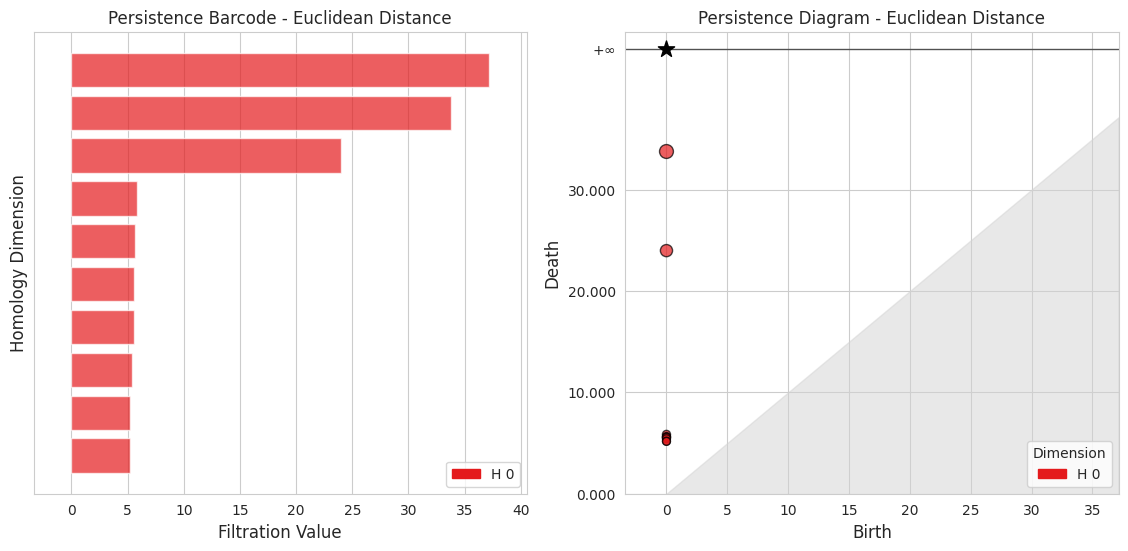
\includegraphics[width=0.9\linewidth]{figures/sample_1.png}
%     %     \caption{Persistence Barcode \& Persistence Diagram from ViT (Vision Transformer)}
%     %     \label{fig:enter-label}
%     % \end{figure}

            
%     \end{block}

% \end{column}




%   % \begin{block}{Machine Learning Interpretability}

%   %   In machine learning, understanding how models make decisions is crucial. Interpretability reveals the reasoning behind predictions, while explainability provides insights into model behavior.
    

%   %   \begin{figure}
%   %     \centering
%   %     \begin{tikzpicture}[scale=6]
%   %       \draw[step=0.25cm,color=gray] (-1,-1) grid (1,1);
%   %       \draw (1,0) -- (0.2,0.2) -- (0,1) -- (-0.2,0.2) -- (-1,0)
%   %         -- (-0.2,-0.2) -- (0,-1) -- (0.2,-0.2) -- cycle;
%   %     \end{tikzpicture}
%   %     \caption{A figure caption.}
%   %   \end{figure}

%   %   Lorem ipsum dolor sit amet, consectetur adipiscing elit. Morbi ultricies
%   %   eget libero ac ullamcorper. Integer et euismod ante. Aenean vestibulum
%   %   lobortis augue, ut lobortis turpis rhoncus sed. Proin feugiat nibh a
%   %   lacinia dignissim. Proin scelerisque, risus eget tempor fermentum, ex
%   %   turpis condimentum urna, quis malesuada sapien arcu eu purus.

%   % \end{block}

%   % \begin{block}{A block containing a list}

%   %   Nam vulputate nunc felis, non condimentum lacus porta ultrices. Nullam sed
%   %   sagittis metus. Etiam consectetur gravida urna quis suscipit.

%   %   \begin{itemize}
%   %     \item \textbf{Mauris tempor} risus nulla, sed ornare
%   %     \item \textbf{Libero tincidunt} a duis congue vitae
%   %     \item \textbf{Dui ac pretium} morbi justo neque, ullamcorper
%   %   \end{itemize}

%   %   Eget augue porta, bibendum venenatis tortor.

%   % \end{block}

%   % \begin{alertblock}{A highlighted block}

%   %   This block catches your eye, so \textbf{important stuff} should probably go
%   %   here.

%   %   Curabitur eu libero vehicula, cursus est fringilla, luctus est. Morbi
%   %   consectetur mauris quam, at finibus elit auctor ac. Aliquam erat volutpat.
%   %   Aenean at nisl ut ex ullamcorper eleifend et eu augue. Aenean quis velit
%   %   tristique odio convallis ultrices a ac odio.

%   %   \begin{itemize}
%   %     \item \textbf{Fusce dapibus tellus} vel tellus semper finibus. In
%   %       consequat, nibh sed mattis luctus, augue diam fermentum lectus.
%   %     \item \textbf{In euismod erat metus} non ex. Vestibulum luctus augue in
%   %       mi condimentum, at sollicitudin lorem viverra.
%   %     \item \textbf{Suspendisse vulputate} mauris vel placerat consectetur.
%   %       Mauris semper, purus ac hendrerit molestie, elit mi dignissim odio, in
%   %       suscipit felis sapien vel ex.
%   %   \end{itemize}

%   %   Aenean tincidunt risus eros, at gravida lorem sagittis vel. Vestibulum ante
%   %   ipsum primis in faucibus orci luctus et ultrices posuere cubilia Curae.

%   % \end{alertblock}

%   \separatorcolumn

%   \begin{column}{\colwidth}
  
  
%       % \begin{exampleblock}{Test}
%       %     Test
%       % \end{exampleblock}
  
%       \begin{block} {Where is the PH applied?}

%         The activations from a deep learning model for a given input are retrived using a hook function. Then the pairwise distances for the given inputs are calculated using various distance metrics. The distance metrics are then forwarded to the filtration function.       
        
%         The choice of distance metric directly affects the filtration process and influences which topological features are captured and their persistence. 
        
%         By analyzing the same activation data with multiple distance metrics, we can triangulate a more complete understanding of how information flows through the network and which structural patterns contribute to the model's decisions.  
 
        
%         \begin{figure}
%             \centering
%             % 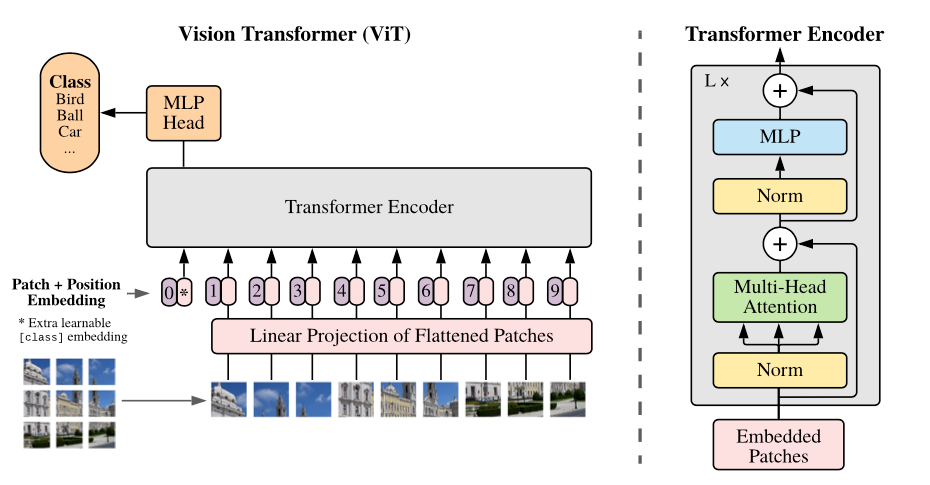
\includegraphics[width=0.5\linewidth]{figures/vit_architecture.png}
%             \includestandalone[mode=buildnew, width=\textwidth]{figures/arch}
%             \caption{Model Activations}
%             % \label{fig:enter-label}
%         \end{figure}

%         % \begin{figure}
%         %     \centering
%         %     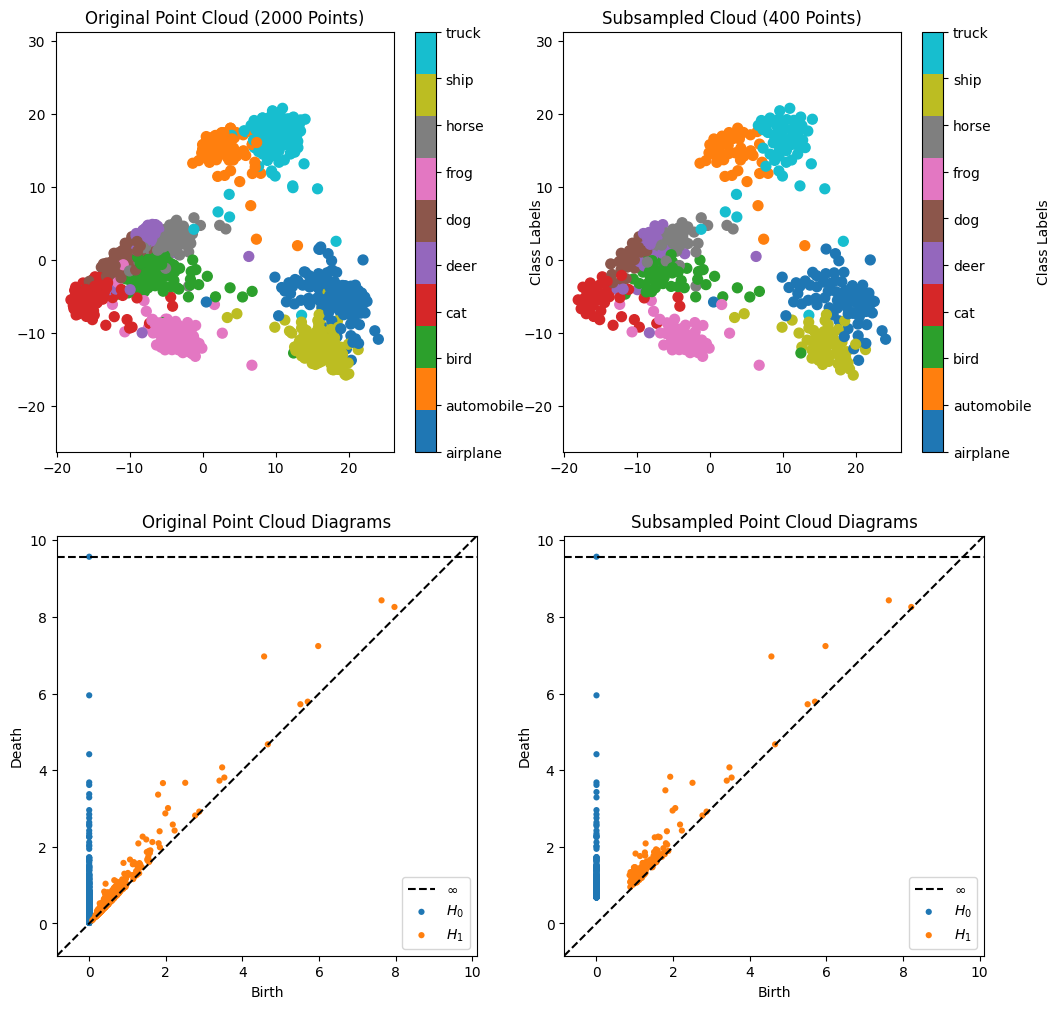
\includegraphics[width=0.5\linewidth]{figures/12_layer_vit.png}
%         %     \caption{ Persistent Homology on ViT model's Layer 12 activations.}
%         %     % \label{fig:enter-label}
%         % \end{figure}
       
%         \end{block}
    
%       \begin{figure}[h!]
%           \centering
%         %   \begin{minipage}{.45\linewidth}
%         %       \centering
%         %       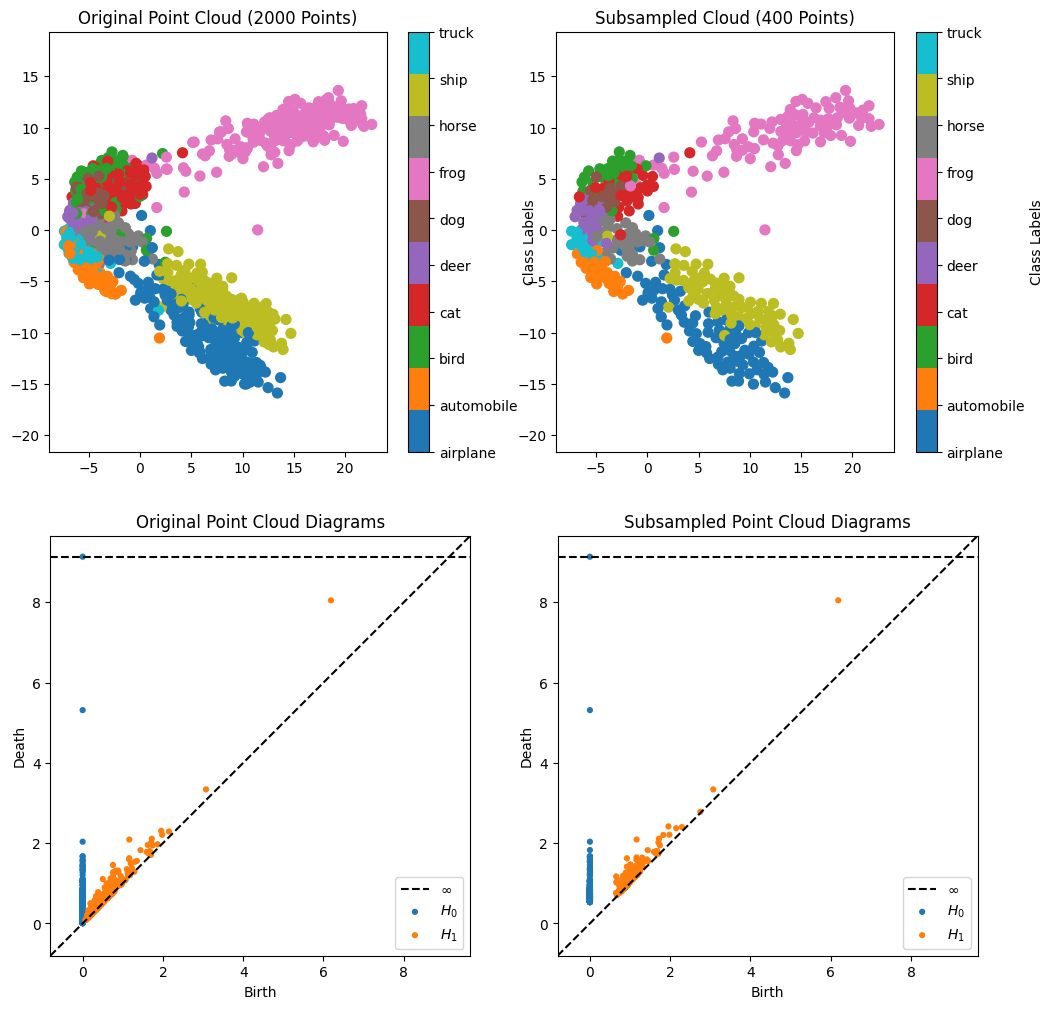
\includegraphics[width=\linewidth]{figures/11_layer_vit.png}
%         %       \caption{ViT layer 11}
%         %   \end{minipage}
%         \begin{minipage}{.45\linewidth}
%             \centering
%             \includegraphics[width=\linewidth]{figures/euclid_resnet.png}
%             \caption{Resnet50 (Trained on CIFAR10)}
%         \end{minipage}
%           \begin{minipage}{.45\linewidth}
%               \centering
%             %   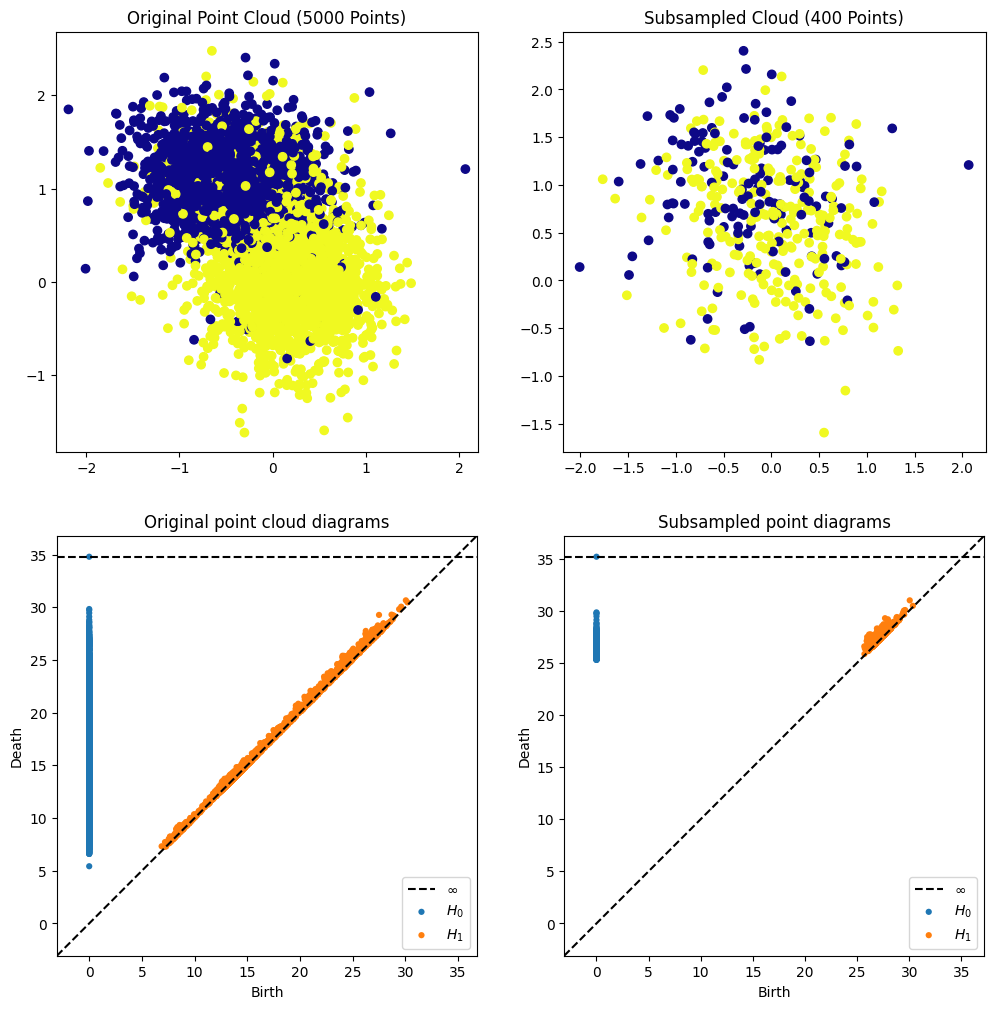
\includegraphics[width=\linewidth]{figures/genomic_model_nt.png}
%             %   \caption{Nucleotide Transformer (Genomic Model)}
%             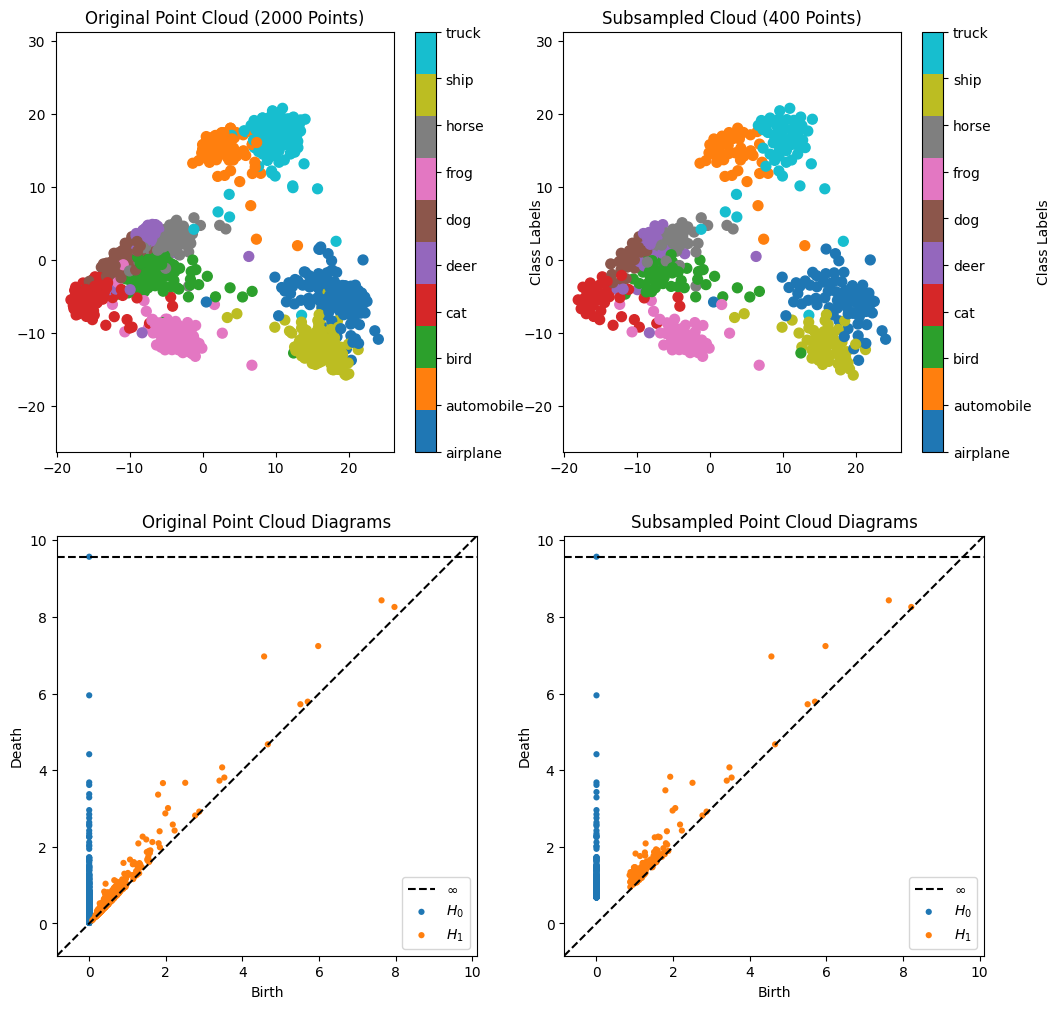
\includegraphics[width=\linewidth]{figures/12_layer_vit.png}
%             \caption{ Persistent Homology on ViT model's Layer 12 activations.}
%           \end{minipage}


%       \end{figure}
  


  
  
%       % \begin{figure}
%       %     \centering
%       %     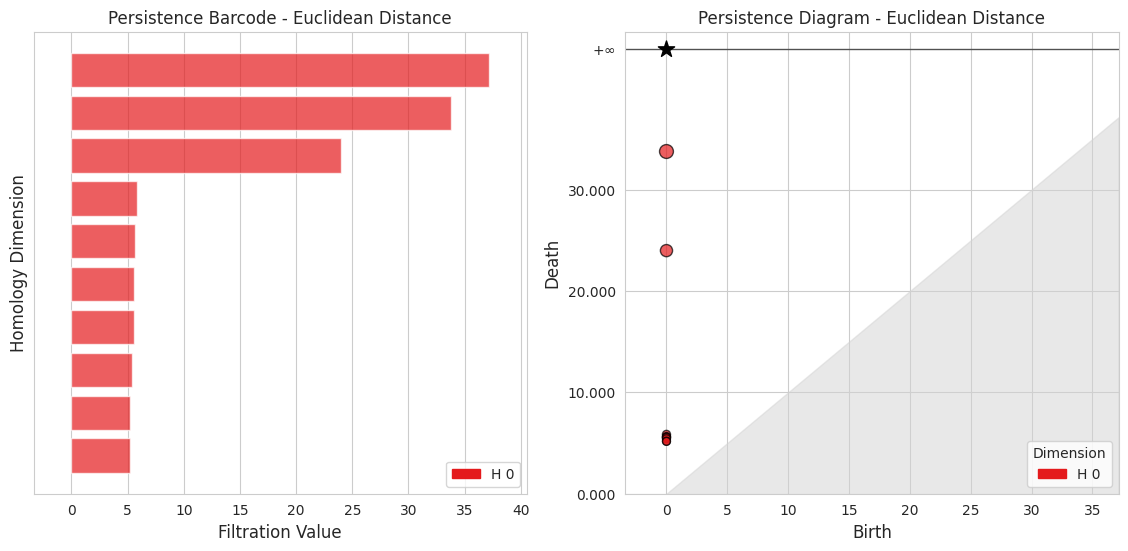
\includegraphics[width=0.3\linewidth]{figures/sample_1.png}
%       %     \caption{Enter Caption}
%       %     % \label{fig:enter-label}
%       % \end{figure}
  

  
  
  
  
%       % \begin{block} {Visualization Dashboard}
  
%       %     The clusters formed during the filtration process are visualized using sankey charts. Each stage in the sankey chart represents the $\mathcal{k}$-th death threshold.
  
  
%       %     \begin{figure}
%       %         \centering
%       %         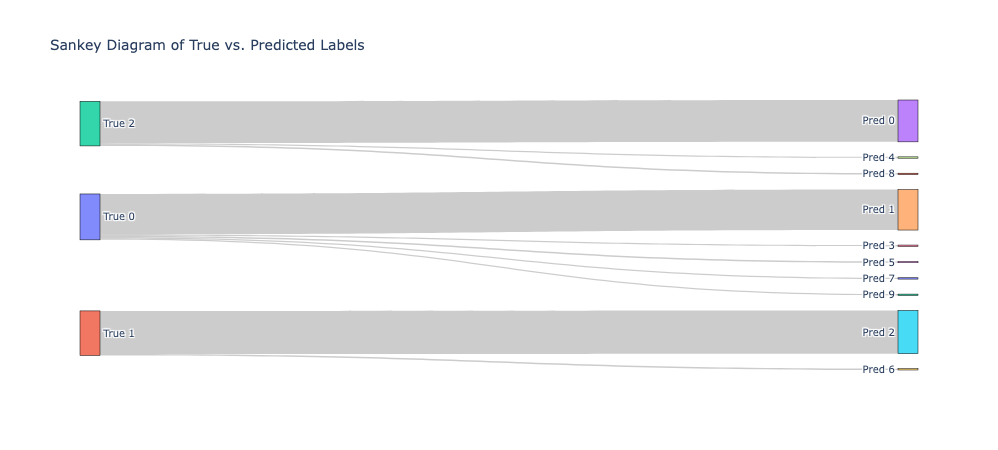
\includegraphics[width=0.5\linewidth]{figures/sankey.png}
%       %         \caption{Sankey Visualization}
%       %         % \label{fig:enter-label}
%       %     \end{figure}
  
%       % \end{block}
  
          
  
  
  
%     % \begin{exampleblock}{A highlighted block containing some math}
  
%     %   A different kind of highlighted block.
  
%     %   $$
%     %   \int_{-\infty}^{\infty} e^{-x^2}\,dx = \sqrt{\pi}
%     %   $$
  
%     %   Interdum et malesuada fames $\{1, 4, 9, \ldots\}$ ac ante ipsum primis in
%     %   faucibus. Cras eleifend dolor eu nulla suscipit suscipit. Sed lobortis non
%     %   felis id vulputate.
  
%     %   \heading{A heading inside a block}
  
%     %   Praesent consectetur mi $x^2 + y^2$ metus, nec vestibulum justo viverra
%     %   nec. Proin eget nulla pretium, egestas magna aliquam, mollis neque. Vivamus
%     %   dictum $\mathbf{u}^\intercal\mathbf{v}$ sagittis odio, vel porta erat
%     %   congue sed. Maecenas ut dolor quis arcu auctor porttitor.
  
%     %   \heading{Another heading inside a block}
  
%     %   Sed augue erat, scelerisque a purus ultricies, placerat porttitor neque.
%     %   Donec $P(y \mid x)$ fermentum consectetur $\nabla_x P(y \mid x)$ sapien
%     %   sagittis egestas. Duis eget leo euismod nunc viverra imperdiet nec id
%     %   justo.
  
%     % \end{exampleblock}
  
%     % \begin{block}{Nullam vel erat at velit convallis laoreet}
  
%     %   Class aptent taciti sociosqu ad litora torquent per conubia nostra, per
%     %   inceptos himenaeos. Phasellus libero enim, gravida sed erat sit amet,
%     %   scelerisque congue diam. Fusce dapibus dui ut augue pulvinar iaculis.
  
%     %   \begin{table}
%     %     \centering
%     %     \begin{tabular}{l r r c}
%     %       \toprule
%     %       \textbf{First column} & \textbf{Second column} & \textbf{Third column} & \textbf{Fourth} \\
%     %       \midrule
%     %       Foo & 13.37 & 384,394 & $\alpha$ \\
%     %       Bar & 2.17 & 1,392 & $\beta$ \\
%     %       Baz & 3.14 & 83,742 & $\delta$ \\
%     %       Qux & 7.59 & 974 & $\gamma$ \\
%     %       \bottomrule
%     %     \end{tabular}
%     %     \caption{A table caption.}
%     %   \end{table}
  
%     %   Donec quis posuere ligula. Nunc feugiat elit a mi malesuada consequat. Sed
%     %   imperdiet augue ac nibh aliquet tristique. Aenean eu tortor vulputate,
%     %   eleifend lorem in, dictum urna. Proin auctor ante in augue tincidunt
%     %   tempor. Proin pellentesque vulputate odio, ac gravida nulla posuere
%     %   efficitur. Aenean at velit vel dolor blandit molestie. Mauris laoreet
%     %   commodo quam, non luctus nibh ullamcorper in. Class aptent taciti sociosqu
%     %   ad litora torquent per conubia nostra, per inceptos himenaeos.
  
%     %   Nulla varius finibus volutpat. Mauris molestie lorem tincidunt, iaculis
%     %   libero at, gravida ante. Phasellus at felis eu neque suscipit suscipit.
%     %   Integer ullamcorper, dui nec pretium ornare, urna dolor consequat libero,
%     %   in feugiat elit lorem euismod lacus. Pellentesque sit amet dolor mollis,
%     %   auctor urna non, tempus sem.
  
%     % \end{block}
  
%     % \begin{block}{References}
  
%     %   \nocite{*}
%     %   \footnotesize{\bibliographystyle{plain}\bibliography{poster}}
  
%     % \end{block}
  
%   \end{column}

% \separatorcolumn
% \begin{column}{\colwidth}

%   \begin{block}{Distance Metrics in Filtration}
%     The choice of distance metric plays a crucial role in persistent homology by defining when simplices form connections in the filtration process. During our experiments we tried Euclidean distance, Mahalanobis distance, and a density-based normalization applied to the the former metrics.

%       \begin{enumerate}
%           \item \textbf{Euclidean Distance (\(L_2\) norm)}
%                 \[
%                 d_2(\mathbf{x}, \mathbf{y}) = \sqrt{\sum_{i} (x_i - y_i)^2}
%                 \]

%           \item \textbf{Mahalanobis Distance}
%                 \[
%                 d_M(\mathbf{x}, \mathbf{y}) = \sqrt{(\mathbf{x} - \mathbf{y})^T \mathbf{\Sigma}^{-1} (\mathbf{x} - \mathbf{y})}
%                 \]

%           \item \textbf{Cosine Distance}
%             \[
%             d_{\text{cos}}(\mathbf{x}, \mathbf{y}) = 1 - \frac{\mathbf{x} \cdot \mathbf{y}}{\|\mathbf{x}\| \|\mathbf{y}\|}
%             \]

%           \item \textbf{Relative Neighborhood-based distance normalization}: 

%             Here $\mathrm{k}$ is the $\mathrm{k}$-th nearest neighbour, a hyperparameter chosen by the user.
          
%             \[
%             d_{\text{VR-RNG}}(x, y) = \frac{d(x,y)}{\max \big( d(x, x_k), d(y, y_k) \big)}
%             \]

           
%        \end{enumerate}

%     %    \vspace{-50mm}
%        \begin{figure}[h!]
%            \centering
%            \includegraphics[width=0.7\linewidth]{figures/center_col.png}
%            \caption{Persistent Homology Sample}
%         %    \label{fig:ph_test}
%        \end{figure}
%   \end{block}


%   % \begin{block}{A block containing an enumerated list}

%   %   Vivamus congue volutpat elit non semper. Praesent molestie nec erat ac
%   %   interdum. In quis suscipit erat. \textbf{Phasellus mauris felis, molestie
%   %   ac pharetra quis}, tempus nec ante. Donec finibus ante vel purus mollis
%   %   fermentum. Sed felis mi, pharetra eget nibh a, feugiat eleifend dolor. Nam
%   %   mollis condimentum purus quis sodales. Nullam eu felis eu nulla eleifend
%   %   bibendum nec eu lorem. Vivamus felis velit, volutpat ut facilisis ac,
%   %   commodo in metus.

%   %   \begin{enumerate}
%   %     \item \textbf{Morbi mauris purus}, egestas at vehicula et, convallis
%   %       accumsan orci. Orci varius natoque penatibus et magnis dis parturient
%   %       montes, nascetur ridiculus mus.
%   %     \item \textbf{Cras vehicula blandit urna ut maximus}. Aliquam blandit nec
%   %       massa ac sollicitudin. Curabitur cursus, metus nec imperdiet bibendum,
%   %       velit lectus faucibus dolor, quis gravida metus mauris gravida turpis.
%   %     \item \textbf{Vestibulum et massa diam}. Phasellus fermentum augue non
%   %       nulla accumsan, non rhoncus lectus condimentum.
%   %   \end{enumerate}

%   % \end{block}

%   % \begin{block}{Fusce aliquam magna velit}

%   %   Et rutrum ex euismod vel. Pellentesque ultricies, velit in fermentum
%   %   vestibulum, lectus nisi pretium nibh, sit amet aliquam lectus augue vel
%   %   velit. Suspendisse rhoncus massa porttitor augue feugiat molestie. Sed
%   %   molestie ut orci nec malesuada. Sed ultricies feugiat est fringilla
%   %   posuere.

%   %   \begin{figure}
%   %     \centering
%   %     \begin{tikzpicture}
%   %       \begin{axis}[
%   %           scale only axis,
%   %           no markers,
%   %           domain=0:2*pi,
%   %           samples=100,
%   %           axis lines=center,
%   %           axis line style={-},
%   %           ticks=none]
%   %         \addplot[red] {sin(deg(x))};
%   %         \addplot[blue] {cos(deg(x))};
%   %       \end{axis}
%   %     \end{tikzpicture}
%   %     \caption{Another figure caption.}
%   %   \end{figure}

%   % \end{block}

%   % \begin{block}{Nam cursus consequat egestas}

%   %   Nulla eget sem quam. Ut aliquam volutpat nisi vestibulum convallis. Nunc a
%   %   lectus et eros facilisis hendrerit eu non urna. Interdum et malesuada fames
%   %   ac ante \textit{ipsum primis} in faucibus. Etiam sit amet velit eget sem
%   %   euismod tristique. Praesent enim erat, porta vel mattis sed, pharetra sed
%   %   ipsum. Morbi commodo condimentum massa, \textit{tempus venenatis} massa
%   %   hendrerit quis. Maecenas sed porta est. Praesent mollis interdum lectus,
%   %   sit amet sollicitudin risus tincidunt non.

%   %   Etiam sit amet tempus lorem, aliquet condimentum velit. Donec et nibh
%   %   consequat, sagittis ex eget, dictum orci. Etiam quis semper ante. Ut eu
%   %   mauris purus. Proin nec consectetur ligula. Mauris pretium molestie
%   %   ullamcorper. Integer nisi neque, aliquet et odio non, sagittis porta justo.

%   %   \begin{itemize}
%   %     \item \textbf{Sed consequat} id ante vel efficitur. Praesent congue massa
%   %       sed est scelerisque, elementum mollis augue iaculis.
%   %       \begin{itemize}
%   %         \item In sed est finibus, vulputate
%   %           nunc gravida, pulvinar lorem. In maximus nunc dolor, sed auctor eros
%   %           porttitor quis.
%   %         \item Fusce ornare dignissim nisi. Nam sit amet risus vel lacus
%   %           tempor tincidunt eu a arcu.
%   %         \item Donec rhoncus vestibulum erat, quis aliquam leo
%   %           gravida egestas.
%   %       \end{itemize}
%   %     \item \textbf{Sed luctus, elit sit amet} dictum maximus, diam dolor
%   %       faucibus purus, sed lobortis justo erat id turpis.
%   %     \item \textbf{Pellentesque facilisis dolor in leo} bibendum congue.
%   %       Maecenas congue finibus justo, vitae eleifend urna facilisis at.
%   %   \end{itemize}

%   % \end{block}

% \end{column}



% \separatorcolumn
% \end{columns}
% \end{frame}

% \end{document}
